%
%   地震成像理论及方法(PDF重制版)
%   作者:Jon F. Claerbout
%   项目主页:https://github.com/nicklinyi/IEI_zh
%   编译环境:TeX Live 2016
%   中文支持:xeLaTeX + ctex
%
%
% LaTeX配置文件
%
\documentclass[UTF8, a4paper, 11pt, twoside, punct = CCT]{ctexbook}
% 页面设置
\usepackage[top=3.0cm, bottom=2.0cm, left=3.5cm, right=2.5cm]{geometry}

\ctexset{
    contentsname = {目 \quad 录},
    listfigurename = {图目录},
    listtablename = {表目录},
    chapter/number = \arabic{chapter},
    section/format+ = \raggedright,
    subsection/beforeskip = 0.25ex,
    subsection/afterskip = 0.25ex,
    subsubsection/beforeskip = -.1ex,
    subsubsection/afterskip = .1ex,
}
\addtolength{\parskip}{3pt}             % 段落间距
%设置IEITitle为subsection格式
\newcommand{\IEITitle}[1]{\subsection*{#1}}
\newcommand{\IEICMD}[1]{\section{\texttt{#1}}}

% 文档相关信息
\newcommand{\IEIDOCTITLE}{\textbf{地震成像理论及方法}} % 文档标题
\newcommand{\IEIDOCAUTHOR}{Jon F. Claerbout}             % 文档作者
\newcommand{\IEIDOCVERSION}{1.0-dev}            % 文档版本
\newcommand{\IEIDOCDATE}{\today}                % 文档更新日期
\newcommand{\IEIVERSION}{101.6a}                % IEI版本

\usepackage{datetime2}      % \today格式为YYYY-MM-DD
\usepackage[dvipsnames, svgnames]{xcolor}  % 颜色

\usepackage{titletoc}           % 目录设置
\setcounter{tocdepth}{2}        % 目录深度
\titlecontents{chapter}[0em]    % 章
    {\vspace{0.2em}\bfseries\large}
    {\thecontentslabel\quad}
    {\hspace*{0em}}
    {\hfill \contentspage}
\titlecontents{section}[1em]    % 节
    {\normalsize}
    {\thecontentslabel\quad}
    {\hspace*{0em}}
    {\ \dotfill \ \contentspage}
    [\vspace{-0.3em}]
\titlecontents{subsection}[3em] % 小节
    {\small}
    {\thecontentslabel\quad}
    {\hspace*{0em}}
    {\ \dotfill \ \contentspage}
    [\vspace{-0.3em}]

% 双栏目录
\usepackage{multicol}
\makeatletter
\renewcommand{\tableofcontents}{%
\setlength{\columnsep}{2.5em}
\begin{multicols}{2}[\chapter*{\contentsname}]%
    \@starttoc{toc}%
\end{multicols}}
\makeatother

% 页眉页脚设置
\usepackage{titleps}
\newpagestyle{body}[\small]{
    \sethead
    [$\cdot$~\thepage~$\cdot$][][\S\,\thesection\quad\sectiontitle]
    {\CTEXthechapter\quad\chaptertitle}{}{$\cdot$~\thepage~$\cdot$}
    \setfoot{}{}{}\headrule
}

% 空白页
\makeatletter	% copy from lnotes
\def\cleardoublepage{
    \clearpage
    \if@twoside
        \ifodd
            \c@page
        \else
            \hbox{}
            \vspace*{\fill}
            \begin{center}
		    保护环境,从阅读电子文档开始!
            \end{center}
            \vspace{\fill}
            \thispagestyle{empty}
            \newpage
            \if@twocolumn
                \hbox{}
                \newpage
            \fi
        \fi
    \fi
}
\makeatother

% 超链接及书签
\usepackage[
    CJKbookmarks=true,
    colorlinks=true,
    linkcolor=blue,
    citecolor=blue,
    urlcolor=blue
]{hyperref}
\hypersetup{ % 文档元信息
    pdftitle={\IEIDOCTITLE v\IEIDOCVERSION},
    pdfauthor={\IEIDOCAUTHOR},
}

% 代码宏包
\usepackage{listings}
\lstset{
    basicstyle=\footnotesize\ttfamily,
    xleftmargin=2pc,                    % 整体布局
    xrightmargin=2pc,
    backgroundcolor=\color{Lavender},   % 背景色
    rulecolor=\color{Silver},           % 边框颜色
    frame=single,                       % 边框
    columns=flexible,
}
\lstdefinelanguage{IEI} {
    keywords={IEI>},   % IEI提示符
    otherkeywords={IEI>, IEI/SSS>},   % IEI提示符
    sensitive=true,
    comment=[l][{\color[rgb]{0,0.4,0}}]{//},
}
\lstnewenvironment{IEICode}{
    \lstset{
        language={IEI},                     % 语言
        keywordstyle=\color{blue},          % 关键字颜色
    }
}{}
\lstnewenvironment{IEISTX}{
    \lstset{delim=[is][\textcolor{gray}]{!}{!}}
}{}
\lstnewenvironment{IEIDFT}{}{}

\usepackage{minted}
\setminted{linenos, frame=leftline, xleftmargin=2pc, numbersep=6pt, breaklines=true}
\setminted[console]{linenos=false, frame=none, fontsize=\small}
\newenvironment{code}{\captionsetup{type=Listing}}{}

% 解决代码复制问题
% http://tex.stackexchange.com/questions/83204/
\usepackage{accsupp}
\newcommand\emptyaccsupp[1]{\BeginAccSupp{ActualText={}}#1\EndAccSupp{}}
\let\theHFancyVerbLine\theFancyVerbLine
\def\theFancyVerbLine{\rmfamily\tiny\emptyaccsupp{\arabic{FancyVerbLine}}}

\usepackage{enumitem}	% 列表宏包
% itemsep 设置列表间距; topsep 设置列表前间距
\setenumerate{
    itemsep=-3pt, partopsep=0pt, parsep=\parskip, topsep=0pt
}
\setitemize{
    itemsep=-3pt, partopsep=0pt, parsep=\parskip, topsep=0pt
}
\setdescription{
    itemsep=-3pt, partopsep=0pt, parsep=\parskip,
    topsep=0pt, itemindent=0pt
}

\usepackage{float}      % 图表浮动体

% 图片
\usepackage{graphicx}
\graphicspath{{figures/}}
\usepackage{tikz}
\usepackage{tikz-3dplot}

\usepackage{longtable}	% 长表格
\usepackage{tabularx}
\usepackage{booktabs}   % 三线表

% 图表标题
\usepackage[labelfont={small,bf}, textfont=small]{caption}
\captionsetup[figure]{aboveskip=6pt, belowskip=-12pt}
\captionsetup[table]{aboveskip=6pt, belowskip=-6pt}

% 数学相关
\usepackage{siunitx}    % 数字与单位
\sisetup{per-mode = symbol}

\usepackage{amsmath}

%重音
%\usepackage{accents}

% 符号
\usepackage{pifont}

\usepackage[perpage]{footmisc}	% 脚注在每一页单独编号
% 脚注中verb http://tex.stackexchange.com/questions/203
\usepackage{fancyvrb}
\VerbatimFootnotes

% 自定义quote环境
% http://tex.stackexchange.com/questions/16964/
\usepackage{framed}
\newcommand*\openquote{\makebox(25,-22){\scalebox{5}{``}}}
\newcommand*\closequote{\makebox(25,-22){\scalebox{5}{''}}}
\colorlet{shadecolor}{Azure}
\makeatletter
\newif\if@right
\def\shadequote{\@righttrue\shadequote@i}
\def\shadequote@i{\begin{snugshade}\begin{quote}\openquote}
    \def\endshadequote{%
\if@right\hfill\fi\closequote\end{quote}\end{snugshade}}
\@namedef{shadequote*}{\@rightfalse\shadequote@i}
\@namedef{endshadequote*}{\endshadequote}
\makeatother

% https://github.com/ElegantLaTeX/elegant/blob/master/elegantnote.cls
\usepackage{manfnt}
\newenvironment{note}{
    \par\ttfamily\itshape\noindent{
        \makebox[0pt][r]{
            \scriptsize\color{red!90}\textdbend\quad
        }\textbf{Note:}
    }
}{\par\vspace{.5\baselineskip}}

% 使用 !text! 代替 \texttt{text}
\lstMakeShortInline[basicstyle=\small\ttfamily]{!}

\begin{document}

\pdfbookmark[0]{封面}{cover}
\begin{titlepage}
\begin{center}
\vspace*{1.5cm}
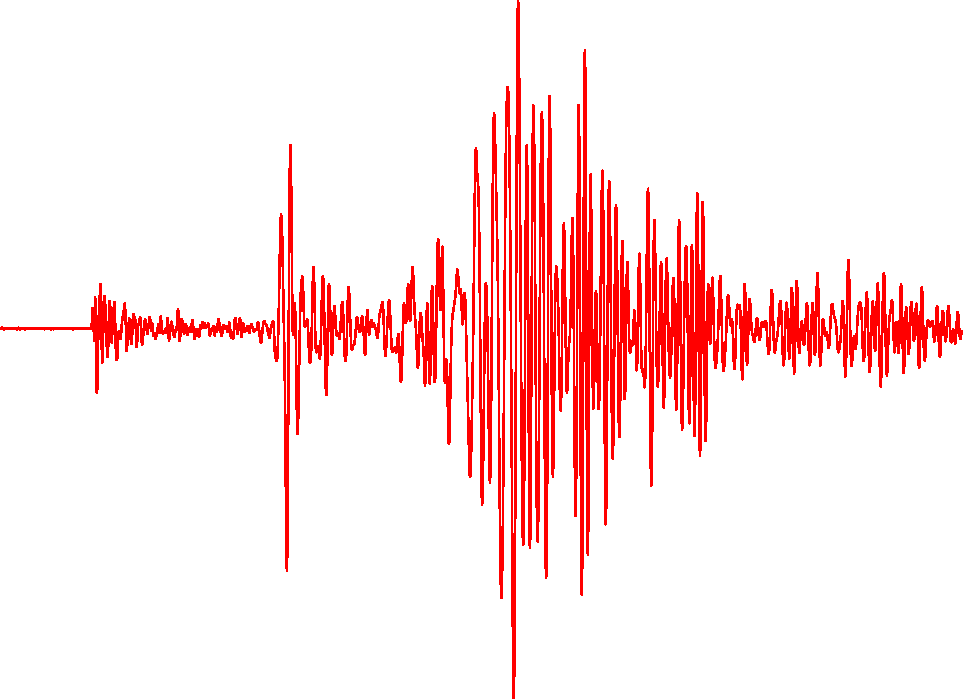
\includegraphics[width=0.8\textwidth]{IEI_logo}\\
\rule{8cm}{0.5mm}\\[0.35cm]
\Huge{\IEIDOCTITLE}\\
\rule{8cm}{0.5mm}\\
\Large{\hspace{2.5cm} 基于许云译著重制}\\[1cm]

\begin{minipage}{0.8\textwidth}
\begin{flushright}
\begin{tabular}{cl}
作者:& \IEIDOCAUTHOR \\
版本:& \IEIDOCVERSION \\
日期:& \IEIDOCDATE	\\
\end{tabular}
\end{flushright}
\end{minipage}
\end{center}
\end{titlepage}

\pagestyle{empty}

\frontmatter
{\ctexset{section/format+=\centering}\section*{序言}}

反射地震学家是要获得地层内部的映像。直到60年代为止,成像都是按一种特定方式
实现的。在1968年至1972年这段时期内,我构思出一种直接基于波动方程的新型成像方
法,并经过了野外观测的检验.以前都是从简化了的假想模型出发,利用波动方程来预测观
测结果,而在常规的数据分析中则未采用波动方程。我提出的有限差分的成像方法在石油勘
探工业中很快就得到了推广应用,随后,有许多其他人士也迅速参与其事,并作出了一些重
要改进。早期的特定成像方法经过重新解释,亦按照波动理论加以完善了。

由工业部门资助,在斯坦福大学成立了一个名为\textbf{SEP}
(斯坦福勘探计划)的小组,专门从事这项技术的研究。在48个资助单位中,许多单位都设有自己的具有良好素质的研究部
门。70年代中,取得许多进展的十年就这样开始了,在80年代,继续大步前进。

写作本书之目的萌生于向进入勘探领域的新手讲授这许多新概念中最精采部分的需要,
考虑到来自地球物理领域以外的人很多,我已使地球物理专门术语保持至最低限度,并且对
每个术语均作了定义。因此,料想本书不仅对有志于石油勘探的人们,而且对所有从事波场
分析之学科领域中的专业人士都将有所裨益

我以前写的《地球物理数据处理基础》\footnote{该书的中文译本于1979年由石油化学工业出版社出版.——译注}一书出版于1976年,最近业已重版。该书内容
涉及反射地震数处理的很多基本问题,诸如\textbf{Z}变换、傅氏变换、离散线性系统理论、矩
阵、统计学,以及厚状地层构造理论等等。该书也介绍过波动方程成像方法,然而,现在看
来,进行广泛增补已变得很有必要了,本书就是由这些增补演化而成。这两本书之间的不同
之处约占90咏,重复的部分占10\% 。这是出于使本书能独立成书之目的。

本书对石油勘探中所采用的数据处理技术的整个领域进行了紧凑精练的总结回顾,它是
斯坦福大学勘探地球物理课程中的基本教科书,不过,我并未奢求这本书是包罗万象的百科
全书,对于反褶积与静校正这样一些重要的处理方法,只是略加叙述,一带而过,对于层析
成象方法的实际应用这类内容亦复如是,而其他一些技术方法,诸如射线追踪(参阅\textbf{Cerveny},1977)及许多种类的正演模拟方法等,则均略而未提。很遗憾,仅有关偏移方法的文
献就已够浩瀚的了,以致对象\textbf{Kirchhoff}偏移方法在理论方面的一些显著贡献(参阅\textbf{Berkhout}, 1980 )也不得不舍弃了。

地震成像是一项从数学与物理学中汲取了许多内容的课题,这些题材按照一种逻辑顺序
将一项概念建立在另一项概念的基础之上;我是按类似顺序选择组织本书内容的,这样组
织内容有利于想透彻理解材料内容的新入学的学生。四处散布的一些有关实际问题难免为逻
辑结构所遗漏,为此,书末附有详细索引和上百篇涉及多种问题的参考文献,以供读者查
考。

更为广泛的论述反射地震学的专题教科书有\textbf{Waters} (1981
)与\textbf{Sengbush} ( 1983)的著
作。着重于石油勘探方面的描述性讨论反射地震学的书,有\textbf{Sheriff} (
1980 )与\textbf{Anstey} (1980 )等的著作。
\textbf{Aki}与\textbf{Richards} ( 1980)以及\textbf{Kermett} (1983)诸人写的书是关于天然地震学方面的补充读物.

我还试图使本书适合于那些想学习这些概念而对数学只想作略读的读者们的需要,个别
章节(各节都是一讲)在进行数学分析之前都尽可能地使之包含有实际问题的描述说明,各
章本身也是按此方式安排,因此,比方说,在你读第一章读到中途时,你可以跳过去直接去
读第二章。

波动现象恰好是美妙的几何学研究对象,利用很少一点数学分析就能学到很多内容,但
是,你应该是事前已经通晓了微积分、复指数和傅里叶变换等基本知识,之后再开始读本书
为好。

理论与实践之间总是存在有“空白”的。许多书都没给你提供有关“空白”之所在及其
范围的确切线索------即使是勘探地球物理方面的书籍也不例外。对这种“空白”,没必要感
到困惑不安,这正是研究课题活力所在------任何科学具有发展活力都是如此。“空白”就是
一个活动目标靶子,它涉及范围的大小就看你采取什么观点研究它了,所以,我得冒些风险
告诉你,该作什么,不该作什么;什么是重要的和什么是不重要的。观点总是超越于事实
的。你要是既不了解某些观点,又不了解实际,你的知识就不会是完整的知识。当我解释说
明理论与勘探实践之间的脱节时,以及当解释说明应该作什么而看来还没这样作的时候,你
将会既获得观点又获得事实\footnote{在中译本中做了节译。——译注}。





%{\ctexset{section/format+=\centering}\section*{版本说明}}

本文档目前在不断更新与完善中。

\begin{table}[H]
\centering
\begin{tabular}{cc}
\toprule
文档版本    &   文档发布日期    \\
\midrule
1.0         &   2016-06-28    \\

\bottomrule
\end{tabular}
\end{table}

{\ctexset{section/format+=\centering}\section*{维护者列表}}

本文档的源码开源托管在GitHub上,欢迎更多的用户参与到文档维护中,详情见
\href{https://github.com/nicklinyi/IEI_zh}。

\begin{table}[H]
\centering
\begin{tabular}{cccc}
\toprule
维护者      & 电子邮件              &   开始时间    &   结束时间     \\
\midrule
Nick  & \url{linyihanchuan@gmail.com}    &  2016-06-28   &   -     \\
\bottomrule
\end{tabular}
\end{table}


\pdfbookmark[0]{\contentsname}{contents}
\tableofcontents
\cleardoublepage
\pdfbookmark[0]{\listfigurename}{lof}
\listoffigures
\cleardoublepage
\pdfbookmark[0]{\listtablename}{lot}
\listoftables

\mainmatter
\pagestyle{body}


\chapter*{引论}
石油勘探是从地震测深开始的。用计算机将回声处理成可以揭示出许多地质历史的映
像。就全球范围而言,回声测深与映像处理就构成了大约每年40亿美元的经济活动。


\textbf{1.观测的意义}


石油与天然气的存在,对地震反射的直接影晌很小。岩石体积比烃类的体积要大很多
倍,不过,利用各种不同类型岩石之间的分界面,是可以很好对比追踪反射的。多孔隙岩石
中的烃类可以自由流动,流体有升起的趋向,岩石分界面的形状可以告诉我们什么地方可能
有烃类聚集。在北海中部发现石油与天然气是反射地震方法极为成功的一个例子。当以反射
地震学方法确定井位的第一口勘探井正在钻进之际,谁也不可能预料他们是否会钻遇石油,
可是,一旦当北海下面不论什么地方发现了石油,人们就会对如此确定的井位比随机定位的
那些井确实是更有利得多这一点抱有更大的信心。事实证明,的确如此。

在一口井已经钻完并完成了测井之后,反射映像就变得更为有价值了,因为根据它就可
以知道相应于每个回声反射应是什么岩石类型。地震学通常能够提供关于距井若干距离之处
岩石类型的出色的精确图像,特别有价值的是可以了解岩石沿什么方向上倾和地层在什么地
方被断层所断裂。地震学提供这种信息,其费用比多数钻井费用低得多。在转移至海上进行
石油勘探时,地震费用降低一个数量级,而钻井费用则要升高一个数量级。


\textbf{2.观测资料的可重复性}

反射地震资料数量庞大,它不是用铅笔在一张纸上画的记号,而是一盘接一盘的高密度
磁带。有些地震资料很容易理解,但是有许多却不那么容易,尤其是初次试验时的资料。虽
然许多资料不易理解而且看上去还有噪音和随机干扰,但值得注意的是这种资料在试验中是
可重复的。我们发现,用这种资料进行工作,可以认识到越来越多的东西,于是受到鼓舞而
继续做下去。因为在以常规方法采集的数据中仍然有许多信息隐藏其中,所以本书主要集中
于占主导地位的野外数据观布置,即通常具有近地表震源与接收器的单次测线。各种观测
技术仅作说明而不加以研究。


\textbf{3.作为成像工具的计算机}


哲学家提出问题:``何谓认识?''
。作为技术人员,我们的回答是:只要现实世界存
在,在我们心中也就存在它的一个映像。所谓认识,也就是意味着这二者是相似的。为有助
于形成映像,我们使用了显微镜、望远镜、辑影机、电视机等等这样一些成像装置。在本书
的描述中,计算机则是地震回声测深的成像工具。

计算机作为成像工具,在许多方面是颇为理想的。望远镜是受其组成部件质量限制的,
而计算机所形成的映像,很大程度上是受我们对数学、物理学和统计学的理解深度所限制,
而不是受计算机内在特性的限制。要是用雷达或者超声波来成像,计算机容量就会成为一个
现实问题,可是地震回声测深的信息含量(频带宽度)正好是大致与当今计算机的容量相匹
配。


\textbf{4.为何有趣?}


许多年轻人似乎都以揪住觫手的理论问题不放为乐事,可是一旦到了需要实际应用的时
候,他们往往失望地发现,这个理论在某些方面是离题的,或是不适合于当前的问题,一开
始的时候,这会减少对于实际问题的兴趣,但是最终许多人会达到这种境界:把实际问题看
成是比原有数学模型更为有兴趣的事。为什么会这样呢?

生活也许是像一种计算机游戏,我曾经注意到,学生们最喜爱的游戏并不是那些具有一
种预先决定的内在逻辑结构的游戏,他们喜欢可以允许他们在玩游戏时能逐步揭露其规律的
游戏。当由于应用自己个人的一些概念而使游戏老受挫折的时期能够告终,那确实是乐趣无
穷的。可是,要成为有趣的事,游戏就必须有若干规律,而你经过相当数量的努力必须能够
揭露出它们。很幸运,反射地震学连同现代计算机,就为我们提供了这样一个类似的环境。
有时,游戏可能总是失败,这时需要别人给你一点提示,使你克服某些障碍,进入一个新的
境界,达到较高的水平。阅读这本书并不像是玩这种游戏,它倒更像是给你题解大全或是锦
囊妙计,有助于你达到更高水平。

这些策略妙计大多数是新概念,其中许多概念的形成时间都不超出十年,所以选择它
们,是因为它们确实起作用,虽然并不总是、但往往是可令人满意的。我已经抑制了想把许
多虽尚未经充分试验但是颇有发展前途的策略妙计包括在内的强烈愿望了。

实践问题不但是比理论问题更深入一层,而且从根本上来说它们还会产生更为有意义的
理论。例如,我在大学一年级物理实验室内曾经想根据简单试验导出牛顿定律,我应从实验
中发现力等于质量乘加速度,当然,我没发现事实确实就是如此,试验似乎进行得并不顺
利,因为还存在有尚未考虑到的摩擦力。对你来说,现在摩擦确实就是一个有趣的主题了,
物理学家、化学家、冶金学家、地球科学家,全都了解牛顿定律,但愿他们都懂得摩擦
力!

你们现在所拥有的理论书籍,除两种较早期的理论处理方法如:成层介质数学物理理
论、时间序列分析之外,都还没有写出,也不可能涉及到我们数据资料中的一些最有趣的方
面。有的人认为我们仅仅有涂改玷污的数据!反射地震数据资料是可以重复回放的,我们的问
题中有许多实际是从理论产生的,而不是从数据产生的。


\textbf{5.计算机与电影}


这本书包括有一系列计算机程序,这些程序是用于解说例子和作为练习,也可作参考之
用。尽管还不能保证它们是尽善尽美,但是我作这本书中的许多图件时,它们曾起过作用,
因而它们应当也能为你服务。你将注意到,这是类似于FORTRAN的一种程序语言,在1.7
节开头部分就有这种程序的叙述说明。由于每人备有不同类型的图形输出装置,你自己要想
采用这种程序,那你就得精通这类装置,以便能将它们的输出接通至你的绘图设备。

电影实际就是许多画面的集合,在一台计算机中,它只不过就是一种必须以某种方式使
之转换为光亮画面(图形元素)的浮点数三维矩阵。目前,少数人已配备有可将这样一种三
维矩阵直接转换成电影的设备。在我的实验室中,这种转换是在一种高质量录像计算机终端
(AED512)上完成的。电影的潜在能力是一种很有价值的财富,它增强了我们对数据资料
的理解和对数据处理的理解。学生们因亲眼见到自己进行的程序工作能立即形成可用录像磁
带转录的一部电影,从而大大受到鼓舞。与其它图形显示装置相比,这种装置很容易维修
保养,进行研究工作的学生和攻读硕士学位课程的研究生都会使用它,利用它作课处作业练
习。

包括快速直接存取(DMA)计算机接口在内,这类设备的费用不超过一万美元。就真
正有效地采用这类显示方法的经验而言,你还应当具有可对内存大于几兆字节的一种计算机
进行物理控制的手段,如果你不是已经具备这点,处理成本费用将会增加大约十倍。


\textbf{6.有事可干吗?}


反射地震成像方法主要应用于石油勘探,烃类不同于核能,它是一种非再生能源,而且
还有迹象表明,在年轻一代有生之年期间,石油生产一定会下降。这是不是就意味着年轻人
应回避研究这方面的问题呢?我想,当然不是如此。就长期的观点来看,随着地球上人口的
继续增加,很难想像人们会失去对地壳进行研究的兴趣;就较为中期的观点看,随着能源蕴
藏丰富程度的减少,势必激起更大的勘探能涵的努力;就短期的观点看,从事能源勘探的工
作者在今天是很需要的,而且现在还不存在以煤或核能为能源的飞机。在任何情况下,本书
所讨论的技巧、物理概念在计算机上的实现方法等,将始终是具有普遍适用意义的。


\textbf{7.本书阅读指南}


第一章与第三章阐述反射地震学成像的基本概念。第二章与第四章的内容为分析被观测
波所需之计算机方法技术。第五章阐述先进的成像概念。在斯坦福大学,第一章至第三章悬
硕士研究生一个学期的讲授课程内容,在选修根据本书开课之前或之后,这些学
生同时还选修一门根据《地球物理数理基础》开出的课程。你也许想不学习有关方法技术
就能对概念有所理解,那你就不妨试着只读第一章和第三章容,不过,第二章内容因其具
体性质和它所包含的例子,将会增进你的理解能力,不妨也读一读。第四章内容适合于那些
想了解高质量完成任务时涉及到一些什么问题的技术人员,或者适合于那些希望通晓各种方
法的技巧与精度限制的非常熟练的解释人员。第五章阐述一些新颖的成像概念,它们在原理
上看来是正确的,但是因各种并非全都能为我所知的原因,它们均尚未获得广泛实际应用。
容忍得了数学的解释人员也许会赞赏第五章,因为这一章的宗旨就是解释事情是如何积为什
么总是按他们在实践中作的那种方式而完成的,不过,对于那些希望去发展新型回声成像方
法技术的人,第五章内容才真正会具有主要的吸引力。




\chapter{成像方法概论}
\section{爆炸反射面}
脉冲波震源、检波器(有时像个拾音器)和多记录道波形显示系统是反射地震勘探的基
本设备。测线沿地表布置,对海上勘探而言,测线可以是指勘探船航道,在这种情形下,接
收装置称作水听器。大约每25米震源激发一次,并在附近记录回声。由于穿透地层的池震波
波长比勘探船还长,震源和水听器几乎没有什么方向调谐能力,因此,回声可同时从几个方
向到达。解释这些观测结果,是地球物理学家和地质学家的共同任务。地球物理学家承担定
量的、物理的和统计方面的任务,他们的主要目标(因而也是主要指导写作本书的目标)就
是根据这些回声作出有关地层内部的良好图像。

\subsection{有力的类比}

图\ref{fig:xrf/expref}所示是两神波动传播情
形,第一种情况是实际的野外回声测深方法,第二种情况是一个想象的观
测记录情况------地层内的反射面突然
同时爆炸激发,从假设的爆炸震源产 生的波向上传播至地面,为假设的一
组检波器所接收。

\begin{figure}[H]
\centering
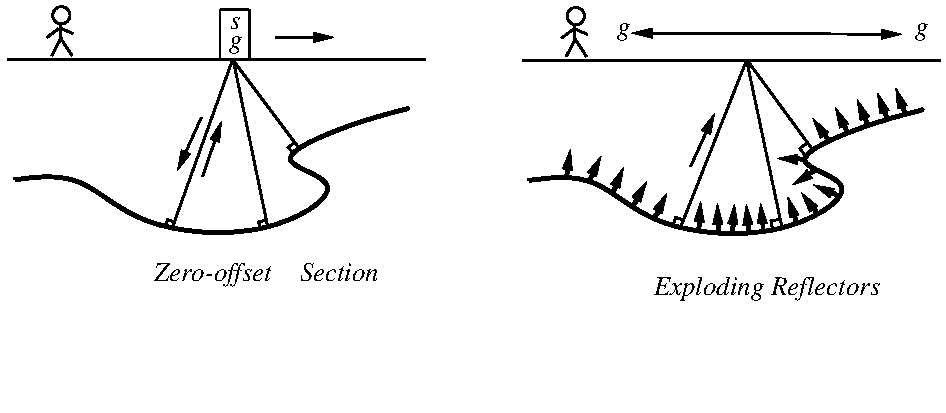
\includegraphics[width=0.95\textwidth]{xrf/expref}
\caption[爆炸反射面]{沿地表面所有位置移动的自激自收方式回声采集(左图),“爆炸反射面”想象模型(右图)}
\label{fig:xrf/expref}
\end{figure}
在图中要注意,实际野外记录情
形下的射线路程看起来同想象的爆炸 反射面情形下的那些射线路程是一样
的,把观测的与假设的这两种波场想像成确实是相同的波场,这在概念上有很大的好处。如果
它们相同,那么实际完成的成千炮记录就可忽略不计,从而可把注意力只集中于一个假设的记
录上。在实际的与想像的这两种情形 之间,有一种明显的差异,那就是:在实际野外观测系统中,
波必须首先 向下传播,然后沿同一路程向上返回
地表,而在假设的观测记录中,波只 向上传播;前者是双程射线路程,后
者是单程射线路程。野外实际观测记 录的旅朽时间应除以2;在实际工作
中,分析野外观测记录资料(双程时间)时都假设波速等于其真值的一半。

\subsection{惠更斯二次点源}
海面波浪具有可与地震勘探采用的波长相比的波长(15米至500米),不同之处就是海浪移动缓慢,容易观察。假设想
像有一很长的平行于海滩的码头防波堤,该堤有一很狭小的入口,恰可容许船只通过。这种
情形如图\ref{fig:xrf/storm}所示。来自开阔的公海而入射在防波堤上的。平面波将形成一个通过该堤空隙
的波。能观察到的一件事实就是:波阵面在码头内部变成为一个以该空隙为圆心的半圆弧。
波浪的这种波束与经过窗户射入的光线之间的差别只在于波长与孔穴大小之比值不同而已。

\begin{figure}[H]
\centering
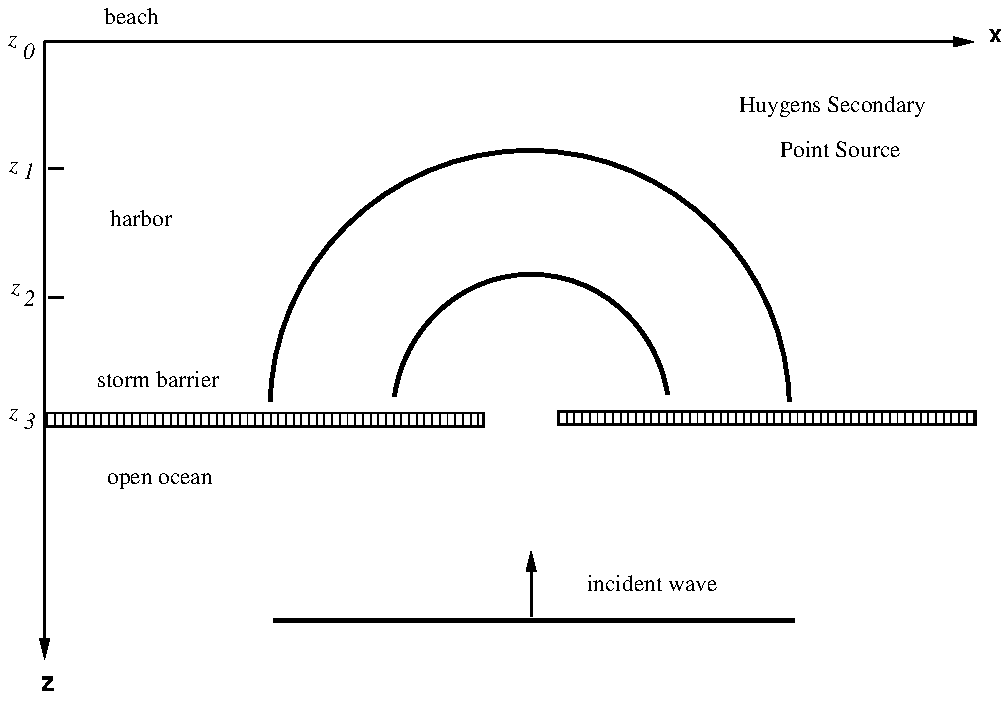
\includegraphics[width=0.6\textwidth]{xrf/storm}
\caption[惠更斯]{通过防波堤空隙的波具有半圆形波阵面(波长的长度可与空隙大小相比时)}
\label{fig:xrf/storm}
\end{figure}

线性性质是所有弱振幅波(不是指近岸处泡沫迸溅的碎浪)的一种性质,这意味着防波堤
有两个空隙就要形成两个半圆形波阵面,两圆相交处的波浪高度就等于两个高度的线性相加
结果。有趣的是考虑一下一个具有许多洞穴的防波堤,在洞穴非常多这种极限情形下,防波
堤消失了,剩下的只不过是一个紧挨着一个的空隙,许多半圆形波阵面形成的仅是入射平面
波。双曲线形的时距曲线亦复如此,图\ref{fig:xrf/storm2}所示是密度由左至右逐渐增大的许多双曲线,
所有非垂直角度方向上的波必然按某方式彼此叠加,使得除该平面波存在之外,其他一切均被压制抵消。

\begin{figure}[H]
\centering
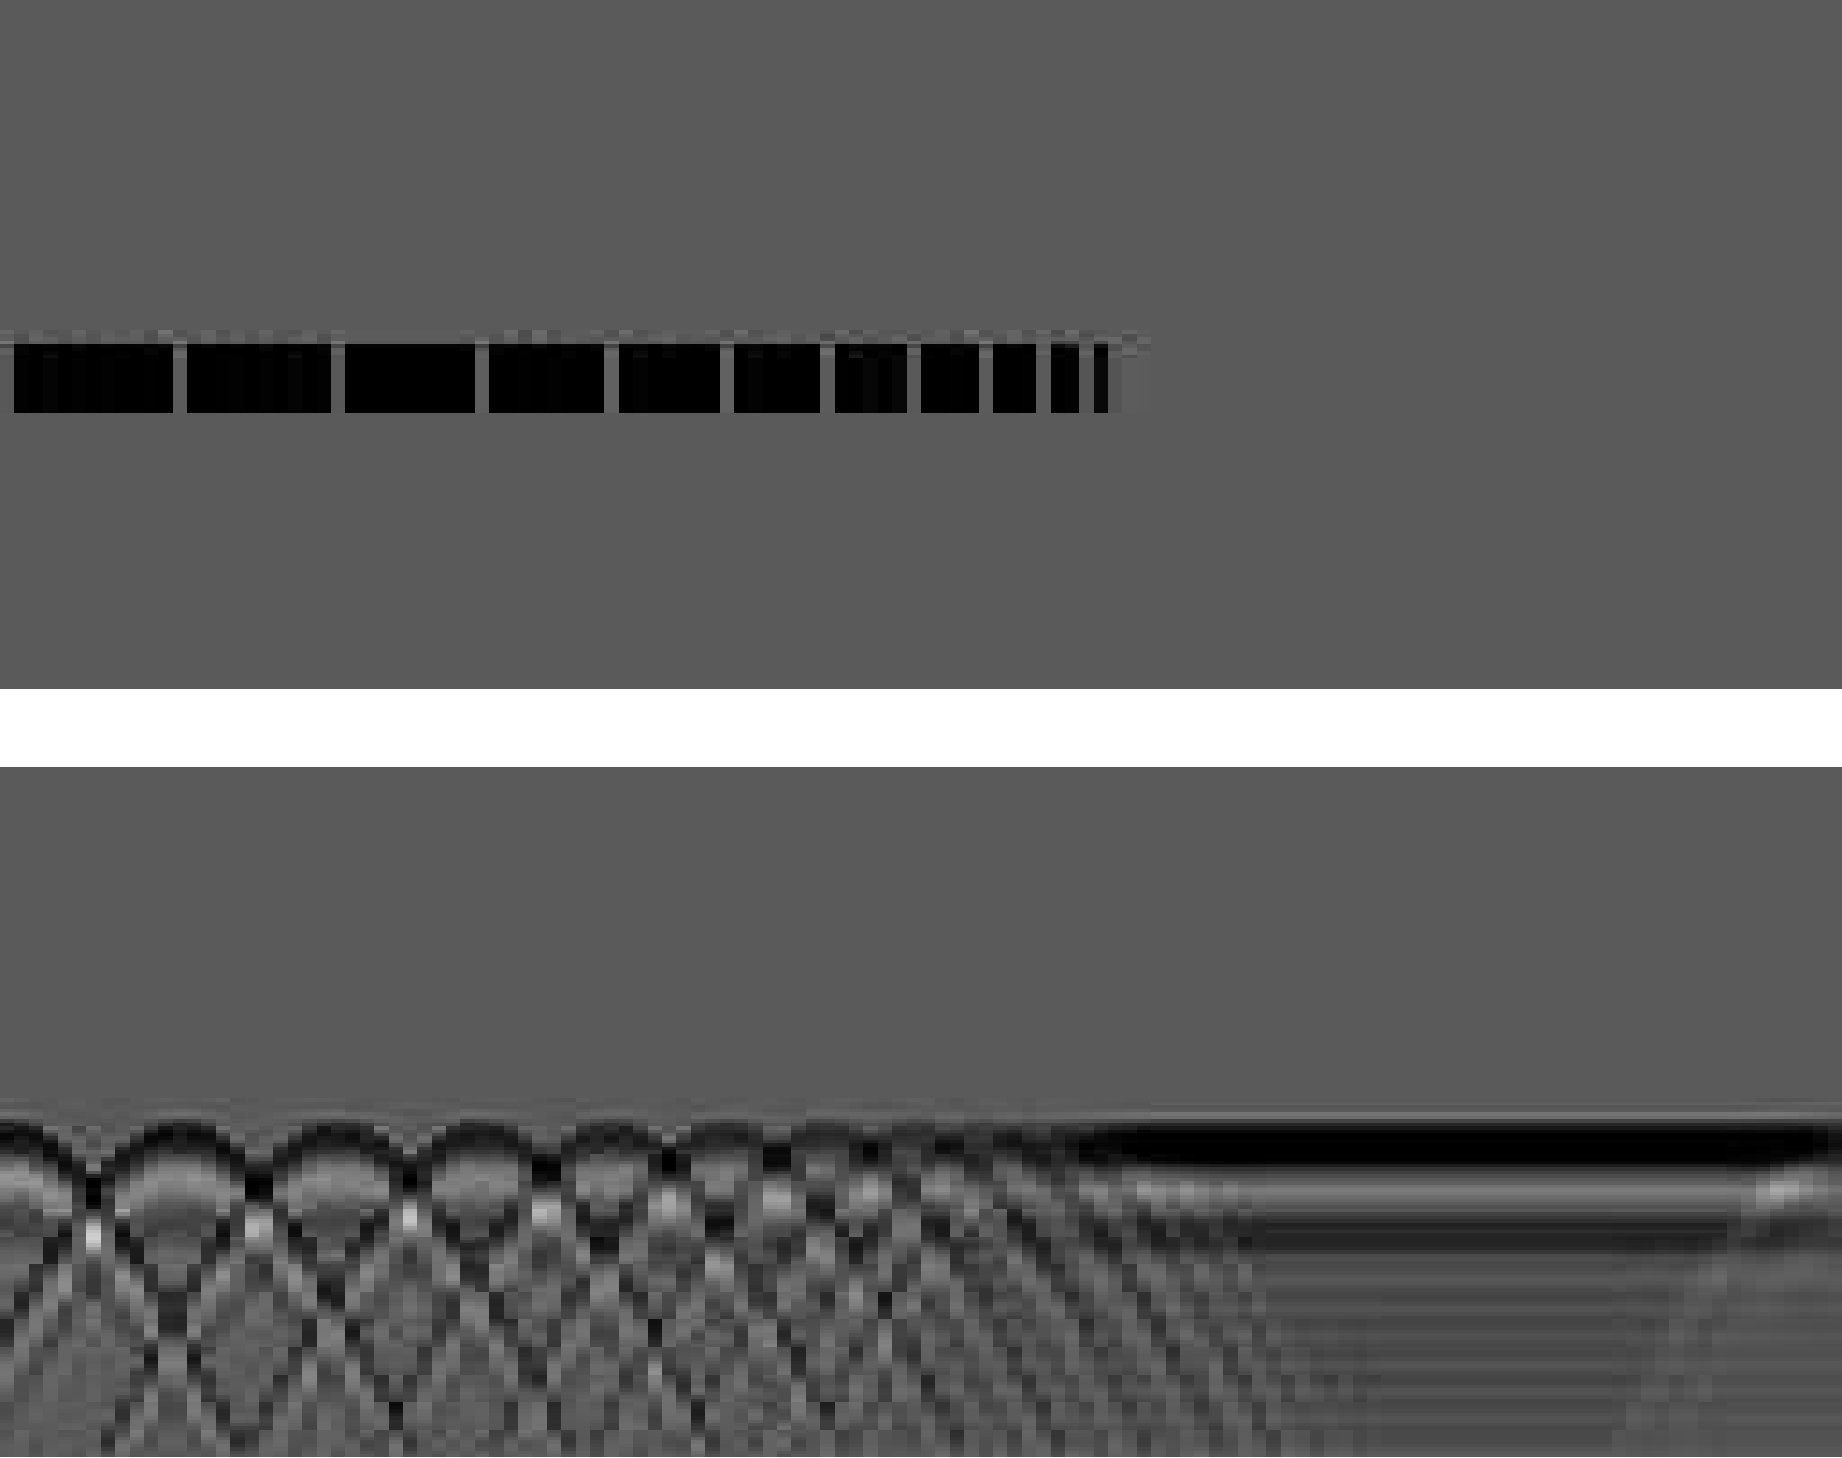
\includegraphics[width=0.95\textwidth]{xrf/storm2}
\caption[惠更斯]{具有许多洞穴的堤(顶部)及堤外所见到的$(x,t)$空间内的波(底部)}
\label{fig:xrf/storm2}
\end{figure}

设将直角坐标系统置于海面上,使海岸沿轴方向,而辅方向则可测度距海岸的距离。
为适合与反射地震学进行类比,假设人们活动只限于海岸(相当于反射地震中的地表面),
他们在那里进行波动观测------把波浪的高度作为坐标$x$与时间$t$的函数来加以观测记录。他们
根据这种数据可以作出关于在$(x,t)$平面内防波堤上存在有一个向外开口的空隙的推断。
图\ref{fig:xrf/dc}所示是波浪从海洋到达海岸的时间,最接近开口处之波浪最先到达,用什么数学
表达式来确定$(x,t)$平面内所见到約到达时间曲线形状呢?

\begin{figure}[H]
\centering
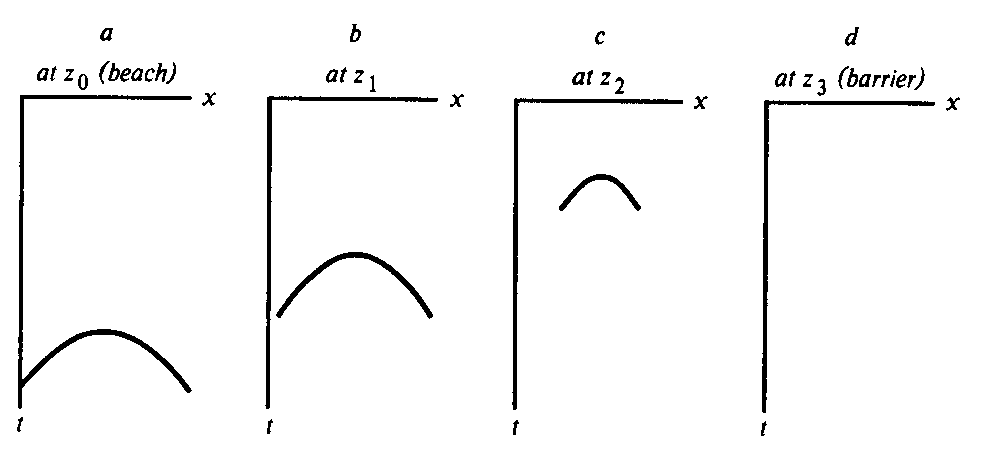
\includegraphics[width=0.95\textwidth]{xrf/dc}
\caption[dc]{左端的图表示在海岸上所见波浪之双曲线型时距曲线,右侧各图表示朝向海洋方向的距离子增大时,各个相继的到达时间曲线($x$轴业已压缩,不同于图\ref{fig:xrf/storm})(据Gonzalez)}
\label{fig:xrf/dc}
\end{figure}
波浪是一圈圈不断扩展着的圆。环绕点$(x_{3},z_{3})$以速度$v$不断扩张的圆其方程为:
\begin{equation}\label{eq:cir}
(x-x_{3})^{2}+(z-z_{3})^{2}=v^{2}t^{2}
\end{equation}
想像时间$t$为一常数时,即作一个快镜头拍摄时,则式\ref{eq:cir}就是那个圆的方程。设令$z$为
常数时,它就是在该$(x,t)$平面内的一个双曲线方程。若在三维体积内考
虑,式\ref{eq:cir}就是一个圆锥方程;各种不同$t$值时的横切面表现为各种不同大小的圆;各
种不同$z$值时的切片表示为各种不同的双曲线。图\ref{fig:xrf/dc}所示是四种双曲线,自左至右,第一
个双曲线是在海岸上$z_{0}=0$观测到的;第二个是在指向海洋方向的某个距离$z_{1}$上假想的一组
观测结果;第三个是在距海岸更远一些的距离$z_{2}$上假想的一组观测结果;第四个是在始终都
接近于防波堤的距离$z_{3}$上的一组观测结果,在该种情形下,双曲线业已蜕化为一个点。所有
这些双曲线均属于一个双曲线簇,每个双曲线均具有相同的渐近线。渐近线相应于在开口
空隙处转动将近90度角度的一种波,该波沿大约平行于海岸的方向移着,移动速度即波浪
速度$dx/dt$(为适合于对这种水波的类比,假定波浪的速度島一个与水深无关的常数)。

如果原始的入射波是个正脉冲,那么,惠更斯二次震源必然应由正极性与负极性二者组
成,才能使所有波动因相消干涉而彼此抵销,只有平面波存在。所以,惠更斯二次震源的波
形是有相移的。在下一节,将求出惠更斯二次震源的数学表达式。船工水手们熟悉的另一种
现象是:惠更斯半圆的最大振幅是位于直接指向海岸的方向上。由防波堤移动至海岸的波浪
系其振幅衰减至零,在光学中,这种随角度而出现的振幅减弱,称作倾斜因子(!obliquity!
 !factor!)。

\subsection{偏移定义}
!run!这个词,字典可以给出许多定义,它们彼此有关而又彼此有别。在地球物理勘探
中,!migration!(偏移)这个词同样也是大概有四种彼此有关而又彼此有区别的意思,最简
单的意思是像!move!(移动)这个词的意义。当位于$(x,z)$平面内某个位置上的物体在随后
时刻$t$时又位于另一个不同的位置上,于是我们就说它移动了。类似地,当位于地球物理观测
$(x,t)$空间内某个位置上的波至(往往也称作同相轴),又可在较大的深度$z$上出现在不同
位置上,于是我们就说它偏移了。

为更清楚看出这点,试想像图\ref{fig:xrf/dc}是取自一部影片的四个镜头画面。在影片放映时,
深度$z$就开始从海岸位置的深度(地表面)一直改变到防波堤位置的深度。把这些镜头画面叠合在一起,则
如图\ref{fig:xrf/dcretard}(a)所示。电影中发生的现象主要是同相轴朝$t=0$方向向上偏移了。
要消除这种占主导地位的垂直转移的影响,使各双曲线的顶点都保持在相同位置上进行另一种形式的叠加。
从数学上说,这就是用所谓的延迟时间轴$t^{'}=t+z/v$来代替时间轴$t$,如图\ref{fig:xrf/dcretard}(b)所示。

\begin{figure}[H]
\centering
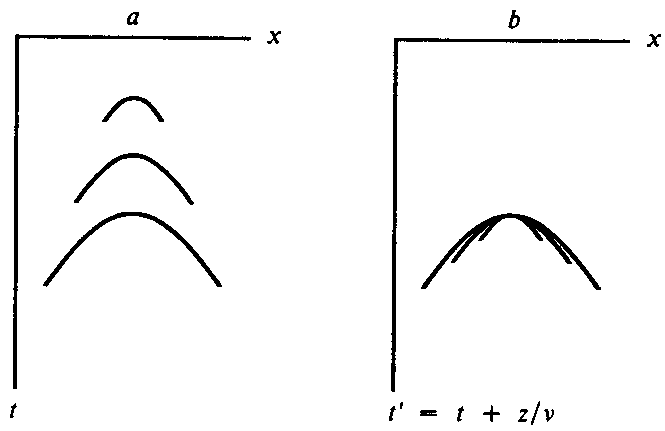
\includegraphics[width=0.95\textwidth]{xrf/dcretard}
\caption[dcretard]{(a)表示图\ref{fig:xrf/dc}中诸双曲线的叠合,(b)表示对叠合再配合以称作延迟$t^{'}=t+z/v$
的时移,使双曲线顶部彼此重叠(据Gonzalez)}
\label{fig:xrf/dcretard}
\end{figure}

第二种定义,也即更为准确的偏移定义是:在$(x,t^{'})$空间中的同相轴随深度$z$之改变而发生的移动。
在消除垂直时移之后,还有残余时间移动,那就主要是由某种波形变化引起的了。按照这种定义,双曲线
顶点或者水平地层是不偏移的。

图\ref{fig:xrf/dcretard}中的双曲线实际上是延伸至无限远的,但是图中每一个双曲线都在某个时间上
截断,这个时间等于$\sqrt{2}$乘该双曲线顶点的时间,所以图中所示双曲线仅是描述在与垂直方
向呈45度角的范围之内的射线。务必记住这一点:双曲线极小值时间与任何其它到达时间的比
值等于传播角度的余弦值。每个双曲线都是截止于45°出射角的射线。注意,图形上各双曲线
的端点可用一条直线连起来,还有,各双曲线端点上的斜率均相同,对于任何波阵面,波的传播角度在物理空间内为
$tan\theta =dx/dz$;对于任何地震同相轴,当你阵面以角度$\theta$与地面相交时,你就会发现,斜率$vdt/dx$
就等于$sin\theta$。所以,在物理空间$(x,z)$内沿一直线移动的能量就沿数据空间$(x,t)$内的一条直线而偏移。随$z$
之增大,沿所有角度传播的能量就一起聚集在一焦点上,这个焦点位于爆炸反射面,它就是防波堤内的开口空隙。这就是偏移
的第三种定义,即,偏移即是以某种方式将观测数据——作为$x$与$t$之函数的波浪高度——从海岸延展至防波堤的过程。第三种定义
并不过分强调移动本身,而是强调自起点至终点时的变换。

为更深入一步理解,只靠防波堤的例子是不行的,需要有更具普遍性的例子.防波堤的例子局限于仅在
某个特定深度$z$上形成惠更斯二次震源,但是为解释偏移的意义,还需要有在其他各种深度上的二次源。为此,现在提出一种可移动数据使$z$值不断增大的波场外推过程,按照下式构制爆炸反射面映像: 
\begin{equation}
Image(x,z)= Wave(t=0,x,z)
\label{eq:mig}
\end{equation}

这第四种偏移定义还与偏移的反义词,即绕射的定义有联系:

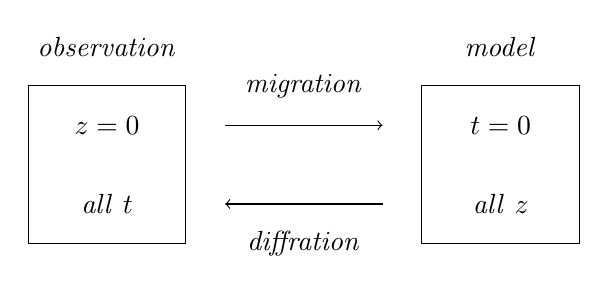
\begin{tikzpicture}
\centering
\draw (9,0) rectangle(11,2);
\draw (14,0) rectangle(16,2);
\draw[->] (11.5,1.5) -- (13.5,1.5);
\draw[<-] (11.5,0.5) -- (13.5,0.5);
\node at (10,0.5) {\emph{all} $t$};
\node at (10,1.5) {$z=0$};
\node at (15,0.5) {\emph{all} $z$};
\node at (15,1.5) {$t=0$};
\node at (10,2.5) {\emph{observation}};
\node at (15,2.5) {\emph{model}};
\node at (12.5,2) {\emph{migration}};
\node at (12.5,0) {\emph{diffration}};
\end{tikzpicture}

有时把绕射看作是形成与扩展双曲面的自然过程,偏移则是完成其反过程的计算机处理。


在第三章中将出现使用偏移一词的另一种情形,在该章中,水平坐标可以是炮点与检波点之间的中点$y$,
或者是炮检距$h$。在$(y,t)$平面和$(h,t)$平面内全都可以将双曲面向下
延拓,在$(y,t)$平面内,这种向下延拓称作偏移或成像,而在$(h,t)$平面内则将它称作聚焦或速度分析。


\subsection{数据资料中的脉冲}
惠更斯绕射在$(x,z)$空间内呈孤立的脉冲函数(即$\delta$函数)形式,从而$z=0$时在$(x,t)$
空间内就可使它成为一支双曲线。逆过程则需从$z=0$
时在$(x,t)$空间内的一个$\delta$函数开
始。这种倒过来的过程可以想像成是属于这样一类地震勘测:除了在一个特定位置上能记录
到回声之外,在任何其他位置上均记录不到,而在该特定位置上记录到的又仅只是一个回
声。同这样的观测结果符合一致的应该是什么样的地层模型呢?如图\ref{fig:xrf/semicirc}所示,这种地层
必须包含有一个球形反射面,球心就位于那个奇妙的记录位置上。
\begin{figure}[H]
\centering
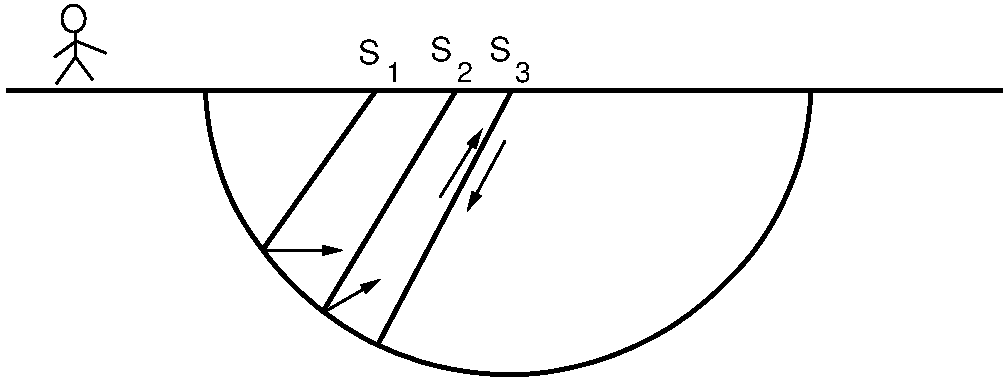
\includegraphics[width=0.6\textwidth]{xrf/semicirc}
\caption[semicirc]{当地震震源S准确位于半圆形反射面的圆心时,那时且仅仅在那时,才会有一个回声反射至
位于震源点上的检波器。这种半圆形反射面是根据仅只在地面一个位置上记录到一个回声这种数据记录方式作出的逻辑推论。}
\label{fig:xrf/semicirc}
\end{figure}

自然过程会在地层内部形成许多球形反射面,这看来是未必可能的。但是当我们注意业
经处理过的地球物理资料时,往往可看到剖面上有那么一些球形反射面。显然,这类输入数
据中包含有一些与此处所解释的波动传播理论不尽符合一致的脉冲。这点说明,为什么石油
勘探人员即使他们个人并不打算编写什么
处理程序,可他们却不得不研究反射地震数据处理方法。要理解认识原始数据资
料,那太复杂了。经过处理的资料可以给
出一个地层模型,但是它的可靠性难以断
定。你也许从未打算去造一辆汽车,但是
当你独自驾车远行进入沙漠时,那还是谨
慎一点好,应该尽你所能去了解熟悉关于
汽车的知识才是。

\subsection{手工偏移}

已知在点$(x_{0},t_{0})$上的地震同相轴 其斜率为$p=dt/dx$,试确定偏移后之位置$(x_{m},t_{m})$。
设想有一平面波阵面与地表面呈夹角$\theta$,在时间$dt$内传播距离为$dx$假设速
度为$v$,我们就得出以可观测量表示的波动传播角度

\begin{equation}
sin\theta=\frac{vdt}{dx}=pv
\label{eq:ex3}
\end{equation}

垂直旅行路程因
\begin{subequations}
\begin{equation}
t_{m}=t_{0}cos\theta=t_{0}\sqrt{1-p^{2}v^{2}}
\label{eq:ex4a}
\end{equation}

而小于有角度倾斜时的路程。由旅行时间$t_{0}$及速度水平分量$vsin\theta$得出偏移之后的横向位置为

\begin{equation}
x_{m}=x_{0}-t_{0}vsin\theta=x_{0}-t_{0}pv^{2}
\label{eq:ex4b}
\end{equation}
\end{subequations}

考虑到双曲线是向其顶点作偏移,就会明白为什么式\ref{eq:ex4b}中包含有一负号。式\ref{eq:ex4a}与
式\ref{eq:ex4b}是反射地震资料人工偏移的基本方程,它们告诉你偏移至何点,但是它们并未告
诉你斜率$p$会如何变化。

\subsection{反射面变陡}

设有一垂直分界面,这是倾斜地层的一种极限情形,它的反射,即双曲线的一支渐近线,却具有非垂直的陡实偏移将使倾斜地层的视陡度增大。
我采用视陡度一词,是因为
它是在$(x,t)$平面内所看到的已经变陡了的地层的斜率。偏移结果实际是沿$z$轴方向
分布的,但是为形成偏移时间剖面,总是使$z/v$重合在$t$轴上。当我们说一个双曲线偏移至其
顶点时,我们考虑的当然是偏移时间剖面。让我们将变陡过程作为一个角度函数来加以研究
一下。

设原点$(x_{0},t_{0})$邻近有一点$(x_{0^{+}},t_{0^{+}})=x_{0}+\Delta, t_{0}+p\Delta$,根据方程\ref{eq:ex4b},这个邻域偏移至

\begin{subequations}\label{eq:ex5}
\begin{equation}
t_{m^{+}}=(t_{0}+p\Delta)\sqrt{1-p^{2}v^{2}} \label{eq:ex5a}
\end{equation}
\begin{equation}
x_{m^{+}}=x_{0}+\Delta-(t_{0}+p\Delta)p^{2}v^{2} \label{eq:ex5b}
\end{equation}
\end{subequations}

现在我们可计算出偏移之后的同相轴因倾斜而形成的斜率$p_{m}$为

\begin{equation}
p_{m}
=\frac{dt_{m^{+}}}{dx_{m^{+}}}
=\frac{dt_{m^{+}}/d\Delta}{dx_{m^{+}}/d\Delta}
=\frac{p}{\sqrt{1-p^{2}v^{2}}}
=\frac{tan\theta}{v}
\label{eq:ex6}
\end{equation}

所以,像直角坐标空间内的斜率一样,偏移时间剖面上的斜率暗示着倾斜角度的正切,而未
偏移的时间剖面上的斜率则是该角度的正弦。

倾斜层在偏移时有斜率变化而双曲线的两翼在向下延拓时却未改变斜率,这事看起来
似乎有点自相矛盾,其实不然。一个原因是偏移等于向下延拓再加上成像(选择$t=0$时);
另一个原因则是一个双曲线是在一个深度上由一个震源所形成的一种特殊同相轴,而倾斜层
却是由不同深度的许多震源的叠加结果所形成。图\ref{fig:xrf/dip}即是表明形成一线状反射面
的许多点如何由绕射形成为一线形反射,以及形成一线形反射的许多点是如何偏移至一线状反射面的。

\begin{figure}[H]
\centering
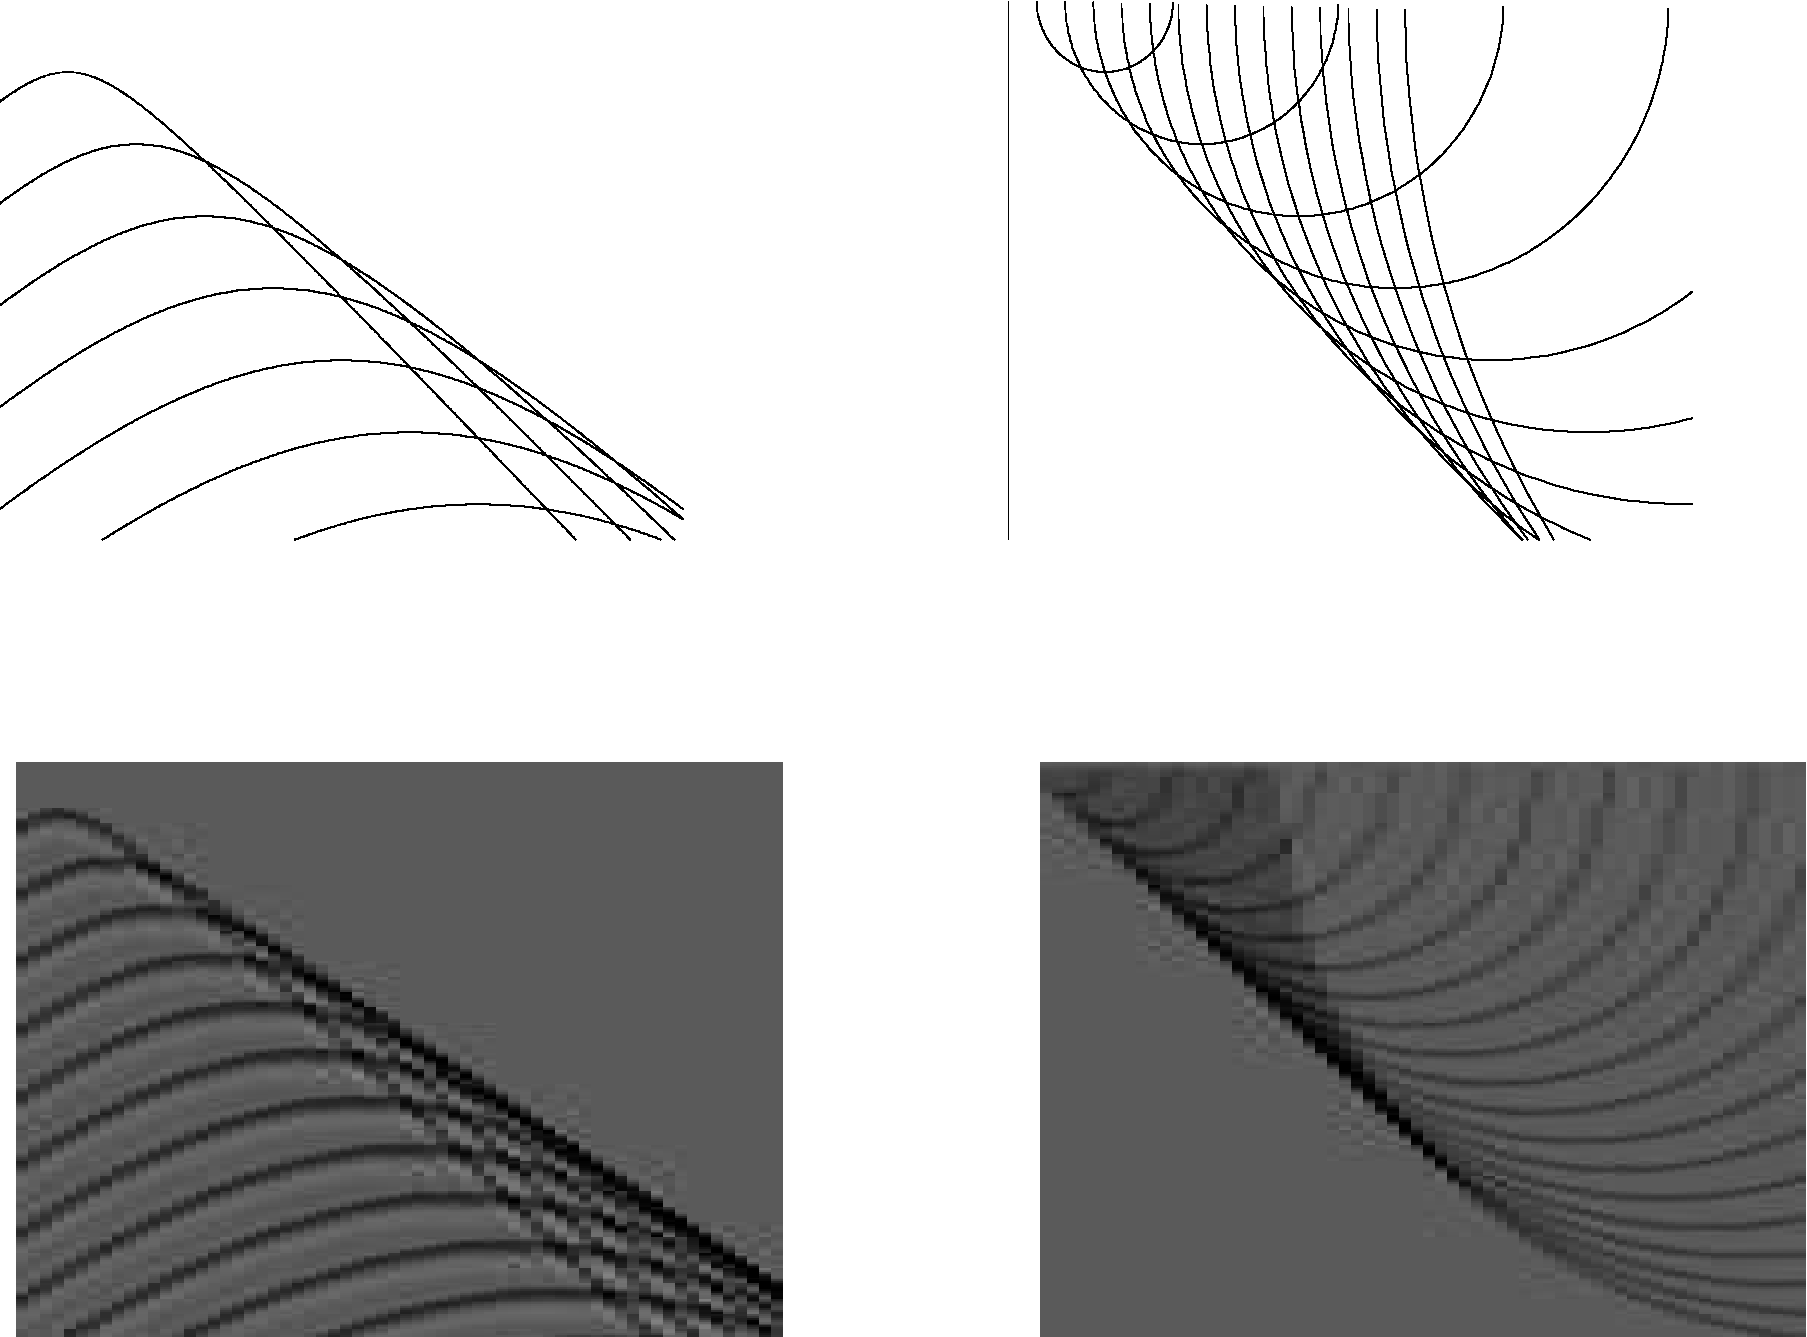
\includegraphics[width=0.95\textwidth]{xrf/dip}
\caption[dip]{
    左图是许多双曲线的叠加结果.各支双曲线顶部沿一条直线成布,该直线就像是反射面,不过并不是一条连
    续直线,而是一系列的点。相长干涉形成一个向一侧的视反射。
    右图表示许多半圆的叠加结果.各个半圆的底部沿一条直线分布,该直线代表观测到的平面波。不是平面波分
    解成一系列反射到达点,而是现在要把每个反射点解释成来自一个半圆状反射镜面。把所有反射镜面加起来,
    就形成了一个陡倾斜反射面。
}
\label{fig:xrf/dip}
\end{figure}
    
\subsection{爆炸反射面概念的限制}
    爆炸反射面概念是有力而又巧合的类比
    对于全部时间是从事于解释而不是从靡于处理
    的人来说,将爆炸反射面概念喻之为必不可少的拐棍还不够,它还是仅有的运输工具!可是
    对于我们这些从事于数据处理的人来说,这个爆炸反射面概念却有一个严重的缺点,现在还
    没有一个人已经解决了如何把这概念推广应用于非零炮检距记录资料的问题,
    资料却都是以相当大的炮检距进行记录的。在现代海上地震勘探中,不是用
    而是成百个串接在一条电缆上,拖在船后。记录系统的电缆长度典型的是二至三公里,勘探
    钻井可达三公里左右的深度,所以,实际上,地层倾角可以很大.这就涉及到新问题和新机
    会了,不过所有这些要到第三章才会讨论。
    
    再者,即使是零炮检距记录,这个爆炸反射面概念在定量上也不正确.该概念能有效成
    立的范围,将在第三章中阐述,此刻只对三个明显缺点作些注释:图\ref{fig:xrf/fail}所示是无法用爆
炸反射面模型加以预测的射线,这类射线在零炮检距剖面中却会出现。为适应这种情况,就
    只得假设存在有速度横向变化。

\begin{figure}[H]
\centering
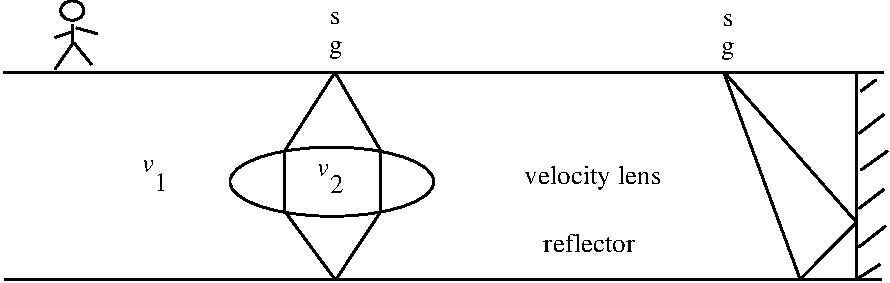
\includegraphics[width=0.95\textwidth]{xrf/fail}
\caption[fail]{
爆炸反射面模型解释不了的两支射线,然而零炮检距剖面上却可能存在这种射线。
}
\label{fig:xrf/fail}
\end{figure}
其次,爆炸反射面概念无法解释多次反射。设有双程波旅行时间为$t_{1}$的一个平缓海底,由
海底形成的多次反射应在时间$2t_{1},3t_{1},4t_{1}...$等可预测到,而按照该爆炸反射面概念
来解释,则第一次的多次反射应该从反射面至海面然后由海面至反射面,再从反射面至海面,总时间为
$3t_{1}$,从而相继的多次反射应在时间$5t_{1},7t_{1}...$
时出现。由此可知,零炮检距剖面上产生的多次反射不同于爆炸反射面模型产生的那些多次
反射。
    
我们能够看到波从分界面的两侧发生反射,这就涉及到爆炸反射面模型的第三个缺点,   
爆炸反射面模型预言由两侧出射的波具有相同极性,而根据反射系数的物理意义则只能说相
反两侧所形成的反射应具有相反极性。    
\subsection*{板块构造例子}
  板块构造理论认为,洋底是由海洋中部附近的脊火山上所形成的薄板块构成的,这些板
  块向海洋最深部的海糟移动,在那里它们倾没重返地壳。对该理论最有利的证据就是洋底缺
  失古老的岩石,一般而言,大陆都是被较年轻的移动海洋板块所推挤碰撞的古老岩石。有很
  多种方法可以极容易地观察到洋中脊火山作用形成的板块建造,至于板块是否真正在海槽中
  碰撞那就无法观测如此清晰了.证据均来自天然震源位置和反射地震学,图\ref{fig:xrf/japan}所示是
  日本海槽的一些反射资料,有两组反射占优势地位,即海底反射和向左方下倾的较深地层,
  后者可假设是开始倾没入地壳的一个板块的顶部;像近地面张力断裂那样,我们可将它作为
  向下挠曲的证据来加以研究(最顶部地层是与板块作松散接触的新近沉积海相软地层)。
  
\begin{figure}[H]
\centering
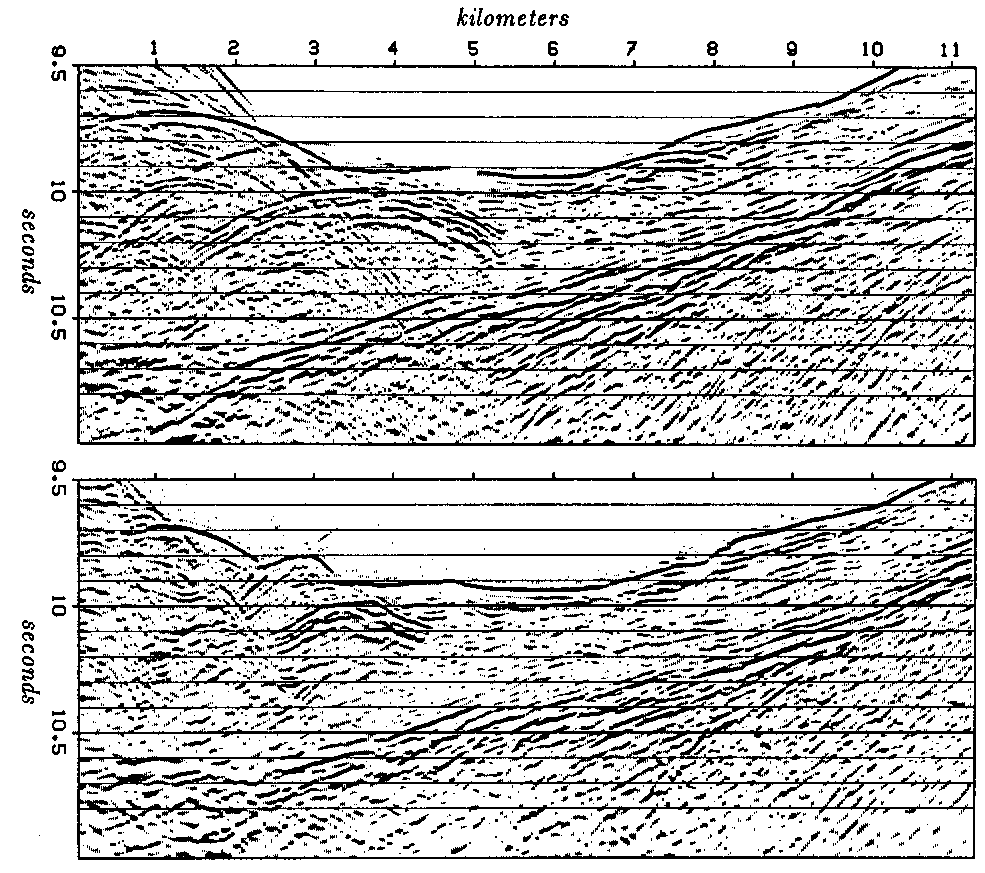
\includegraphics[width=0.95\textwidth]{xrf/japan}
\caption[japan]{
    上图是通过日本海槽的一条11公里长的测线的反射资料(东京大学海洋学研究所),下图所示为
    偏移处理之后的结果(Ottolini)
  }
\label{fig:xrf/japan}
\end{figure}
  注意,图\ref{fig:xrf/japan}的顶部不是零时间,时间轴是从9.5秒至11.0秒,在9.5秒以前没有反射
——我们要等待波在船与洋底之间传播。1公里至3公里周围的双曲线形反射同相轴因偏移归位形成为引人兴趣的``块状''。注意看一下8公里附近的海底地形和偏移与未偏移剖面之间的
  差异。偏移之后,的绕射双曲线就从4公里处的板块反射附近消失了,许多断裂(尤其
  是6.2公里处的一个断裂)都能更为明确地解释了。最后,如板块是向下挠曲,可是根据所
给资料,这点并不明显,要解决这个有关挠曲的疑问实际上还得要求对地震速度的横向变作更详尽的分析。

作为一个具体石油勘探意义的例子,看一下图\ref{fig:xrf/growth},这是德克萨斯州海上勘探的资
料,沉积物在沿岸河流进入墨西哥海湾处沉降,增加的重量引起沿着陡断层发生滑塌。在钻
井可以证实有一透水砂岩层之后,可将相应之反射沿上倾方向外推,与图\ref{fig:xrf/growth}资料上那
  样一些最邻近的断层倾斜相接.该断层很可能破坏了形成烃类向上运移聚集的渗透性通道的
  连续性。在这个深度上的砂岩可具有25热的孔隙率。假定地震波速度为2.2公里/秒,从而可
  导出图\ref{fig:xrf/growth}资料与实际物理体积之间的比例关系,对含油体积与图\ref{fig:xrf/growth}上同一体积的比
  值进行比较,可作出储量判断,由此你就可明白良好的成像是有多么重要了。

\begin{figure}[H]
\centering
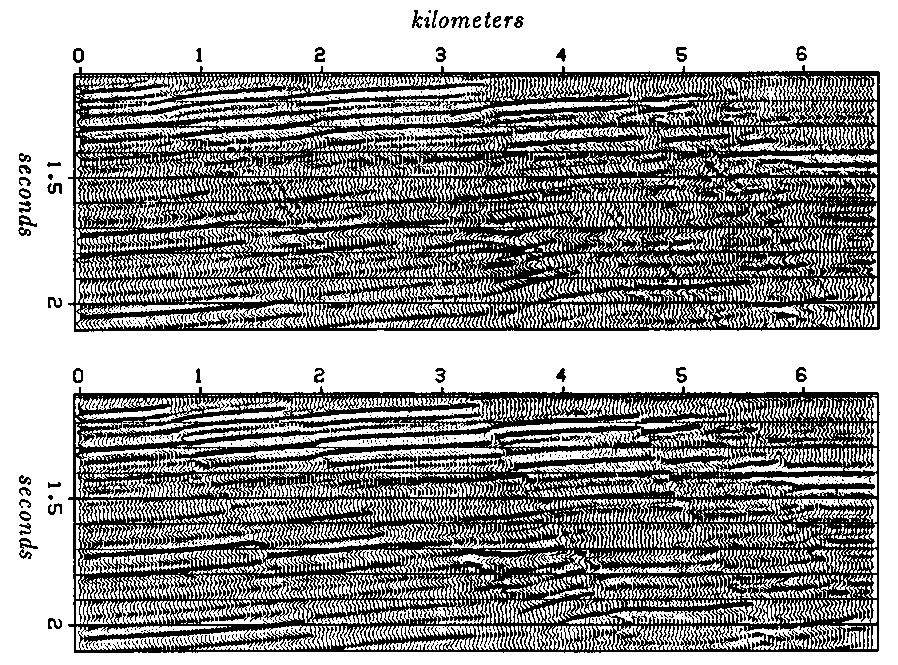
\includegraphics[width=0.95\textwidth]{xrf/growth}
\caption[growth]{
    上图是墨西哥海湾沿得克萨斯海岸海上勘探测线的6.5公里长的反射资料;下图为
      偏移处理的结果(Rothman )
  }
  \label{fig:xrf/growth}
\end{figure}

\subsection{习 题}

\begin{enumerate}
\item
    试证明毕达哥拉斯定理,即:直角三角形的斜边长度付决定于关系式$x^{2}+z^{2}=v^{2}t^{2}$。
\item 
    试计算图\ref{fig:xrf/japan}中双曲线两翼的传播角度
\item

利用习题2所得结果导出板块的倾伏角度。
\item 
试问日本海槽有多深(水层速度为1.5公里/秒)?
\item 
    试问在图\ref{fig:xrf/growth}上外海位于何方向?为什么?
\end{enumerate}

\begin{figure}[H]
\centering
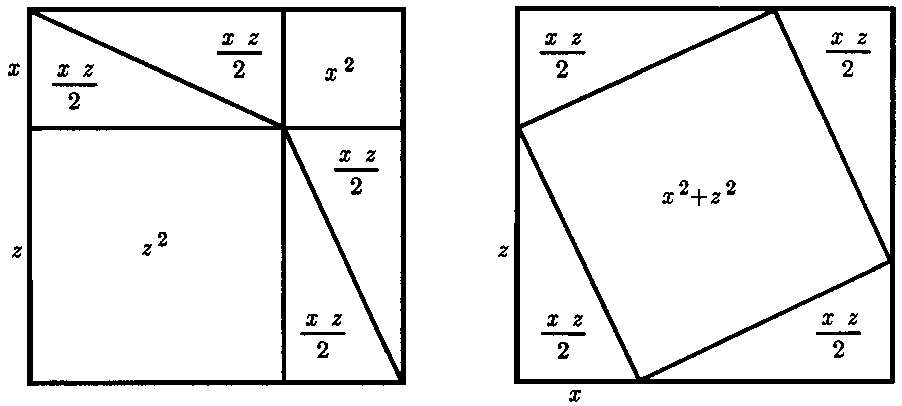
\includegraphics[width=0.95\textwidth]{xrf/pythag}
\caption*{
  
}
\label{fig:xrf/pythag}
\end{figure}


\section{起二维滤波作用的波场外推}
\label{sec:1.2}

一个脉冲函数($\delta$函数)可由许多正弦谐波(或复指数函数)的叠加构制出来,这是傅
氏分析的主要思想之一。在时间序列的研究中,就是用这种方法构制滤波器的脉冲响应。在
空间函数的研究中,则用这种方法来形成一个物理点源。

把时间特性与空间特性合在一起,就可将傅氏分量解释为单频平面波,物理光学(以及
与它有关的反射地震学)就成了滤波理论的一种推广情形。我们在本节中将研究惠更斯二次震
源在傅氏空间中的数学形式,就波场的空间外推而言,它就是一种二维滤波。

\subsection{射线与波前}
\label{sec:1.2.1}

\begin{figure}[H]
\centering
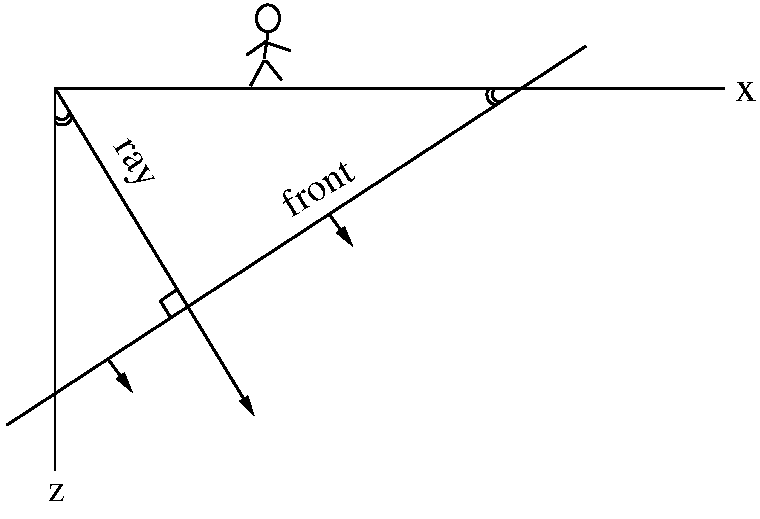
\includegraphics[width=0.5\textwidth]{omk/front}
\caption[front]{下行射线及其波阵面}
\label{fig:omk/front}
\end{figure}
  图\ref{fig:omk/front}所示是与垂直方向呈$\theta$角度向下移动进入地层的一个射线,垂直于该射线的是波
  阵面。根据基本的几何关系,波阵面与地表面之间的夹角也是。射线按速度$v$而增加其长度,在地表面上观察到的则是视速度,即波阵面与
  地面交点之移动速度,这种速度即为$v/sin\theta$,
  比速度$v$要快。类似地,波阵面与垂直轴之截
  点的速度(即垂直视速)为$v/cos\theta$。如图\ref{fig:omk/front}
  所示波阵面那样的直线,其数学表达式应为
  \begin{equation}
  z=z_{0}-xtan\theta
  \label{eq:ex1.2.1}
  \end{equation}
    在这表达式内,$z_{0}$是波阵面与垂直轴之间
    的截距.使该截点下行移动,用适当的速度乘以时间来代替它,则
  \begin{equation}
  z=v\frac{t}{cos\theta}-xtan\theta
  \label{eq:ex1.2.2}
  \end{equation}
    解出时间,得

  \begin{equation}
  t(x,z)=\frac{z}{v}cos\theta+\frac{x}{v}sin\theta
  \label{eq:ex1.2.3}
  \end{equation}

  式\ref{eq:ex1.2.3}可告诉我们关于波阵面通过任何特定位置$(x,z)$时的时间。对于任意形状具有时
  移的波形,其表达式以$f(t-t_{0})$表示。时移$t_{0}$用式\ref{eq:ex1.2.3}定义,可得出一个表示以某种
  波形沿射线移动的波场表达式

  \begin{equation}
  moving\ wavefield = f(t-\frac{z}{v}sin\theta-\frac{z}{v}cos\theta)
  \label{eq:ex1.2.4}
  \end{equation}

 \subsection{傅氏空间内的波}
 \label{sec:1.2.2}

 由正弦谐波的叠加,可构制出任意函数.经常出现的正弦谐波和复指数函数都是常系数
 线性偏微分方程的解,这就是它们出现的一个原因。之所以提到偏微分方程,是因为大多故
 物理定律都是可用偏微分方程表达的。


 对时间函数应用傅氏积另时,我们要遇到傅氏积分核$exp(-i\omega t)$。将式\ref{eq:ex1.2.4}中
 的任意函数具体化为函数$exp(-i\omega (t-t_{0}))$的实部,得

  \begin{equation}
  moving\ cosine\ wavefield = cos[\omega(\frac{x}{v}sin\theta+\frac{z}{v}cos\theta-t)]
  \label{eq:ex1.2.5}
  \end{equation}

  要把傅氏积分应用到空间坐标轴$x$必须定义空间圆频率。由于我们妓理问题时最终将会遇
  到大量空间坐标轴(炮点是三个坐标轴,检波点是三个坐标轴,中心点与炮检距也是三个坐标
  轴),所以就采用这样的约定:对字母$k$加一个下标示,用以表示对何种坐标进行傅氏变换.
  因此,$k_{x}$就是沿$x$坐标轴的空间圆频率,而$exp(+ik_{x}x)$则为其傅氏积分核。对每个坐标轴
  和傅氏积分核而言,还有一个$i$取什么符号的问题,此处采用大多数物理书籍中所采用的符
  号约定,即与式\ref{eq:ex1.2.5}
  所取符号一致的约定.如此选择的理由将在以后的\ref{sec:1.6}节中讨论。
  采用这种约定,波就是沿空间坐标的正方向移动,因而$(x,z,t)$空间的傅氏积分核将取
  为
  \begin{equation}
  Fourier\ kernel =
                e^{ik_{x}x}e^{ik_{z}z}e^{-i\omega t} = exp[i(k_{x}x+k_{z}z-\omega t)]
  \label{eq:ex1.2.6}
  \end{equation}

  使式\ref{eq:ex1.2.5}
  等于式\ref{eq:ex1.2.6}
  的实部,可知角度与速度均与傅氏分量有关,应该牢记这些关系!

  \begin{equation}
  sin\theta=\frac{vk_{x}}{\omega},cos\theta=\frac{vk_{z}}{\omega}
  \label{eq:ex1.2.7}
  \end{equation}

  由此可导出具有同等重要性的关系,将上述角度定义代入熟悉的关系式$sin^{2}\theta+cos^{2}\theta=1$
  ,就得出以标量波动方程波散关系而知名的一项极重要关系

  \begin{equation}
  k^2_{x}+k^2_{z}=\frac{\omega^{2}}{v^{2}}
  \label{eq:ex1.2.8}
  \end{equation}

  我们以后将会遇到波散关系和标量波动方程.式\ref{eq:ex1.2.8}的重要性在于:它能使我们区
  出一个实际是波场的无序函数同一个任意函数之间的差别.对任何一种函数$p(t,x,z)$,进行傅氏变换
  使之变为$P(\omega,k_{x},k_{z})$,现在对$P$的
  任何非零值所相应的$(\omega,k_{x},k_{z})$体
  作一下考察.显然,当且仅当$P$的所有非零值具有可满足式\ref{eq:ex1.2.8}
  的坐标时,它才会是一种波场。更有甚者,在实际情形
  下,$z=0$依从关系则是未知的。于是,假定$P$是一个波场就可以求出关于$z$的依从关系,因而根据
  式\ref{eq:ex1.2.8}能就关于$z$的依从关系作出推断。

\subsection{偏移可改善水平分辨率}
\label{sec:1.2.3}

在原理上,偏移就是将一些双曲线转换成一些点。在实际上,双曲线并不蜕化成点,它
们是蜕化成一个焦点。焦点具有可测度的大小尺度。说偏移效果“良好”,是因为它增加
了空间分辨率,它把一个很大的双曲线压缩成一个细小的焦点。为定量描述偏移改善分
辨率的作用,必须定双曲线的尺度和焦点的尺度。图\ref{fig:omk/fwidth}所示是测定
双曲线尺度的各种不同方法。
\begin{figure}[H]
\centering
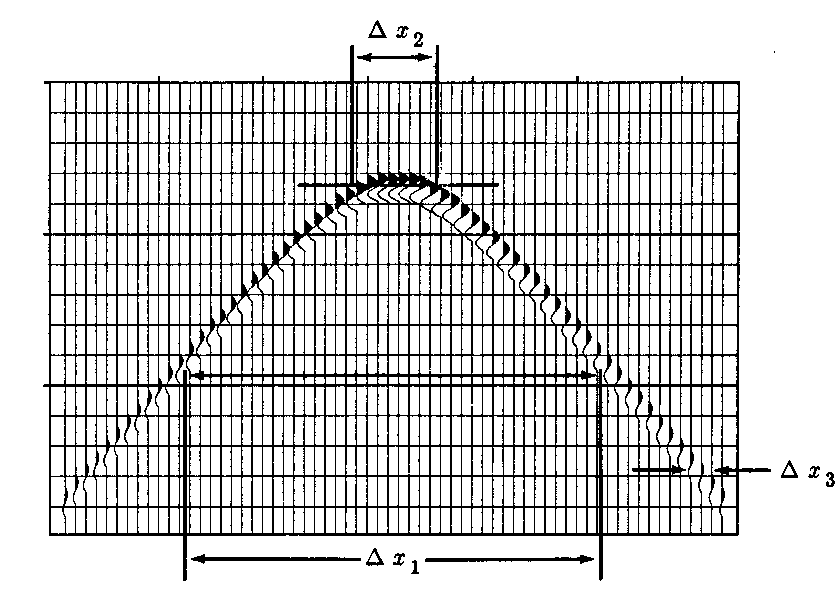
\includegraphics[width=0.6\textwidth]{omk/fwidth}
\caption[fwidth]{双曲线宽度参量的测定}
\label{fig:omk/fwidth}
\end{figure}
双曲线由地震脉冲组成,所以,根据主能量脉冲在时间轴上的各零交点之间的距离,可
租略大致估计双曲线的$\omega$频宽。典型的频宽值最50赫兹,不过你也可能遇到四倍
高一点或四倍低一点的值。决定深度分辨率的因素是关于地震波速度的知识,速度的典
型值为$3km/s$,不过你再一次可能会遇到四倍大一点或四倍小一点的速度。取这些值
意味着地震波长是实际波长的一半。之所以为一半,是由于在爆炸反射面计算中取了速度
$v$值的二分之一;或者与此等价,是由于将地震波长理解为被平分为上行部分与下行部分
了。习惯上,分辨率限定为有效波长的二分之一,或者大约为$15m$。地震分辨率是否应
取半波长$(15m)$或更小一些的值,这是个可以争论的问题,它涉及到关于信噪比的考虑,
超出了我们现在研究的范围。

横向分辨率需要估计双曲线宽度和焦点宽度。图\ref{fig:omk/fwidth}表示有三种双曲线
宽度定义,最宽的$\Delta x_{1}$大约包括双曲线四分之三的能量;其次是宽度$\Delta x_{2}$,
称作菲涅尔带(Fresnel Zone),它是初至正好改变极性时在两个时间上穿过双曲线的横截
距离。第三种是最小的可测宽度,位于远离双曲线顶部的侧翼上,这类宽度$\Delta x_{3}$
是所求出的最短水平方向波长。所谓分辨率就是误差范围大小的研究,所以,使误差本身
精确并没什么特别用处,主要知道$\Delta x_{1}>\Delta x_{2}>\Delta x_{3}$也就可以
了。空间波数$k_{x}$谱宽度大约为$1/\Delta x_{3}$。偏移究竟可以形成多么小的焦点呢
?这点将受到空间波数$k_{x}$谱中可达到的频宽所限制;焦点的范围大小将与$\Delta x_{3}$
大体相同。

图\ref{fig:omk/fresnel}是表示菲涅尔带概念的几何图形。菲涅尔带就是一个球面波与一
平面的相交截面、亦即球面波穿过该平面达到半波长深度时的截面。菲涅尔带宽度$\Delta x_{2}$
有什么意义呢?试想像你自己是在柏林市,那里有一堵“柏林墙”,你也许不被允许走近它。
假如墙上有一个洞,你现在向墙那一边的一位朋友大声打招呼。声音的响度是如何依赖于
墙洞的大小$\Delta X$呢?这并非明显易见,然而理论上和实验中众所周知的事实是:墙洞
比菲涅尔带大,就会引起声音稍微衰减,可是比较小的墙洞又会限制声音的传播,限制的
程度与该墙洞的大小成比例。
\begin{figure}[H]
\centering
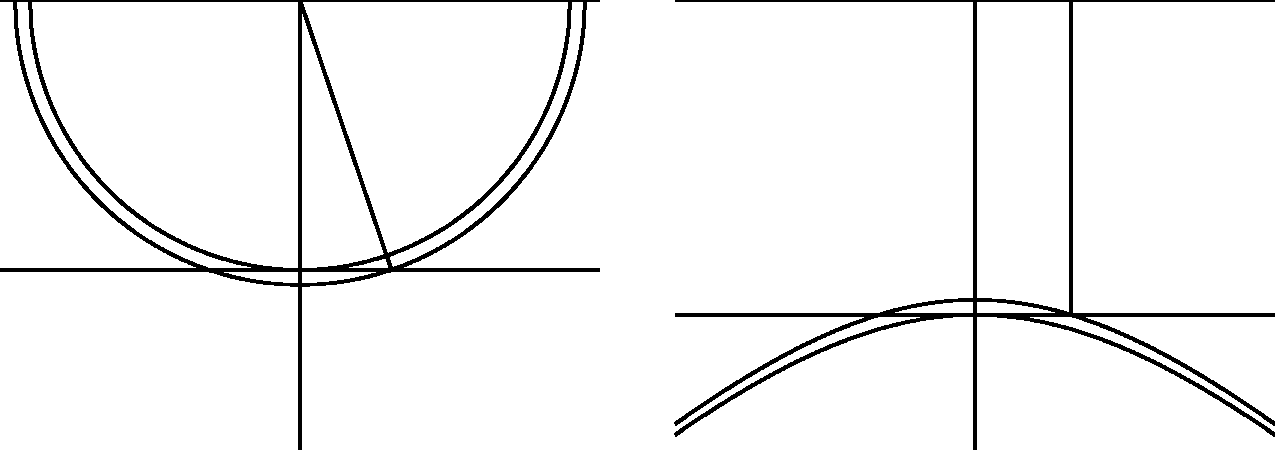
\includegraphics[width=0.95\textwidth]{omk/fresnel}
\caption[fresnel]{$(x,z)$空间内的菲涅尔带(左)及$(x,t)$空间内的菲涅尔带(右)}
\label{fig:omk/fresnel}
\end{figure}

波动传播相当于一种褶积滤波,从沿反射面分布的一个区域$\Delta x_{2}$(或地下一个
区域$\Delta x_{1}$)至地面上某一点这个范围内的信息,均受其影响。波动传播的逆过程
,即偏移,则相当于一种反褶积处理。横向分辨率的高低归根结底要查资料的空间频宽所限制。

即使是在反射面未表现出有倾角的地方可能还需有求于偏移。当要求必须在小于$\Delta x_{2}$
的精度范围之内来选定一个井位时,解释人员就得仔细检查振幅或波很沿反射面有何细微变化出现;
偏移使这些振幅变动与波形变动沿着反射面发生变化并有水平方向移动,所移动的距离就大约等于
菲涅尔带。

地震波速度随深度而增大是造成分辨率受限制的原因,这是反射地震学中的一项基本事实。由此
而出现:波越深地传播进入地层时,由于速度不断增大,它们的空间波长就越长。垂直分辨率
的情形简单说来就是这样:波长越长,分辨率就越低。水平分辨率的情形也类似,只不过水平
波长是在地表面上直接测定的。图\ref{fig:omk/hyp2}就是说明这种情形。图中所示是浅部散射
体和深部散射体形成的双曲面,浅部双曲线顶部到达时间早且有较陡渐近线,深部双曲线顶部到
达时间晚且有不太陡的渐近线。不太陡的渐近线有比比较长的水平波长,尽管速度随深度而增大,
地面上所测定的水平波长在同一深度并不改变(\ref{sec:1.5}节证明,这暗示着Snell定律)。
所以,横向空间分辨率随深度之增大而变坏。上述关于分辨率降低的原因综合起来,就可以解释
说明为什么在较晚的旅行时间上出现高频能量损耗。

\begin{figure}[H]
\centering
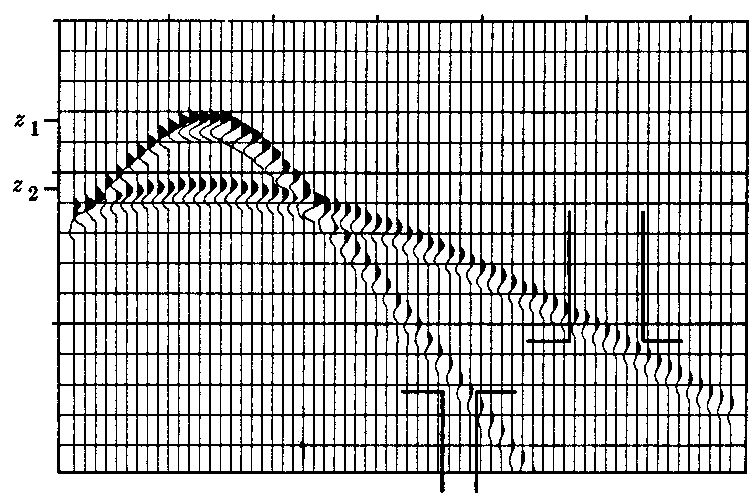
\includegraphics[width=0.65\textwidth]{omk/hyp2}
\caption[hyp2]{速度随深度而增大的地层所形成的双曲面。由图可观察到横向的波长随深度之增加而变得
更长,由此可知,横向分辨能力随深度之增加而降低}
\label{fig:omk/hyp2}
\end{figure}

\subsection{二维傅氏变换}
\label{sec:1.2.4}

在更深入一步讨论之前,且先回顾一下关于二维傅氏变换的若干基本事实。二维函数在计算机
内以矩阵内的数值代表。计算机内的一维傅氏变换是一种向量运算。二维傅氏变换可以采用一
系列一维傅氏变换来进行计算,你可首先变换矩阵的每一列向量,然后再变换矩阵的每一行向
量:换一种办法,先进行行向量后进行列向量的变换也行。用图形表示如下:

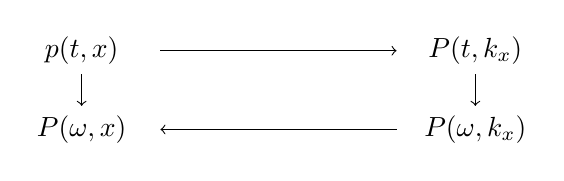
\begin{tikzpicture}
\draw[->] (11.0,1.5) -- (14,1.5);
\draw[<-] (11.0,0.5) -- (14,0.5);
\node at (10,0.5) {$P(\omega,x)$};
\node at (10,1.5) {$p(t,x)$};
\draw[->] (10,1.2) -- (10,0.8);
\draw[->] (15,1.2) -- (15,0.8);
\node at (15,0.5) {$P(\omega,k_{x})$};
\node at (15,1.5) {$P(t,k_{x})$};

\end{tikzpicture}

该图有个符号问题要注意,我们不能继续采用通常的符号约定:以小写字母代表物理空间
域,以大写字母代表傅氏变换域:因为那种约定不可能包括混合对象$P(t,k_{x})$和$P(\omega,x)$。
看来,与其是创造一些新符号,还不如最好是让读者利用该图所示上下关系去妥善处理这个
符号问题。函数的自变量必须有助于函数的命名,不要相混。

图\ref{fig:dft/plane4}所示是对典型的深海地震资料进行这些变换的一个例子。
\begin{figure}[H]
\centering
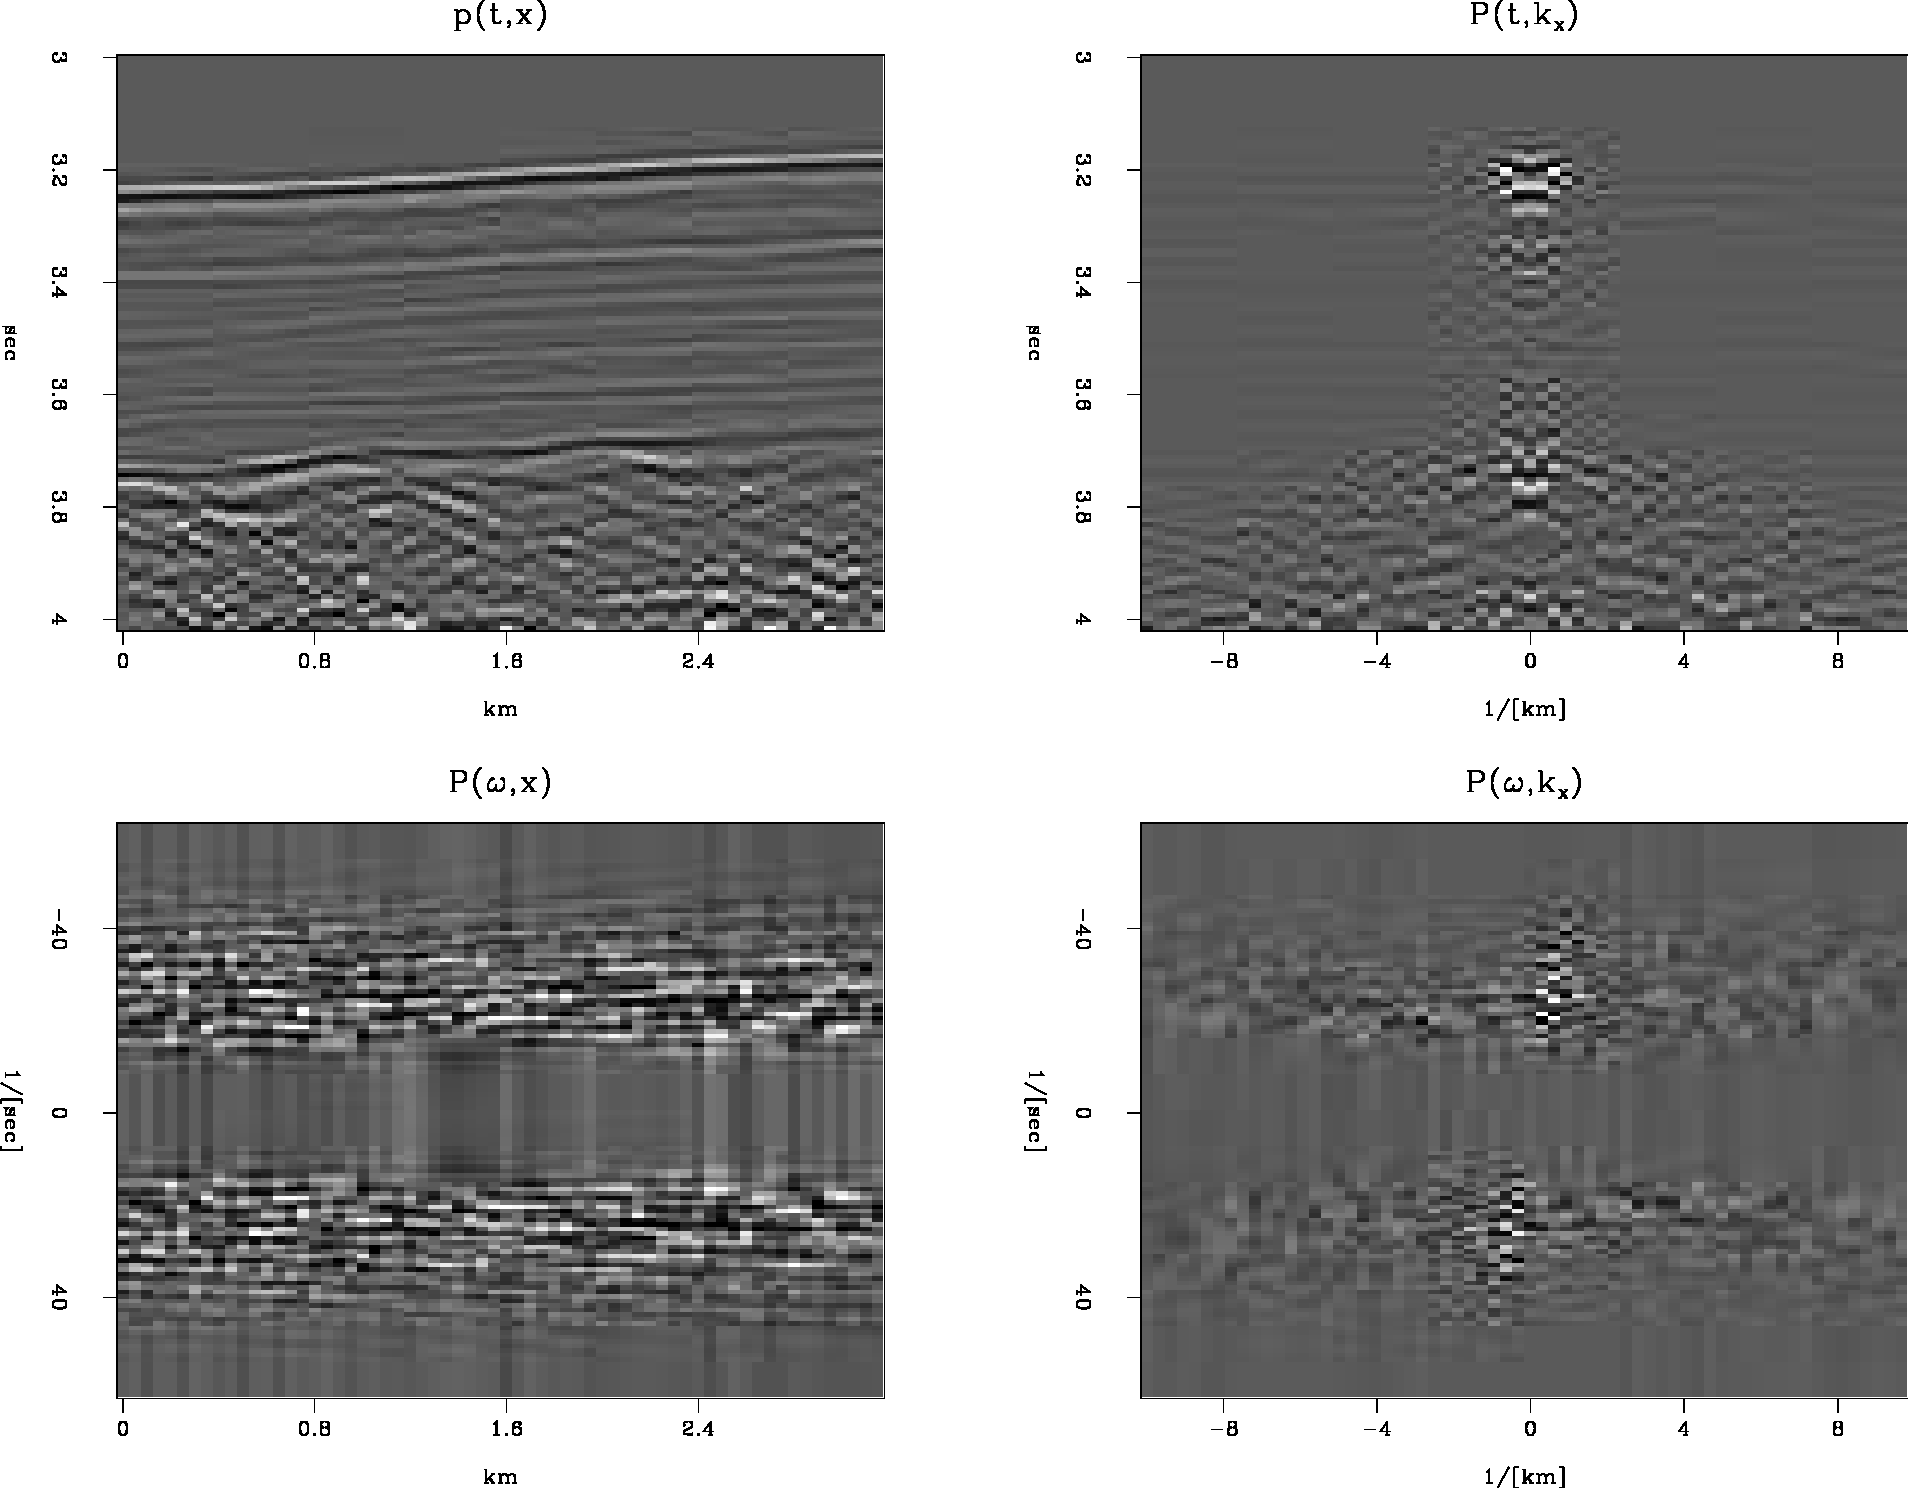
\includegraphics[width=0.95\textwidth]{dft/plane4}
\caption[plane4]{深海地震时间剖面$p(t,x)$及其各种傅氏变换的实部。由于通过水层
的旅行时太长,图中的时间轴未从$t=0$时开始}
\label{fig:dft/plane4}
\end{figure}

在深海,沉积物均属细粒并缓慢沉积为平缓而又规则的水平地层。缺少像砂岩那样的具
有渗透性的岩石,大大降低了从深海寻找石油的可能性。细粒页岩覆盖在不规则的基底
火成岩之上。在$P(t,k_{x})$的图中,低$k_{x}$值处有很强的谱,表示沉积地层具有横
向连续性;$k_{x}$的这种谱延伸至很大$k_{x}$值,致使深资料可能受到一点空间假频
影响(采样点过稀),这表示存在有火成岩。$P(\omega,x)$的图形表示该资料包含的不是
低频能量,能量在很大$\omega$时并不如所预料那样很快衰减,这表明存在有时间方面的
假频。在$p(t,x)$图形中,这种假频现象在阶梯状外形的海底初至中也是很明显的。倾斜
的海底在$(\omega,k_{x})$空间内表现为能量以某一种角度通过原点。

总而言之,一个地震记录集合的二维傅氏变换仅只涉及对每一地震记录进行两次一维傅
氏变换的计算,这是很幸运的事。为证实上述处理办法确实是实现二维傅氏变换,让我
们列出一些方程,首先说一下,任何$x$与$t$的函数均可表示为谐波函数之叠加和(傅
氏变换中采用的符号约定将在\ref{sec:1.6}节中解释),即
\begin{equation}
p(t,x) = \iint e^{-i\omega t+ik_{x}x}P(\omega,k_{x})d\omega dk_{x}
\label{eq:ex1.2.9}
\end{equation}
这种逆傅氏变换中的积分核具有波的形式——沿$x$轴的正方向传播的波。同样地,在正傅氏
变换中,为保持积分核是一个沿正方向传播的波,两个指数的符号均应改变。式中,为方便
起见,比例因子与无穷积分限均已略去。(离散计算时,积分限与比例因子均各不相同,何
必为此操心费事?)重积分可加括号,以表明要首先完成时间方面的变换
\begin{align*}
   & p(t,x) \notag \\
={}& \int e^{ik_{x}x}[\int e^{-i\omega t}P(\omega,k_{x})d\omega]dk_{x} \notag \\
={}& \int e^{ik_{x}x}P(t,k_{x})dk_{x} \notag
\end{align*}
括号内的量是就每个$k_{x}$完成的对$\omega$的傅氏变换。换一种方式也行,将$k_{x}$积分
放在括号内首先完成运算,那意味着首先完成行运算而不是列运算(或者反之)。正是函数$exp(-i\omega t+ik_{x}x)$
分离为两个指数之乘积的这种可分解性,才使进行这种重积分的计箅轻而易举而又节省时间。

\subsection{输入输出关系}
\label{sec:1.2.5}

将数据资料向下延拓是偏移过程的核心部分。已知在地表面$z=0$这个平面上的输入数据,
我们必须构制出在深度$z$上可被记录到的数据。这点在傅氏变换域内很容易做到,这种
方法可被看作是直接乘以某个复指数的乘法运算,即
\begin{equation}
P(\omega,k_{x},z) = P(\omega,k_{x},0)e^{ik_{z}(\omega,k_{x})z}
\label{eq:ex1.2.10}
\end{equation}
既然运算是傅氏变换域内的一种乘法,那就能够用图解方式描述它:

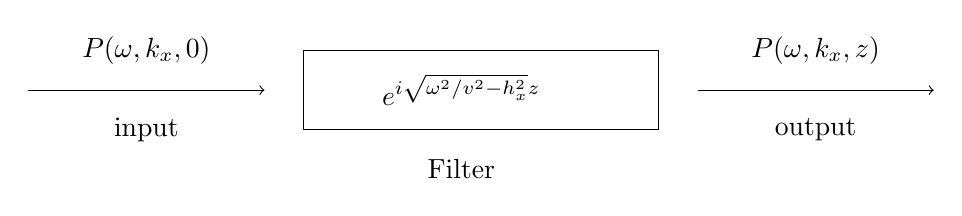
\begin{tikzpicture}
\centering
\draw[->] (2.0,1.5) -- (5.0,1.5);
\node at (3.5,2.0) {$P(\omega,k_{x},0)$};
\node at (3.5,1.0) {input};

\draw (5.5,1.0) rectangle(10,2.0);
\node at (7.5,1.5) {$e^{i\sqrt{\omega^{2}/v^{2}-h_{x}^{2}}z}$};
\node at (7.5,0.5) {Filter};

\draw[->] (10.5,1.5) -- (13.5,1.5);
\node at (12,2.0) {$P(\omega,k_{x},z)$};
\node at (12,1.0) {output};

\end{tikzpicture}

在频率$\omega$域内和波数$\k_{x}$域内,向下延拓都是一种乘积关系,那么该滤波器在
时间和空间域内看来又像是什么呢?原来它像是一神圆锥,粗略地说,这是$x^{2}+z^{2}-v^{2}t^{2}$
的一个脉冲函数;更精确地说,这是惠更斯二次波震源,前面曾经用海洋波浪通过防波堤
的一个空隙洞穴为例说明过它。将防波堤内多种多样空穴的响应相加起来,那就是遍及$x$
轴的褶积,将许多入射海波叠加起来,那就是遍及时间$t$的褶积。

现在让我们来看一下为何向下延拓滤波器会具有所述数学形式。$\omega,k_{x}$平面内的
每一点都与一正弦平面波有关,随深度而发生变化也将是正弦函数形式、即$exp(ik_{z}z)$,
对该正弦波而言,求解出方程$(8)$就可直接求出$k_{z}$的值:

\begin{subequations}\label{eq:ex1.2.11}
\begin{equation}
k_{z}=\pm(\frac{\omega^2}{v^2}-k_{x}^{2}) \label{eq:ex1.2.11a}
\end{equation}
\begin{equation}
 =\pm \frac{\omega}{v}(1-\frac{v^2k_{x}^{2}}{\omega^{2}})^{1/2} \label{eq:ex1.2.11b}
\end{equation}
\begin{equation}
 =\pm \frac{\omega}{v}cos\theta \label{eq:ex1.2.11c}
\end{equation}
\end{subequations}
选择正号意味着$exp(-i\omega t+ik_{z}z)$是一下行波(因为$z$随$t$之增大而增大时相位
将保持恒定);选择负号则形成一上行波。爆炸反射面概念要求有上行波,所以我们几乎总
是采用负号,不论我们是进行偏移还是进行摸拟。

取$e^{i\phi}$形式的输入输出滤波器看来是没有振幅比例因子的相移滤波器,这对我们计划进
行反褶积处理是一个好兆头,因为这意味着关于信噪比的顾虑,对于偏移处理要比对于普通
的滤波处理少得多了。

\subsection{习 题}
\label{sec:1.2.6}

\begin{enumerate}
\item
    假设你能在普通地震频率范围内观测到某些横波,请问空间分辨率较之通常情形
是好一些、是一样、还是变坏了?为什么?
\item
    试对本书中有关野外资料上的双曲线形初至浏览一下并测定其弗莱涅带宽度,在
没有零炮检距记录之处,有效的近似必须是沿一倾斜的直线测定${\Delta x_{2}}$
的大小。
\item
试对图\ref{fig:dft/plane4}中的$P(\omega,x)$图形内之水平“成层”现象作出解释。
该“层”之间距由什么决定?“层”的斜率由什么决定?
\item
试问日本海槽有多深(水层速度为1.5公里/秒)?
\item
    波场随时间的演交由下式描述
\begin{equation*}
p(x,z,t)=\iint[P(k_z,k_z,t=0)e^{-ix(k_x,k_z)}]e^{ik_xx+ik_zz}dk_xdk_x
\end{equation*}
设$P(k_x,k_z,0)$为常数,表示$(x,z)$空间中位于原点上的一个点源;令$t$非常大,意即被
积函数中的相位$\phi=[-\omega(k_x,k_z)+k_x(x/t)+k_z(z/t)]$是随$k_x$与$k_z$之变化而急
速改变。设仅当该相位为平稳相位时时,即$\partial\phi/\partial k_x$和$\partial\phi/\partial k_z$
均为零时,该相位才对积分有显著影响。试问同相轴位于$(x,z,t)$空间内何处?
\item 波场向下延拓以下式表示
\begin{equation*}
p(x,z,t)=\iint[P(k_z,z=0,\omega)e^{-ik_z(\omega,k_z)z}]e^{i\omega t+ik_xx}d\omega dk_x
\end{equation*}
设$P(k_x,0,\omega)$为常数,表示在空间内原点上的一个点源。试问同相轴应位于$(x,z,t)$
空间内何处?
\end{enumerate}

\section{四种广角偏移方法}
\label{sec:1.3}

本节所述反射地震资料的四种偏移方法均为现代生产环境中出现的方法。它们是易于处
理广角射线问题的一类方法,同时又是难以应用于处理速度横向变化问题的一类方法。

\subsection{旅行时间深度}
\label{sec:1.3.1}

偏移处理程序的输出,理想的应是$(x,t)$平面中的图像,可实际上垂直坐标轴几乎从
来不是深度$z$,而是垂直旅行时间$\tau$。在恒速地层情形下,该时间与该深度由一
个比例因子联系起来,比例因子的意义就是:与$(x,t)$平面相比$(x,\tau)$平面的垂
直比例放大了。在地震普查工作中,垂直方向往往放大五倍左右。到了业已充分缩小
勘探范围以便定井位的时候,采用的垂向放大比例因子很可能是1左右(即没有放大)。

旅行时间深度$\tau$的定义通常包括波下行传播和上行传播二者的时间,这相当于使岩
层速度隐含有因子2。地震时间剖面一般是按爆炸反射面波场解释的,为使之一致,在
波场分析时要使岩层速度$v_{true}$减半,即
  \begin{equation}
  \tau=\frac{2z}{v_{true}}=\frac{z}{v_{half}}
  \label{eq:ex1.3.1}
  \end{equation}
地震资料解释中的第一项任务就是计算出垂向放大的近似数值。这个数值恐怕不会打印
在数据说明中,因为速度还未真正已知。再者,速度通常随深度而增大,意昧着垂向放
大随深度而减小。对于速度分层介质,时深转换公式为
\begin{gather}
\tau(z)=\int_{0}^x\frac{dz}{v(z)} \notag \\ 
\frac{d\tau}{dz}=\frac{1}{v} \label{eq:ex1.3.2}
\end{gather}

\subsection{绕射扫描与等时线扫描}
\label{sec:1.3.2}

绕射扫描与等时线扫描\footnote{原文中的hyperbola-summation method
按国内现已熟悉通用的术语,译为绕射扫描,semicircle-super-position method
则译为等时线扫描。——译者}是所有已知方法中最易于理解的偏移方法。

$(x,z)$空间内的圆或$(x,t)$空间内的双曲线这类圆锥截面的方程为
\begin{subequations}
\begin{equation}
z^2+x^2=v^2t^2
\label{eq:ex1.3.3a}
\end{equation}

转换为旅行时间深度$\tau$时,则

\begin{equation}
\tau^2+\frac{x^2}{v^2}=t^2
\label{eq:ex1.3.3b}
\end{equation}
\end{subequations}
式中,$v$为速度。
图\ref{fig:omk/schneider}是等时线扫描方法的图解说明(图件及其标题说明均取自
Schneider的经典论文〔1971〕)。取数据场使之包含有少量几个脉冲函数时,输出应
是适当的一些半圆之叠加结果,各个半圆代表单个脉冲所形成的那种球形反射面地层模
型。取数据场为各具有一千个采样点的一千个地震记录道时,则输出就是一百万个半圆
的一种叠加结果。既然地震记录既有正极性又有负极性,于是半圆将半数是以负极性叠
加,最终叠加结果看起来差不多会很像个样子。确实,除了在$(x,\tau)$空间内的一个
孤立脉冲之外,各半圆几乎处处都可能彼此相互抵销。发生这事,你可能会正确地猜出:
$(x,t)$空间内的输入数据剖面就是一种惠更斯二次震源,即能量是沿一双曲线集中分布
的。这点将引导我们转向绕射扫描方法的讨论。

偏移的绕射扫描方法如图所示。方法的基本思想是要在$(x,\tau)$空间的某个时间上用
扫描办法形成一个点,而不是像等时线扫描方法那样,把一百万十半圆彼此叠加在一起
逐点形成$(x,\tau)$空间内的各个点。为在$(x,\tau)$空间的输出结果中形成一个固定
点,试想像有式\ref{eq:ex1.3.3b}所示的一种双曲线,使其顶部位于$(x,\tau)$空间的
相应位置上。把该双曲曲所接触到全部数据值相加起来,所产生的值就作为$(x,\tau)$
空间内适当位置上的输出结果。按同样方法将$(x,\tau)$空间内所有其他位置均填满。

\begin{figure}[H]
\centering
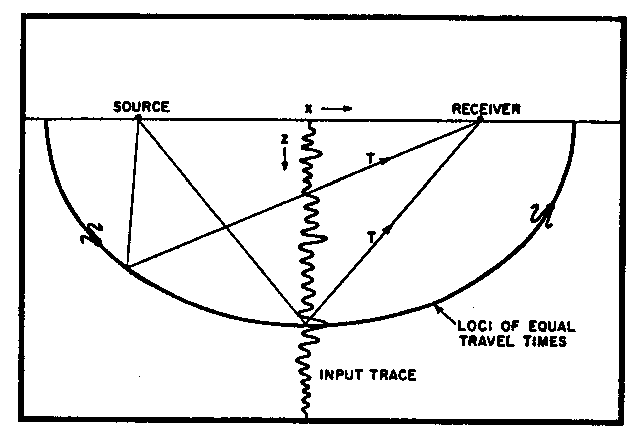
\includegraphics[width=0.5\textwidth]{omk/schneider}
\caption[schneider]{等时线扫描方法示意图。图中所示代表按炮检距中点位置的深度
(也可用时间)显示的一个输入记录道所发生的过程。将这个记录道各个振幅值沿一个曲
线分布,构制成地下界面,该曲线代表震源至反射点再至接收器的旅行时间为常数之各
点的轨迹。如速度为常数,则这些曲线是以踩源与接收点为焦点之椭圆。按这神处理办
法构成的图形,简单说就是以记录道振幅信息调制的波阵面图。它本身显然不是一个有
用的界面映像,但是当由相邻一些记录道(不同炮检距的共深度记录道)的类似图形构
制成图时,由于在古典的惠更斯原理意义上的波阵面之间发生相长干涉与相消干涉。就
产生了有意义的地下界面映像。例如,相邻记录道的波阵面会全部相交于一个绕射源上,
相长叠加而形成以强振幅斑点形式出现的一个绕射体映像,其垂向与水平方向的分辨率
由脉冲频宽及水平扫描半径所控制。另一方面,在有反射界面情形下。来自邻近记杂道
的波阵面均与该界面相切,从面由于相邻波阵面重叠部分的相长干涉而形成反射面映像。
在没有反射体与散射体之界面的区域内,波阵面由于随机叠加而趋于抵销}
\label{fig:omk/schneider}
\end{figure}
\begin{figure}[H]
\centering
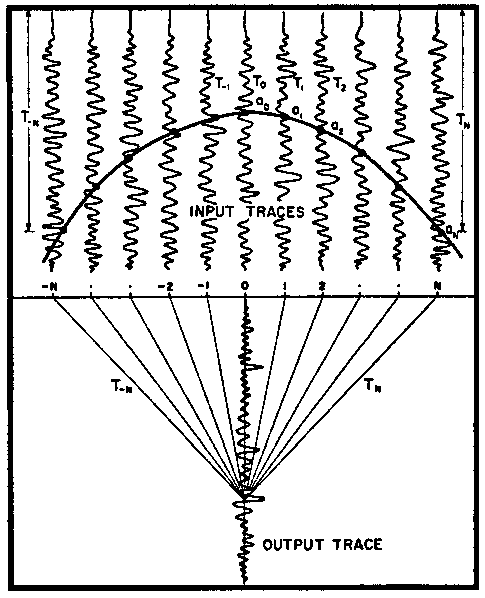
\includegraphics[width=0.5\textwidth]{omk/schneider2}
\caption[schneider2]{绕射扫描方法示意图。这个处理过程代表如何由图上部所示多次
叠加记录道组成的输入记录道集合产生出一个输出道记录道,图下部的输出记录道是反映
如何沿所示旅行时间曲线进行振幅求和而得出$(x,z)$点上的各个振幅值。这个曲线定义
为绕射双曲线。如果在所示输出点上的地下届面中存在有一个绕射源,则在该点将应形成
强振幅。这个过程也适用于反射面,因为一个反射面可以看成是连续的一系列绕射源,其
各自的映像合并产生一光滑连续分界面}
\label{fig:omk/schneider2}
\end{figure}

我们可以怀疑绕射扫描方法究竟是比等时线扫描方法好一点还是坏一点,或者它们是否
是等价的,相反的数据处理过程------或根据数据来建立模型——就是根据模型构制合成
记录。把以上所述两种偏移处理程序作一点改变,就可以变成模拟程序,这时,你不是
进行双曲线求和(译注:即绕射扫描hyperbola summation)或半圆叠加(译注:即等时
线扫描semicircle superposition),而是进行双曲线叠加(hyperbola superposition)
或半圆求和(semicircle summation)。我们也可以怀疑上述两种偏移处理程序是否真正
就是模拟程序的逆过程。有一些需要加以考虑的因素:
\begin{itemize}
\item 惠更斯二次震源波形振幅对角度的依从关系(即倾斜函数);
\item 能量所受球面发散影响;
\item 惠更斯二次震源波形所受相移影响。事实证明,即使将这些复杂因素忽略不计,
  所得处理结果还是相当好的。
\end{itemize}


随着其他一些偏移方法的发展,这些早期偏移方法的缺陷被了解得更为深入,并且发现
只要仔细处理,大部分缺陷是可以改正的。后期发展的一些偏移方法有一个好处,那就
是它们实现了真正的全通滤波(all-pass filter)。这样一类偏移方法保存了资料数据的
一般外貌,这点可以认为是由于恢复了沿双曲线积分所破坏了的高频成分。Trorey(
1970)与Hilterman(1970)利用Kirchhoff绕射积进行的工作导致了正演模拟程序,这项工作
成果终于提出了使绕射扫描方法与其他偏移方法能够符合一致(至少对于恒速情形是如此)
的定量手段(Schneider, 1977)。现今的用术语中将任何绕射扫描或等时线扫描方法都称作
Kirchhoff法,而严格地讲,Kirchhoff分仅能应用于恒定速度的情形。

\subsection{空间假频现象}
\label{sec:1.4}

空间假频现象意味着沿空间坐标轴的数据采样不足,这种困难如此普遍存在,所有偏移
方法都必须考虑它的影响。

数据应按每波长多于两个点进行采样;否则波至方向就变得难以捉摸。图\ref{fig:omk/alias}
所示是沿$x$轴采样密度不足的合成数据,你可看出,在高频和陡倾角时,假频问题变得
很严重了。
\begin{figure}[H]
\centering
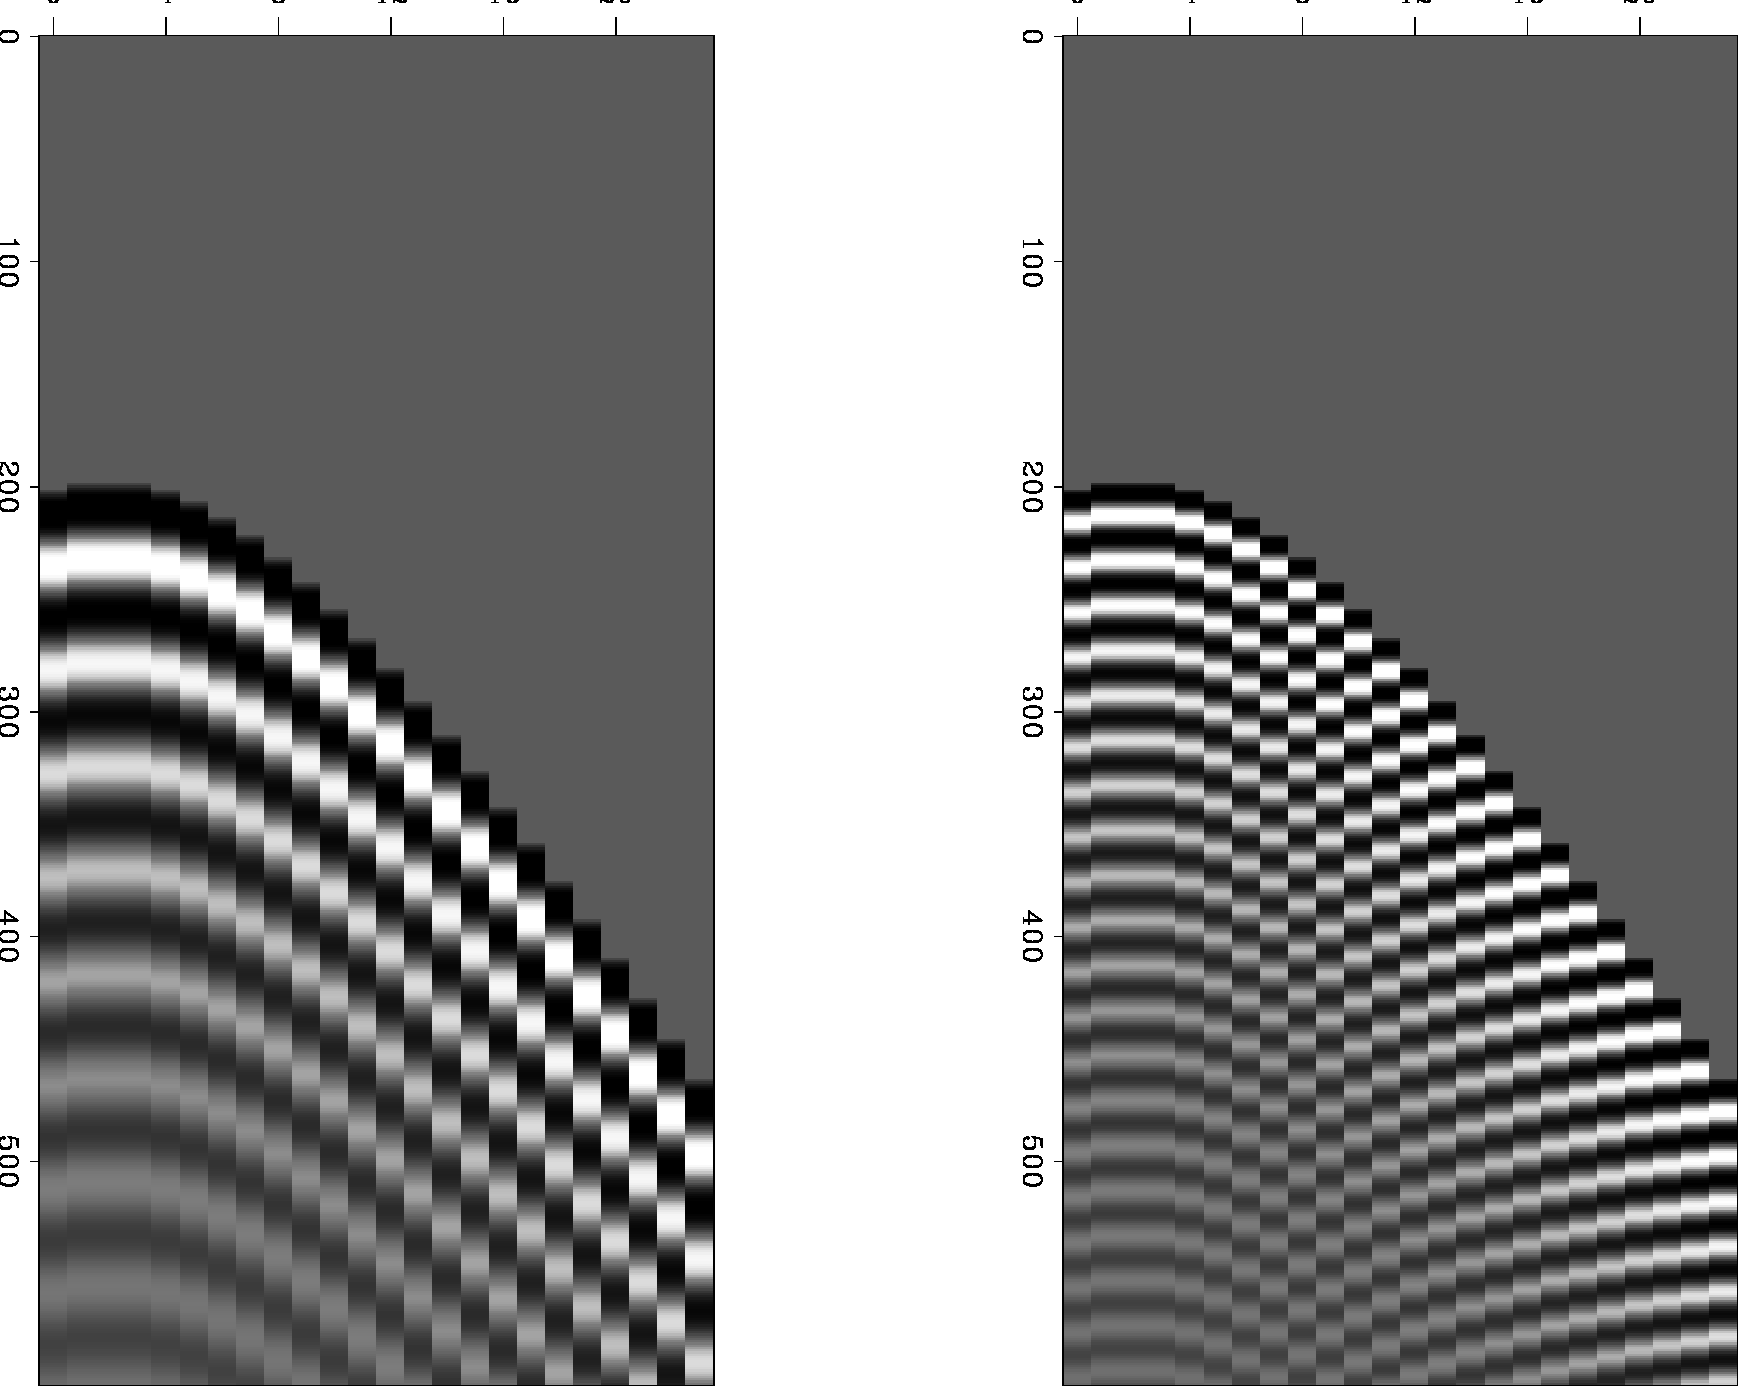
\includegraphics[width=0.95\textwidth]{omk/alias}
\caption[alias]{空间采样不足的合成数据。为更好地看出初至角度的模糊程度,
可从图侧以掠射角度来看}
\label{fig:omk/alias}
\end{figure}
对受空间假频影响的资料进行偏移,现在还没有什么普遍适用的可以自动校正其影响的
方法,在这类场合下,人可能比机器做得更好,因为人在识别真斜率时是很熟练的。然
而,当资料经过适当采样处理时,以波动方程为基飿的计算机偏移方法得出的结果还是
比人工方法强多了。当代地震勘探通常都是沿测线进行适当采样的,不过在垂直方向往
往存在困难。

各种绕射扫描型的偏算手苯5曼空间假频影响的危险,应该仔细处理以求避免这点。首
先要认识到,你应该沿双曲线的轨迹进行积分。每记录道只有一个采样点参与的求和过
程,是一种很粗略的近似,最好像图\ref{fig:omk/lineint}所示那样使更多采样点参
与求和。在双曲线呈陡倾斜之处,算子受假频影响的可能性就增大。在生产中,受假频
影响的算子往往是出现在海底反射之上,尽管海底可能是平坦的,可是由于双曲线的陡
倾斜翼穿过海底反射,于是算子在那里就获得了一种受干扰的外貌特征。
\begin{figure}[H]
\centering
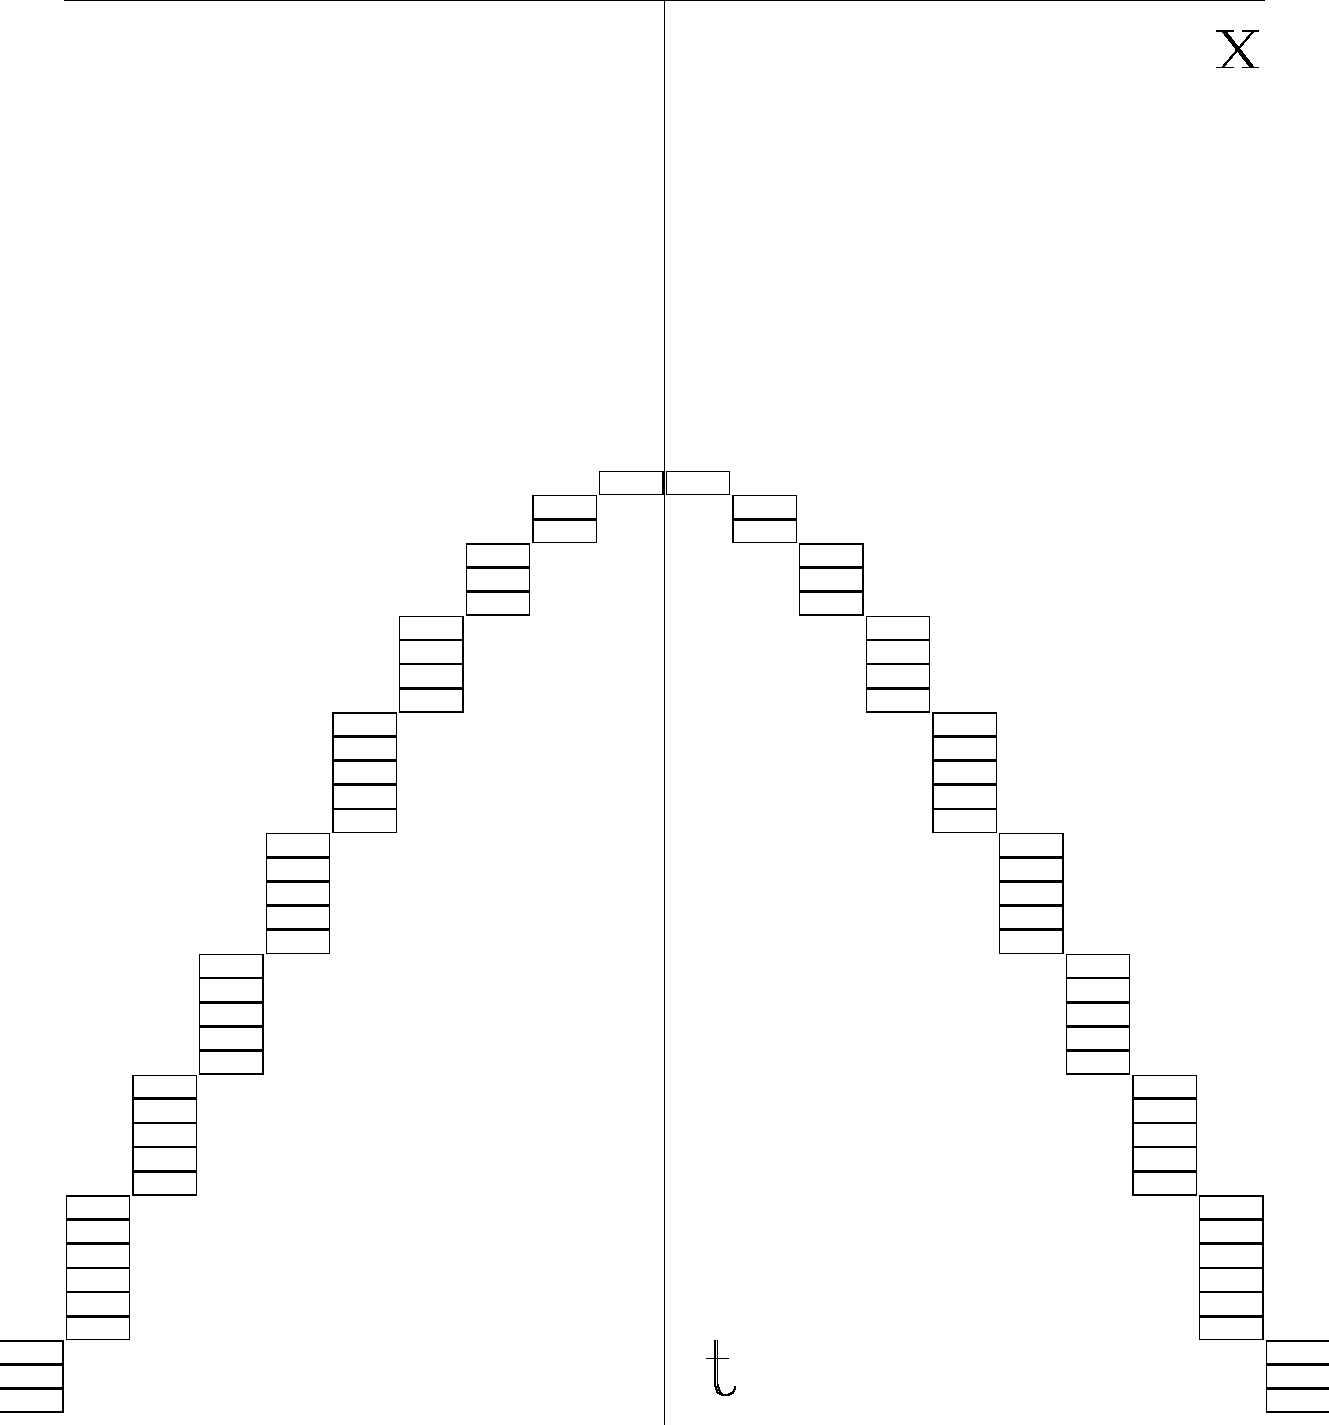
\includegraphics[width=0.6\textwidth]{omk/lineint}
\caption[lineint]{对于低速双曲线轨迹,积分将需要记录道多于一个采样点}
\label{fig:omk/lineint}
\end{figure}

\subsection{相移偏移方法(Gazdag法)}
\label{sec:1.5}

相移法用$\exp(ik_xz)$直接进行向下外推,然后估算$t=0$时(反射面在$t=0$时激发)的
波场。所有广角偏移方法中,属它最容易处理速度随深度变化的问题了,即使是相位角
和倾斜函数的影响,也都能正确地自动包括在内。同$Kirchhoff$偏移方法不一样,采用
这种相移法不存在使算子出现假频的危险。

相移法开始是对时间剖面进行二维傅氏变换(关于二维傅氏变换的某些实际细节,在1.7
节内讨论),然后把所有在$(\omega,k_x)$平面内的变换后的数据值乘以下式
\begin{equation}
e^{ik_z\Delta z}=exp\{-i\frac{\omega}{v}[1-(\frac{vk_x}{\omega})^2]^{1/2}\Delta z\}
\label{eq:ex1.3.4}
\end{equation}
向下延拓至某一个深度$\Delta z$。输出偏移剖面的时间采样间隔$\Delta\tau$通常选
择为等于输入数据的时间采样率(往往是4毫秒),所以,选取深度为$\Delta z=v\Delta\tau$
时,一个时间单位情形下的向下延拓算子为C,数据将多次乘以C,从而就是将它向下延拓
了许多$\Delta\tau$步长。
\begin{equation}
exp\{-i\omega\Delta\tau[1-(\frac{vk_x}{\omega})^2]^{1/2}\}=C
\label{eq:ex1.3.5}
\end{equation}
其次的任务是成像.在每个深度上完成一个逆傅氏变换之后,接着就选定其在$t=0$时的
值(反射面在$t=0$时激发)。很幸运,仅需在$t=0$时的一个点上完成傅氏变换,所以
这也就全部所需要的计算了。由于$t=0$时的值只是各个$\omega$频率分量之和,计算
特别容易(将$t=0$代入逆傅氏积分就可知道)。最后就是进行$k_x$至$x$的逆傅氏变
换。从上行波$u$计算出映像的偏移过程可以总结如下\footnote{关于RATFOR程序的说
明,见1.7节。括号符号${\ldots\ldots}$内为语句,符号$FT[\ldots\ldots]$表示对
符号$[\ldots\ldots]$内的函数完成傅氏变换。——译者}:\\
$U(\omega,k_x)$=FT[u(t,x)]\\
For $\tau=\Delta\tau,2\Delta\tau,\ldots\ldots$, end of time axis on seismogram\{\\
For all $k_x$ \{\\
 Image$(k_x,\tau)$ = 0.\\
		For all $\omega$ \{\\
			C = $exp(-i\omega\Delta\tau\sqrt{1-v^2k_x^2/\omega^2})$\\
			U$(\omega,k_x)$ = U$(\omega,k_x)$*C\\
			Image$(k_x,\tau)$=Image$(k_x,\tau)$+U$(\omega,k_x)$\\
		\}\\
	\}\\
	image$(x,\tau)$ = FT\{Image$(k_x,\tau)$\}\\
\}\\
逆偏移(即正演模拟)的处理与此非常箱似,从很大深度上其值为零的上行波开始,乘
以$exp(ik_x\Delta z)$,按步长将该波向上推进;随着通过地层的每个深度水平,由各
该深度水平上形成的爆炸反射面就不断加进上行波内。模拟上行波$u$的程序为:\\
$Image(k_x,z)$=FT[image(x,z)]\\
For all $\omega$ and all $k_x$\\
	U$(\omega,k_x)$=0.\\
For all $\omega$ \{\\
For all $k_x$\{\\
For z=$z_{max}, z_{max}-\Delta z, z_{max}-2\Delta z, \ldots\ldots, 0$\{\\
	C = $exp(+i\omega\Delta z\sqrt{v^{-2}-k_x^2/\omega^2})$\\
	U$(\omega,k_z)$ = U$(\omega,k_z)$*C+Image$(k_x,z)$\\
	\}\}\}\\
u(t,x) = FT\{U$(\omega,k_x)$\} \\
复指数内取正号是由于对上行波和向上外推需各取一次负号的综合结果;关于$\omega$
、$k_x$和$z$的三种循环是可互换的,当速度$v$是深度的一个恒定函数时,把复指数
$C$的计算移到关于$z$的内循环之外去进行,可以加快程序的运行。

速度很难总是精确已知,所以,尽管它可能是随深度而稳定増大的,但往往还是在一些
层内按常数来近似处理,而不是按地震记录上每一千个左右的时间点作缓慢改变。这种
近似处理的好处是节省计算的时间。式\ref{eq:ex1.3.5}内的平方根和正弦与余弦一旦
已计算出,就可以多次重复利用式$\ref{eq:ex1.3.5}$所示复数乘因子,采用4毫秒的
采样率和200毫秒的层厚,该复数乘因子能一直使用50次而后才放弃。

\subsection{Stolt方法}
\label{sec:1.3.6}

在大多数计算机上,Stolt偏移方法是有充裕余地的一种最快速的方法。就它的许多应
用而言,这点将是它最重要的特征。对于恒速地层情形,它是严格而又正确地同惠更
斯二次波源概念一致。像其他方法一样,这种偏移方法也可以使之颠倒而成为正演模
拟程序。有一个涉及原理问题的缺点,就是Stolt方法处理不了涉及速度随深度而变动
的问题。采用坐标轴拉伸处理(见4. 5节)来进行近似校正时种缺点就;能很大部分在
到补偿。还有一个实际应用上的问题,即所有傅氏变换都具有周期性。从原理上说,
这完全不成问题,因为在数据周围适当充填以零值就可以解决它。

Stolt方法可简单表示如下:\\
$p(x,t)\rightarrow P(k_x,\omega)\rightarrow(k_x,k_z=\sqrt{\omega^2/v^2-k_x^2})\rightarrow(x,z)$\\
现在看一看为什么要这样作.根据波场向下延拓的输入输出关系
\begin{equation}
P(\omega,k_x,z)=e^{ik_zz}P(\omega,k_x,z=0)
\label{eq:ex1.3.6}
\end{equation}
完成二维逆傅氏变换,得 \\
$P(t,x,z)=\iint e^{ik_xx-i\omega t+ik_zz}P(\omega,k_x,0)d\omega dk_x$\\
应用$(x,z)$点上的映像就是时间$t=0$时的爆炸反射面的这种思想,即得
\begin{equation}
Image(x,z)=\iint e^{ik_xx}e^{ik_z(\omega,k_x)z}P(\omega,k_x,0)d\omega dk_x
\label{eq:ex1.3.7}
\end{equation}
上式给出了最终的映像,但是它却是以一种不受欢迎的形式出现的。因为它暗示着必须
对每个深度$z$水平来完成一项二维积分。Stolt处理过程就是将如式\ref{eq:ex1.3.7}
所暗示的三维计算转换成一个二维傅氏变换。

到现在为止,还完全没有详细说明如何用上行波来代替下行波。波的方向是根据表达式
$exp(i\omega t+ik_zz)$中的相位保持恒定所要求的$z$与$t$之间的关系来定义
的,如$\omega$恒取正号,则$+k_z$将恒属于下行波而$-k_z$则恒属上行波。为描
述具有实值(而不是复数值)的波,既需要有正频率$\omega$也需要有负频率$-\omega$
,因此,下行波的固有特征就是$\omega$与$k_z$的符号必须一致,而上行波的固有特
征则相反。采用这种分类办法,把式\ref{eq:ex1.3.7}中的积分夺量从$\omega$改
变为$k_z$
\begin{subequations}\label{eq:ex1.3.8}
\begin{equation}
\omega=-sgn(k_z)v\sqrt{k_x^2+k_z^2} \label{eq:ex1.3.8a}\footnote
{$sgn(k_z)$表示$k_z$本身所取之符号。根据定义$\frac{\omega}{v}=k=\sqrt
{k_x^2+k_z^2}$,其中,$v$为速度;为使$\omega$的符号与$k_z$的符号相反,故
取此式.----译者}
\end{equation}
\begin{equation}
\frac{d\omega}{dk_z}=-sgn(k_z)v\frac{k_z}{\sqrt{k_x^2+k_z^2}} \label{eq:ex1.3.8b}
\end{equation}
\begin{equation}
=\frac{-v\mid k_z\mid}{\sqrt{k_x^2+k_z^2}} \label{eq:ex1.3.8c}
\end{equation}
\end{subequations}
将式\ref{eq:ex1.3.8}代入式\ref{eq:ex1.3.7}并在式中也包括该负号,因而像
对$\omega$的积分一样,对$k_z$的积分可取从负无限大至正无限大的积分限
\begin{equation}
Image(x,z)=\iint e^{ik_zz+ik_xx}\{P[\omega(k_x,k_z),k_x,0]\frac{v\mid k_z\mid}{k_x^2+k_z^2}\}dk_xdk_z
\label{eq:ex1.3.9}
\end{equation}
式\ref{eq:ex1.3.9}说明,所得映像是某种二维逆傅氐变换的结果。Stolt偏移方法
就是直接完成\ref{eq:ex1.3.9}的计算,算法步骤为:
\begin{enumerate}
\item 对资料进行双重傅氏变换,从$p(t,x,0)$变换为$P(\omega,k_x,0)$;
\item 在新网格上对$P$进行重采样,使它成为$k_x$与$k_z$的函数,并以比例因子
乘$P$(该比例因子可解释为$cos\theta$)\footnote{根据定义$k_z=kcos\theta$,
即$cos\theta=k_z/k=k_z/\sqrt{k_x^2+k_z^2}$,这时应将式\ref{eq:ex1.3.9}
中的速度$v$视为常数。由此可知,$cos\theta$即积分\ref{eq:ex1.3.9}中的乘因子。
——译者};
\item 进行逆傅氏变换,变换至$(x,z)$空间。
\end{enumerate}

脉冲应用Stolt偏移的实例如图\ref{fig:omk/stolt}所示。你可看到预期会有的半圆弧(
各个半圆孤的底部还挂着一个半圆弧,这些圆孤不但开口朝上、圆心位于地面$z=0$,而且开
口朝下,圆心位于底部位于最深位置的脉冲所形成之圆弧影响最大。众所周知,
更仔细地进行内插重采样就能压制掉这些圆弧(你把$\omega$的均勻网格转换为$k_z$的非
均匀网格就得采用内插方法),比方说,用$sinc$函数\footnote{sinc函数形式为$(sin u)/u$。
——译者}代替线性内插算子来进行内插就行(见4.5节)。避免弧形干扰的一种简单办法就是
干脆躲开该模型的底部,就是说,在底部充填许多零即可。
\begin{figure}[H]
\centering
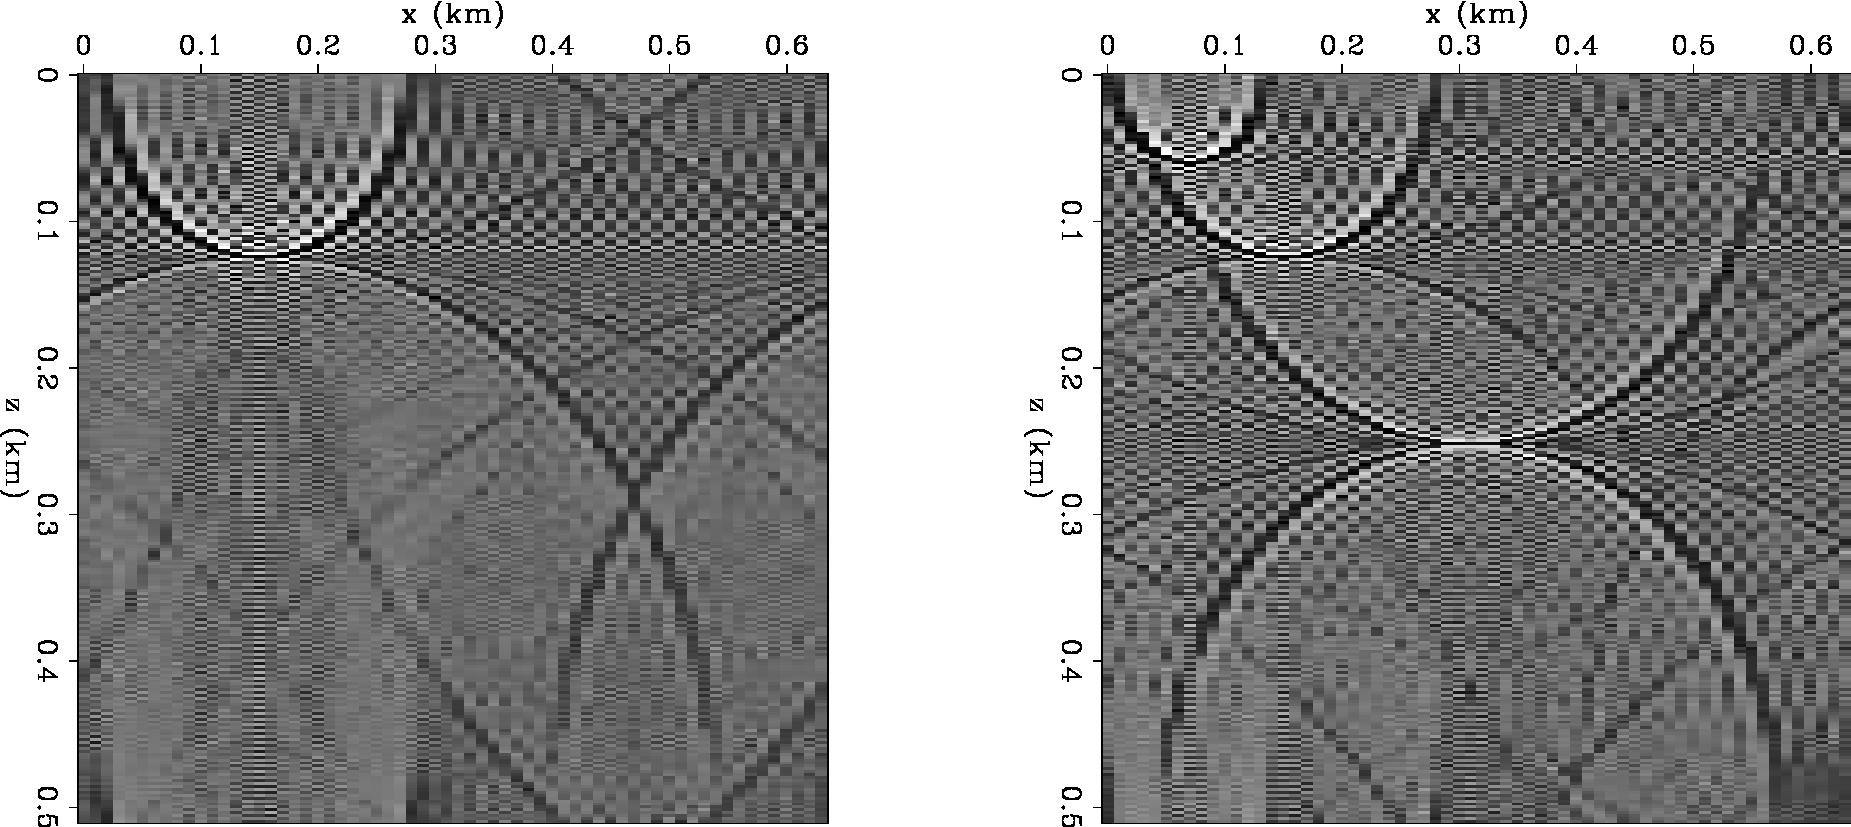
\includegraphics[width=0.95\textwidth]{omk/stolt}
\caption[stolt]{Stolt方法对脉冲数据的响应。可看到许多半圆弧与计算假象在一起}
\label{fig:omk/stolt}
\end{figure}
看来在时间轴上需要充填极其大量的零值,为保持合理的内存要求,可按习题(4)所
述算法重新加以组织。当然,$x$方向有周期性,所以沿$x$轴也需要充填零值。

\subsection{统射扫描法可改进为Kirchhoff法}
\label{sec:1.3.7}

Schneider ( 1978 )证明惠更斯二次震源子波的解析表达式为\footnote{$step(t-r/v)$
为阶跃函数。——译者}
\begin{equation}
FT^{-1}(e^{ik_zz})=\frac{1}{\pi}\frac{\partial}{\partial z_0}\frac{step(t-r/v)}{\sqrt{t^2-r^2/v^2}}
\label{eq:ex1.3.10}
\end{equation}
式中,$r$为震源(爆炸反射面)与接收器之间的距离$\sqrt{x^2+(z-z_0)^2}$。函数
\ref{eq:ex1.3.10}中含有一项极点和阶跃函数的导数,由于趋于无限大,实际上是不可能
用图形来表示这个子波函数的。不过,根据其数学形式,你立刻回认识到扰动全部集中于所
期望的圆锥面上。在该锥面上,阶跃函数之导数给出一个正脉冲初至,平方根倒数之导数给出
一脉冲,其负极性之尾巴以$-3/2$次幂阻尼衰减。因为导数是对$z$求导而不是对$r$求导,
所以会出现余弦倾斜因子。

式\ref{eq:ex1.3.10}说明的是二维惠更斯子波而不是三维子波(在次要的枝节方面有一些
不同),虽然点源产生的波主要是球面波,可是弯曲地层的聚焦作用却主要是一种二维聚焦,
亦即,弯曲地层不像是球面而倒更像是柱面。

你也许会奇怪:为什么严格的逆变换\ref{eq:ex1.3.10}虽已知而不论谁却还是宁愿采用它
的近似。实践证明,以图形表示式\ref{eq:ex1.3.10}的困难表现在用它对数据资料进行褶
积时有困难,那也正是为什么普遍公认前述一些Kirchhoff偏移方法在平缓海底反射之上要出
现前兆干扰。第二章和第四章的内容大部分是用于讨论将式\ref{eq:ex1.3.10}推广至变速
情形下也能成立,以及将它推广成为数据网格上比较好的表现形式。

在傅氏变换域内,惠更斯二次震源函数很简单而且足平滑的,在矩形网格上计算该函数然后采用
1.7节所述程序进行逆变换,是一桩简易的事,图\ref{fig:omk/huygens}所示是在一个
$256\times 64$网格点上的计算结果(在实际处理时,将采用大约是$1024\times 256$
的网格,但此处所采用之稀疏网格可提供一种具有适当细节的图形),因为以图形表示一个类似
于脉冲偶极子的函数有困难,在图\ref{fig:omk/huygens}的下部又显示了其时间积分的第
二种图形。
\begin{figure}[H]
\centering
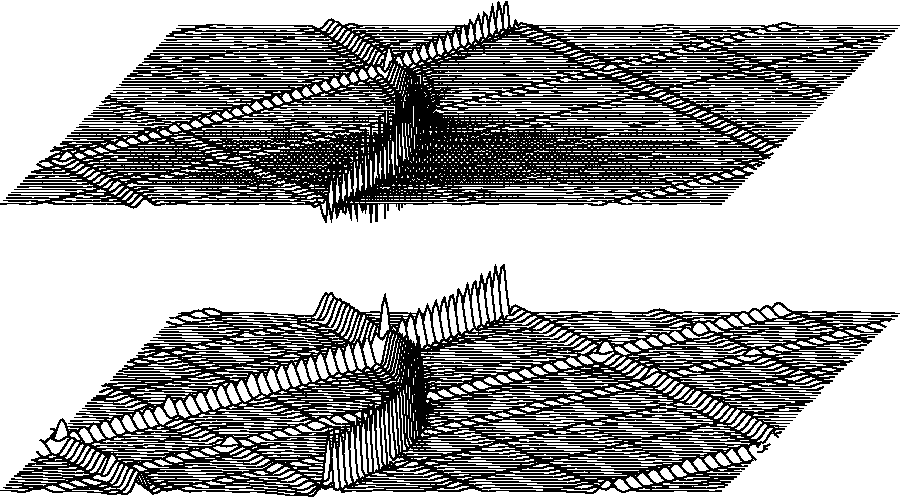
\includegraphics[width=0.95\textwidth]{omk/huygens}
\caption[huygens]{惠更斯子波(上图)及其平滑时间积分(下图)}
\label{fig:omk/huygens}
\end{figure}

\subsection{偏移方法对速度误差的灵敏度}
\label{sec:1.3.8}

图\ref{fig:omk/sensitive}表示偏移的脉冲响应随速度如何变化的情形。注意,偏移资料
通常是以时间剖面形式显示的,对于水平成层情形,任何速度误差都没什么影响\footnote{根
据能量耗散率常数$1/Q$的定义:\\
$\frac{\pi}{Q}=\frac{\alpha}{f}$\\
其中,$\alpha$为衰减系数,$f$为波的频率。因主周期$\Delta T$与频率之关系为$\Delta T = \frac{1}{f}$,
故得即比值$\frac{T}{\Delta T}=\frac{\alpha T}{\pi}Q$,即比值$\frac{T}{\Delta T}$
与$Q$值有关。——译者}。
\begin{figure}[H]
\centering
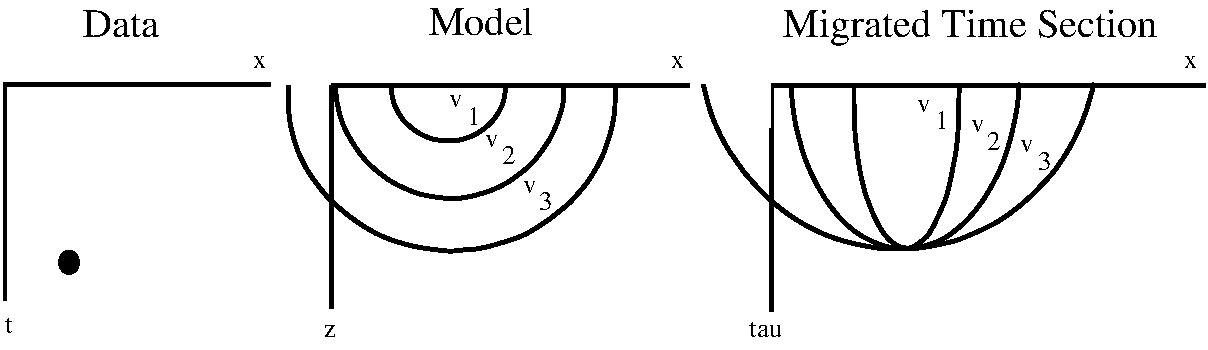
\includegraphics[width=0.95\textwidth]{omk/sensitive}
\caption[sensitive]{速度误差灵敏度随角度(可达$90^{\circ}$而增大。数据脉冲的偏移犹如是速度
之函数。三种可能的恒定速度选择均重叠显示在同一个平面上}
\label{fig:omk/sensitive}
\end{figure}
不同的人有不同的精确度准则,合理的准则应是:半圆弧上的能量之误差须小于半波长,对于沿
水平方向传播的能量来说,该项定位误差只与主周期$\Delta T$和旅行时间$T$有关\footnote{原文为“\ldots\ldots{}在间距是小于一个波长的情形下,\ldots\ldots”,显系有误。如杲确系小于一个波长,则需\\
$\Delta x=\frac{1}{2}Tsin\theta\Delta v<\lambda=v\Delta T$\\
从而\\
$\frac{\Delta v}{v}<\frac{2}{sin\theta}(\frac{\Delta T}{T})$\\
当$\theta=\pi/2$及$\Delta T/T=0.01$时,应有$\frac{\Delta v}{v}<2\frac{\Delta T}{T}=0.02$,
这个结果显然与$\theta=\pi/2$时“速度误差必须小于百分之一 ”的结论自相矛盾。由此可知,
所谓“小于一个波长”显然是“小于半个波长”之误。}。比值$\Delta T/T$超过$100$是难得见的,
看来这项数值$100$似乎是沉积岩的一种反射地震学基本观测参量(从理论上说,它也许与沉积岩的
“Q值”有关,或者,它可能与产生无序的层内多次反射有关系;在下列情形时出现高于100的大值:
(1)传播路程大部分均位于水层中时;(2)位于大于4秒左右的时间深度上时)。图\ref{fig:omk/senser}
是两种相近的偏移速度情形的比较,由图可知,两种曲线之间的间距随角度之增大而增大。在间距是小于半个
波长的。情形下,对于90°的角度,速度误差必须小于一百分之一;对于$45^{\circ}$倾角,偏移
速度误差可比它大$\sqrt{2}$倍\footnote{在偏移平面$(x,\tau)$内的等时线方程为\\
$\frac{4x^2}{v^2T^2}+\frac{\tau^2}{T^2}=1$\\
由此可得
$\tau=T\sqrt{1-\frac{4x^2}{v^2T^2}}=T\sqrt{1-sin^2\theta},x=\frac{1}{2}vTsin\theta (i)$
式中,$T$为双程传播时间,$\theta$为图\ref{fig:omk/senser}所示偏移方向与垂直方向之间的夹角。
根据定义(i),因速度$v$有误差$\Delta v$而形成之定时误差$\Delta \tau$与定位误差$\Delta x$
为\\
$\Delta \tau=T(\frac{4x^2\Delta v}{v^3T^2}/\sqrt{1-\frac{4x^2}{v^2T^2}})=T
sin\theta tan\theta(\frac{\Delta v}{v})$\\
$\Delta x = \frac{1}{2}Tsin\theta\Delta v$\\
或者\\
$\frac{\Delta\tau}{T}=sin\theta tan\theta(\frac{\Delta v}{v}) (ii)$\\
$\frac{\Delta x}{vT}=\frac{1}{2}sin\theta(\frac{\Delta v}{v}) (iii)$\\
由此可知:
\begin{enumerate}
\item 相对定时误差$\Delta \tau/T$与相对定位误差$\Delta x/vT$对相对速度误差$\Delta v/v$之灵敏度分别为$sin\theta tan\theta$与$(sin\theta)/2$,二者均随角$\theta$之增大而增大;
\item 对于固定的速度误差定时误差$\Delta v/v$随角度$\theta$之增大而增大;
\item 对于水平成层情形$\theta=0$,因$\Delta\tau=0$及$\Delta x=0$,从而既无定时误差亦无定位误差。
设$\lambda$为波长,$\Delta T$为主周期,即$\lambda=*v\Delta T$。若定位误差$\Delta x$小于半波长,即\\
$\frac{1}{2}Tsin\theta\Delta v<\frac{\lambda}{2}=\frac{1}{2}v\Delta T$,则\\
$\frac{\Delta v}{v}<\frac{1}{sin\theta}(\frac{\Delta T}{T} ) (iv)$\\
由式(iv)又可得结论:
\begin{enumerate}
\item 对于沿水平方向$\theta=\pi/2$传播的能量,应有\\
$\frac{\Delta v}{v}<\frac{1}{sin(\frac{\pi}{2})}(\frac{\Delta T}{T})=\frac{\Delta T}{T}$\\
亦即$\theta=\pi/2$时的速度误差$\Delta \theta=\pi/2$仅与主周期$\Delta T$和旅行时间$T$有关;
\item   $\Delta T/T$值一般为0.01,因此,在$\theta=\pi/2$的情形下,相对速度误差$\Delta v/v$必须小于0.01;
\item   由式(iv)可知,当$\theta=\pi/4$时,应有$\frac{\Delta v}{v}<\sqrt{2\frac{\Delta T}{T}}$,亦即$\theta=\pi/4$时的速度误差可比$\theta=\pi/2$时的速度误差大$\sqrt{2}$倍。——译者
\end{enumerate}
\end{enumerate}
}。
\begin{figure}[H]
\centering
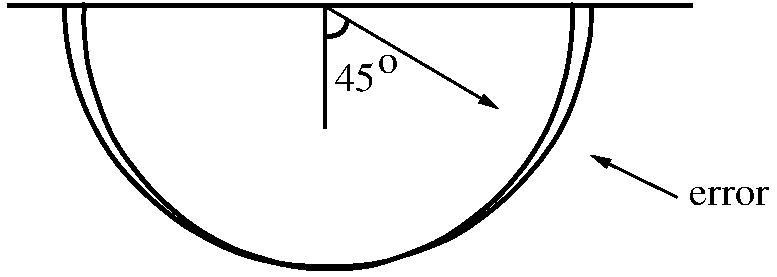
\includegraphics[width=0.6\textwidth]{omk/senser}
\caption[senser]{速度错误时的定位误差随角度而增大}
\label{fig:omk/senser}
\end{figure}

速度极少可精确已知到这神程度,所以我们可以怀疑广角偏移的价值。

\subsection{各种方法之比较与评价 }
\label{sec:1.3.9}

本节所述偏移的三种方法,比较如下:
\newcolumntype{Y}{>{\centering\arraybackslash}X}
\begin{table}[!ht]
\centering
\ttfamily
\small
\begin{tabularx}{\textwidth}{Y|Y|Y|Y}
%\begin{tabular}{p{3cm}p{4cm}p{4cm}p{5cm}}
%\toprule
\hline
 & 绕射扫描与等时线扫描法 & 相移法 & Stolt 法\\
%\midrule
\hline
运算速度 &慢 & 中等 & 极快\\ \hline
内存分配组织 & 不方便 & 良好 & 良好\\ \hline
垂向速度$v(z)$ & 采用射线追踪法& 易处理 & 采用拉伸方法近似处理\\ \hline
广角偏移有何问题? & 谨防数据假频与
					算子假频
 & 谨防数据假频 & 谨防数据假颏\\ \hline
是否需相位校正与
倾斜校正?
 & 在恒速情形下,可能
需作一些努力
 & 对任何$v(z)$均易于处理 &
在恒速情形下须作校正\\ \hline
有无$f-k$域假频干扰? & 无 & 在X轴上有干扰,减弱$t$
轴上干扰的方法见4.5节 &
在$x$轴上有干扰,减弱$(t,z)$
中的干扰的方法见4.5节\\ \hline
水平速度$v(x)$
 & 可使生产程序存在
严重的隐患
 & 可用迭代法与内插
方法近似处理 &
尚无已知的程序可处理\\ \hline
能否消除边界影响与不
规则采样间隔影响? & 极佳 & 差 & 差\\ \hline
%\bottomrule
\end{tabularx}
%\end{tabular}
\end{table}

展望以后几章的内容有可能对做为一类方法的各种广角偏移的质量作些注记,现在就作
一点评论将是有帮助的.这类方法最大的弱点就是它们难以处理横向速度变动问题;它
们的最大优点是处理广角的能力,但是却被数据采集与处理中其他环节的弱点所削弱。
这些弱点即:
\begin{enumerate}
\item   炮检距所张角度往往很大,而各种方法却均忽略了它的影响.CDP叠加剖面并非
  零炮检距剖面;
\item 甚至连垂直于测线方向的微小倾角都是忽略不计时,何必再去处理沿测线方向见
到的非常大的广角呢\footnote{意即垂直于测线方向的倾角对沿测线走向的视倾角有很
大影响,而前者在处理中常被忽略不计。——译者}
\item 数据总是采样密度不够,不足以代表陡倾斜资料而又无假频现象;
\item 速度资料的精度低,极难证明对广角进行处理的正确性;
\item 噪音干扰可能会压制掉所有回声反射,而这也就意味着存在有-种截止倾角了。
例如,试想像在两秒的时间深度上有含油储层,该处的数据记录则停止在四秒的时间
上,这意味着倾角在60°时就截止了\footnote{偏移时间剖面为$(x,\tau)$平面,未
偏移时间剖面为$(x,T)$平面,时间剖面上的时间深度为相应的偏移时间深度为$T$,二
者存在下列关系:$\tau=Tcos\theta$,其中,$\theta$为偏移角度,当$\tau=2$秒,
$T=4$秒时,应得$\theta=\pi/3$。——译者}。
\end{enumerate}
\subsection{习题}
\begin{enumerate}
\item 波动模拟程序流程简图均假设爆炸反射面为时间的脉冲函数,试修改程序流程简
图使波动模拟能包括一项震源波形$s(t)$
\item 偏移程序流程简图允许速度随深度而变化,然而当速度是恒定的深度函数时却可
相当快地提高程序的运算效率,试证明如何可作到这一点。
\item 试作出Stolt算法逆过程的程序流程——就是说,根据一已知模型作出合成记录。
\item Stolt算法可加以重新组织,使得沿$x$轴充零时所需要的内存得以减少。首先沿$x$轴
  进行傅氏变换,变换至$k_x$域,然后从数据所在$(t,k_x)$平面选择恒定$k_x$值的向量;可将每
  个向量移至某一长向量的空间内,然后进行充零和内插。试作出所述程序的流程图。
\item 已知地震资料是在四秒处截止,试问可观测到80°倾角的最深旅行时间深度是多少?
\end{enumerate}

\section{物理基础}
以前数节已讨论过波传播的几何地震学方面的问题,以及它们如何与地震成像有关,现
在我们将考虑其物理方面的问题如何与成像有关.传播介质具有质量密度和可压缩性,讨论
波动要考虑物质的加速度向量和压力梯度.静形变、地滚波、剪切、刚性、能量耗散、成层
沉积——像这样一些因素,与映像的构制有什么关系呢?

因为沉积岩的复杂性,应采用何种数学描述的问题还没有普遍一致的意见。为帮助你认
识起指导作用的理论可以作到什么程度,我将指出理论与现代工业实践之间的一些不一致之
处。

\subsection{碎屑岩沉积剖面}
一般而言,大多数储油岩石都是砂岩-砂岩往往是由水速不足以起搬运作用时在河口附近
沉积的沙所形成。在河口,可发现沙是沿着沙是沿着沙坝的末端沉积下来的,且往往大约为
$25^{\circ}$左右的坡度沉积。如图\ref{fig:xrf/river}所示。尽管沙并非沉积
于平坦地层内,但上述沉积过程却可以形成一种水平地层。
\begin{figure}[H]
\centering
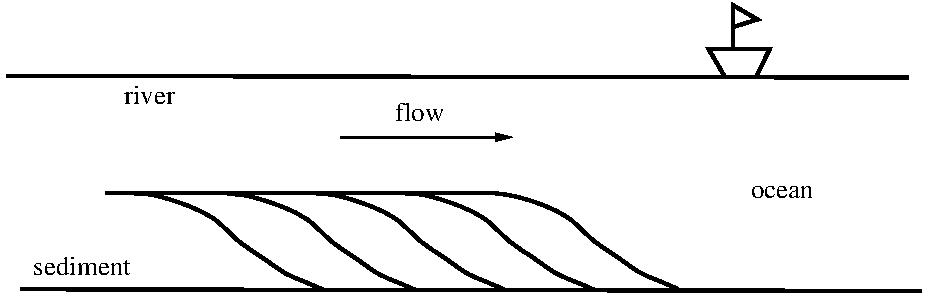
\includegraphics[width=0.5\textwidth]{xrf/river}
\caption[river]{河流入海处相当陡之斜坡上的砂岩沉积(储油岩石)}
\label{fig:xrf/river}
\end{figure}
粘土是甚细粒物质(杂质),在它们沉降而形成页岩之前,被携运至深水区域。页岩沉积
是比砂岩更为水平的一种成层地层。砂岩沉积的具体位置随经过之风暴和季节而变化,在
岩石中留下如木纹年轮状的标记。

由于河道与沙坝经常变化,河流三角洲本身就是一种复杂的沉积,它总是沿着海岸线移
动;在任何一个时期,三角洲似乎都是遗留下沉积物而向海洋方向移动,但是随后发生的沉
降挤压或者海平面升高又可引起它向陆地方向移动。


砂岩很重要,因为它的孔隙能使石油聚集,而它的渗透性能为石油运移形成通道。页岩
也很重要,因为它含有以前时期地球上的生物残迹并因而形成烃类.烃类运移至邻近的砂
岩,但总是不会运移至地面,因为砂岩为无渗透性的页岩所覆盖.尽管页岩具有比砂岩稍微
低一些的速度,可砂岩与页岩的波阻抗性质往往是类似的。地球物理学家要在地面上根据地
震波长的尺度(约30米左右)来观察这最终形成互层的砂页岩三维体。

砂岩页岩混合体称为碎屑岩、碎屑这个词的意是破碎。碎屑岩由结晶岩石的碎片所组
成,多数沉积岩均属碎屑岩,大多数石油是在碎肩岩内发现的,但在与碳酸盐岩有关的岩石
(如灰岩)中也发现了很多石油。碳酸盐岩是在浅海沉积环境由海洋有机物质所形成,许多
碳酸盐岩(及碎屑岩)由于缺乏渗透性而使所含石油难以抽取。经历若干还不太清楚的过程
之后,碳酸盐岩具有了渗透性。地震学家都知道碳酸盐岩具有的速度比碎屑岩速度要大,典型
情形是碳酸盐岩具有比邻近碎屑岩速度太20\%至50\%的速度。碎屑岩有时也包含有灰岩,在
这种情形下,称它为泥灰岩。

\subsection{年代地层学}
看来可能有点奇怪,关于地震反射的准确性质一直没有普遍一致的意见。物理学家倾向
于认为反射是由不同类型岩石的分界面、诸如砂页岩接触面所引起的。这种观在的麻烦
问题是:砂岩与页岩以复杂的方式形成夹层,既可大于也可小于地震波长。许多地质学家,
特别是以地震地层学家而知名的一群地质学家,他们有一种不同的概念(见美国石油地质学
家协会第26号研究报告:地震地层学一在油气勘探中的应用),他们曾经研究过成千英里
的具有测井资料的反射资料,相信一个反射是标志着一个恒定地质年代的地层。他们证实一
个连续追踪很长的反射面可以在一段是代表陆源沉积而另一端则是代表海相沉积,二者之
间可以有各式各样的岩石类型建立。在这种假说基础上的资料解释方法就称作年代地层学。
在整个全是碎肩岩沉积的地区震池层学家的观点看来是相当正确的。但是当存在有碳酸
盐岩和其它岩石时,物理学家的点看来要更为适宜,要进一步详细研究,建议读者读一读
Sheriff (1980)所著的书。

\subsection{转换横波难以观测}
在夭然地震学和实验室观测中,可清楚地观察到存在两种波速,速度较快者为压力波
(P波)而速度较慢者为横波(S波)。横波可随水平平面内的地面运动而呈极化(SH
波),或者在垂直平面内极化波)。理论、野外资料及实验室测定等结果均符合一
致。Cherify与Waters(1968)以及Erickson, Miller与Waters等人(1968
)曾经成功地在勘探环境条件下采用S波进行了试验工作。

值得注意的是,99\%以上的石油勘探工作均忽略了横波之存在。在数学上,是把地层当
作是一种流体或一种气体来进行处理的。横波试验工作采用专用设备来产生和记录垂直于测
线方向的振动、即SH波。由这些横波得出的地层图像往往为土壤层所削弱,但有时SH波
图像却清晰而一致。奇怪的是,纵使是良好的SH波资料也总是难于与P波图像对比。这些
试验研究表明,除了在土壤层中之外,典型情形下的横波传播速度大约为压力波的二分之
一,而在土壤层中,横波速度总是慢得多而且变动更大。观测到的横波通常具有比压力波低
的频率,其频率与速度均为压力波之二分之一的一种横波应正好具有与压力波相同的波长,
从而也就应具有与压力波相同的分辨能力。试验工作确实证明,横波可提供大约与压力波相
同的空间分辨能力,大多数地面地震资料只表示运动的垂直分量,而所有海上地震资料则是
记录压力波,所以,在常规的观测排列情形下,我们理应从来观察不到波,更精确地
说,SH波应很微弱,仅仅是由地层偏离简单的成层情形所形成。

反射地震学中有关横波的令人费解之问题是:石油勘探人员采用标准的野外观测系统按
常规方法观测由$P$波至$S$波的转换,这种企图失败了;而理论却预言以某种角度入射
在分界面上的$P$波应局部转换成$SV$波。再者,在通常所遇到的以$30^{\circ}$至
$60^{\circ}$角度入射的反射波这种情形下,这些转换波具有可与$P$波相比拟的强弱
范围。

常规的观测排列和处理在某种程度上是要削弱转换横波的,但是它也削弱多次反射(处
理方式非常相同),而我们是随时都可遇到多次波的。再者,转换波的波形特征类似于多次
波,可是二者是显著不同的两种波。转换波通常在速度测定中应有所显示(见第三章),图
\ref{fig:xrf/africa}所示是一种含有某些多次反射的零炮检距剖面,多次反射很容易
识别出来,因为它同较浅深度的地形模样完全相同。转换波将重复这种地形模样但时间标度
比例将穴约是3/2而不会严格等于4/2。在具有一种像图\ref{fig:xrf/africa}所示的
充分复杂的地形条件下,把转换波误认为是另一种一次反射的可能性将是很低的。
\begin{figure}[H]
\centering
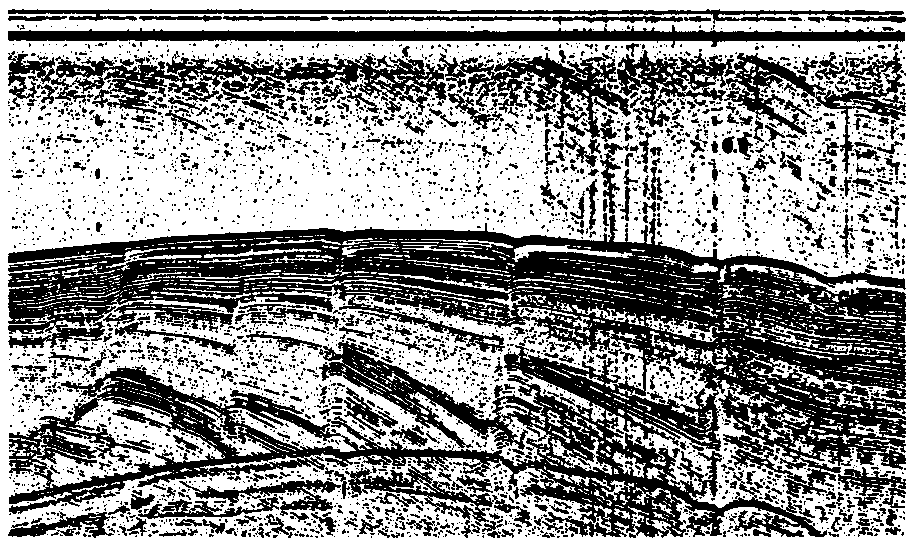
\includegraphics[width=0.5\textwidth]{xrf/africa}
\caption[africa]{东非地区带有多次反射的零炮检距剖面}
\label{fig:xrf/africa}
\end{figure}
在勘探中,转换波理应具有良好的判断价值,不过,在常规资料中观察出转换波的可能
性看来还相当渺茫,以致大多数解释人员都放弃了这种打箅。为什么在常规资料中观察不出
转换波?可以列举出若干理由:
\begin{enumerate}
\item
  在海上地震勘探资料中,因传播路径经过海水层,必然再度转换为$P$波;
\item
  在陆地资料中,表层土壤特别易于吸收横波能量;
\item 垂直分量检波器利于观测$P$波不利于观测$S$波,在近地表处因射线趋宁垂直,尤其
是如此。
\end{enumerate}

上述转换波为何会弱于压力波的所有理由中,没有一个是占有优势地位的。在广泛变化
的环境内记录到范围广泛的振幅,记录数据总是采用自动增益控制(AGC)加以显示,弱
振幅似乎尚不足以引致观测失败。关于这个问题,我们应继续注意研究,转换波应用于解释
无疑会比我们所承认的更为盛行(我还从未在常规记录上识别出转换横波)。

所以,虽然转换横波某天在反射地震学中起一种重要作用,可我们现在最好还
是转向讨论主流问题吧——如何有效处理常规观测的资料。

\subsection{混响模拟的可靠性}
地震学文献包括有大量关于成层介质内的地震波理论的讨论,应用地震学的一个值得注
意的问题是:一般均将层间内部的混响忽略不计。当波从一个分界面反射时,反射波强度只
等于入射波强度很小的一部分,典型的是小于10\%,这种反射波就是本书主要讨论的一种
波,然而,反射波本身还会反射而又反射,直至反射无限多次。对于短路程情形,可以有非
常多这样的射线。问题是这些混响是否总能累积达到足以值得去考虑它们的程度。看来答案
就是:这类混响虽可能有意义,可是地震学家很少能够用这种具体体现混响的相当复杂的理
论来改善反射地震勘探资料的解释工作。若干更详尽一些的讨论,可阅读5.5节。

当有测井记录可资利用,情况会有些改进,不过,这时也还存在有严重的困难。
处理之后最可能获得的横向分辨率大约为20米至50米,然而,测井记录并不是一种具有20米
呈50米数量级横向分辨水平的地层。你若观察过一个由高速公路切割出来的沉积剖面就会懂
得,一个点和一种横跨20至50米范围的横向水平之间是有很大差别的。在实际应用中,人们
都要对测井记录进行垂向平滑处理,过小的平滑会得出过多的混响,过多的平滑又会得不出
混响。垂向平滑的数量级是一个靠经验决定的参量,它对所得结果有显著影响。对测井记录
进行垂向平均不一定能满意地趋近所平分辨率。

\subsection{牛顿粘滞性理论的失败}
同样值得注意的问题是:地震学基本教科书在解释能量耗散参量Q值的频率依从关系时
遇到失败。关于能量耗散问题,最简单的理论处理办法必须对阐述应力与应变关系的胡克定
律加上一顼应变率。这种理论预言:高频能量相对耗散应比低频能量相对耗散强一些。可是
实验上观测到的却是:在几十赫兹频率范围上,相对能量耗散大略是恒定的。另一些简单的
牛顿理论则以$-i\omega$的多项式比值来描述应力与应变之比,这些理论均包含宥比例
长度及特征频率。它们都未预言Q值为常数。看来,一切比例尺度的岩石不均勻性似乎应该
成为一种成功的理论所应包括的本质属性(4.6节讨论的即属此种情形)。

\subsection{反演问题基本特点}

物理过程经常可用计算机按其自然面目进行模拟,计算机内存犹如是物理空间的图形,
而计算中的时间发展演化则犹如是所模拟的现实世界中的时间过程。按这种方式求解问题有
一个好处,就是没有任何关于解的唯一性的疑问,原始数据与模型离散化的误差不太可能造
成灾难性的影响。可是,勘探地球物理学家极少求解这类问题。我们通常不是把$(x,z)$空
间放在计算机内存中并令时间$t$演化发展,而是把$(x,t)$空间放在内存中并沿深度$z$方向进
行外推,根据地面上的信息(数据资料)试图外推出一定深度上的信息,这才是我们的正
事,稳定的财间演化发展过程实质上并未提供能够保证我们的外推目标是合理的、稳定的
或甚至是可能的“存在性证明”。

时间演化发展问题经常称作正演问题,而深度外推问题则称作反演问题,在正演问题
中,诸如在利用纵波进行的一种正演问题中,你需要什么和你能得到什么,都是很清楚的。
你需要岩石的密度$\rho(x,z)$和不可压缩性模量$K(x,z)$,而且你需要知道初始的震源分
布。你能得到晚些时刻时各处的波场,不过你通常只是要地表面上的波场,以便于同某些资
料进行比较,在反演问题中,你已知的是震源特性和地面上所观察到的波,你想要确定表
征物质性质的$\rho(x,z)$和$K(x,z)$。根据经验已经知道,常规的观测结果是得不出有关
$\rho$与$K$之映像或图形的合理估计的。

\subsection{你能从反射地震学得到什么}
很幸运,已经发现$\rho$与$K$的某种函数能够可靠地加以确定并绘制成图。速度$v$与波阻抗
$R$由下式给出
\begin{subequations}\label{eq:ex1.4.1}
\begin{equation}
v=\sqrt{K/\rho} \label{eq:ex1.4.1a}
\end{equation}
\begin{equation}
R=\sqrt{K\rho} \label{eq:ex1.4.1b}
\end{equation}
\end{subequations}
从数学上说,要反向求解式\ref{eq:ex1.4.1}是件容易的事,由此得
\begin{subequations}\label{eq:ex1.4.2}
\begin{equation}
K=vR \label{eq:ex1.4.2a}
\end{equation}
\begin{equation}
\rho=R/v \label{eq:ex1.4.2b}
\end{equation}
\end{subequations}
实际应用时,式\ref{eq:ex1.4.2}这种解没多大价值,因为$v$与$R$这两个参量是通过无重迭部分的频
谱范围来观察的。波阻抗$R$通过质量良好的反射资料典型频宽为$10Hz$至$100Hz$的频谱范围来观察到,
观测到,由于丢失了谱的低频部分,平常都不是说观测波阻抗而是观测其梯度,即反射率$c(x,z)=\nabla log(R)$。

速度$v$是通过非常窄的频宽范围观测到的。速度观测涉及要对旅行时间随炮检距而变化
的情形进行研究,这将在第三章内详加讨论。利用这个第二种频宽范围是难以在一个4秒长
的时间轴上辨认出十六个独立的速度测定的,所以这种频宽范围就是从零至大约2赫兹\footnote{4秒长的时
间上可辨认出16个速度测定结果,其平均时间间隔$\Delta t=250$毫秒,根据读数定理,其频率最高为
$1/2\Delta t=\frac{1}{2\times 0.25}=2$赫兹。——译者},如图\ref{fig:xrf/rely}所示。
\begin{figure}[H]
\centering
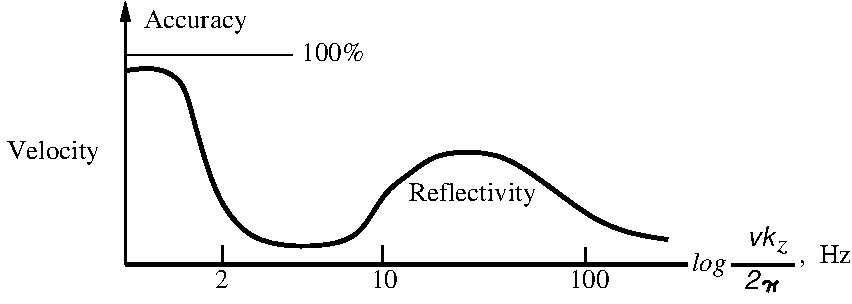
\includegraphics[width=0.5\textwidth]{xrf/rely}
\caption[rely]{根据地面地震观测所得信息之可靠性程度}
\label{fig:xrf/rely}
\end{figure}
注意,从2赫兹至10赫兹,存在有一个信息空白段。即使假设岩石物理学可以给我们提供密度$\rho$与
不可压缩性系数$K$之间的关系,这个空白也会严重妨碍地震学家在进行钻井之前就能预测测井记录情况
的能力,地震学家能够作得可靠一点的只是对已经过滤波处理的测井记录进行预测而已。

上述观测情况使得反射地震学家不得不把“速度”这个词当作一个专用术语来用了。对
反射地震学家来说,速度的意思就是指“真速度”的低空间频率部分,“真速度”的高频部分
从未称作速度,而是称作反射率(reflectivity)。密度由于几乎无法根据地面反射地震学
来测定,通常都不注意它。

\subsection{数学反演问题}
在数学中,求解一个反演问题的意思就是根据波场来“决定”介质性质,往往是采用一
个“收敛序列”来达到这个目的。而地球物理学所指的“决定”究竟是什么意思却不太严谨
(或者包括内容太多)。在本书的第一章至第二章中,反射面是根据自激自收概念“决定”
的;在第三章中,又同炮检距结合起来了,反射率与速度则以观测排列延拓的概念
来“决定”;在第五章中,这种概念发展为抑制多次反射然后再令下行波初动时间以前出现
的上行波等于零的办法来求取反射的“真”振幅。看来很可能未来的处理方法还要形成一些
其他成像概念,也许有可能证明我们的某些“决定”同数学家的那些“决定”是符合一致
的,但是这样的符合一致并不是我们的目标。

\subsection{声波波动方程的导出}
声波波动方程描述液体内或气体内的声波,另一种更复杂的方程组描述固体中的弹性
波。现在从声波情形开始讨论。牛顿动量守恒定律说,气体之内的一个小体积将因有力的作
用而加速,力由小体积的相向两端上的压力差所形成。现定义\\
$\rho$=流体每单位体积的质量;\\
$u=x$方向的流体流动速度;\\
$\omega=z$方向的流体流动速度;\\
$P=$流体内之压力;\\
牛顿定律说:\\
质量$\times$加速度=力=$-$压力梯度\\
\begin{subequations}\label{eq:ex1.4.3}
\begin{equation}
\rho\frac{\partial u}{\partial t}=-\frac{\partial P}{\partial x} \label{eq:ex1.4.3a}
\end{equation}
\begin{equation}
\rho\frac{\partial\omega}{\partial t}=-\frac{\partial P}{\partial z} \label{eq:ex1.4.3b}
\end{equation}
\end{subequations}
因压缩与体积变化而形成能量储集是第二种物理过程。如在$x+\Delta x$点上的速度向量
$u$超过在$x$点上的速度,则说流动是发散的。换言之,$x$与$x+\Delta x$之间的小
体积正在膨胀。这种膨胀必然导致有一压力降,压力降的大小与称作不可压缩性系数尺的
流体性质成比例,在一维情形下,该方程为\\
压力降=不可压缩性系数$\times$速度之散度\\
\begin{subequations}\label{eq:ex1.4.4}
\begin{equation}
-\frac{\partial P}{\partial t}=K\frac{\partial u}{\partial x} \label{eq:ex1.4.4a}
\end{equation}
在二维情形下则为
\begin{equation}
-\frac{\partial P}{\partial t}=K(\frac{\partial u}{\partial x}+\frac{\partial \omega}{\partial z}) \label{eq:ex1.4.4b}
\end{equation}
\end{subequations}
为从式\ref{eq:ex1.4.3a}与\ref{eq:ex1.4.4a}得出一维波动方程,首先用$\rho$除式\ref{eq:ex1.4.3a}并对$x$求导
\begin{equation}
\frac{\partial }{\partial x}\frac{\partial}{\partial t}u=-\frac{\partial}{\partial x}
\frac{1}{\rho}\frac{\partial P}{\partial x}
\label{eq:ex1.4.5}
\end{equation}
其次,对式\ref{eq:ex1.4.4}取时间导数。在固体地球科学中,我们很幸运的是问题中的
物质在我们进行试验期间并不改变,这意味着$K$不是时间$t$的函数
\begin{equation}
\frac{\partial^2 P}{\partial t^2}=-K\frac{\partial }{\partial x}\frac{\partial}{\partial t}u
\label{eq:ex1.4.6}
\end{equation}
将式\ref{eq:ex1.4.5}代入式\ref{eq:ex1.4.6},得一维标量波动方程
\begin{subequations}\label{eq:ex1.4.7}
\begin{equation}
\frac{\partial^2 P}{\partial t^2}=-K\frac{\partial }{\partial x}
\frac{1}{\rho}\frac{\partial P}{\partial x} \label{eq:ex1.4.7a}
\end{equation}
在二维空间内,准确的声学标量波动方程为
\begin{equation}
\frac{\partial^2 P}{\partial t^2}=K(\frac{\partial }{\partial x}
\frac{1}{\rho}\frac{\partial P}{\partial x}+\frac{\partial }{\partial z}
\frac{1}{\rho}\frac{\partial P}{\partial z} )\label{eq:ex1.4.7b}
\end{equation}
\end{subequations}
你经常会见到简化形式的标量波动方程,在这种形式的方程中,假设$\rho$不是$x$与$z$的函数,采
用这种近似一般有两个理由:一是因观测结果一般都不能确定密度,所以最好是把密度取为
常数;二是如果该系数是空间变量的函数,傅氏变换方法求解就无法适用了。在考察这种近
似是否成立之前,先考察一下由此会得何种结果。采取这种近似,直接就可将式\ref{eq:ex1.4.7b}
简化成标量波动方程的通常形式
\begin{equation}
\frac{\partial^2 P}{\partial t^2}=\frac{K}{\rho}(\frac{\partial^2}{\partial x^2}+
\frac{\partial^2}{\partial z^2})P
\label{eq:ex1.4.8}
\end{equation}
代入试验解
\begin{equation}
P=\exp (-i\omega t+ik_xx+ik_zz)
\label{eq:ex1.4.9}
\end{equation}
就可看出这个方程不过是重述前数节中的儿何概念,所得就是二维波动方程的波散关系
\begin{equation}
\frac{\omega^2}{K/\rho}=k_x^2+k_z^2
\label{eq:ex1.4.10}
\end{equation}
早先(1.2节式\ref{eq:ex1.2.8}),只考虑波的几何性态就建立过类似于式\ref{eq:ex1.4.10}的方程。在那
种处理办法中,已经发现式\ref{eq:ex1.4.10}
中的$K/\rho$就是波速的平方根。物理学与几何学就这样
经由下列联系而和谐一致了
\begin{equation}
v^2=\frac{K}{\rho}
\label{eq:ex1.4.11}
\end{equation}
最后,让我们看一下为什么在速度是空间可变时就不能采用傅氏变换方法。设$\omega$、$k_x$与$k_z$均是
非空间坐标的函数,将\ref{eq:ex1.4.9}式代入\ref{eq:ex1.4.8}式内,于是你就得到矛盾结果;如
果速度是空间坐标的函数,那么$\omega$、$k_x$与$k_z$就都必须是空间可变的。再假设它们全具有空间
可变性,于是所得方程将仍然是一种偏微分方程,而不是像式\ref{eq:ex1.4.10}那样的一种代数方程。

\subsection{倏逝波与地滚波}
完成波散关系的物理推导,得
\begin{equation}
k_x^2+k_z^2=\frac{\omega^2}{v^2}
\label{eq:ex1.4.12}
\end{equation}
我们现在可以对它有一种新考虑,它带来了远比早先根据几何推导所能设想到的更为多的意
义。原先只不过把波散关系看成是体现一种几何关系$cos^2\theta+sin^2\theta=1$,其中
所以$sin\theta$超过1是没有意义的,换言之,$vk_x$超过$\omega$是没有意义的。现在在这里却是有意义
的,前面述及两种偏移方法中都隐藏了一个未加解释说明之赴,既然数据资料可以是$(t,x)$
平面中的一个任意函数,那么它的傅氏变换当然就可以是$(\omega,k_x)$平面内的一个任意
函数了,于是,实际上总是存在有角度的正弦会大于1的能量,这种情形如图\ref{fig:omk/evtheory}所示。应
该怎么对待这种能量呢?
\begin{figure}[H]
\centering
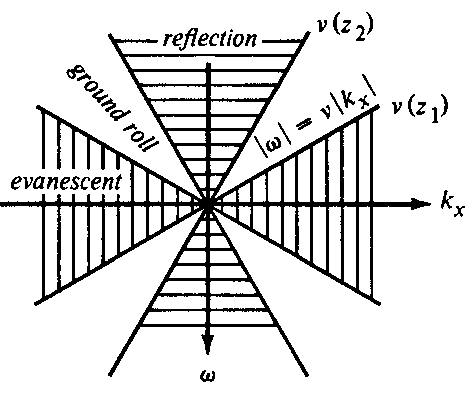
\includegraphics[width=0.5\textwidth]{omk/evtheory}
\caption[evtheory]{反射能量的三角形区域$|\omega|>v(z)|k_x|$随速度$v$的增大,因而
也就是随深度$z$的增大而变得更窄。地滚波是沿地面传播的能量,而指数衰减波则是地下深处传播的
能量}
\label{fig:omk/evtheory}
\end{figure}

$vk_x$在超过$\omega$时,最好将熟悉的向下外推算子改写成
\begin{equation}
e^{\pm i\sqrt{\omega^2/v^2-k_x^2}}\cdot x=e^{\pm\sqrt{k_x^2-\omega^2/v^2}}\cdot x
\label{eq:ex1.4.13}
\end{equation}

这个式子说明,物理解的深度依从关系是一种增长指数形式或一种阻尼指数形式,这些解称
作倏逝波\footnote{原文为evanescence,直译应为“消散波”或“耗散波”,“倏逝波”这种波具有按指数规律迅速变化的性质,而且有意义的是按负指数规律变化的波。——译者}(evanescent wave)。在最极端情形$\omega=0$时,$k_x$是实数,从而$k_x=\pm ik_x$。
对于弹性波,这点可用地面在一架停泊飞机的作用下所发生的形变来举例说明。仅当飞机运动速度高
于波在地层内之传播速度时,才会有一个波辐射进入地下。如飞机以亚音速运动,这时发生
的形变叫作准静态形变。

以具有正弦形皱纹的薄板进行假想试验,也许是一
种比较好的物理描述方法。这样的金属薄板有时用作房
顶或汽车库大门。皱纹之波长固定了$k_x$值。这样的薄板
以速度$V$运动经过你耳朵时,不论$V$是否大于还是小于
空气中的声速,你都会听到一种振荡频率等于$Vk_x$的声
音,但是你听到的声音将随离开该薄板之距离而指数衰
减,除非它运动得非常之快$(V>v)$。在这种情形下,
运动着的薄板辐射出的声音会达到很远距离。这就是超
音速飞机为什么使用如此大量燃料的原因。

偏移程序对运动速度低于声速的能量应该有什么影
响呢?理论上,这种能量应当沿着离开震源远去的方向
作指数衰减,在$(\omega,k_x)$空间抑制带区域内的阻尼衰
减极快速。因而,简单的爆炸反射面理论预言,在速度
低时,资料内应该几乎就不存在能量。

但是真实情形是:$(\omega,k_x)$空间的指数衰减区域内不是有极少量能量,而总是存在大
量能量,爆炸反射面概念又一次破产了。处理陆地地震资料时,问题更糟糕。在深处速度
较快的岩石内作指数衰减的波可以在低速土壤层中传播,这种能量称作迆滚波,图\ref{fig:omk/evdata}
是一个例子。像起伏变化很大的地表面一样,控制着地滚波的最浅地下界面也是变动很大
的,所以虽然图\ref{fig:omk/evdata}是一个好例子,但没有一个例子可以真正是典型的。
这个资料不是零炮检距剖面,炮点在左侧,而右侧各记录道则由离炮点距离逐渐増大的裣波器所产生。图上
绘有直线,其斜率相应于海水层的速度,较陡的同相轴全是地滚波。在这张图中,存在两类
地滚波。有一类其速度大约等于海水层速度的一半;振幅较强的一类其速度大约等于海水层
速度的四分之一,该种到达较迟而振幅较强的一类地滚波具有以频散现象而知名的有趣恃
征,从上下关系来观察该资料,你应能注意到高频到达早于低频。
\begin{figure}[H]
\centering
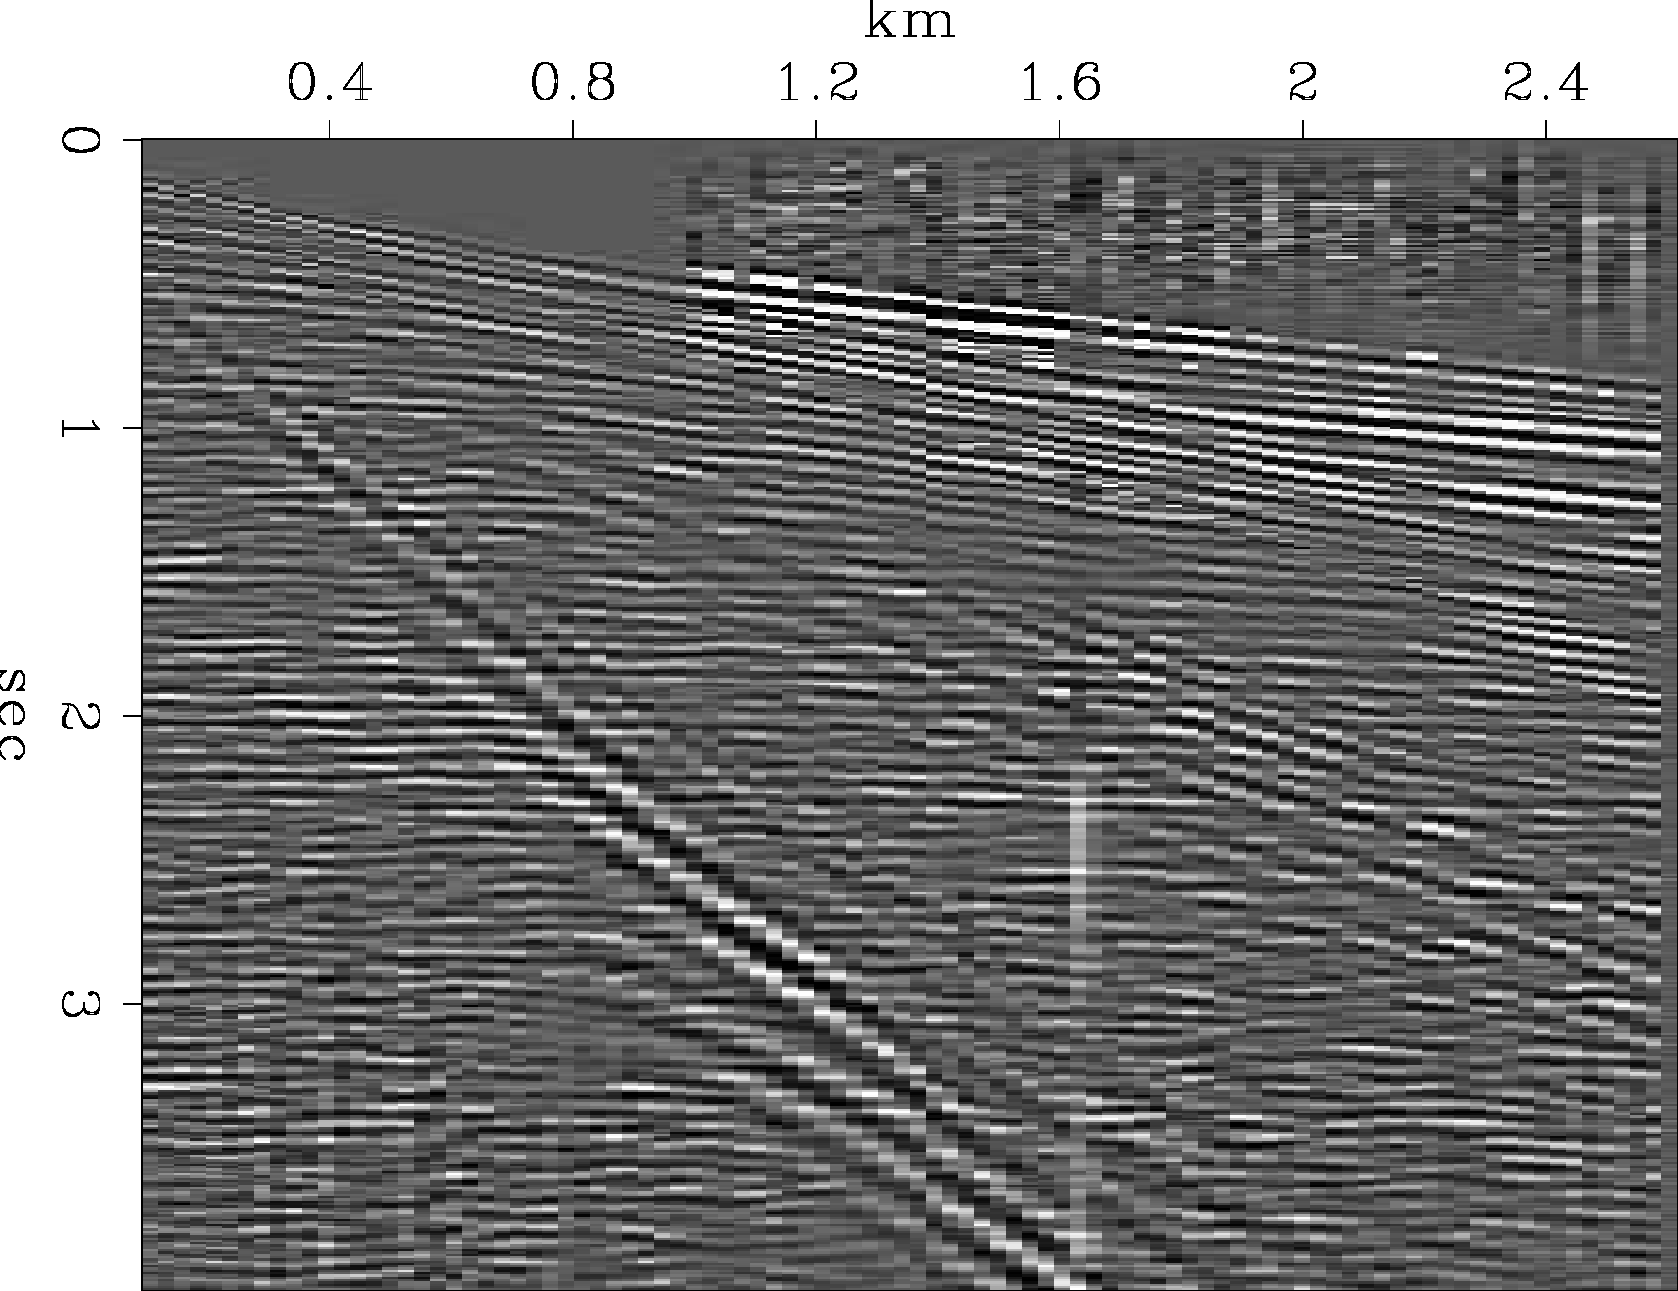
\includegraphics[width=0.5\textwidth]{omk/evdata}
\caption[evdata]{佛罗里达浅海地震剖面,显示具有频散现象的地滚波}
\label{fig:omk/evdata}
\end{figure}
由于地滚波指数衰减有效地防止了它受深层目的层的影响,所以地滚波成了不受欢迎的
干扰。在实际处理中,应使$(\omega,k_x)$空间抑制带区域内的能量衰减掉,用数学语言描述就是
说,从模型空间至数据空间、然后又返回模型空间的这种合成映像过程,不是一种恒等变换
而是一种等幂变换。
\subsection{反射与高频极限}
众所周知,两种不同物质的接触面可以引起反射。不可压缩性系数AT或密度P以空间阶
跃函数形式改变的地方,就定义为物质接触面。在一维情形下,$\frac{\partial K}{\partial x}$、$\frac{\partial\rho}{\partial x}$或者二者会在某
一点上成为无限大,并且我们知道,任一种都可以形成反射。所以,也许有点奇怪,密度的
导数是明显出现在式\ref{eq:ex1.4.7b}内,而不可压缩性系数的导数却未明显在该式中出现,
这意昧着略去式\ref{eq:ex1.4.7b}中的密度梯度,并不会消去所有可能的反射。可是,略去该项会使进
一步的分析稍微简化,而且因为恒定密度是一种合理的情形,所以总是略掉该项的。

还存在有一些众所周知的数学条件,在该条件下,一阶项均可略去。现在集中注意一个
沿任何特定方向传播的波,这时,$\omega$,$k_x$和$k_z$都有某种规定的值。
在频率趋向无限大的极限情形时,式\ref{eq:ex1.4.8}内的诸二阶导数项$P_{11}$、$P_{xx}$与$P_{xx}$
均趋于无限大的二次幂。假设两种介质逐渐彼此混合,从而使密度梯度小于无限大,于是式\ref{eq:ex1.4.7b}导出式\ref{eq:ex1.4.8}时出现的形式为$\rho_xP_x$与$\rho_xP_x$的一阶导数乘积项,均可忽略不计,因为这些项在频率趋向无限大时仅趋于无限大的一次幂,因而可在该种极限情形下将其忽略不计。

目的在于计算合成地震记录的理论地震学中,通常要包括这些项,但在目的在于根据地
震野外数据作出地层模型的场合——如本书中的场合——一般是忽略这些项的。地层成像
比计算合成地震记录要困难得多,忽略这些项的理由往往只不过是为了减少麻烦;为将方程写
成二维而不是三维形式(推广至三维通常是可能的,但往往并不要求如此),根据同样的理
由也能忽略这些项。此外,总是要忽略这些项以便于采用傅氏变换方法。也许会出现需要这
些项使之包括在内的实际情况,如果是这样,采用有限差分方法(见2.2节)不难将它们包
括在内。但是任何企图将它们包括在数据处理之中的努力,也应当注意考虑具有类似意义的
其它因素,诸如要假设声波方程可以近似应用于弹性介质情形等等。

\subsection{习题}
\begin{enumerate}
\item 在一定深度的潜水面之下,土壤为水所饱和是典型情形。采用重锤地震仪记录系
统的工作经验证明,地震波速度的典型情形是在潜水面上突然跃变为水的速度($V_{water}=
m/s$)。据说,在一定位置上观察到地滚波要比反射波强一些,所以决定把检波器埋置在地
面下。观测到这种引起麻烦的地滚波的传播速度等于水的速度的十分之六。要使地滚波衰减
十倍,试问检波器必须埋置潜水面之下多深?假设所帶数据资料已包含从10赫兹至100赫兹
的所有频率。(提本:$log_e^{10}\approx 2$,$2\pi\approx 6$等等)
\item 设有一维波动方程
\begin{equation}
(\frac{\partial^2}{\partial t^2}-\frac{K(z)}{\rho(z)}\frac{\partial^2}{\partial z^2})P=
-\frac{K(z)}{\rho(z)^2}\frac{\partial \rho}{\partial z}
\frac{\partial P}{\partial z}
\label{eq:ex1.4E1}
\end{equation}
现考虑以下列函数作为试验解
\begin{equation}
P(z,t)=P_0\frac{1}{\sqrt{Y(z)}}\exp(i\omega t-i\int_0^x\omega\sqrt{\frac{\rho(\xi))}{K(\xi)}}d\xi)
\label{eq:ex1.4E2}
\end{equation}
式中\\
$P_0=const.$\\
$Y\equiv\frac{1}{\sqrt{\rho(z)K(z)}}$\\
将试验解\ref{eq:ex1.4E2}代入波动方程\ref{eq:ex1.4E1},试讨论在物性参量允许变化与不同波长情形下的解
均能成立这两种要求之间应如何权衡折衷。
\end{enumerate}




\section{旁轴波动方程}
标量波动方程不像傅里叶(Fourier)方程,是允许密度与速度有任意的空间变动的。
你也许因为这一点而期望能把它直接用于偏移剖面的生产,但其实它很少用于偏移,因而我
们将首先回顾一下为什么会这样,然后我们将会讨论旁轴波动方程(paraxial wave equation),
它是大多数生产性偏移处理的基础。

就基本原理而言,旁轴波动方程可以说是射线和平面波这类简单概念与波动方稈湿体现
深刻概念之间的一釉折衷产物。旁轴波动方程也称作单平方根方程(Single-square-root
equation),在第二章中,它有一个专用名词,称作抛物线波动方程(parabolic wave
equation)导出抛物线波动方程不是从古典物理的简单概念着手的,它的建立就像量子物理
学中的薛丁格方程(Schroedinger equation)那样,颇为转弯抹角,
你必须下点功夫研究,才看得出为什么需要如此。当我在1970年把抛物线波动方程引进到
地震计算中去时,曾经遇到相当多的怀疑。你很幸运,多年的经验已经使我能比较好地完成
解释它的任务了。对我来说,也很幸运,这种方法在工业应用舞台上占有优势地位将会引起
你坚持学下去的兴趣。

旁轴波动方程将藉助于傅氏变换方法导出。傅氏变换方法同空间可变系数是不相容的,
由于我们想使速度体现出空间变化,需要最大限度地避免这种限制性,所以在傅氏变换域内
得到旁轴方程之后,就将$ik_x$用$\partial /\partial x$代替,将认$ik_z$用
$\partial /\partial z$代替。由于现在是在空间域内了,速度
也可以是空间可变的了。所得结果是一种恒可用有限差分方法求解的偏微分方程。这种处理
办法已证明是成立的,但是学习偏移方法的新学生对这种处理还有疑虑,这是可以理解的。
考虑到这点,本节最后部分将讨论一种不采用傅氏变换方法而导出旁轴波动方程的办法。

\subsection{为何标量波动方程很少用于偏移}
要是偏移真能用标量波动方程处理而不是用旁轴方程,那事情就能简单一些了。确实,
偏移是可以甩标量波动方程处理,而且还有若干潜在的好处(Kosloff与Baysal,1983)。
但是,99\%以上的现行工业性偏移应用却是藉助旁轴方程完成的。

采用标量波动方程时的主要问题在于它会产生不希望有的层内多次反射,但是爆炸反射
面概念却是不能处理多次波的。一次反射只能用上行波模拟,而多次反射既涉及上行路程又涉
及下行路程,实际工作中观察到的多次反射完全不同于爆炸反射面概念预言的结杲。对海底
多次反射来说,双程旅行时间深度为$t_0$的海底在$2t_0$、$3t_0$、$4t_0\ldots\ldots$等时刻形成海底多次反
射;在基于爆炸反射面概念的模型中,单程旅行时间深度为的海底是在$3t_0$、$5t_0$、$7t_0\ldots\ldots$
等时刻形成海底多次反射。在制造望远镜、显微镜或摄影机时,设计者很注意要压制向后反
射的光,因为它在影像上形成背景干扰。与此类似,在建立一个偏移程序时,我们不希望有
对聚焦成像毫无作用的能量在周围移动。带有空间可变系数的标量波动方程就会产生此类能
量,如果它是相干能量而且偏移至一次波较弱的某个时间上,这种不受欢迎的能量就特别麻
烦。它之使人烦恼讨厌,正如在电视屏幕上能见到明亮窗户的反射影子一样令人烦恼。所
以,你如果要试图用标量波动方程来进行偏移,你就得使速度尽可能地平滑。

采用标量波动方程进行成像时的另一种困难是由于倏逝波所形成的,这些波是随深度而
指数增长或衰变的波。大自然是沿正向时间将波外推,而我们则将它们向深度方向外推。增
长指数有微不足道的扰动、甚至数值上是可舍入的零头,就能产生很大影响。因为它增长速
度快,所以必须找到某些手段来压制它们。

采用标量波动方程进行成像时的第三个困难源出于初始条悴。标量波动方程有一项深
度$z$的二阶导数,这意味着要求在$z$轴上有两个边界条件。因为数据是在$z=0$时记录的,看来
很自然,这些边界条件就应该是$z=0$时的波场$P$和波场梯度$\partial P/\partial z$、,可是$\partial P/\partial z$如并没有在地面上记录。

幸好,建立某神整个是在计算机内部运算的成像方法时,我们有理想的工具可资利用,
这就是无反射透镜。或者说,我们不是用现实世界的标量波动方程而是用旁轴波动方程。

\subsection{旁轴波动方程的Fourier导出方法}
现在从标量波动方程的波散关系开始
\begin{equation}
k_x^2+k_z^2=\frac{\omega^2}{v^2}
\label{eq:ex1.5.1}
\end{equation}
取平方根
\begin{equation}
k_z=\pm\sqrt{\frac{\omega^2}{v^2}-k_x^2}
\label{eq:ex1.5.2}
\end{equation}
在式\ref{eq:ex1.5.2}内选择负号,意味着是取上行波而消去下行波。式\ref{eq:ex1.5.1}是标量波动方程\\
$\frac{\partial^2 P}{\partial x^2}+\frac{\partial^2 P}{\partial z^2}=\frac{1}{v}\frac{\partial^2 P}{\partial t^2}$\\
的三维傅氏变换结果,对式\ref{eq:ex1.5.2}进行反变换则将给出一个仅为上行波(或下行波)而
无其他波的方程。对某个坐标轴的逆傅氏变换只不过是选择下列一种代换的问题
\begin{subequations}\label{eq:ex1.5.3}
\begin{equation}
\frac{\partial}{\partial t}=-i\omega
\end{equation}
\begin{equation}
\frac{\partial}{\partial x}=ik_x
\end{equation}
\begin{equation}
\frac{\partial}{\partial z}=ik_z
\end{equation}
\end{subequations}
对$z$轴进行逆变换之后,就得一个关于$z$的偏微分友程。速度在该方程中可以取$z$为变量,对
$x$轴也可得类似结果。式\ref{eq:ex1.5.3}中任何一种代换代入式\ref{eq:ex1.5.2}而得出的任何一种结果,就
称为旁轴方程,本书第二章将详细讨论这些方程的意义。在开始这样解释旁轴波动方程之前,
要讨论一下不采用傅氏变换如何导出它。除了获得导致基本偏移方程的清晰思路之外,这种
导出方法还能使我们更好地理解该方程真正能作什么,以及它如何不同于标量波动方程。
\subsection{斯涅尔(Snell)波}
研究波扬很自然要从描述恒速介质内的平面波的方程开始。不过,在反射地震勘探中,
最浅与最深反射面之间的速度差异一般都超过两倍,为此,在分析野外资料时差不多总得包括
速度随深度的变化。除了要迁就适应分层速度$v(z)$)以外,地震学理论需要考虑的正是像乎
面波那样的波。图\ref{fig:omk/airplane}所示就是这样一种理想情形:水平飞行的超音速飞机辐射出的波传
播进入地下。
\begin{figure}[H]
\centering
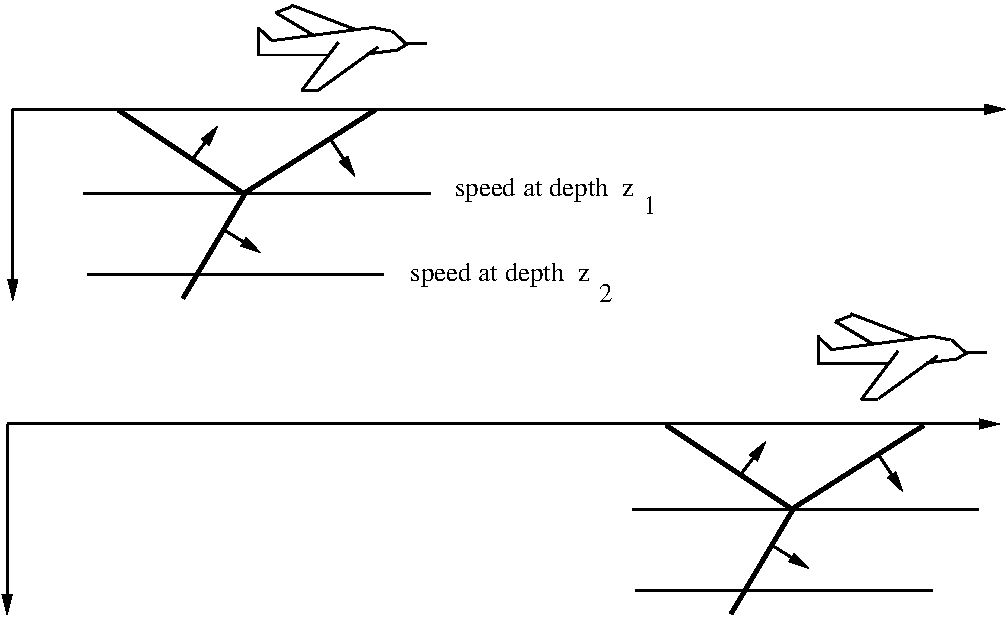
\includegraphics[width=0.5\textwidth]{omk/airplane}
\caption[airplane]{疾翔的飞机辐射出声波进入地中。由图你可得出结论:在深度为$z_1$之处和深度为$z_2$之处的
$\partial t/\partial x$是相同的;在各向同性介质中,这个结论就导出Snell定律}
\label{fig:omk/airplane}
\end{figure}
飞机以恒速水平飞行,从$x=-\infty$飞至$x=+\infty$。试想像有一水平平面成层地层,在这种模
型中,尤轴上的任何点同$x$轴上任何其他点之间毫无区别,但是地震波速度是逐层变化。可能
存在反射、折射、横波及多次反射。不管图形如何,它是随飞机而一起运动的,于是可想像
飞机附近的波阵面图像也随飞机而一起运动。即使地层速度是随深度而增大的,该图的顶部
与图的底部也都是以相同速度沿
水平方向运动,如果顶部与底部不是相同速度,图形就会畸变,
同所假设的平移对称性相矛盾。这种水平速度,或更确切地说,这
种速度的倒数$\partial t/\partial x$,有若干个名称,在实际工作中,将它称作时
差。在理论工作中,则称它为射线参量。注意到这点是非常重要
的:$\partial t/\partial x$不随深度而变化,即便地震波速度是随深度而变化
的。在恒速介质中,波传播方向的角度不随深度而变化,在成层
介质中,$\partial t/\partial x$不随深度而变化。

波的微分几何关系如图\ref{fig:omk/frontz}所示。该图表明
\begin{subequations}\label{eq:ex1.5.4}
\begin{equation}
\frac{\partial t}{\partial x}=\frac{sin\theta}{v}
\label{eq:ex1.5.4a}
\end{equation}
\begin{equation}
\frac{\partial t}{\partial z}=\frac{cos\theta}{v}
\label{eq:ex1.5.4b}
\end{equation}
\end{subequations}

这两个方程定义两个速度(速度倒数)。第一个是沿地表面测定的
水乎速度,称为水平相速度;第二个是沿钻孔深度方向测定的垂
直速度,称为垂直相速度。注意,这些速度全都大于波在介质
中的传播速度$v$。由波阵面在坐标轴上的投影得出的速度都大于
$v$,而由射线在坐标轴上的投影得出的速度都小于$v$。相速度的倒数称为时差(stepout
)或者慢度(slowness)。
\begin{figure}[H]
\centering
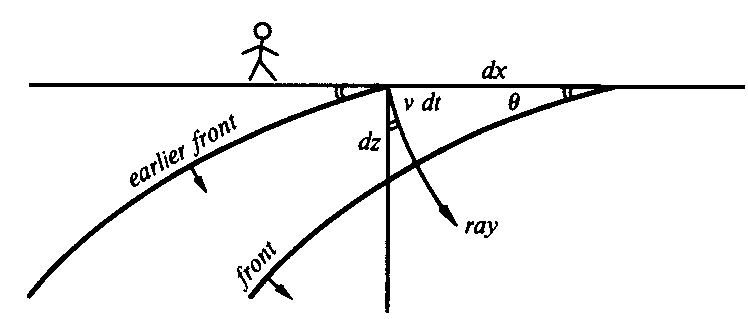
\includegraphics[width=0.5\textwidth]{omk/frontz}
\caption[frontz]{成层介质$v(z)$中的下行波阵面与射线,波阵面彼此平行平移}
\label{fig:omk/frontz}
\end{figure}

斯涅尔定律将波在一层内的传播角度同在另一层内的传播角度联系在一起。式\ref{eq:ex1.5.4a}
沿深度方向应恒定不变,实际上正是斯涅尔定理的证明。确实,我们已经导出的正是斯涅尔
卑律在地震学中,所有的波均在速度分层介质中传播,所以不能把它们称为平面波。但是
我们需要对接近于平面波的那些波取个名宇,将平面波概念推广至成层介质$v(z)$的情形,把它
定义为斯涅尔波。一个平面波恰好进入速度$v(z)$随深度而变的某种介质,就变成了一个斯涅
尔波,当平面波具有某种传播方向角度时,就用一个斯涅尔参量$p=\partial t/\partial x$来代替斯涅尔波。

值得注意的是,斯涅尔参量$p=\partial t/\partial x$加可在地面上直接观测,而$v$与$\theta$却没一个能直接观
测。因为$p=\partial t/\partial x$不但可观测,而且沿深度方向恒定不变,所以习惯上都利用这点从式\ref{eq:ex1.5.4a}
中消去$\theta$
\begin{subequations}\label{eq:ex1.5.5}
\begin{equation}
\frac{\partial t}{\partial x}=\frac{sin\theta}{v}=p
\label{eq:ex1.5.5a}
\end{equation}
\begin{equation}
\frac{\partial t}{\partial z}=\frac{cos\theta}{v}=[\frac{1}{(v(z))^2}-p^2]^{1/2}
\label{eq:ex1.5.5b}
\end{equation}
\end{subequations}
令斯涅尔波通过零时间的原点,则任何其他位置上的斯涅尔波到达时间表达式由下式给
出
\begin{subequations}\label{eq:ex1.5.6}
\begin{equation}
t(x,z)=\frac{sin\theta}{v}x+\int_0^x\frac{cos\theta}{v}dz
\label{eq:ex1.5.6a}
\end{equation}
\begin{equation}
t(x,z)=px+\int_0^x[\frac{1}{(v(z))^2}-p^2]^{1/2}dz
\label{eq:ex1.5.6b}
\end{equation}
\end{subequations}
计算出$\partial t/\partial x$与$\partial t/\partial z$,然后与式\ref{eq:ex1.5.5}比较,很容易检查证明式
\ref{eq:ex1.5.6b}成立。

斯涅尔波可具有任意波形$f(t)$,利用式\ref{eq:ex1.5.6}定义一个延迟时间$t_0$,则位于$(x,z)$
位置上的延迟波$f[t-t_0(x,z)]$将为
\begin{equation}
SnellWave(t,x,z)=f[t-px-\int_0^x[\frac{1}{(v(z))^2}-p^2]^{1/2}dz]
\label{eq:ex1.5.7}
\end{equation}
\subsection{时移方程}
在已知地面上的波形条件下,预测地层内部的波场,是一项重要任务。对于下行平面
波,可用下列时移偏微分方程实现这点
\begin{equation}
\frac{\partial P}{\partial z}=-\frac{1}{v}\frac{\partial P}{\partial t}
\label{eq:ex1.5.8}
\end{equation}
将试验解
\begin{equation}
P=f(t-\frac{z}{v})  \quad\quad\quad for\quad constant\quad v
\label{eq:ex1.5.9}
\end{equation}
或
\begin{equation}
P=f(t-\int_0^z\frac{dz}{v(z)})  \quad for\quad v(z)
\label{eq:ex1.5.10}
\end{equation}
代入很容易就能证明确实如此。

对于非垂直入射情形,下述偏微分方程也能成立
\begin{equation}
\frac{\partial P}{\partial z}=-\frac{\partial t}{\partial z}\frac{\partial P}{\partial t}
\label{eq:ex1.5.11}
\end{equation}
该方程的解为
\begin{equation}
P=f(t-px-\int_0^z\frac{\partial t}{\partial z}dz) 
\label{eq:ex1.5.12}
\end{equation}
解释式\ref{eq:ex1.5.11}与\ref{eq:ex1.5.12}时,要记住$1/(\partial t/\partial z)$是垂向视速度。波场$P$关于深度$z$的偏
导数是在恒定$x$时取的,即向下外推波场。只用时移就可达到向下外推效果的这种思想,仅
当存在一个斯涅尔波时才成立,就是说,在所有位置上看见的必须是同一个任意时间函数。

将式\ref{eq:ex1.5.5}代入时,还能使我们把式\ref{eq:ex1.5.11}改写成各种不同的形式
\begin{subequations}\label{eq:ex1.5.13}
\begin{equation}
\frac{\partial P}{\partial z}=-\frac{cos\theta}{v}\frac{\partial P}{\partial t}
\label{eq:ex1.5.13a}
\end{equation}
\begin{equation}
\frac{\partial P}{\partial z}=-[\frac{1}{(v(z))^2}-P^2]^{1/2}\frac{\partial P}{\partial t}
\label{eq:ex1.5.13b}
\end{equation}
\begin{equation}
\frac{\partial P}{\partial z}=-[\frac{1}{(v(z))^2}-(\frac{\partial t}{\partial x})^2]^{1/2}\frac{\partial P}{\partial t}
\label{eq:ex1.5.13c}
\end{equation}
\end{subequations}
式\ref{eq:ex1.5.13}是一个旁轴波动方程。由于$\partial t/\partial x=p$可沿地表面测定,看来将方程\ref{eq:ex1.5.13c}同某 种观测数据$P(t,x,z=0)$和假设的一种速度$v(z)$结合一起,将使我们有可能确定。这是
向下延拓的必要的第一步,不过必须假设仅存在一个斯涅尔波而不是若干斯涅尔波的叠加才
行。不同斯涅尔路程上的不同波形叠加起来,就会造成在不同位置上看到不同时间函数的结
果。于是,仅一次时移将达不到向下延拓的目的。幸好,一个逐点可变的复杂波场能够分解
成许多斯涅尔波,其中每一个均可用微分方程\ref{eq:ex1.5.13}或者它的解\ref{eq:ex1.5.12}来实现向下
延拓,这样一种分解方法就是傅里叶分析。 

\subsection{傅氏分解}
对地表面上看到的函数$f(x,t,z = 0)$进行傅里叶分析时,要求傅氏积分核为$exp(-i\omega t+ik_xx)$。以速度倒数
$\partial t/\partial x=k_x/\omega$沿地表面运动时,傅氏积分核的相位应保持为常数,因而
也就是积分核本身保持为常数。这时,只有以与斯涅尔波相同的速度运动的那些正弦分量,
才可以使该斯涅尔波具有非零的相关关系。因此,如果扰动是一个斯涅尔波,则除了满足
$p=k_x/\omega$关系的那些分量之外,所有傅氏分量均为零。你应当记住这些基本关系
\begin{equation}
\frac{\partial t}{\partial x}=\frac{sin\theta}{v}=p=\frac{k_x}{\omega}
\label{eq:ex1.5.14}
\end{equation}
在理论地震学中,由于利用式\ref{eq:ex1.5.14}求取一个余弦,结果总是出现平方根函数。

利用斯涅尔参量户的这种傅氏变换域解释,能使我们把平方根方程\ref{eq:ex1.5.13}写成更为
有用的形式。但是首先必须在傅氏变换域内表达平方根方程,将\ref{eq:ex1.5.13}中的算子$\partial /\partial t$用
$-i\omega$代替,就可完成这点,结果为
\begin{equation}
\frac{\partial P}{\partial z}=+i\omega[\frac{1}{(v(z))^2}-\frac{k_x^2}{\omega^2}]^{1/2}P(\omega,k_x,z)
\label{eq:ex1.5.15}
\end{equation}
现在,它等价于把微分方程\ref{eq:ex1.5.15}
或者它的解\ref{eq:ex1.5.12}具体化为如下复指数,
\begin{equation}
P(\omega,k_x,z)e=exp\{i\omega\int_0^z(\frac{1}{(v(z))^2}-\frac{k_x^2}{\omega^2})^{1/2}dz\}
\label{eq:ex1.5.16}
\end{equation}
以后,当我们考虑可横向变化的速度$v(x)$时,这个解\ref{eq:ex1.5.16}就变成错误的了,然而微分方程\ref{eq:ex1.5.13c}描述任何局部平面波性态却仍旧有效。但是,在准备处理横向速度梯度问题
以前,我们应当更仔细地研究一下垂直速度梯度。

\subsection{速度梯度}
将斯涅尔波场表达式代入标量波动方程中时,我们发现,我们的斯涅尔波的定义并不满
足该标量波动方程。不过,这种偏差仅发生在出现有速度梯度时。换言之,如果浅层恒定速度
为$v_1$,深层恒定速度为$v_2$,则除了在$v_1$变为$v_2$之处外,方程处处可被满足。因透过系数之
故,经过分界面时,标量波动方程的解必然表现有振幅变化,我们所定义的斯涅尔波则是一
种随深度之变化而只有恒定振幅的波。旁轴波动方程可加以修正,使之能反映透过系数的影
响。现在所以很少进行这种修正,其原因可能同恒可忽略密度梯度的原因相同,在它们可改
善所得结果、即给出更正确的振幅与可能的微小相移的同时,它们也使方程增加了杂乱干扰
的影响,抵销了所得好处。说实在的,如果要求这样作,那么就应当回答其他更深刻的问
题,诸如为什么不是利用标量弹性方程的各种不同其他形式而是利用声学方程。

即使修正旁轴波动方程使之能同透过系数影响结合起来,但由于缺乏反射波,它的解将
仍然无法满足标量波动方程。但是那好极了,因为正是具有无反射透镜作用的旁轴方程才是
数据处理所期望的方程。

\subsection{习 题}
\begin{enumerate}
\item 试设计一种平面波数学表达式,要求它是时间的脉冲函数,传播方向与垂直轴2正
方向所夹角度为15°。试在下列域内表示所得结果
\begin{table}[!ht]
\centering
\ttfamily
\small
%\begin{tabularx}{\textwidth}{Y|Y}
\begin{tabular}{p{3cm}p{4cm}}
\toprule
\midrule
 (a)& $(t,x,z)$\\
 (b)&$(\omega,x,z)$ \\
 (c)&$(\omega,k_x,z)$\\
 (d)&$(\omega,p,z)$ 
%\bottomrule
%\end{tabularx}
\end{tabular}
\end{table}
\item 试求振幅函数$A(z)$,当乘以式\ref{eq:ex1.5.12}中的函数$f$时,可成为分层介质$v(z)$的
标量波动方程近似解。对于$p=0$的情形,该解应化简为1.4节中习题(2)的解。
\end{enumerate}


\section{二维傅氏变换技巧}
\label{sec:1.6}

本节内容是对那些将要从事偏移方法处理的人们有用的提示大全。

\subsection{傅氏变换中的符号与比例因子}
\label{sec:1.6.1}

在进行$t$坐标轴、$x$坐标轴与$z$坐标轴的傅氏变换时,必须对每一种坐标轴选择一项符
号约定。电气工程师选择了一种约定,而物理学家选择了另一种约定。虽然二者的选择均有
良好的理由,可是我们所处的环境更为类似于物理学家的处境,所以将采用他们的约定。对
于逆傅氏变换,这就是
\begin{equation}
p(t,x,z)=\iiint e^{-i\omega t+ik_xx+ik_zz}P(\omega,k_x,k_z)d\omega dk_x dk_z
\label{eq:ex1.6.1}
\end{equation}
对于正向傅氏变换,空间变量应带有负号而时间变量则带有正号。连续情形下的积分限与比
例因子不同于离散函数情形。从解析上说,我们很少在单纯任何一种情形下完成变换,由于
积分限与比例因子所需额外的符号通常会増加混乱而不是使讨论更清楚,所以除在它们可起
有用作用时以外,式中的积分限与比例因子将全部略去。

符号约定非常重要。因为有很多空间坐标轴(以后还要引入中心点坐标和炮检距空间坐
标并进行相应的变换),所以建立一种符号约定是必要的,有些人对符号采用试验选择法,这
多半会因可能的排列组合数目太大而使问题复杂化。我们有充分的理由采用物理学家所选择
的符号约定,而且一旦了解了这些理由,很容易记住这些约定。

根据约定,波应沿空间坐标的正方向运动,将空间坐标取为半径时,这点尤其明显。像
地球物理震源那样,原子总是从一个点向无限远而不是沿其他路程辐射能量,所以我们将约
定总是选择在任何空间轴上沿正向传播的波。在式\ref{eq:ex1.6.1}中,这点意味着空间频率的符
号必须与时间频率的符号相反。这个说明既适用于正变换也适用于逆变换。

现在还剩下一个究竟是对时间坐标取正号还是对空间坐标取正号的问题。空间坐标有许
多个,可时间坐标却只一个,如果选取空间梯度$\partial/\partial x$、$\partial/\partial z$如等使之相应于正的$k$向量,即相
应于$ik_x$、$ik_z$等,那么,负号数目就最少而且符号改变最少。当然,这就只剩下使时间导数
相应于$-i\omega$了。

这种符号约定使我们的处理习惯正好与电气工程师的处理习惯相反,他们很少处理与空
间坐标有关的问题,很自然就选择了使$\partial/\partial t$与$+i\omega$相应。据我所知,采纳电气工程师的选择,能
列举出的最佳理由只不过是因为我们是利用电气工程师采用微程序编码所设计制造的阵列处
理机进行计算,这时工程师们当然是使用他们自己的符号约定。不过这对将复值时间函数变换
至复值频率函数的程序编制无关紧要,因为这时符号约定是在用户控制之下,但是对于将实值
时间函数转换为复频率函数的程序,这会造成一些差别。既适用于实值域又适用于复值域的
两全其美的办法是:把程序所产生的频率范围想像成不是如程序说明的样从0至$+\pi$而而是
从0至$-\pi$。再一种办法是,你总可取变换的复共扼,它将改变$\omega$轴的符号。采用Stolt偏移
算法时,普通都是首先完成空间变换,结果,阵列处理机的约定最终就同我们的记号一致
了。

\subsection{大矩阵如何转置}
\label{sec:1.6.2}

非常大的矩阵幸好可以很容易转置,正是这点才使得在小型微机上进行波动方程地震数
据处理是可行的。所谓非常大的矩阵,我的意思是指大到计算机随机存取器容纳不了的一种
矩阵。如果随机存取器容得下两倍的数据量,那么转置不过就是取拷贝运算$T(i,j)=M(j,i)$。

对于非常大的矩阵,转置算法既简单又策略,因此,我将用一种纸牌策略为例来描述
它。我手上有一副牌,从中去掉九点、十点及$K$、$Q$、$J$等人头牌。令$a$、$b$、$c$与$d$分别代表红
桃、黑桃、梅花与方块,然后我钯这些牌按下列次序排列($A$牌用1表示)\\
la、1b、lc、1d、2a、2b、2c、2d、3a...... 、8d\\
现在我发牌,顺序交替使牌面朝上,一种垒成$A$堆,一类垒成$B$堆,你瞧:\\
$A$堆:la、lc、2a、2c、3a、3c、......8a、8c;\\
$B$堆:1b、ld、2b、2d、3b、3d、......8b、8d。\\
其次我把$A$堆放在$B$堆上面($A$在$B$之前),然后再顺序交替发牌,分成$A'$堆和$B'$堆,你瞧:\\
A'堆:la、2a、3a、...... 、8a、1b、2b、...... 8b;\\
B'堆:lc、2c、3c、...... 、8c、1d、2d、...... 8d;\\
现在我把$A'$堆放在$B'$堆上面。当我们开始玩牌的时候是所有的一点在一起、所有的二点在
一起等等,而现在已成为所有的红桃在一起、所有的黑桃在一起$\ldots\ldots$等等。因此,你瞧,只
不过发两次牌,我就把这副牌转置了。原则上,转置矩阵的这种算法只需四盘磁带,几乎无
需磁心存储器。

现在来试一下相反方向的转置。注意,这次我得三次发牌而不是两次发牌,才能恢复原
状,这是因为这副牌的红桃、梅花等共有$2^2=4$类,从一点至八点共为$2^3=8$种点。实际上,
还有另一种算法能允许我只需停止叫牌两次而不是三次,就能完成相反的转置。按照这种算
法,你只需把每件事倒过来作就是了。先是从$A'$堆和$B'$堆开始,轮流交替地从$A'$堆中取一
张牌,从$B'$堆中取一张牌,于是就可形成$A$堆;按类似办法再形成$B$堆,然后,重复这种过
程,直至恢复原状。在这种处理过程中,第一种算法称作分类算法,而第二种则称作排序算
法。用这两种算法,对一个大小为$2^n\times 2^m$的矩阵可以经过$m$或$n$次(按其中之较小者)处理,
即可完成矩阵转置。

还有许多可能的推广方法。把牌分成四堆,就可以建立处理维数为$4^n$的矩阵转置方法,
这将减少停止叫牌的次数,但却要求増加磁带驱动器台数。类似地,还可以将任意顺序分解
成若干质数顺序,等等。但是,这样讨论就离题太远了。

使停止叫牌的次数极小,其结果就是使磁带数目极大。实际处理中,当你进行矩阵转置
时,你并不会利用真正的磁带,其实,你是在一个大容量磁盘上模拟那礙带操作运算,因
此,你所选择利用的“磁带”数目将受随机传输速度对顺序传输速度之比值所控制。

\subsection{无需进行转置的罗卡(Rocca)二维傅氏变换}
\label{sec:1.6.3}

在计算机中完成二维傅氏变换的最直接方法就是重复应用一维傅氏变换。最容易的部分
往往是“最快速”的方向,就是说,如果数据矩阵是按列存储——利用FORTRAN程序语
言时即如此——则列变换就是重复使用一维变换程序的常见操作。现在讨论行变换。如果把矩
阵输入于随机存取器,则每件事就容易作了,可将某个时间上的一行元素作为一个向量处
理,对该向量进行傅氏变换,然后置于矩阵的该行。最典型的情彤不是把数据输入于随机存
取器内,而是输入于“虚内存”,这意味着程序人员能写入$T(i,j)=M(j,i)$,但程序运行却
将极慢,因为从磁盘取出整整一页的虚内存才只求出一个数。

从概念上说,沿行的方向处理傅氏变换的
一种比较容易的办法是将矩阵转置、对每列进
行变换,然后再转置回去。富比奥•罗卡(Fabio Rocca
)曾提出一种快速而又容易的按行
的下标完成傅氏变换的方法。基本的傅氏变换程序都有一定数量的常规计算,诸如计算或调
用正弦和余弦。一般来说,执行一个傅氏变换就得每次重复这些常规计算。采用罗卡的方
法,则只要完成一次这些常规运算,就可使所有的行均完成傅氏变换,因此,它甚至比直接
方法还快。罗卡的方法如下所述。

可将数据矩阵看成是一种行向量,其元素由每一列所组成,在各该列内按下标从小到大的
顺序取数,可以在行运算之前或之后用一维傅氏变换将各列加以变换。要完成行运算,只需把
普通的傅氏变换程序修正一下即可。办法就是把对行进行的每种标量加法与乘法运算改成对
相应列内每一个元素进行相同的各种运算。

数据的存取顺序使罗卡的按行算法在虚内存条件下有很高效率。在具备了现今的虛内存
以前,我们是采用环绕着内循环进行读出与写入的办法来实现罗卡的按行算法的。为说明罗
卡方法,曾经根据《地震数据处理基础》一书中的一维傅氏变换程序编制过一种按行进行傅
氏变换的程序,该程序可将复值时间函数变换为复值频率函数。如果你诀定要编制一个从实
值至复值的傅氏变换程序,你对实部与虚部要邻接存储的设想应当提高警惕,对于列下标,
这种设想是成立的,但是对于行下标却并不成立。

\section{典型程库}
本节的程序曾经形成本书内给出的许多实例,这些程序写得清晰简洁,因而它们对宁试
验性工作是很出色的。良好的生产程序将比较快速(其倍数从1.01至4左右),利用各种不同的
特殊情况可以提高计算速度。例如,数据是实数的,但这些解说性的程序却假设它是复数的。

\subsection{RATional FORtran = Ratfor}
基本FORTRAN是我们最通用的计算机语言,但是它很难适用于示范解说性的算法讨
论。理想的解说性语言是Ratfor语言,Ratfor就是Rational Fortran(合理的FORT-
RAN)之简称,即完美的FORTRAN之意。藉助于Ratfor预处理机,Ratfor程序很容易转
换为FORTRAN程序,由于普遍采用预处理机,Ratfor语言实际上同FORTRAN语言一样
通用\footnote{Kernighan, B.W.and Plauger, P.J., 1976, Software Tools:
Addison-Wesley Publishing Company.}。

如果你已经熟悉FORTRAN语言或者几乎熟悉任何其它计算机语言,你就不会真正需
要预处理机或者任何精确的定义了,因为这时Ratfor语言将很容易理解。一行上的各个语句
可用“;”分开。几个语句可用\{\}组合在一起。Do循环不要求有语句标号,因为\{
\}定义了范围。假设“if()”为真,则执行\{ \}后面紧随的各语句。“Else\{
\}”是执行你愿意
让它执行的内容。为了容易读程序,可以利用空格。凡属注释均用\#号开始。当大括号\{
\}
仅包含一个语句时,你可以略去该括号。“Break”将使大括号\{\}的中止提前结束.
“Break2”可使运行自\{ \{ \}
\}转移出来。当条件()为真时,“While ()\{\}”是重复执行\{
\}中的语句。“Repeat\{\} until()”是在运行末尾进行检查的一种循环。比
“do”语句更具普遍性的循环语句是“for
(置初值;条件;重置初值)\{\}”语句。
“Next”使运行跳越至任何循环的末端并重新进行条件检查。FORTRAN语言的关系运算符
.gt.,.ge.,.ne.,等等可写为$>$,$>=$,!$=$,等等。逻辑运算符.and.和.or.
可写为\&和$\mid$。
任何对Ratfor预处理机毫无意义的语句,诸如FORTRAN语言的输入输出语句,均原封不动地通过。

\subsection{二维傅氏变换}
二维傅氏变换系以一维傅氏变换为基础。存在有一种极为快速地计算一维傅氏变换的方
法,称为Cooley-Tukey算法或快速傳氏变换(FFT
),可惜它与傅氏积分很少有相像之
处。这种方法如此之快速和有效,你简直会看不出变换是以何种明显方式执行的。所有函数
均当作是周期函数,所以物理上有意义的暂态函数必须看作是周期非常长的函数。采用这种
快速傅氏变换通常还有迸一步的限制条件,即,周期长度必须严格为$2^N$个点,此处的N为一
整数。要理解这个傅氏变换程序,你应该查阅一下《地球物理数据处理基础》一书或许多电
工方面的书籍。为写出和使用二维傅氏变换程序,仅需要了解输入与输出的一维定义。图
\ref{fig:xrf/human}表示人们喜欢在时间轴的中点上使$t=0$,在频率轴的中点上使$\omega=0$,而标准的一维傅
氏变换程序则是在向量的一端置$t=0$和$\omega=0$。
\begin{figure}[H]
\centering
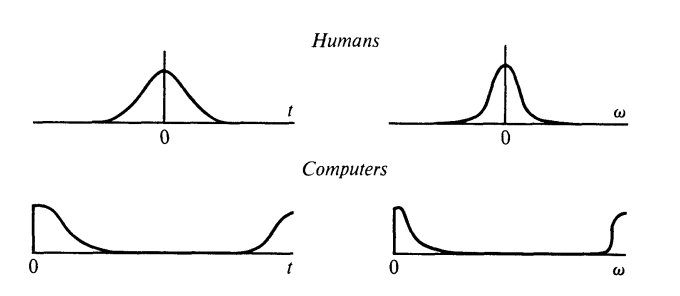
\includegraphics[width=0.5\textwidth]{xrf/human}
\caption[human]{一维傅氏变换程序的计算机内存安排}
\label{fig:xrf/human}
\end{figure}

试考虑对有八个点的时间函数进行一维傅氏变换。位于第一个向量元素的输出是零频
率,代表某一网格的、即函数$+1,-1,+1,
-1\ldots\ldots$的最高频率之Nyquist频率$\pi$是位于该八点
函数的第五个元素,其后伴随以负频率。最小的非零负频率位于第八个向量元素。如杲有第
九个元素,那么它会因周期性之故而等于第一个元素。偏移方法的输出不是实数,是初学者
的常见错误;采用单精度算法
时,虚部应为实部的$10^{-6}$左右,出
现与$1/N$呈正比(N为向量长度)的非常大的虚部,表明有程序错误。

下面是对二维程序的检查程
序,其中,“Write”语句是局部FORTRAN而不是Ratfor语
言。被变换的函数有几分像是时间轴上的某一种低频函数,而更多像是空间坐标轴上的某一种
低频函数。
\begin{minted}{Fortran}
\#Test case for two-dimensional Fourier Transformation

integer it,nt,ix, nx; complex cp(64,64), cwork(64) 
open(4,file= 'plotfile',status= 'new ',access= 'direct',form=
'unformat­ted', reel=l)
nx = 64; nt = 64; do it=l, nt
do ix=l, nx
	do ix=1, nx
		cp(it, ix) = 0.
cp(16,3)=1.; 
cp(16, 4) = 4.; 
cp(16,5)= 6. ; 
cp(16, 6) = 4.; 
cp(16, 7)=1.

cp(17, 3)=1.; 
cp(17, 4) = 4. ; 
cp(17, 5)=6. ; 
cp(17, 6) = 4. ;
cp(17, 7)=1.

call ft2d(nt, nx, cp, +1., +1., cwork)
write(4, rec=l)((real(cp(it, ix)), it=l, nt), ix=l, nx)
stop; end
\end{minted}
最基本的二维傅氏变换如下所示
\begin{minted}{Fortran}
2D Fourier transform by using ID program subroutine
ft2d(nl,n2,cp,signl,sign2,cwork) complex cp(nl,n2),cwork(n2) integer
nl,n2 real signl,sign2}

do i2 = l,n2 # transform over the fast dimension
call fork(nl,cp(l,i2),signl) #one-dimensional Fourier transform
do i 1 = l, n 1 { # transform over the slow dimension
do i2 = 1, n2
cwork(i2) = cp(il,i2)
call fork(n2,cwork,sign2) #one-dimensional Fourier transform
do i2 = l,n2
cp(il ,i2) = cwork(i2)
}
relurn; end

\end{minted}
最后,我们谈一谈一维快速傅氏变换程序。这一个程序是《地球物理数据处理基础》一
书第12页\footnote{中文译本的第19页,见1979年石油化学工业出版社出版之《地球物理数据处理基础》。——译者}上的FORTRAN语言子程序“fork”之Ratfor语言的翻版。照例,lx是2的整数
幂,输出cx(l)是零频率,cx(lx/2+
l)是所谓Nyquist频率,而cx(lx)则是最小负频
率。算法简短又策略,除非你参考其他的资料,你休想读得懂该程序。
\begin{minted}{Fortran}
# ID fast Fourier transform subroutine fork(lx,cx,signi)
complex cx(lx),carg,cexp,cw, ct j= 1 ; k= 1 ; sc = sqrt(l./lx)

do i = l,lx {

if(i<= j) {ct = cx(j) *sc; cx(j) = cx(i) *sc; cx(i) = ct}
m = lx/2

while(j>m) = m = m/2; if(m<l)break}

j = j + m
}
repeat {
istep=2 *k 
do m=l,k {

carg = (0., 1. ) * (3.14159265 *signi * (m-l))/k; cw = cexp(carg) do i =
m,lx,istep
{ct = cw *cx(i + k); cx(i + k)=cx(i)-ct; cx(i) = cx(i) + ct
}
k=istep
} until(k >= lx)
return; end
\end{minted}
傅氏变换既有实部又有虚部,有时二者均需显示。但往往是虛部略而不计,这是因为我们
用的时间函数大多数是在$t=0$
之前就已等于零了,所以,它们的傅氏变换必须满足一定的条
件,即实部与虚部必须是通过Hilbert变换而相互联系。狭义地说,
一个往往看起来像是余弦,
另一个看来像是正弦。因此,观察到实部,总是能
很容易想像出虚部。图\ref{fig:xrf/two-fourier}是检验程序的输出显示。
\begin{figure}[H]
\centering
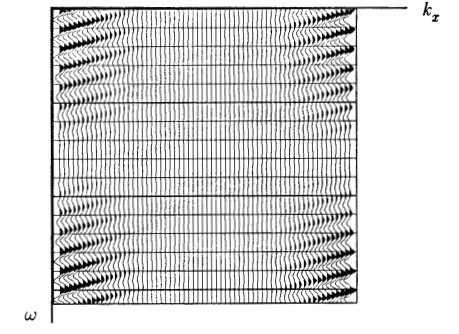
\includegraphics[width=0.5\textwidth]{xrf/two-fourier}
\caption[two-fourier]{二维傅氏变换检验程序的输出}
\label{fig:xrf/two-fourier}
\end{figure}
\subsection{Stolt偏移}
以下所示Stolt偏移程序采用线性内插方法将$\omega$轴转
换为$k_z$轴,用$dk_z/d\omega$进行标定,影响不太大,因而为
使程序简短而将它忽略不计了(对于习题,有些需要保留)。
实例检验的内容是根据脉冲作出半圆波阵面。
\begin{minted}{Fortran}
integer it,nt,ix,nx; real vdtodx; complex cp(256,64)
open(4, file = 'piotfile ',status='new * '.access =' direct
',form = 'unformatted recl = l)
nx = 64; nt = 256; vdtodx= 1./4. #vdtodx = v dt/dx

do it=l,nt
do ix= l, nx

cp(it,ix) = 0.

cp(32,9) = l.; cp(64,17) = 1. ; cp(l28, 33) = 1. 
call stolt(nt, nx, cp, vdtodx)

write(4,rec = l)((real(cp(it,ix)),it = 1, nt), i x = 1,nx)
stop; end

#Stolt migration subroutine without cosine weight.

subroutine stolt(nt,nx,cp,vdtodx)
integer ikx,nx,nt,nth,iktau,iom

real om,vkx,wl,wh,aktau,pi,pionth,vdtodx
complex cp(nt,nx),cbf(l025)

pi = 3. 14159265; nth = nt/2; pionth = pi/nth;

call ft2d(nt,nx,cp, 1. ,-l. ,cbf)

do ikx=l ,nx {

vkx = (ikx-l) * 2 * pi * vdtodx/nx

if(ikx > nx/2)vkx = 2.* pi * vdtodx-vkx #negative k_x

cbf( l) = 0. ; cbf(nt+1 = 0.  # cbf= working buffer

do iom=l,nt

cbf(iom) = cp(iom,ikx) # Omit weighting

cp( 1 ,ikx) = 0. # Ignore zero freq
do iktau = 2,nth+1 { # Stretch
aktau = (iktau-l.0l) *pionth
om = sqrt(aktau * aktau +vkx * vkx) ; iom= 1 +om/pionth
if(iom<nth) {
  wl = iom-om/pionth; wh=l.-wl
  cp(iktau, ikx) = wi * cbf(iom) + wh * cbf(iom +1)
  cp(nt-iktau + 2, ikx) = wl * cbf(nt-iom + 2) + wh * cbf(nt-iom+1)
}
else
cp(iktau, ikx) = 0.
}

call ft2d(nt,nx,cp,-l. , 1. ,cbf) 
return; end
\end{minted}
这种检验程序的输出曾经在1.3节内显宗过,为棱好地阐明解的周期性质,其余一个半
圆波阵面外所有其他均已消除了,而且该输出结果是按非线性增益来显示的。图\ref{fig:omk/stolt4}中逐
端相接出现的是四个相同图形。
\begin{figure}[H]
\centering
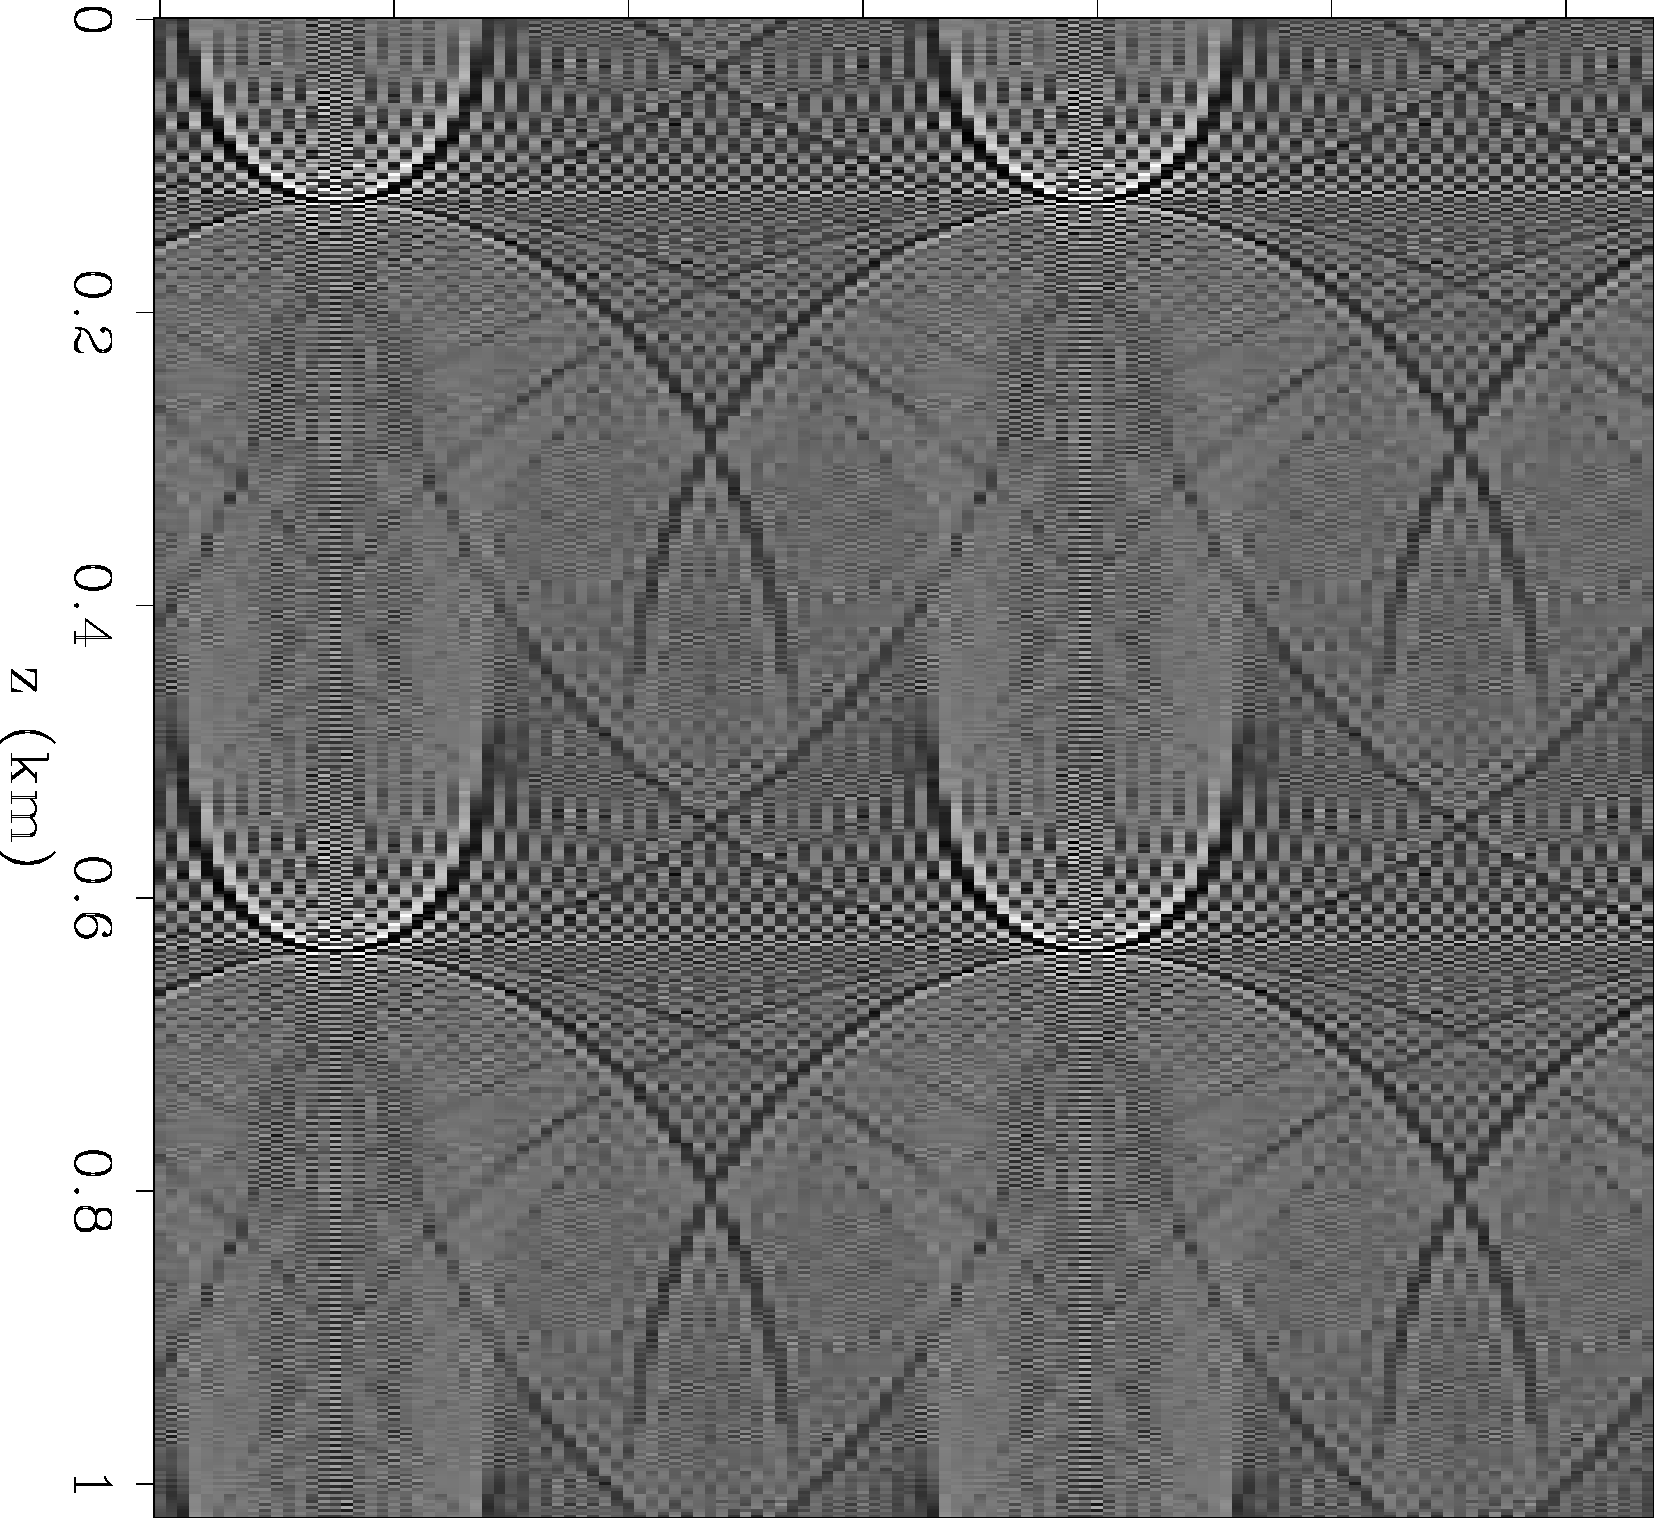
\includegraphics[width=0.5\textwidth]{omk/stolt4}
\caption[stolt4]{Stolt偏移程序输出的周期性}
\label{fig:omk/stolt4}
\end{figure}
\subsection{Rocca的按行傅氏变换}
Rocca的按行傅氏变换比原始程序要快速一点,因为基本的一般性运算是一次完成,而
这时每行均实现了傅氏变换。但是Rocca方法超过原始方法的主要优点在于不需数据的转
置,而且即使在按页读的条件下该程序也能有效地运行。
\begin{minted}{Fortran}
#Try Rocca's row Fourier transform.
# sign2 should be+l.or-l.it is the sign of i. 
subroutine rowcc(nl,n2,cx,sign2,scale) 
complex cx(nl,n2),cmplx,cw,cdel 
do il =l,nl do i2=l,n2
cx(il,i2)= cx(il,i2)* scale
doi = 1,n2 {
if(i <= j) call twidl(nl,cx(l,i),cx(l,j))
m = n2/2
while(j>m) {j = j-m; m = m/2; if(m<1)break}
j = j + m } 
istep = 1
repeat {
istep = 2 * istep; cw = i.
arg=sign2 *3.14159265/istep;} cdel = cmplx(cos(arg),sin(arg))
do m=l,istep {
do i = m,n2,istep
call twid2(n 1, cw, cx( 1, i), cx( 1,i + lstep)) 
cw = cw * cdel
istep = istep } until(istep>=n2) 
return; end

subroutine twidl(n,cx,cy) 
complex cx(n),cy(n),ct
doi=l,n {ct = cx(i); cx(i) = cy(i); cy(i) = ct}
return; end

#If you feel like optimizing,this is the place, 
subroutine twid2(n,cw,cx, cy) 
complex cx(n),cy(n),ctemp,cw
do i = l,n {ctemp = cw*cy(i); cy(i) = cx(i)-ctemp; cx(i) = cx(i)+ ctemp} 
return; end
\end{minted}
\subsection{习 题}
\begin{enumerate}
\item 大多数时间函数均属实函数,其虚部为零。试证:这意味着$F(\omega,k)$可由$F(-\omega,-k)$确定。
\item 利用你的计算机和图形显示仪,试检验图\ref{fig:xrf/two-fourier}是用所给出的程序作出的。

\item 前一题中所显示的傅氏变换之实部有点难以解释,因为负频率与负波数的处置很棘
手。试修正该程序使$F(\omega,k)$的原点位于显示网格的中心(33,33)。提示:在进行傅氏变换之前简单修改$f(t,x)$就行了;回想一下“时移定理”。写出$f(t,x)$和新的更容易
解释的$F(\omega,k)$,标明坐标轴。
\item 时间$t=0$时在地表面位于$x=32$之处的点源爆炸得出的在$(t,x)$平面内之合成观
测结果如下面\ref{fig:dft/airwave}左图所示。右图是$(\omega,k_x)$平面上的二维傅氏变换之量值。每张图的原点位
于各该图的左上角。试问在速度值降低一半的地层中这些图看上去会是什么样子?
\begin{figure}[H]
\centering
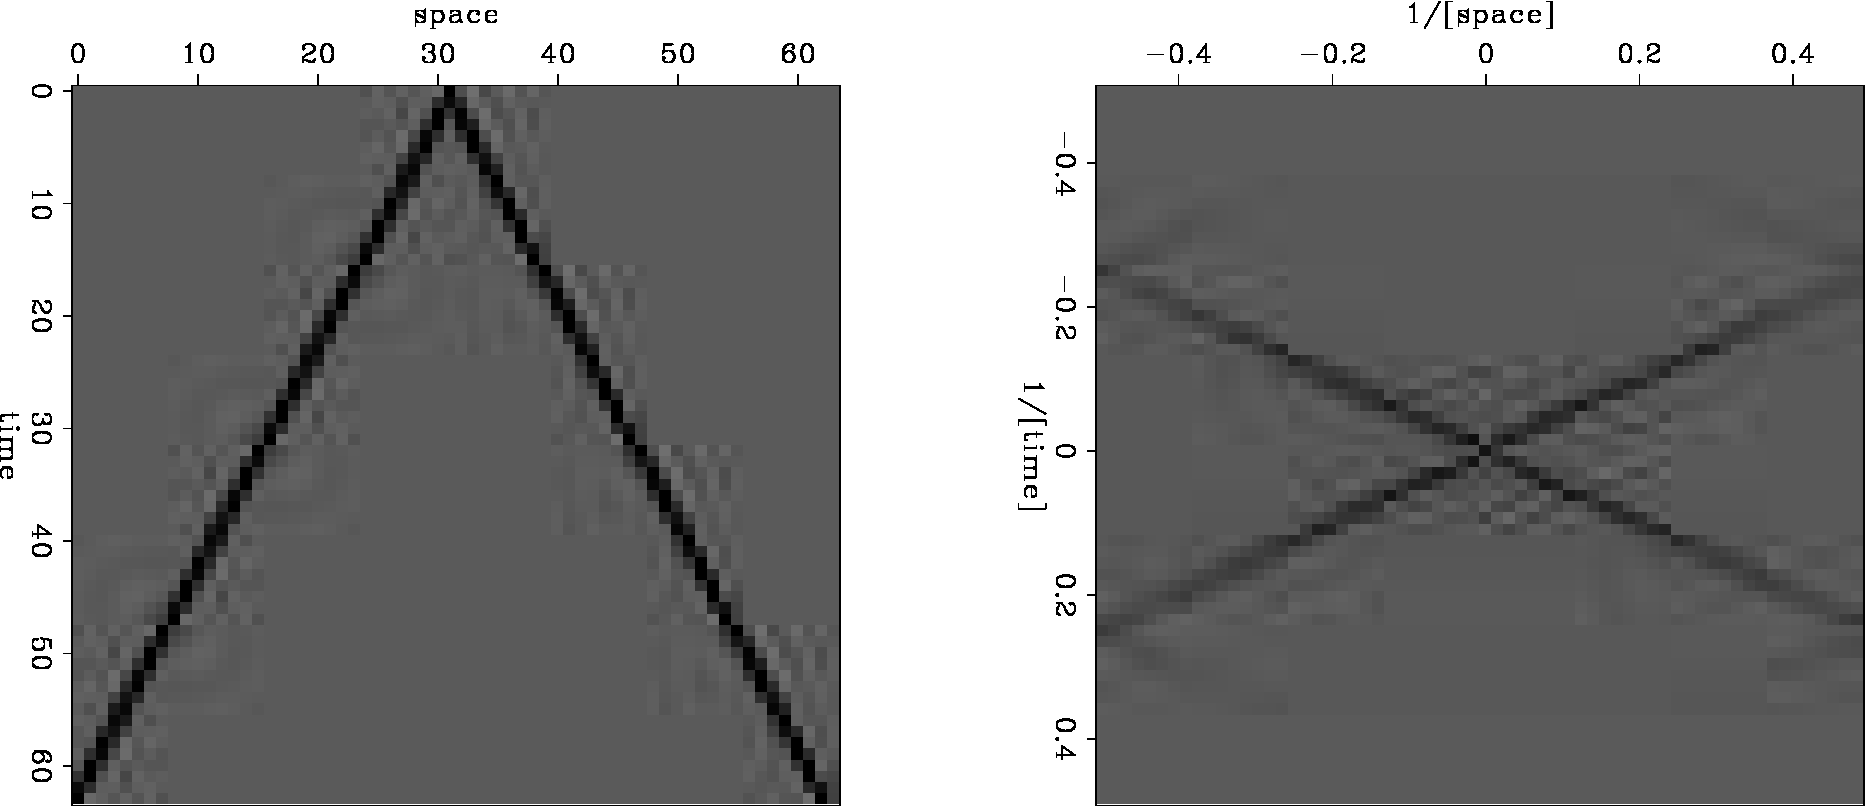
\includegraphics[width=0.95\textwidth]{dft/airwave}
\caption[airwave]{习题4}
\label{fig:dft/airwave}
\end{figure}
\item 在Stolt偏移程序中插入适当的余弦倾斜因子函数。试检验并证明除某种有角度依
赖关系的比例因子之外,差异很小。
\item 根据Stolt方法,写一个绕射程序。就是说,已知地层内的点散射体,试用该程序
作出适当的双曲线。
\item 当你使Stolt绕射程序内包括有余弦加权函数的倒数时,要谨防在尖灭边缘上有极
点存在。试问在加权之前还是在加权之后进行拉伸处理才比较妥当?为什么?
\item 使$P(\omega)$随$\omega$的振荡速率减小就能够减少Stolt程序之内插误差,这么处理时要注意
$p(t)$对于负$t$应等于零。因此,在内插之前用$e^{-i\omega\tau}$乘$P(\omega)$,然后在内插以后又用它来
除。试问:程序中采用的常数$\tau$应取什么合适的值?
\end{enumerate}


\chapter{为何采用时空域处理}
\label{chap:why-time-space}

前一章讨论了如何将波场向下外推,进行外推处理很简单,因为它只不过是在频率域内
用$\exp[ik_z(\omega,k_x)z]$来乘而已。有限差分法则较复杂,这将涉及新的近似和新的陷阱。
我们为何要自寻烦恼去学习它呢?首先,许多人发现有限差分方法更易于理解,在时间空间
域$(t,x,z)$内,没有复数,没有复指数,也没有称为FFT
(快速傅氏变换)的“魔盒”。

情况类似于在普通的频率滤波中所遇到的情形。频率滤波可以作为频率域内的某种乘积
或者时间域内的某种褶积来完成,而波场外推则既有与时间有关的频率域$\omega$内的乘积又有与空
间有关的波数域$k_x$内的乘积。新因素就是二维$(\omega,k_x)$空间,它代替了旧有的一维$\omega$空间。
关于为什么要自找麻烦去利用有限差分这个问题,其实是一个涉及为何要采用二维形式的老
问题:在已经发现快速傅氏变换以后,为什么还要用时间域滤波运算去自找麻烦呢?

在许多场合下还会多次提出这个问题。以后我们还会有炮检距坐标轴和共中心点坐标
轴,所以我们还需要选择究竟是在这些坐标上应用有限差分法呢还是采用傅氏变换。这不是
一种要么全是要么全非这样的命题:不是必须选择傅氏变换,就是必须选择褶积(有限差
分)。

这个问题的答案是多方面的,正如地球物理目标是多方面的一样。判断该问题答案是否正
确的准则大多数是从普通的滤波理论中所早已熟知的。那些电气工程师和曾经强迫自己涉足
波动处理领域的老式反褶积专家到头来是要为这一点而深感高兴的,他们未曾料到他们的知
识竟已经有了这么多方面的应用。

图\ref{fig:txz/freqhyp}说明傅氏变换域计算与时间域计算之间的差异。为突出显示各个域内都有难点,
该图是在一种$256\times64$的网格上计算出来的。一般来说,你可注意到在傅氏域计算中有假频干
扰,在时间域计算中有频散(见\label{sec:4.3}节)。(图\ref{fig:txz/freqhyp}中的所谓“时间域”双曲线实际上就
是频率域情形的一种重复模拟——将整个双曲线叠合起来进入视界)。在本章中,我们将会知
道如何去完成时间域计算,各个域内计算结果的更详细比较在第四章内进行。
\begin{figure}[H]
\centering
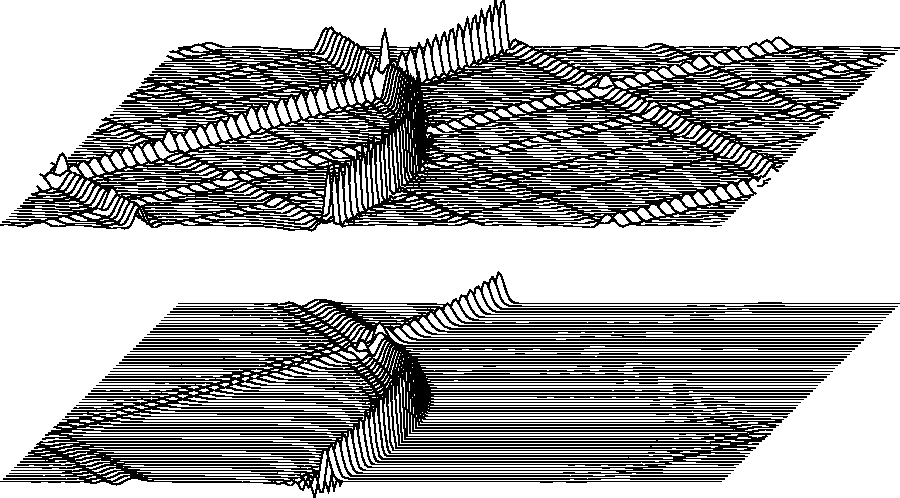
\includegraphics[width=0.95\textwidth]{txz/freqhyp}
\caption[freqhyp]{频率域双曲线(上图)与时间域双曲线(下图)}
\label{fig:txz/freqhyp}
\end{figure}

即使你经常在频率域内作偏移处理,为有助于你选择参数以获得良好时间域响应,研究
一下时间域方法还是值得的。例如,图\ref{fig:txz/freqhyp}的上、下两部分都是在频率域内完成的,但是
为获得更合理的响应,有一种是模拟时间域计算的。
\subsection{横向变化}
在通常的线性滤波理论中,一个滤波器可以成为时变的,这点在反射地震学中很有
用,因为回声反射的频率成分就是随时间而改变的。时变滤波的一个恼人问题是不能用频率
域内的简单乘积关系描述它,所以在时变滤波是单独应用时,就得放弃频率域,或者,就得构
造出所有类型的畸变(例如,对时间坐标轴进行拉伸)以便显得像是时变的。

所有这些考虑同样也适用于水平空间坐标二关于空间坐标,还涉及一个新问题,这就
是地震波速度$v$。如果速度是空间可变的,例如是$v(x)$,则向上和向下外推波场的运算就
不能表示为$k_x$域内的乘积关系了,进行波场外推必须放弃空间频率域而采用有限差分。为显
得像是空间可变(space-invariant),可供选择的办法再一次又是构造一切类型的畸变(诸
如对$x$轴进行拉伸之类)。

在二维或二维以上的情形下,进行拉伸处理会变得更困难而且很少能令人满意。

建议采用有限差分而不采用傅里叶变换方法。还有一种问题类型相同但情况不那么严峻
的原因,那就是记录道位置的空间横向变动。如检波器由于某种原因变成了不规则分布,致
使记录道间距$\Delta x$不是与$x$无关,这时就只有两种办法可供选择了 :
\begin{enumerate}
\item 在进行傅里叶分析
之前,以均匀间隔对数据进行重采样;
\item 用有限差分直接处理资料。
\end{enumerate}

\subsection{时差}
许多地震学方法是进行时移测定。时差(Stepout)
一词表示旅行时间随位置之改变而
发生的变化。通常频率域的计算结果最后都要变换至时伺域,以便时移清楚可见。时间域计
算的好处就是:在进行计算时就可以测定波束的时移。在频率域内,确定一个时间参考点或者
描述整个时间函数的时间偏移倒并不困难,但是不变换返回时间域就想存取单独的子波或波
束就没那么容易。

上行波场和下行波场的外推滤波因子、即$\exp[ik_z(\omega,k_x)z]$,基本上是一种物理可
实现全通滤波(在某些情形下,它是非物理可实现的),它可以完成能量偏移而无放大或阻
尼作用,我想这就是为什么偏移滤波比极小相位滤波更有意思的原因。偏移滤波遍及所有空
间采集能量而后置于恰当的位置上,而极小相位滤波则完全难以使能量偏移,它们只不过
是使某些频率成分放大而使另外一些频率成分缩小而已。任何形式为$\exp[i\phi(\omega)]$的滤波因
子都是一种全通滤波(all-pass filter),那么,欲使$\exp (i\phi)$的时间域表现形式具有物
理可实现性,函数$\phi(\omega)$到底应有什么约束条件呢?

物理可实现全通滤波具有一种颇引人注意的表现形式,用Z变换来描述,就是具有
$Z^N\overset{-}{A}(l/Z)/A(Z)$形式。熟悉滤波理论的人都会理解,用来除要涉及到一系列新
问题:反馈、参量简化以及可能的不稳定性(见\ref{sec:4.6}节关于Z变换的讨论)。在采用有限差
分进行波场向下外推时,同样也会引起所有这些问题。向下外推就是一个反馈过程。参量简
化是颇引人入胜的,设取$A(Z)=1+a_1Z+a_2Z^2$,有两个可调节的系数就足以为有选择的延
迟选出适当的频率和频带宽度了。参量简化也意味着应用时很省事,这点是很妙的。很妙的
还有:所具有的函数形式本身就意昧着具有物理可实现性。另一方面,节省时间所能带来的
好处会被若干危险因素所抵销,所以我们现在必须熟悉并利用某种稳定性定理,必须假定
是极小相位的。

\subsection{频率域内消除干扰要求过苛}
傅里叶方法是整体性方法,就是说,在可以开始进行处理之前,必须掌握有全部数据
组。间接误差与截断误差可能具有严重的局部影响。另一方面,有限差分方法则是局部性方
法,各数据点仅与其邻点直接有关,间接误差传播缓慢。让我们在一维时间序列分析方面举
出两个有关频率域隐藏危险的例子。

在频率域内很容易设计锐截止滤波因子,例如,设计成在8赫兹至80赫兹之间有一绝对平
坦的通频带而在其外则一律为零。但这类滤波因子在时间域内却引起了问题,它们必然是非
物理可实现的,即在能量输入于滤波器之前就产生响应。另一个糟糕的问题是时间响应只随
时间t反比衰减。这样一来,振幅已按时间平方反比衰减的到达较迟之深反射就将被较早到
达之反射所引起的长长的滤波响应所淹没。

更常见的问题是由抑制60周动力线频率的滤波器引起的,许多记录设备中均有这类滤波
器。在Z变换域内很容易设计这类陷频滤波器,只需在单位圆上准确等于60周之处有一个零
点即可。这种滤波器可消除60周干扰,但是它却会在其他频率上使通频带畸变。因此,需要
在单位圆之外稍远的地方置一极点。极点与零点之间的间距决定了陷频的频带宽度。如从单
位圆周上某种距离之处来观察这一对点时,该极点就具有几乎将零点影响完全消除的作用。
因此,远离抑制带就有理想的平缓频谱。你就用这种滤波器来记录某种数据。由于到达晚的
反射均比到达早的一些反射要弱些,所以,显示绘图程序就得随时间而增大其增益。但在接
入你的陷频滤波器后,你会发现这种滤波器使动力线干扰增大了而不是减弱了。为什么?原
因就在于你企图过于干净地消除干扰而使极点过于靠近零点了。指数增益实际上使单位圆远
离零点而移向极点,于是极点也许就落在了单位圆上!使极点远离零点可形成一种比较开阔
的陷频带,在频率域内设计滤波器时,这点是不受欢迎的,但是当增益随时间而变动时,这
种滤波器至少会工作得比较灵敏。

\subsection{填补零值点}
开始应用快速傅氏变换时,首先是应用于褶积。如果一个滤波因子有多于五十项左右的
系数,用频率域内的乘法来实现该项滤波处理,运算速度会比较快一些。如已经谨慎地用足
够的零值点填满了数据与滤波因子的尾端部分,这种运算结果将与褶积结果完全相同。填补
零值点使离散傅氏变换的周期性质被掩盖起来而不露痕迹。对典型长度约为一千个采样点的
时间函数进行滤波时,为了节省计算时间,宁可稍许增加一些内存,而地震剖面都是有上千
记录道之长的。对于偏移运算,必须同时在空间轴与时间轴上完成零值点的填补。可能需要
补零的有三处,如下所示:
\begin{table}[!ht]
\centering
\ttfamily
\small
\begin{tabularx}{\textwidth}{|Y|Y|}
%\begin{tabular}{p{3cm}p{4cm}p{4cm}p{5cm}}
%\toprule
\hline
 数据& 0 \\
%\midrule
\hline
0&0\\
\hline


%\bottomrule
\end{tabularx}
%\end{tabular}
\end{table}
在\ref{sec:4.5}节内将对如何减轻频率域偏移的麻烦问题有所提示。

\subsection{展望}
频率域内的一些问题已在上面总结过了,在这一章和第四章内,将要指出空间域内存在
的一些问题。地震数据处理是一种多维的处理任务,而不同的维数往往要用不同的方法去处
理。不过,如果你确信你对于频率域处理有把握,那么,你可以将这章的很多部分跳过而直接
去阅读第三章。在该章中,你可学习到有关炮检距、叠加及叠前偏移等问题。



\section{波场外推方程}
波场外推方程是一个有关波场之导数(通常是沿深度$z$的方向)的表达式。当已知波场
及其导数时,就可利用$P(z+\Delta z)=P(z)+\Delta zdP/dz$的各种不同数值表示方法来处理外推问
题,所以真正需要的是有关$dP/dz$的表达式。求解$dP/dz$的两种理论方法是早期的变换方法
和较新的波散关系方法。

\subsection{抛物线型波动方程}
在抛物线型方程被引用于石油勘探的时期(1969年),“波动理论不起作用”这种论调
相当流行。在那个时代,石油勘探人员分析地震资料是采用射线方法,波动方程还与实际工
作无缘,唯有大学里的理论家们才会问津波动方程(事实上,波动理论对于比地震勘探尺度
大一千倍的大规模天然地震中的面波,是起过作用的)。即使是大学的研究人员,那时也未
曾完善地建立波动方程的有限差分解,计算机是计算机,解是解,所解决的多为“鼓面振
动”之类的问题,而不是求解“地层中传播的地震波”
。最早是为了提高有限差分波动模拟
的计算效率而才引入抛物线型波动方程,下面对抛物线型波动方程的介绍就是藉助于原来采
用的变换方法。

1969年以前,困难来自于有一个对当时所有地震波理论极为重要而又不恰当的假设,即
水平成层假设。射线追踪曾是摆脱该种假设限制的仅有方法,但采用射线追踪看来就得放弃
地震波形的模拟。在石油勘探中,几乎所有波动理论其本身更进一步还得受垂直入射的限
制。成功地克服困难的途径就在于将垂直入射情形加以推广,沿垂直入射方向周围允许有微
小角度变化范围,放弃许多熟悉但很麻烦的地震理论就达到了这个目的。

垂直下行平面波在数学上以下述方程表示
\begin{equation}
P(t,x,z)=P_0e^{-i\omega (t-z/v)}
\label{eq:ex2.1.1}
\end{equation}
式中,$P_0$纯为常数。将$P_0$用某种不是严格恒定而是缓慢变化的函数$Q(x,z)$来代替,即可
模拟偏离垂直入射的微小角度改变,即
\begin{equation}
P(t,x,z)=Q(x,z)e^{-i\omega (t-z/v)}
\label{eq:ex2.1.2}
\end{equation}
将式\ref{eq:ex2.1.2}代入标量波动方程$P_{xx}+P_{zz}=P_{tt}/v^2$,得
$\frac{\partial^2 Q }{\partial x^2}+(\frac{i\omega}{v}+\frac{\partial}{\partial z})^2Q
=-\frac{\omega^2}{v^2}Q$
即
\begin{equation}
\frac{\partial^2 Q }{\partial x^2}+\frac{2i\omega}{v}\frac{\partial Q}{\partial z}+\frac{\partial^2 Q}
{\partial z^2}=0
\label{eq:ex2.1.3}
\end{equation}
导出此式时,未作任何假设,仅仅是将波动方程用$Q(x,z)$重新加以表示而已。为使波场接近于平面波,$Q(x,z)$
必须接近于一常数。适宜的假设应是$Q$沿深度的最高阶导数、即$Q_{xx}$可忽略不计(首次引入这个假设时,曾引起一些争论),这就使我们得出抛物线型波动方程
\begin{equation}
\frac{\partial Q }{\partial z}=-\frac{v}{2i\omega}\frac{\partial^2 Q }{\partial x^2}
\label{eq:ex2.1.4}
\end{equation}
首次建立这个方程用于地震学的时候,当时认为式\ref{eq:ex2.1.4}的最重要性质是这样一
点:对于接近于沿垂直方向传播之平面波的,一种波场而言,沿$x$轴方向的二阶导数应很小,
因而沿$z$轴方向的导数应很小。所以,应用有限差分方法时将允许采用非常大的步长$\Delta z$,从
而能使处理的模型更像是地层模型而不大像是鼓面。

随后,很快就弄明白了,抛物线型波动方程也正是地震成像方法所需要的那种方程,即
它是一种波场外推方程。

妙极了,式\ref{eq:ex2.1.4}就是量子力学中的Schroedinger方程的形式。

这种办法、即变换方法曾经是而且现在也是非常有用的。不过它很快就为波散方程处理
方法所取代,这是获得以较宽角度进行波场外推的方程的途径。
\subsection{Muir平方根展开方法}
在我们采用较新的求解波场外推算子的方法时,要探索平方根波散关系的各种不同近
似,然后,将近似波散关系反变换为一个偏微分方程。自从我的《地球物理数据处理基础》
一书写成以来,波散关系处理方法已经有了显著进展,这得大大感谢Francis
Muir。

将平面波$exp(-i\omega t+ik_xx+ik_zz)$代入二维标量波动方程,得出波散关系
\begin{equation}
k_x^2+k_z^2=\frac{\omega^2}{v^2}
\label{eq:ex2.1.5}
\end{equation}
求解$k_z$,选择正平方根(选择下行波时即如此)
\begin{subequations}
\begin{equation}
k_z=\frac{\omega}{v}\sqrt{1-\frac{v^2k_x^2}{\omega^2}}
\label{eq:ex2.1.6a}
\end{equation}
为沿$z$轴进行反变换,我们仅需理解相应于反变换所得最终表达式是一个波
场外推算子,即
\begin{equation}
\frac{\partial P}{\partial z}=i\frac{\omega}{v}\sqrt{1-\frac{v^2k_x^2}{\omega^2}}P
\label{eq:ex2.1.6b}
\end{equation}

\end{subequations}
将方程\ref{eq:ex2.1.6b}变换回空间域并非就是用一个有关$x$的二级导数代换$k_x^2$这么简单的
事,问题是微分算子之平方根的意义何在。大学的微积分教程并未解释微分算子平方根的意
义,因而没有直截了当的有限差分表达式。仅在该平方根被看成是某种类型的截断级数
展开时,以$ik_x=\partial/\partial x$
来代表沿$x$方向的反变换才变得有章义。\ref{sec:4.6}节将证明,选择Taylor级
数展开并不是好办法。Francis
Muir曾指出,原有的15°与45°偏移外推法都正好是一种连分
式展开式的截断。为话明这点,设将式\ref{eq:ex2.1.6a}写成下列形式以定义出$X$与$R$
\begin{equation}
k_z=\frac{\omega}{v}\sqrt{1-X^2}=\frac{\omega}{v}R
\label{eq:ex2.1.7}
\end{equation}
所希望的$n$阶多项式比值将以$R_n$表示,按照下列递推关系
\begin{equation}
R_{n+1}=1-\frac{X^2}{1+R_n}
\label{eq:ex2.1.8}
\end{equation}
来确定该比值。为了解这种序列的收敛情形(如果它收敛的话),在式\ref{eq:ex2.1.8}内令$n=\infty$
从而解出
\begin{gather}
R_{\infty}=1-\frac{X^2}{1+R_{\infty}} \notag \\
R_{\infty}(1+R_{\infty})=1+R_{\infty}-X^2 \notag \\
R^2=1-X^2
\label{eq:ex2.1.9}
\end{gather}
式\ref{eq:ex2.1.9}的平方根给出所要求的表达式\ref{eq:ex2.1.7}。从几何意义来说,式\ref{eq:ex2.1.7}说
明:入射角余弦之平方等于1减正弦之平方。将展开式截断要产生角度误差。事实上,经常
采用的只是展开式中的低阶项,从$R_0=1$开始,求出其结果如表\ref{tab:2.1.1}所列
\begin{table}[!ht]
\centering
\ttfamily
\small
\begin{tabularx}{\textwidth}{Y|Y}
%\begin{tabular}{p{3cm}p{4cm}p{4cm}p{5cm}}
%\toprule
\hline
$5^{\circ}$& $R_0=1$ \\ \hline
$15^{\circ}$& $R_1=1-\frac{X^2}{2}$ \\ \hline
$45^{\circ}$& $R_2=1-\frac{X^2}{2-\frac{X^2}{2}}$ \\ \hline
$65^{\circ}$& $R_3=1-\frac{X^2}{2-\frac{X^2}{2-\frac{X^2}{2}}}$ \\ \hline

%\bottomrule
\end{tabularx}
%\end{tabular}
\caption{Muir连分式展开的头四项截断式}
\label{tab:2.1.1}
\end{table}
由于各种历史的原因,表\ref{tab:2.1.1}所列各方程往往分别称为5°、15°和45°的方程,对于可
充分掌握的角度范围而言,这些名称能给出合理的定性说明(但定量上是粗劣的)。为兼顾
构造复杂性和计算精确度,经常是指定选择45°方程。后来搞清楚了,要是从$R_0=cos45^{\circ}$这
类的值开始递推计算,可容纳的角度范围还可以再稍微宽一点。热衷于提高精确度的人也许
可使及。是一个速度的、空间坐标的或者频率的函数。
\subsection{波散关系}
为与准确的表达式\ref{eq:ex2.1.6a}比较起见,将表\ref{tab:2.1.1}所列展开式代入式\ref{eq:ex2.1.7}内,得出波散关系如表
\ref{tab:2.1.2}所示。如图\ref{fig:omx/disper}所示,表\ref{tab:2.1.2}的波散关系均趋近于半圆。
\begin{table}[!ht]
\centering
\ttfamily
\small
\begin{tabularx}{\textwidth}{Y|Y}
%\begin{tabular}{p{3cm}p{4cm}p{4cm}p{5cm}}
%\toprule
\hline
$5^{\circ}$& $k_z=\frac{\omega}{v}$ \\ \hline
$15^{\circ}$& $k_z=\frac{\omega}{v}-\frac{vk_x^2}{2\omega}$ \\ \hline
$45^{\circ}$& $k_z=\frac{\omega}{v}-\frac{k_x^2}{2\frac{\omega}{v}-\frac{vk_x^2}{2\omega}}$ \\ \hline
\end{tabularx}
%\end{tabular}
\caption{波散关系}
\label{tab:2.1.2}
\end{table}
\begin{figure}[H]
\centering
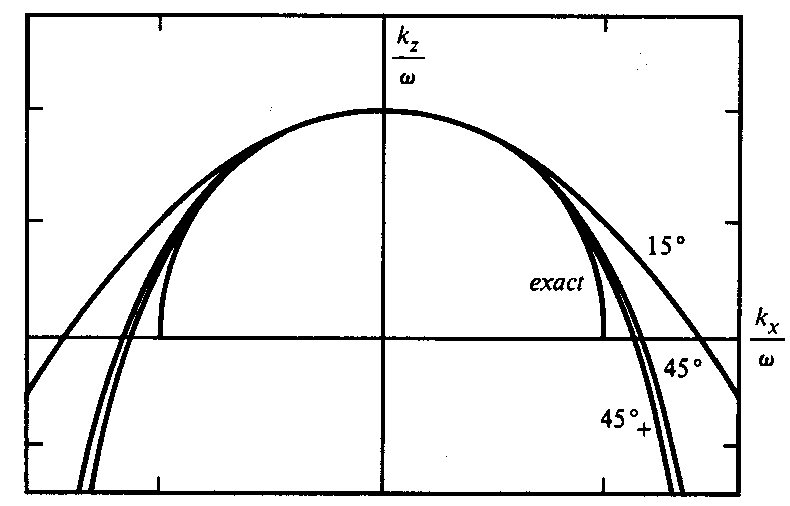
\includegraphics[width=0.6\textwidth]{omx/disper}
\caption[disper]{表\ref{tab:2.1.2}与式\ref{eq:ex2.1.6a}所示波散关系。标有$45_{+}^{\circ}$的曲线系按$R_0=cos45^{\circ}$构制,它准确地拟合于$0^{\circ}$和$45^{\circ}$的情形}
\label{fig:omx/disper}
\end{figure}
\subsection{速度随深度而变化的情形}
以算符$\partial /\partial z$代替$ik_z$可将表\ref{tab:2.1.2}的波散关系转换成表\ref{tab:2.1.3}所示偏微分方程。
\begin{table}[!ht]
\centering
\ttfamily
\small
\begin{tabularx}{\textwidth}{Y|Y}
%\begin{tabular}{p{3cm}p{4cm}p{4cm}p{5cm}}
%\toprule
\hline
$5^{\circ}$& $\frac{\partial P}{\partial z}=i[\frac{\omega}{v}]P$ \\ \hline
$15^{\circ}$& $\frac{\partial P}{\partial z}=i[\frac{\omega}{v}-\frac{vk_x^2}{2\omega}]P$ \\ \hline
$45^{\circ}$& $\frac{\partial P}{\partial z}=i[\frac{\omega}{v}-\frac{k_x^2}{2\frac{\omega}{v}-\frac{vk_x^2}{2\omega}}]P$ \\ \hline
\end{tabularx}
%\end{tabular}

\caption{速度仅与深度有关时的外推方程}
\label{tab:2.1.3}
\end{table}
表\ref{tab:2.1.3}各偏微分方程均以某个波散关系为基础,因而到头来都是以一种恒定速度假设为
基础。所以,你不能指望在速度随深度而变化时、即$v=v(z)$时方程还能有重要的应用价值或甚至还有很大用处。它们本身是无能为力描述反射的,这正好说明了它们的实际限度。

以式\ref{eq:ex2.1.6b}或表\ref{tab:2.1.3}所示各式为基础的偏移方法均称作相移法。
\subsection{延迟频率域}

\section{有限差分}
有限差分是计算机求解微分方程的基本方法,这神方法的最佳特点就是它可以分析几乎
任何形态的对象、诸如大地地形或地质构造等。进行差分计算通常是一种简单的任务,其主
要问题是不稳定性。往往发生这样的现象,对一个合理的物理问题看来是合理的处理方法却
导致剧烈振荡和不收敛的计算结果。幸好,还有十分稀少的一些重要而又易于掌握的技巧可
以解决大多数不稳定性问题。

具有次要意义的一些问题是计算时间与精度问题。由于要付出更精细计算网格这样的高昂
代价方可改善精度,所以必须将计算时间与精度二者综合加以考虑。虽然选择以下几节所述方
法并非出于对猜度或计算效率的考虑,不过在这些领域内,这些方法确实是出色的。说实在的,
据我所知,某些方法完全不可能再改进了,而另一些方法改进的余地则可能很小。所谓“小”,
我的意思是指效率提高不超过五倍的改进。这样的改进很少是由于研究或试验工作的结果。
然而,鉴于它对生产工作具有重要性,进一步阅读远超出以下几节内容的文献还是很必要的。

\subsection{透镜方程}
各种波场外推算子均可分为两部分:较复杂的部分称为绕射或偏移部分,而较简单的部
分则称作透镜部分。透镜方程引入了一个作为$x$之函数的时移,由于它正像一个光学薄透镜
在光线沿轴向投射(垂直投射)时那样起作用,故而获得透镜方程这种名称。在绕射部分
中,以某种方式隐含着对非垂直入射和透镜厚度的校正.透镜方程存在有解析解,即$\exp[i\omega t_0(x)]$
。运算时,最好是利用这种解析解而不是利用某种差分解,因为解析解没有因采用近
似计算而引起的误差。在讨论有限差分的一章中之所以会提到透镜方程,其仅有的原因完全是
由于伴随的绕射方程必须与透镜方程一起向前推进计算,所以解析解要沿很小的步长推进。

\subsection{一次导数与显式方法}

速率为10\%的通货膨胀率$q$可用下述差分方程描述
\begin{subequations}
\begin{equation}
q_{t+1}-q_t=0.10q_t
\label{eq:2.2.1a}
\end{equation}
\begin{equation}
(1.0)q_{t+1}+(-1.1)q_t=0
\label{eq:2.2.1b}
\end{equation}
\label{eq:2.2.1}
\end{subequations}
这类一维计算可用差分系数表和数据表重新加以表示,就这一点而论,它对如何组织二维偏
微分方程的计算提供了一种范例。设有下列系数表与数据表
\begin{figure}[H]
\centering
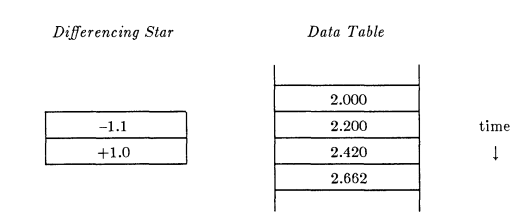
\includegraphics[width=0.5\textwidth]{new/datatable}
\caption[datatable]{差分系数表和数据表}
\label{fig:new/datatable}
\end{figure}
由于数据表中的数据满足差分方程\ref{eq:2.2.1},可将差分系数表置于数据表顶部的任何地
方。将系数表中的数乘以它下面的表中的那些数,所得互乘结果之和将为零。另一方面,如
果数据表中除一个数(初始条件)之外,所有的数都没有,则可沿时间増大方向滑动该系数
表。取互乘之和并令差分方程成立,一次计算出一个数,每一步都可解出未知数据值,从而
可将数据表中所有其余的数部填满。

当数值系数0.10周一个复数代替时,利用同一套差分系数表就要稍为繁琐一些。这种情
形下,计算结果既表现出有振荡现象,又表现出有增大和阻尼衰减的现象。

\subsection{一次导数与隐式方法}
试以数值方法求解下述方程:
\begin{equation}
\frac{dq}{dt}=2rq
\label{eq:2.2.3}
\end{equation}
注意,在通货膨胀方程\ref{eq:2.2.1}中是$2r=.l$,那种方程是一种近似式,但是现在要注意,在
通货膨胀方程中的表达式$dq/dt$是位于时间$t+1/2$,而表达式$q$本身则位于时间$t$。没有理由
不把式\ref{eq:2.2.3}右端的$q$在时间$t$上用时间$t+1$来加以平均,因而可将整个方程均置于时间
$t+1/2$。具体说,式\ref{eq:2.2.3}的中心差分近似为
\begin{subequations}
\begin{equation}
q_{t+1}-q_t=2r\Delta t\frac{q_{t+1}+q_t}{2}
\label{eq:2.2.4a}
\end{equation}
令$\alpha=r\Delta t$,上式变为
\begin{equation}
(1-\alpha)q_{t+1}-(1+\alpha)q_t=0
\label{eq:2.2.4b}
\end{equation}
\label{eq:2.2.4}
\end{subequations}
\begin{figure}[H]
\centering
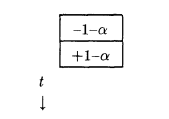
\includegraphics[width=0.25\textwidth]{new/difftable}
\caption[difftable]{差分系数表}
\label{fig:new/difftable}
\end{figure}
在固定步长的情形下,这种系数表得出的微分方程\ref{eq:2.2.3}的解比前述由通货膨胀系数表得出的解更为精确。

\subsection{显式热流方程}
热扩散系由热流方程控制.这种方程是地震偏移方法的一个原型,15°偏移方程与该方
程形式相同,只不过热传导常数是虚数而已(偏移方程实际是Schroedinger方程,该方程
描述原子粒子扩散几率)。取$\sigma$为常数,得热流方程
\begin{equation}
\frac{\partial q}{\partial t}=\frac{\sigma}{c}\frac{\partial^2 q}{\partial x^2}
\label{eq:2.2.5}
\end{equation}
在计算机上实现式\ref{eq:2.2.5}的计算需对各偏微分作某种差分近似。最明显不过(但并非
唯一的)的办法就是采用初等微积分教程中关于微分的基本定义,就时间导数而言,这就
是
\begin{subequations}
\begin{equation}
\frac{\partial q}{\partial t}\approx \frac{q(t+\Delta t)-q(t)}{\Delta t}
\label{eq:2.2.6a}
\end{equation}
利用下标使式\ref{eq:2.2.6a}形式紧凑是很方便的
\begin{equation}
\frac{\partial q}{\partial t}\approx \frac{q_{t+1}-q_t}{\Delta t}
\label{eq:2.2.6b}
\end{equation}
\end{subequations}
在这种符号表示中,$t+\Delta t$简记为$t+1$,对于更为复杂的方程有其方便之处。取两次一阶导
数可得到二阶导数公式,由此得出$q_{t+2}-2q_{t+1}+q_t$;通常都进行时移,将该公式处理成更
为对称的形式$q_{t+1}-2q_t+q_{t-1}$。当$\Delta t$趋于零时,这两种形式是等价的,但是在$\Delta t$不为零
时,则更为对称时安排形式将更为精确。利用上标描述与$x$有关的函数,得出二阶空间导数
的有限差分近似:
\begin{equation}
\frac{\partial^2 q}{\partial x^2}\approx \frac{q^{x+1}-2q^x+q^{x-1}}{\Delta x^2}
\label{eq:2.2.7}
\end{equation}
将\ref{eq:2.2.6b}与\ref{eq:2.2.7}代入热流方程,并用符号$=$表示$\approx$,得
\begin{equation}
\frac{q_{t+1}-q_t}{\Delta t}=\frac{\sigma}{c}\frac{q_t^{x+1}-2q_t^x+q_t^{x-1}}{\Delta x^2}
\label{eq:2.2.8}
\end{equation}
令$a=\sigma \Delta t/(c\Delta x^2)$时,式\ref{eq:2.2.8}可重写为
\begin{equation}
q_{t+1}-q_t-a(q_t^{x+1}-2q_t^x+q_t^{x-1})=0
\label{eq:2.2.9}
\end{equation}
几何上,可将式\ref{eq:2.2.9}解释为$(x,t)$平面中的一种十字形系数表的计算结果,如
图\ref{fig:new/fig2-2-1}所示。在数据表内移动该十字形系数表,你会注意到,它可一次仅将一个数定位于
数据表内之未知元素位置上(即在1所指示的位置上),这就使得能从数据表顶部开始依次
计算下一行.照这样作下去,你就是在用有限差分方法求解偏微分方程。关于初始条件和边
界条件还存在其他可能的安排,诸如零斜率边界条件等。下面是一个计算机程序和验算的例
子。
\begin{figure}[H]
\centering
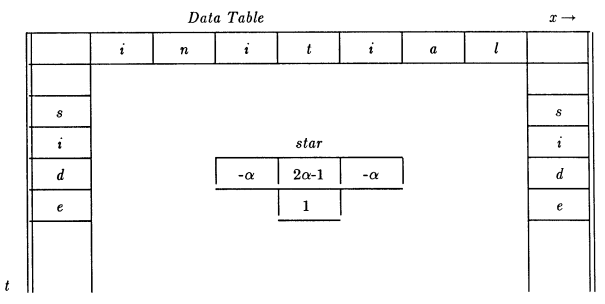
\includegraphics[width=0.95\textwidth]{new/fig2-2-1}
\caption[fig2-2-1]{一维热流方程的十字形差分系数表与数据表}
\label{fig:new/fig2-2-1}
\end{figure}
\begin{minted}{Fortran}
# Explicit heat-flow equation 
real q(12),qp(12) 
nx= 12

do ia== 1,2 { # stable and unstable cases

alpha = ia* . 3333 ; write(6, '(/"alpha=",f4.2)')alpha 

do ix= 1,6; q(ix) = 0. # Initial temperature step
do ix=7,12; q(ix) = l. 
do it= 1,6 {

write(6 , '(20f5.2)') (q(ix),ix=1,nx) 
do ix=2,nx-l
qp(ix) = q(ix) + alpha* (q(ix-1)-2. * q(ix)+q(ix+1)) 
qp(1) = qp(2);
qp(nx)=qp(nx- 1) 
do ix = 1 ,nx
q(ix) = qp(ix)
}
}
stop;end

alpha=.33
0.00 0.00 0.00 0.00 0.00 0.00 1.00 1.00 1.00 1.00 1.00 1.00 
0.00 0.00 0.00 0.00 0.00 0.33 0.67 1.00 1.00 1.00 1.00 1.00
0.00 0.00 0.00 0.00 0.11 0.33 0.67 0.89 1.00 1.00 1.00 1.00
0.00 0.00 0.00 0.04 0.15 0.37 0.63 0.85 0.96 1.00 1.00 1.00
0.00 0.00 0.01 0.06 0.19 0.38 0.62 0.81 0.94 0.99 1.00 1.00
0.00 0.00 0.02 0.09 0.21 0.40 0.60 0.79 0.91 0.99 1.00 1.00

alpha=.67
0.00 0.00 0.00 0.00 0.00 0.00 1.00 1.00 1.00 1.00 1.00 1.00 
0.00 0.00 0.00 0.00 0.00 0.67 0.33 1.00 1.00 1.00 1.00 1.00
0.00 0.00 0.00 0.00 0.44 0.00 1.00 0.56 1.00 1.00 1.00 1.00
0.00 0.00 0.00 0.30 -.15 0.96 0.04 1.15 0.70 1.00 1.00 1.00
0.00 0.00 0.20 -.20 0.89 -.39 1.39 0.11 1.20 0.80 1.00 1.00
0.13 0.13 -.20 0.79 -.69 1.65 -.65 1.69 0.21 1.20 0.87 0.87
\end{minted}
\subsection{鞋跃式方法}
采用上面给出程序的困难在于,它并非对所有可能的$\alpha$数值均有效。可以看出,当$\alpha$值过
大时(亦即$\Delta x$过小时),在数据表内部区域的解包含有不断增大的振荡。出现这种现象是因
为解的低频部分还能凑合,可是高频部分却发散。出现发散现象的准确原因将是2.8节内所
进行的某些数学分析的主题。在波长长度可与或汾相比较时,差分近似因温度之不规则
性被平滑而可望与真正的热流方程一致。在短波长时,剧烈的振荡表明差分方程可以按一种
几乎与该偏微分方程完全相反的方式来行事。短波长之所以出现偏差,是因为差分算子仅在
长波长时才等于微分算子。解的发散性是一个致命问题,因为随后出现的舍入误差往往还
会破坏低频部分。

由于假设不稳定性是因时间导数位于一个与$x$方向二阶导数所在时间$t$稍微不同的时间
$t+1/2$上所引起,于是导致所谓蛙跃式方法,这种方法将时间导数取为$t-1$与$t+1$之间的差
分:
\begin{equation}
\frac{\partial q}{\partial t}\approx \frac{q_{t+1}-q_{t-1}}{2\Delta t}
\label{eq:ex2.2.10}
\end{equation}
所得蛙跃式十宇形差分系数表形式如下:
\begin{figure}[H]
\centering
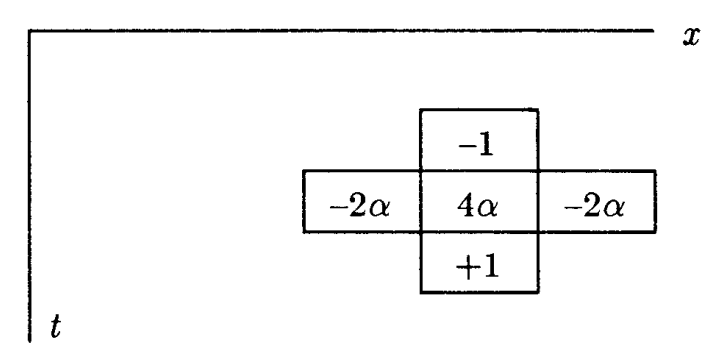
\includegraphics[width=0.5\textwidth]{new/fig-leapfrog-1}
\caption[fig-leapforg-1]{蛙跃式十宇形差分系数表形式}
\label{fig:new/fig-leapfrog-1}
\end{figure}
其实采取这种方法所得结果并不好。以后的分析将证明,对$\alpha$的所有实数值,现在的解是发
散的。将两种导数均置于相同时间位置虽然是个好主意,可是横跨许多网格点来表示一个一
阶导数,终究是个坏主意。扩展了的算子在时间方面有两个解,而不是仅只有熟知的那一个
解。数值解是两个理论解之和,不幸的是,其中一个解对$\alpha$的所有实数值是振荡増长的。

为避免所有上述这些问题(也为得到更精确的答案),我们现要转而讨论稍微更复杂一
些的求解方法,即所谓隐式方法。
\subsection{Crank-Nicolson 方法}
Crank-Nicolson法既求得准确又可解决稳定性问题。

热流方程\ref{eq:2.2.8}曾表示为
\begin{equation*}
q_{t+1}^x-q_t^x=a[q_t^{x+1}-2q_t^{x}+q_t^{x-1}]
\end{equation*}
现在,不是整个在时间$t$上表示上述右端项,而是在$t$与$t+1$上把它平均,得出
\begin{equation}
q_{t+1}^x-q_t^x=\frac{a}{2}[(q_t^{x+1}-2q_t^{x}+q_t^{x-1})+(q_{t+1}^{x+1}-2q_{t+1}^{x}+q_{t+1}^{x-1})]
\label{eq:2.2.12a}
\end{equation}
此式称为Crank-Nicolson法。令$\alpha=a/2$,则差分系数为
\begin{figure}[H]
\centering
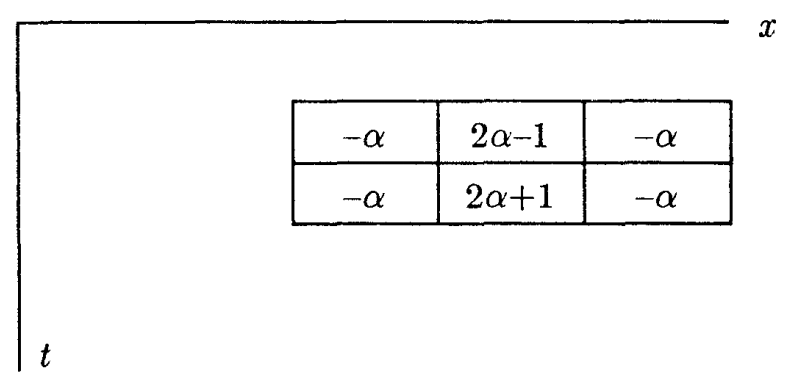
\includegraphics[width=0.5\textwidth]{new/fig-cn-1}
\caption[fig-cn-1]{蛙跃式十宇形差分系数表形式}
\label{fig:new/fig-cn-1}
\end{figure}
当把这个系数表置于数据表上时,要注意一个时间上有三个元素是未知数。为将方程也依此
处理,把式\ref{eq:ex2.2.12a}中所有的$t+1$项移至左端,而所有$t$项移至右端,得
\begin{subequations}
\begin{equation}
-\alpha q_{t+1}^{x+1}+(1+2\alpha)q_{t+1}^x-\alpha q_{t+1}^{x-1}=\alpha q_t^{x+1}+(1-2\alpha)q_t^x+\alpha q_t^{x-1}
\label{eq:2.2.13a}
\end{equation}
将所有属于$t+1$的项取为未知数,而属于$t$的项取为已知项,所以式\ref{eq:2.2.13a}的右端是已
知的,例如令其为$d_t^x$,而左端则是未知数$q_{t+1}$的一组联立方程。换言之,式\ref{eq:2.2.13a}并
未以显式的形式为我们给出每个$q_{t+1}^x$,它们是隐式地以联立方程的解给出的。如果$x$轴上只
限取五个点,则这些联立方程即为
\begin{equation}
\begin{bmatrix}
e_{lf}&-\alpha&0&0&0\\
-\alpha&1+2\alpha&-\alpha&0&0\\
0&-\alpha&1+2\alpha&-\alpha&0\\
0&0&0&-\alpha&e_{rt} 
\end{bmatrix} 
\begin{bmatrix}
q_{t+1}^1\\q_{t+1}^2\\q_{t+1}^3\\
q_{t+1}^4\\q_{t+1}^5
\end{bmatrix}
=
\begin{bmatrix}
d_t^1\\d_t^2\\d_t^3\\d_t^4\\d_t^5
\end{bmatrix} 
\label{eq:2.2.13b}
\end{equation}
\end{subequations}
值$e_{lf}$和$e_{rt}$是可调节的,并且必须按旁侧边界条件来调节。值得注意的重要事情是,该矩阵
是三对角线矩阵,即,除三个中心对角线上的元素外,矩阵\ref{eq:2.2.13b}中所有其他元素均
为零。能够快速地得出这一类联立方程的解,其计算时间大约仅二倍于式\ref{eq:2.2.9}给出的显
式方法。事实上,由于式\ref{eq:2.2.13a}的精度高于式\ref{eq:2.2.9},允许利用非常大的时间步长$\Delta t$,
结果这种隐式方法证明是种节省时间的方法。下面给出一个可以说明即使是对很大$\Delta t$,
该方法也具有稳定性的程序。

\begin{minted}{Fortran}
# Implicit heat-flow equatioil 
real q(12),d(12),e(12),f(12)

nx= 12;a=8.; write(6,'(/"a= ",f4.2)')a; alpha= .5*a 
do ix= 1,6; q(ix)= 0. # Initial temperature step
do ix=7,12; q(ix)= 1. 
do it== 1,4 {
write(6,'(20f5.2)') (q(ix),ix= 1,nx) 
d(l)=0.; d(nx)= 0. 
do ix=2,nx-l
d(ix)=q(ix) + alpha*(q(ix-l)-2.*q(ix) + q(ix+ 1)) 
call rtris(nx,alpha,-alpha,( l. + 2.*alpha),-alpha,alpha,d,q,e,f)
}
stop; end 
# real tridiagonal equation solver

subroutine rtris(n,endl,a,b,c,endr,d,q,e,f) 
real q(n),d(n),f(n),e(n)
e(1) =-a/endl; f(1) = d(1)/endl
do i = 2,n-l {
den = b + c*e(i-1); e(i) = -a/den;  f(i)= (d(i)-c*f(i-1))/den } 
q(n) = (d(n)-c*f(n-1))/(endr+ c*e(n-1))
do i = n-1,1,-1
q(i) = e(i)*q(i + 1) + f(i) 
return; end

a = 8.00
0.00 0.00 0.00 0.00 0.00 0.00 1.00 1.00 1.00 1.00 1.00 1.00
0.17 0.17 0.21 0.30 0.47 0.76 0.24 0.53 0.70 0.79 0.83 0.83
0.40 0.40 0.42 0.43 0.40 0.24 0.76 0.60 0.57 0.58 0.60 0.60 
0.44 0.44 0.44 0.44 0.48 0.68 0.32 0.52 0.56 0.56 0.56 0.56
\end{minted}
计算中采用了求解三对角线联立方程的子程序,下一节将对该子程序加以解释。
\subsection{求解三对角线联立方程}
全世界有很多计算力量都忙于应付求解三对角线联立方程。为参考和完整起见,本节内
容也将涉及算法。

设将联立方程写成某种差分方程组
\begin{equation}
a_iq_{i+1}+b_iq_i+c_iq_{i-1}=d_i
\label{eq.ex2.2.14}
\end{equation}
按照某种方程
\begin{equation}
q_i=e_iq_{i+1}+f_i
\label{eq.ex2.2.15}
\end{equation}
引入两个新未知数$e_i$与$f_i$,用经过时移的下标写出式\ref{eq.ex2.2.15}
\begin{equation}
q_{i-1}=e_{i-1}q_{i}+f_{i-1}
\label{eq.ex2.2.16}
\end{equation}
将\ref{eq.ex2.2.16}代入\ref{eq.ex2.2.14},得
\begin{equation}
a_iq_{i+1}+b_iq_i+c_i(e_{i-1}q_{i}+f_{i-1})=d_i
\label{eq.ex2.2.17}
\end{equation}
现将式\ref{eq.ex2.2.17}重新排列,使之类似于\ref{eq.ex2.2.15}
\begin{equation}
q_i=\frac{-a_i}{b_i+c_ie_{i-1}}q_{i+1}+\frac{d_i-c_if_{i-1}}{b_i+c_ie_{i-1}} 
\label{eq.ex2.2.18}
\end{equation}
将式\ref{eq.ex2.2.18}与式\ref{eq.ex2.2.15}比较即可看出,新的未知数$e_i$与$f_i$的递归公式为
\begin{subequations}
\begin{equation}
e_i=\frac{-a_i}{b_i+c_ie_{i-1}}
\label{eq:ex2.2.19a}
\end{equation}
\begin{equation}
f_i=\frac{d_i-c_if_{i-1}}{b_i+c_ie_{i-1}} 
\label{eq:ex2.2.19b}
\end{equation}
\label{eq:ex2.2.19}
\end{subequations}
首先必须给出左侧边界的某种边界条件,这种条件也许会涉及一个点或两个点。最一般性的
可能的边缘终端条件是一种在$i=0$时类似于方程\ref{eq.ex2.2.15}
的线性关系,即$q_0=e_0q_1+f_0$。
因此边界条件必须给出$e_0$与$f_0$,利用$e_0$以及所有的$a_i$,$b_i$,$c_i$,我们就可采用式\ref{eq:ex2.2.19a}
计算出所有的$e_i$。
在右端的边界,我们需要另一种边界条件,最一般性的两点式边界条件为
\begin{equation}
c_{n-1}q_{n-1}+e_{rt}q_n=d_n
\label{eq:ex2.2.20}
\end{equation}
作为特殊情形,此式包括了零值边界条件与零斜率边界条件。式\ref{eq:ex2.2.20}可与式\ref{eq.ex2.2.16}在其端点上时的情形相比
\begin{equation}
q_{n-1}=e_{n-1}q_n+f_{n-1}
\label{eq:ex2.2.21}
\end{equation}
$q_n$与$q_{n-1}$均为未知数,不过,式\ref{eq:ex2.2.20}与\ref{eq:ex2.2.21}是两个方程,所以求解很容易。最
后一步是取$q_n$的值,并在式\ref{eq.ex2.2.16}中利用它计算出$q_{n-1}$、$q_{n-2}$、$q_{n-3}$等等。

如果你希望尽可能充分发挥你的讨算机潜力,则应注意有关这种算法的若干事实:
\begin{enumerate}
\item $e_i$值的计算通过$a_i$、$b_i$、$c_i$而与介质有关,但与解$q_i$无关(即使是通过$d_i$),这意昧着它有
可能节省计算时间,而可重复利用$e_i$。
\item 许多计算机都是除法比乘法慢得多,因此,可以将式\ref{eq:ex2.2.19a}、\ref{eq:ex2.2.19b}中的除数之倒数一次求出来,而且或许可存储起来以备重复使用。
\end{enumerate}
\subsection{导数$\partial^3/\partial x^2\partial z$}
45°绕射方程不同于15°绕射方程之处在于前者包括有导数$\partial^3/\partial x^2\partial z$。幸运的是,这种导
数可适应六点差分系数表
\begin{figure}[H]
\centering
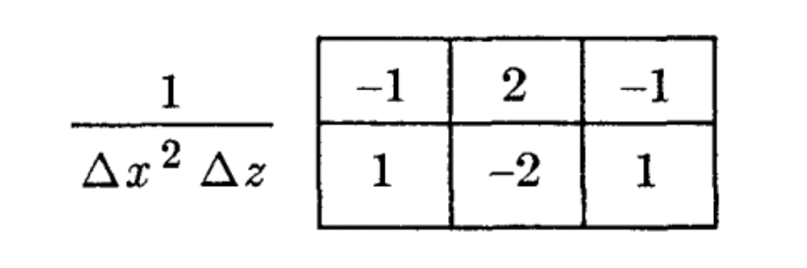
\includegraphics[width=0.5\textwidth]{new/fig-2-2-22}
\caption[fig-2-2-22]{六点差分系数表形式}
\label{fig:new/fig-2-2-22}
\end{figure}
所以,除了改变系数表上的六个系数之外,它并不会对计算效率造成什么影响。
\subsection{高维方程的困难}
迄今,为获得节省时间而又精确可靠的求解偏微分方程之差分方法,我们还未遇到麻
烦,隐式方法已可满足所有的需要。
可是,在高于一维的空间域,隐式方法的运算时间就高
得使人不敢问津了。我们将以$\partial^2/\partial x^2$推广为$\partial^2/\partial x^2+\partial^2/\partial y^2$的普通问题为例来讨论一下其
理由何在。最简单的情形就是热流方程,由Crank-Nicolson方法给出式\ref{eq:2.2.13a}。引入缩
写$\delta_{xx}q=q^{x+1}-2q^x+q^{x-1}$,式\ref{eq:2.2.13a}变为
\begin{equation}
(1-\alpha\delta_{xx})Q_{t+1}=(1+\alpha\delta_{xx})Q_{t}
\label{eq:ex2.2.23}
\end{equation}
左端括内的表达式代表一个三对角线矩阵,关键之处在于4求解未知数$Q_{t+1}$向量的三对角
线联立方稆。值把庆幸的是有一种获得该解的特殊算法,其计算时间仅随矩阵之大小而线性
增加。现在就从$x$的一维物理空间转而讨论二维空间$(x,y)$,
令$\alpha$表示式\ref{eq:ex2.2.23}中的
数值常数,于是按时间步进的方程为
\begin{equation}
[1-\alpha(\delta_{xx}+\delta_{yy})]Q_{t+1}=[1+\alpha(\delta_{xx}+\delta_{yy})]Q_t
\label{eq:ex2.2.24}
\end{equation}
未知数$Q_{t+1}$是$x$与$y$的二维函数,可用一个矩阵表示。其次,我们将解释一下左端括号内的
表达式,结果证明它是一个四维矩阵!

\section{单频波的程序}
我们将按他的启示行事。你的第一个问题与图\ref{lst:code2.3.1}所示之计算机程序有关。照实际情形来说,它将产生通过某一能量的波动传播的活动电影
(三维矩阵形式)。从编辑到计算直至最终看见循环影片的整个过程,约为一分钟(当你是计算机仅有的用户的时候)。
\subsection{循环影片程序之分析}
要使循环影片对观众有意义,电影的主题必须是周期性的,从而必须安排得使最后的
面很自然地与第一个画面衔接起来。在图\ref{lst:code2.3.1}所示程序形成的电影中,有一个参量
lambda,它控制着从顶部照亮屏幕之波动脉冲的基本重复率。当一个子波往下传播了四分
之一画面的路程时,另一个子波就应送进去。这种过程由下列一行程序来规定
\begin{equation*}
lambda=nz*dz/4=\frac{N_z\Delta_z}{4}
\end{equation*}
各脉冲均由频率为$n\omega$、即$\Delta \omega$、$2\Delta\omega\ldots\ldots$,$n\omega\Delta\omega$等之正弦波叠加而形成,最低频率$d\omega=\Delta\omega$
具有与lambda呈反比的波长。因此规定
\begin{equation*}
d\omega=v\times\pi^2/lambda=\frac{2\pi v}{\lambda}
\end{equation*}
最后,循环影片的延续时间必须等于最低频正弦波的周期
\begin{equation*}
N_t\Delta t=\frac{2\pi}{\Delta \omega}
\end{equation*}
最后这个方程定义了关于扫描线的时间间隔
\begin{equation*}
dt=\pi^2/(nt\times d\omega)
\end{equation*}
该程序所求解的偏微分方程为
\begin{equation}
\frac{\partial P}{\partial z}=\frac{i\omega}{v(x,z)}P+\frac{v}{-i\omega^2}\frac{\partial^2 P}{\partial x^2}
\label{eq:ex2.3.1}
\end{equation}
对于每个步长$\Delta z$,完成两步计算,第一步是解
\begin{equation}
\frac{\partial Q}{\partial z}=\frac{v}{-i\omega^2}\frac{\partial^2 Q}{\partial x^2}
\label{eq:ex2.3.2}
\end{equation}
利用Crank-Nicolson差分方法,此式变为
\begin{equation*}
\frac{q_{z+1}^x-q_z^x}{\Delta z}=-\frac{v}{i\omega^2}[\frac{q_z^{x+1}-2q_z^x+q_z^{x-1}}{2\Delta x^2}+
\frac{q_z^{x+1}-2q_{z+1}^x+q_{z+1}^{x-1}}{2\Delta x^2}]
\end{equation*}
将所有常数减缩成一个常数,并定义:
\begin{equation}
\alpha=\frac{v\Delta z}{-i\omega^4\Delta x^2}
\label{eq:ex2.3.3}
\end{equation}
得到
\begin{equation*}
q_{z+1}^x-q_z^x=\alpha[q_z^{x+1}-2q_z^x+q_z^{x-1}+q_z^{x+1}-2q_{z+1}^x+q_{z+1}^{x-1}]
\end{equation*}
将各未知数置于左端,则
\begin{equation}
-\alpha q_{z+1}^{x+1}+(1+2\alpha)q_{z+1}^x-\alpha q_{z+1}^{x-1}=\alpha q_z^{x+1}+(1-2\alpha)q_z^x+
\alpha q_z^{x-1}
\label{eq:ex2.3.4}
\end{equation}
第二步是解下述方程
\begin{equation}
\frac{\partial Q}{\partial z}=\frac{i\omega}{v}Q
\label{eq:ex2.3.5}
\end{equation}
其解析解为
\begin{equation}
Q(z+\Delta z)=Q(z)e^{i\frac{\omega}{v}\Delta z}
\label{eq:ex2.3.6}
\end{equation}
图\ref{lst:code2.3.1}中的程序严格按\ref{eq:ex2.3.3}、\ref{eq:ex2.3.4}与\ref{eq:ex2.3.6}各式而编制。
\begin{listing}[H]
  \caption{产生单频波之和的电影的计算机程序}
  \inputminted{Fortran}{timespace/code2-3-1.f90}
  \label{lst:code2.3.1}
\end{listing}
\subsection{相移}
为作出波动脉冲,须将若干频率成分相加起来。在这个程序中,只利用了两个频率
$nw=2$。如果你试图只用一个频率$nw =1$
,则有些事情就变得不太清晰了。在侧边界上反射
回来的波看起来更像是驻波(参考练习2)。如果你试图采用更多频率,程序就将比较长了,
但是你会更喜欢那画面,因为脉冲之间的平静区会比较长而平静一些。各种频率成分可采用
不同的加权。
%\begin{minted}{Fortran}
%# submit
%nx = 13
%\label{prog:2.3.1}
%\end{minted}

% \begin{figure}[H]
% \centering
% 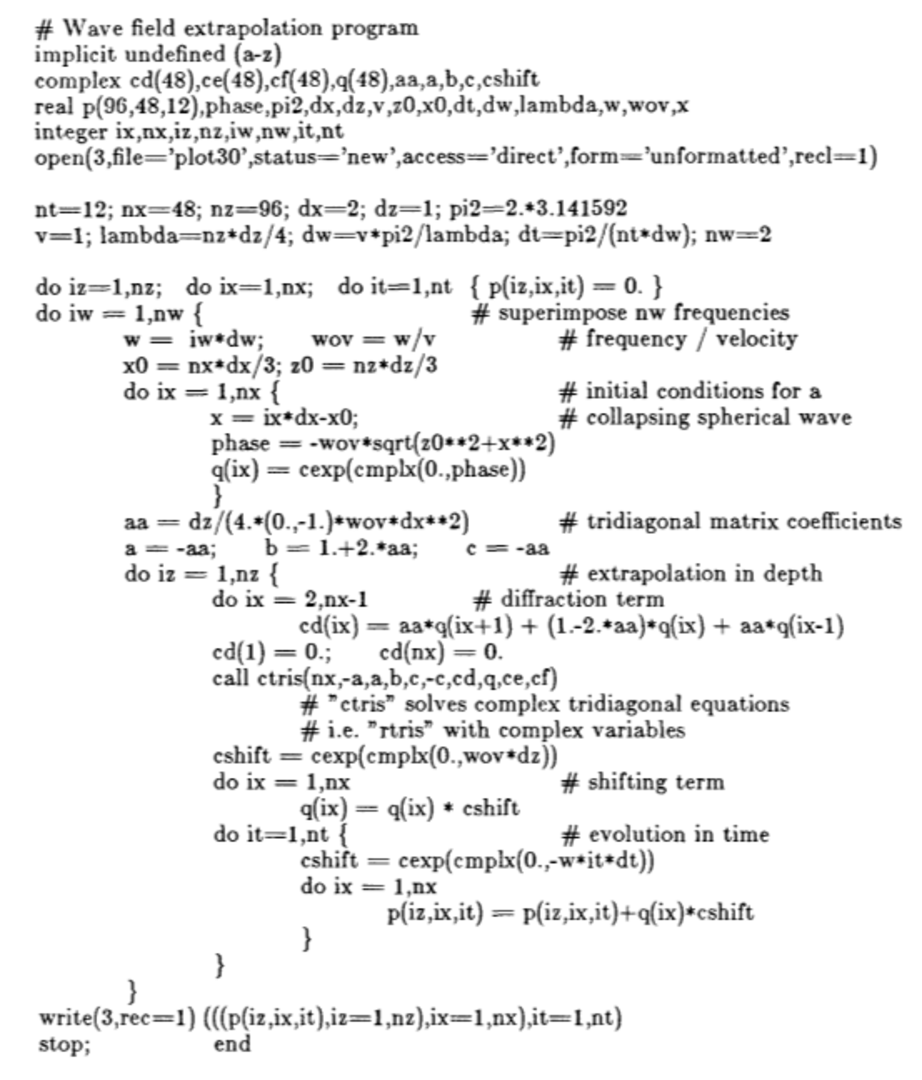
\includegraphics[width=0.85\textwidth]{new/fig-2-3-1}
% \caption[code2-3-1]{产生单频波之和的电影的计算机程序}
% \label{fig:new/fig-2-3-1}
% \end{figure}
理论预言,经过一焦点的二维波动将经受90°的相移。你应能注意到,一个对称波形入
射在焦点上,但是却形成了一个反对称的波形。(在图\ref{fig:2.3.6}中可以很好地看出这点,但在电影
中比较清楚)。在地震偏移方法中,波是正好到达焦点而不是通过它,所以二维情形的偏移脉
冲响应有45°相移。尽管现实世界是三维的,对于推测是由柱面而非球面反射面引起聚焦之
处的地震测线,适宜于进行偏移的却是二维响应。

\subsection{横向速度变化}
横向速度变化$v=v(x)$尚未包括在程序之中,不过把它加进去并不困难。它从两个地
方进入程序,第一是进入式\ref{eq:ex2.3.6},如果$k_x$是足够小以致可忽略不计的数据,则式
\ref{eq:ex2.3.6}就是仅有的需要该项速度之处。第二是进入三对角线系数。光学上的所谓薄透镜
近似看来好像仅只相当于包括式\ref{eq:ex2.3.6}这一部分。

\subsection{侧边界分析}
在地球物理学中,我们通常都希望别同侧边界问题沾边。要考虑侧边界问题的唯一实际
原因是我们的勘测或者我们的处理活动有必要对其范围加以限制。既然侧边界是不可避免
的,那我们就必须想办法对付它。\ref{lst:code2.3.1}内的程序包括有零斜率边界条件,取
\begin{equation*}
d(1)=0.; d(nx)=0.
\end{equation*}
并在调用子程序“ctris”时取
\begin{equation*}
endl= -a ; endr = -c
\end{equation*}
即可形成此类边界条件。得到零值侧边界条件的快速方法是取
\begin{equation*}
endl = endr = 10^{30}\approx\infty
\end{equation*}
上述处理办法稍微有点浪费计算机内存,因为端点的零值要存储起来,而零斜率则可明
显看成是有两个相同的记录道,Dave
Hale所编制的程序可避免这种浪费,该程序给出如下:
\begin{minted}{Fortran}
qO = bl * q ( 1 ) ; qnxpl=br * q ( nx )

cd ( 1 ) = aa * q ( 2 ) + (1.-2. * aa ) * q ( 1 ) +aa * qO
cd ( nx ) =aa * q ( nx-1 ) + ( 1.-2. * aa ) * q ( nx )+aa * qnxpl

endl=c * bl + b;
endr=a * br + b

call ctris (nx, endl, a, b, c, endr, cd, q, ce, cf)
\end{minted}
注意,对于零值边界应$bl=br=0$,对于零斜率边界则应$bl=br=
l$。令bl与br为复数,则可得到\ref{sec:4.4}节中将导出的吸收边界条件。

\subsection{关于循环影片程序的若干变种}
通过以下的一些练习来记录你的进步,在准备期终考试时,这将是有帮助的。而且此后
若干年你都能重温你的记忆。

准备一本活页笔记簿,把所有图件和程序纸裁成长11宽$8\frac{1}{2}$大小,并穿三个孔。若需要
进行代数分析,那就在另一张同样大小的纸上作,别把重要一点的分析写在碎纸片上。这份
材料同你的课堂笔记一起保留,或者作为一本实验笔记簿保存。始终别忘填上日期。

对这些练习的每一个题,均须送交一份程序和第一个画面的图。

练习1试说明如何改变程序,使之得出一个右侧偏离垂直线呈15°角度向下传播的初始
平面波。

练习2已知计算域为$0<x\leq x_{max}$和$0<z\leq z_{max}$,你将如何更改$z=0$处的初始条件,使
之可模拟一在$(x,z) =(x_{max}/3,-z_{max}/2)$处的点源?

练习3试修改程序,使得可用零偉侧边界来代替零斜率边界。

练习4试对衰减球面波应用45°项$\partial _{xxz}$。利用零斜率边界。将你所得结果同用图\ref{lst:code2.3.1}的
程序所得结果进行比较。在理论焦点位置上作一记号$X$。

练习5对程序进行一些改变,使之包括一个薄透镜项,通过恒定慢度梯度所产生的画
面时该透镜项具有40\%的横向速度变化.识别出程序中为横向速度变化所影响的其他部分。
你无需去进行其他这些改变。试问为何预计这些变化会很小?

练习6试利用位于$(x,z)=(x_{max}/2,0)$的一个点震源来检验程序,请观察并描
绘出各种计算产生的假象。这类震源富含很高空间频率,在这种情况下,差分方程无法模拟
其相应的微分方程。

练习7 \ref{sec:4.4}节将阐述如何在侧边界上使能量被吸收。试按此要求对程序作必要的改 变。

练习8采用以后在\ref{sec:4.3}
节述及的方法能够改善$x$方向的导数之精度。主要之点是,不用
主对角线元素为$(-1,2,-1)$的三对角线矩阵$\mathbf{T}$来代表$k_x^2\Delta x^2$,而是用$\mathbf{T}/(\mathbf{I}-\mathbf{T}/6)$。因
遍乘以该分母而须修改原来的外推分析方法。试对45°衰减波的程序进行必要的改变。
\begin{figure}[H]
\centering
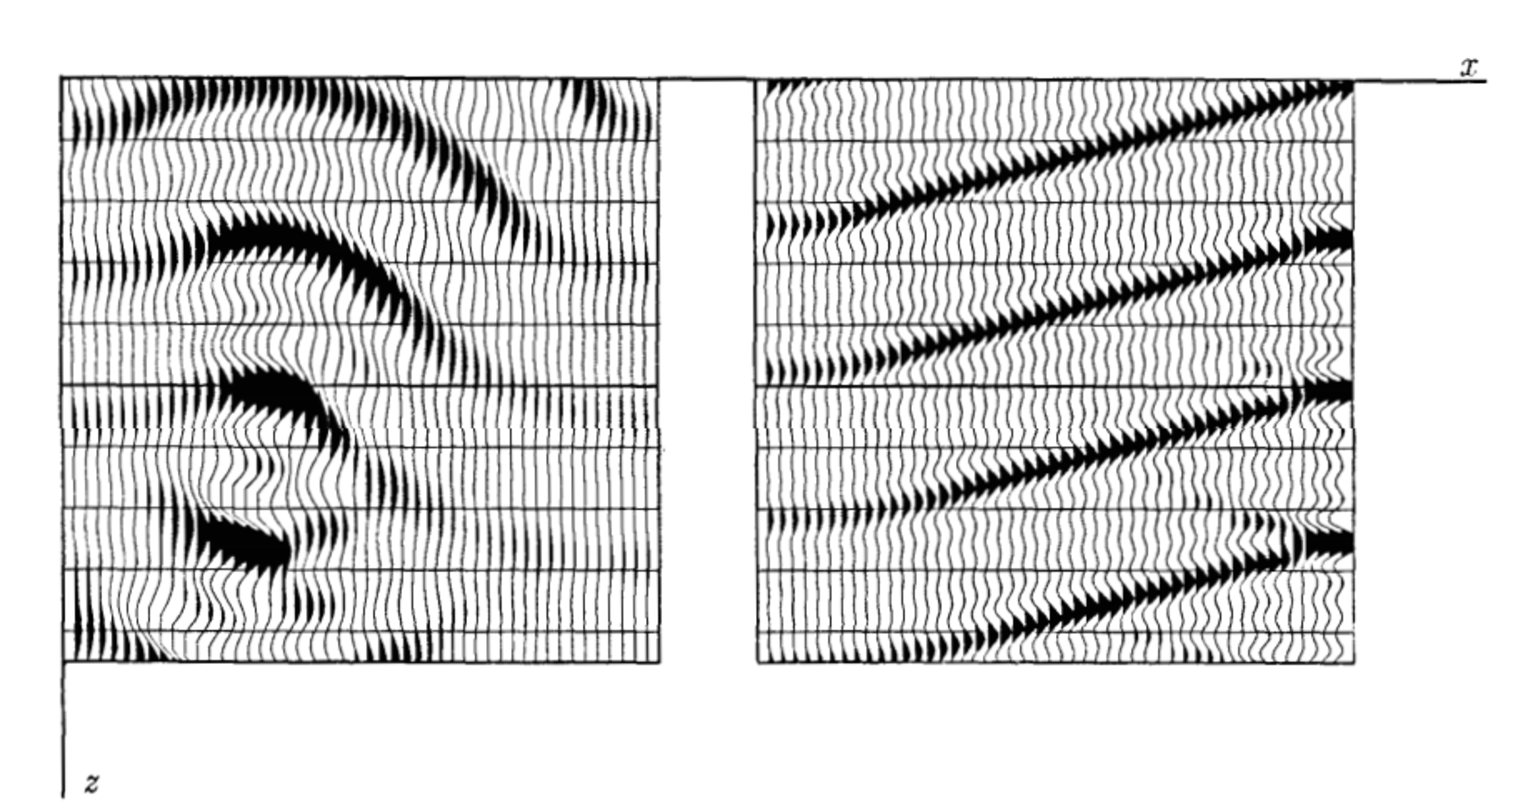
\includegraphics[width=0.85\textwidth]{new/fig-2-3-2}
\caption[2-3-2]{左:由图\ref{lst:code2.3.1}所产生的第一个电影画面;右:练习1的解}
\label{fig:new/fig-2-3-2}
\end{figure}

\begin{figure}[H]
\centering
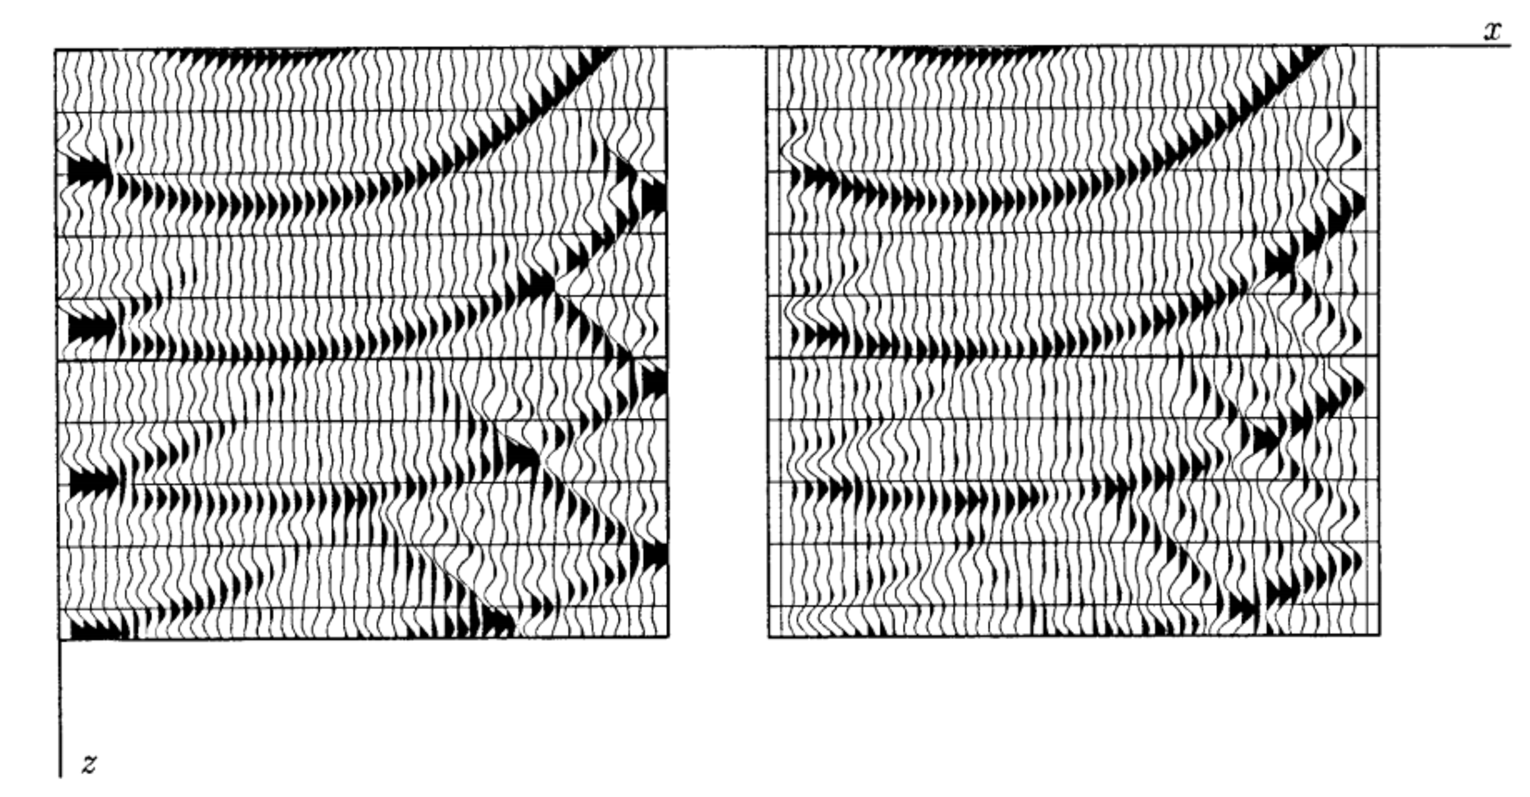
\includegraphics[width=0.85\textwidth]{new/fig-2-3-3}
\caption[2-3-3]{左:练习2,扩展的球面波;右:练习3,零值侧边界}
\label{fig:new/fig-2-3-3}
\end{figure}

\begin{figure}[H]
\centering
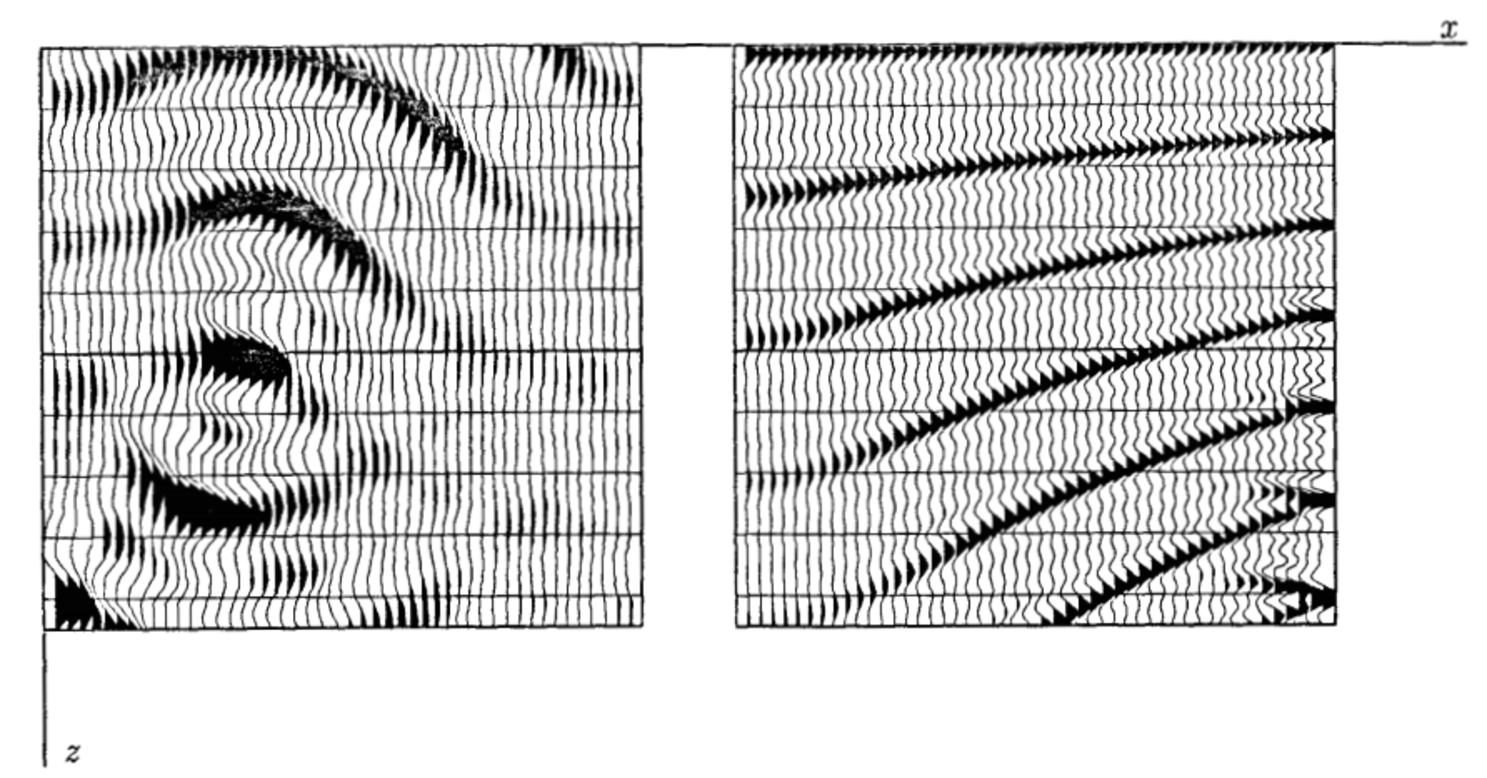
\includegraphics[width=0.85\textwidth]{new/fig-2-3-4}
\caption[2-3-4]{左:练习4,45°项;右:练习5,横向速度变化}
\label{fig:new/fig-2-3-4}
\end{figure}

\begin{figure}[H]
\centering
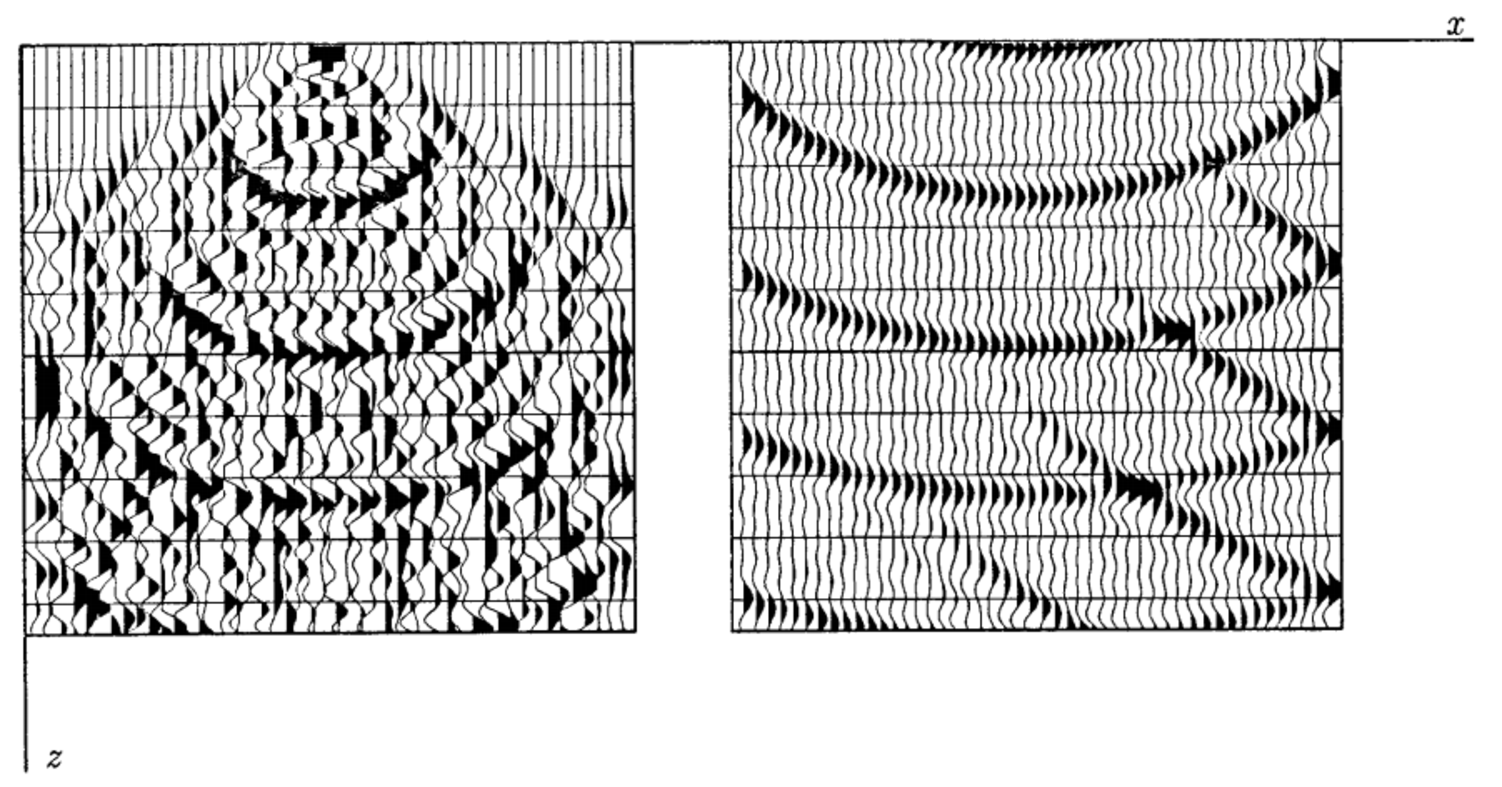
\includegraphics[width=0.85\textwidth]{new/fig-2-3-5}
\caption[2-3-5]{左:练习6,与点震源有关的计算假象;右:练习7,吸收边界}
\label{fig:new/fig-2-3-5}
\end{figure}

\begin{figure}[H]
\centering
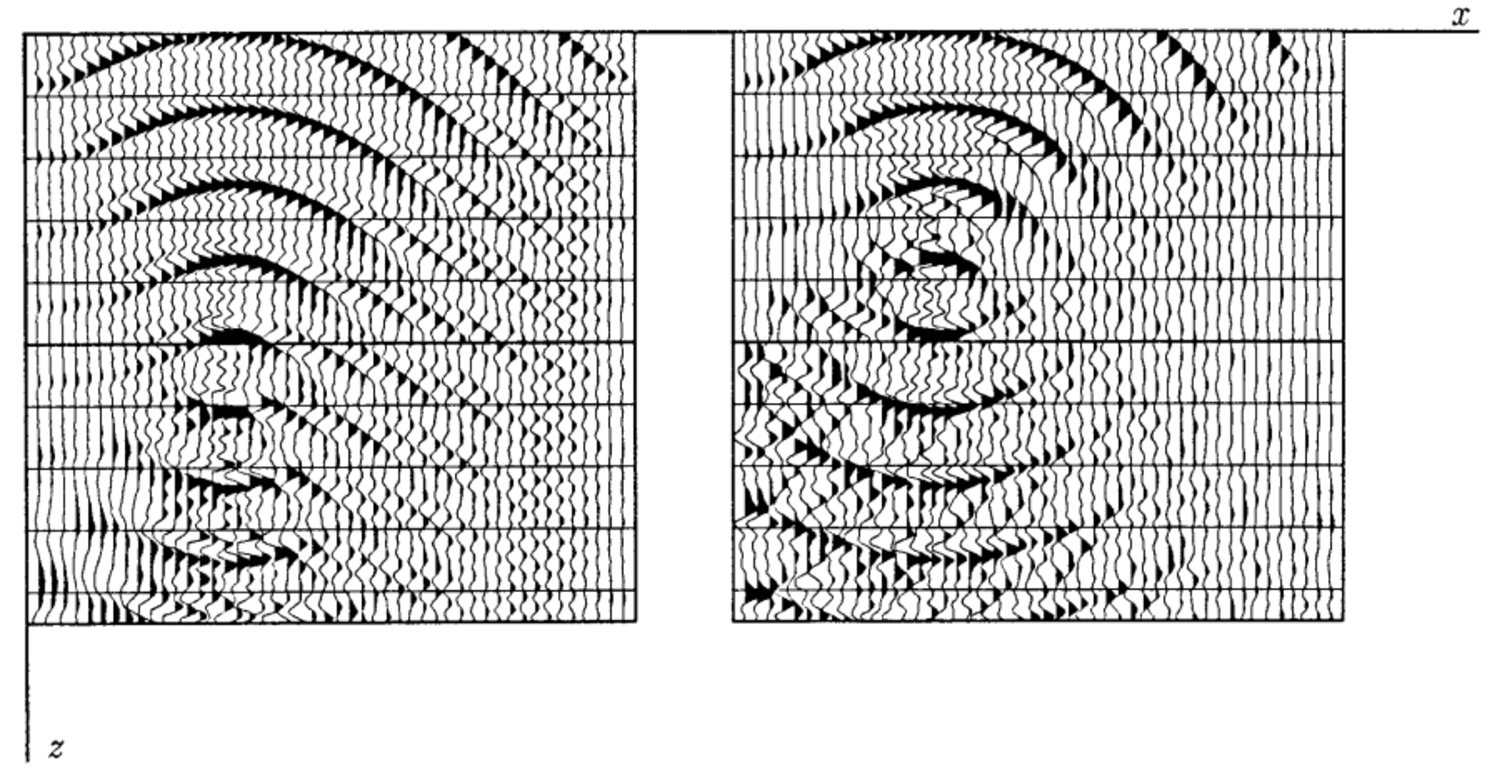
\includegraphics[width=0.85\textwidth]{new/fig-2-3-6}
\caption[2-3-6]{左:练习8,未采用1/6技巧;右:米用1/6技巧}
\label{fig:new/fig-2-3-6}
\end{figure}

\subsection{$(\omega,x,z)$域内的偏移程序(Kjartansson,Jacobs)}
偏移程序类似于循环影片程序,不过有一些差别。循环影片要作四重嵌套循环,它对时
间$t$的许多值产生结果。偏移则只要求在$t=0$时的值,所以省掉一重循环,这意味着用同等
数量的计算机时间可计算出更大的空间体积。可惜,失掉一次循环也就意味着失掉了以电
影形式显示的可能。采用$\omega$频率域偏移时,看来要考虑的唯一有意义的事就是输入与输出
了。

同循环电影不一样,这种过程的输入恐怕将会是野外数据了,所以不会存在频率域的解
析表达式。由于将在时间域内输入,因而必须进行Fourier变换。\ref{fig:new/2.3.7}所示程序的开始部
分定义一呰模拟野处数据的脉冲,这些全是宽脉冲,应将其偏移至近似半圆上。因为差分算子对微分算子的偏差会造成干扰混乱,所以就没利用准确的脉冲。

然后,该程序以Fourier变换方法把人工合成数据从时间域变换至频率域。

接着将每一频率成分向下延拓,这是沿深度$z$和沿频率$\omega$进行的一种循环。这两个循环
中随便那一个都可以是内循环,如何选择决定于计算机效率。

同循环影片程序要求用下行波方程不同,偏移是要求用上行波方程,所以要改变式
\ref{eq:ex2.3.1}中$z$轴的符号,这种改变影响到aa的符号和cshift的钼位符号。

和循环影片不同的另一个差别是,现在的输入有时间轴,而输出则仍为深度轴。习惯上为
方便起见,要重新组织计算过程,不是按深度而是按旅行时间“深度”显示,使输入与输出
的垂直轴相同。利用$\tau=z/v$与$d\tau/dz=1/v$的等价关系,由微分法则得出
\begin{equation}
\frac{\partial}{\partial z}=\frac{\partial\tau}{\partial z}\frac{\partial}{\partial \tau}=\frac{1}{v}\frac{\partial}{\partial \tau}
\label{eq:2.3.7}
\end{equation}
代入式(1)中,得
\begin{equation}
\frac{\partial P}{\partial \tau}= -i\omega P-\frac{v^2}{-i\omega 2}\frac{\partial^2 P}{\partial x^2}
\label{eq:2.3.8}
\end{equation}

在该程序中,时间采样间隔心=洫及旅行时间“深度”采样间隔$dtau=\Delta\tau$均取为1,因
此极大频率即是Nyquist频率。应注章,沿频率的循环只涉及正值频率轴。负值频率仅只用来保持时间函数为实函数,只需取实部就能很容易地做到这点。

% \begin{code}
% \begin{minted}[frame=single]{py}
% def my_func(x):
%     print x
% \end{minted}
% %\caption{My func}
% \label{lst:my_func}
% \end{code}
\begin{listing}[H]
  \caption{$(\omega,x,z)$域内的偏移程序}
  \inputminted{Fortran}{timespace/code2-3-7.f90}
  \label{lst:code2.3.7}
\end{listing}
偏移程序运算结果的输出如图\ref{fig:omx/kjartjac}所示。你看见的主要是半圆近似。在较晚的时间上
还有一些计算假象,可能是频率域假频影响所致。输入脉冲具有相当宽的倾斜条带状外形,
所以该图预告了以后将要加以证明的一件事实,即,半圆近似实际上是一个经过原点的椭
圆。

注意,原始脉冲的波形原是一种对称的时间函数,而现在半圆上的波形表现为既非对
称又非反对称,它是一种45°相移脉冲的波形,三维空间内一个点源所产生的波将具有90°相
移,由三维空间内一个二维爆炸反射面产生的波则应具有45°相移。

\begin{figure}[H]
\centering
\includegraphics[width=0.5\textwidth]{omx/kjartjac}
\caption[kjartjac]{程序\ref{lst:code2.3.7}的输出:半圆近似}
\label{fig:omx/kjartjac}
\end{figure}

\section{分裂法与全分离法}
\label{sec:2.4}
通常同时起作用的两个过程A与B也许是或者
也许不是相互联系的。它们相互独立的这种情形, 称作全分离(full separation)
。在这种情形下,就概念和就计算而言,想像A过程在B过程开始之
前正趋近于结束,这往往是很有用的。在两种过程
彼此有相互联系的场合,有可能是允许A短暂起作
用,然后转换为B起作用,并如此交替作用下去,
这种交替起作用的办法称作分裂法(splitting)。

\subsection{热流方程}
\label{sec:2.4.1}
绕射方程或偏移方程可称作“波阵面恢复”方程,它把初始条件或透镜项可能引起的波阵面的任
何横向突变一起加以平滑恢复原状。
15°偏移方程具有有与热流方程相同的数学形式。不过热
流方程全是实数,而且它的物理性态更容易理解,这点值得多说两句:(l)x方向的热流
$H_x$等于温度的负梯度$-\partial T/\partial x$如乘以热传导率$\sigma$。(2)温度降低$-\partial T/\partial t$是同热流发散量$\partial H_x/\partial x$
除以热容量c成比例。将上述二者结合起来并由一维情形推广至二维情形,取$\sigma$为常数及
$c=l$,得出方程:
\begin{equation}
\frac{\partial T}{\partial t}=\sigma[\frac{\partial^2}{\partial x^2}+\frac{\partial^2}{\partial y^2}]T
\label{eq:ex2.4.1}
\end{equation}

\subsection{分裂法}
\label{sec:2.4.2}
应用于热流方程数值解法的分裂法是用两个微分方程代替热流方程,按交替的时间步长
应用其中每个方程
\begin{subequations}
\begin{equation}
\frac{\partial T}{\partial t}=2\sigma\frac{\partial^2 T}{\partial x^2} \quad (all\quad y)
\label{eq:ex2.4.2a}
\end{equation}
\begin{equation}
\frac{\partial T}{\partial t}=2\sigma\frac{\partial^2 T}{\partial y^2} \quad (all\quad x)
\label{eq:ex2.4.2b}
\end{equation}
\label{eq:ex2.4.2}
\end{subequations}

式\ref{eq:ex2.4.2a}中,对于x方向的热流其热传导率$\sigma$业已增大两倍,而对$y$方向的热流则已取$\sigma$
为零;在式\ref{eq:ex2.4.2b}中,则情形反之。在时间的奇数时刻,热量按式\ref{eq:ex2.4.2a}的关系流
动;在时间的偶数时刻则按式\ref{eq:ex2.4.2b}的关系流动。这种轮流交替采用式\ref{eq:ex2.4.2a}与
\ref{eq:ex2.4.2b}所得的解在数学上可证明是收敛于式\ref{eq:ex2.4.1}的解,其误差为$\Delta t$数量级,因此
汾趋于零时,误差亦趋于零。高维隐式方法的不可行性是促使采用分离法的原因(参阅\ref{sec:2.2}
节结尾部分)。

\subsection{全分离法}
\label{sec:2.4.3}
最终可证明分裂法比可能想像的要精确得多,在许多情形下不存在精度损失。此外,可
认为这种方法是一种极限情形。试考虑一下处理方程\ref{eq:ex2.4.2a}与\ref{eq:ex2.4.2b}的基本方
法,在这种处理中,不是按交错的时间步长在它们之间轮流进行前向与后向计算,而是通过
所有时间步长将方程\ref{eq:ex2.4.2a}计算到底,然后再将这种中间计算结果作为方程\ref{eq:ex2.4.2b}
的初始条件,经过所有时间步长将式\ref{eq:ex2.4.2b}计算到底,得出最终结果。也许会令人惊
奇,这种经过基本改变的方法可以产生方程\ref{eq:ex2.4.1}的正确解。但是,只在$\sigma$是$x$与$y$的一个恒定
函数时,才能如此。对于脉冲型初始扰动的情形,该种过程如图\ref{fig:txz/temperature}所示。在用这种基本
方法获得正确的解时,就把像\ref{eq:ex2.4.1}那样的一种微分方程说成是可全分离的。全分离法
在$\sigma$为常数时才有效,这点不应使人感到太奇怪,因为这时才能够应用Fourier变换,从而
二维解$exp[-\sigma(k_x^2+k_y^2)t]$等于一维解$exp(-\sigma k_x^2t)$与$exp(-\sigma k_y^2t)$之乘积。可以证明
并且以后将会指出,可应用全分离法的条件就是$\sigma \partial^2/\partial x^2$应能与$\sigma \partial^2/\partial y^2$交换。从技术上说,
还存在一个边界条件的要求,不过当扰动在到达边界之前即衰减掉时,这点不会造成什么困
难。
\begin{figure}[H]
\centering
\includegraphics[width=0.95\textwidth]{txz/temperature}
\caption[temperature]{$(x,y)$平面内的温度分布。开始时为delta函数形状(左)。允许沿$x$方向但不沿$y$方向流动之后,热
量分希位于一片状区域内(中)。最后,允许热量沿$y$方向但不沿$x$方向流动,
得出同样的对称高斯分布的结果,其最终形状犹如热量同时沿$x$方向与$y$方向
流动,(右)}
\label{fig:txz/temperature}
\end{figure}


令人奇怪,在许多有关数值解的教科书中对全分离性没怎么介绍,这也许是由于不论是用
分裂法还是用全分离法求解,其加法与乘法的总次数是相同之故。但是,作为一个实际问
题,求解大数据量问题的计算时间并非简单随乘法次数而增高。当数据库不能整个输入于随
机存取器时(这差不多就是大数据量问题的定义),则分裂法的每一步骤都要求将数据库
加以转置。例如,从$(x,y)$的存储顺序转置成$(y,x)$的存储顺序。转置所要求的就不
是乘法,可是在许多情况下,转置所需时间却远超出整个计算所耗费的时间。所以,若进行
转置是不能避免时,至少应使它减少至实际允许的极小限度。有一些情况使得非在分裂法与
全分离法之间采取折中办法不可。例如,如果$\sigma$是$x$与$y$的一个缓慢变化的函数
时,就得如此,这时会发现,虽然$\sigma \partial^2/\partial x^2$并非严格可与
$\sigma \partial^2/\partial y^2$交换,可是却足够接近,因而在对数据进行转置
和转换至式\ref{eq:ex2.4.2b}之前,能够继续用式\ref{eq:ex2.4.2a}进行若干时间
步长的计算。以下要考虑的波场外推方程就是类似于这样一种但更具有地球物理意义的情况。第一个认识
到分裂法与全分离法概念在地震学中的意义是Brown(1983)。

\subsection{应用于横向速度变化情形}
\label{sec:2.4.4}
有一种情况:其中两个微分算子的不可交换性程度具有简单物理意义,且有明显有效之
地球物理应用,这种情形就是适用于非均匀介质的所谓单频15°波场外推方程。取时,
这种方程为
\begin{equation}
\frac{\partial U}{\partial z}=\{\frac{i\omega}{\bar{v}(z)}+i\omega
[\frac{1}{v(x,z)}-\frac{1}{\bar{v}(z)}]-\frac{\bar{v}(z)}{2i\omega}
\frac{\partial^2}{\partial x^2}\}U\\
=(retardation\quad + \quad thin\quad lens\quad +\quad diffraction)U
\label{eq:ex2.4.3}
\end{equation}
由式\ref{eq:ex2.4.3}可知,延迟项与薄透镜项可交换,且与自由空间绕射项可交换,但薄透镜项
与绕射项却彼此不能交换。看来,实际上最好是采用分裂法,用解析方法处理薄透镜项而用
Crank-Nicolson方法处理绕射项,这时,稳定性是有保证的,因为单独各个问题的稳定性
均已知。还有,解析解的精度也是引人入胜的一种特点。现在的问题是,这样两项在什么程
度上是可交换的?

这问题正好是幻灯投影仪的聚焦问题,调节聚焦旋钮就相当于调整薄透镜项,使之可与
自由空间绕射项相比。有的是小范围微调,没一个人能察觉出有任何差别;有的是大范围调
节,使后排座位的人不受错误聚焦的干扰。许多地球物理数据处理就是向下延拓数据,出现
在透镜项中的速度横向变化仅可已知到有限精度,要应用它就得利用外推办法来确定
$v(x)$。

对于很长的横向空间波长,各项是互换的,这时可忽略速度$v$之横向变动而进行绕射项
处理。波长较短时,则绕射项影响与透镜项影响必然是兼而有之。所以,现实问题并非仅仅
是计算的方便与不方便,而是数据精度与地下模型内速度可能变化范围之间的相互影响问题。

\subsection{应用于三维向下延拓}
\label{sec:2.4.5}

三维零炮检距反射地震资料的偏移算子是可利用Taylor级数展开至二阶的、即展开为
所谓的15°近似
\begin{equation}
[\frac{(-i\omega)^2}{v^2}-\frac{\partial^2}{\partial x^2}-\frac{\partial^2}{\partial y^2}]^{1/2}
\approx -\frac{i\omega}{v}-\frac{v}{-2i\omega}\frac{\partial^2}{\partial x^2}-\frac{v}{-2i\omega}\frac{\partial^2}{\partial y^2}
\label{eq:ex2.4.4}
\end{equation}
最普遍的情形为$v$是缓变化或$x$与义和$y$无关的情形,这时适用全分离法的条件。这是件好事,
因为它意味着我们可以利用普通的二维波场外推程序来处理三维情形,不论按照哪种顺序来
处理纵测线资料和联络测线上的资料都行。不过,当我们企图追求更高猜度时却碰到了
麻烦,要在Taylor级数展开时保留更多项数,很快就会遇到交错项$\partial^4 /\partial x^2\partial y^2$,像这样的
一项,既不能采用全分离法也无法采用分裂法。幸好,现代海上数据采集技术在沿垂直测线
方向迸行采集方面还相当粗糙,没必要采用超过15°的方程去进行沿垂直测线方向的处理。
Francis Muir曾经有一个好主意,用下式来表示平方根项:
\begin{equation}
[\frac{(-i\omega)^2}{v^2}-\frac{\partial^2}{\partial x^2}-\frac{\partial^2}{\partial y^2}]^{1/2}
\approx [\frac{(-i\omega)^2}{v^2}-\frac{\partial^2}{\partial x^2}]^{1/2}-\frac{v}{-2i\omega}\frac{\partial^2}{\partial y^2}
\label{eq:ex2.4.5}
\end{equation}
处理陆地资料时,为得到较好的近似,采用此式是必要的。在两个空间坐标轴中,至少沿其
中一个进行傅氏变换,将可解决计算问题。当介质速度并非横向变化如兜之快以致不能应用
傅氏变换时,这将是一科好办法。

\subsection{三维偏移的可分离性(Jakubowicz证法)}
\label{sec:2.4.6}

在运算条件下,三维偏移比二维偏移更难处理,因此,方便的是假设两次应用二维偏
移即可达到三维偏移的效果,一次沿$x$方向,另一次是沿$y$方向。前一节的论述也许
会使你相信,这样一种权宜的处理会使精度显著降低。其实,情况比可能想像的要好得多,
Jakubowicz与Levin(l985)等业已证明,真是出乎意外,这种权宜的处理方法在恒定速
度介质情形下是准确的。

这一点可这样解释:偏移不仅仅是由向下延拓所构成,它还涉及成像作用,即选出$t
=0$时的数据资料。从原理上说,首先是完成$x$方向与$y$方向的向下延拓,在那之后就适用成像条
件了。该种权宜处理过程共有四步:沿$x$方向的向下延拓、成像、沿$y$方向的向下延拓、最后
是第二次成像。这种权宜处理为什么能得出正确结果,看来似乎有点使人困惑不解,不过,
结论能成立却易于证实。

首先注意,式\ref{eq:ex2.4.6}代入式\ref{eq:ex2.4.7}即得出式\ref{eq:ex2.4.8}
\begin{equation}
t_1^2=t_0^2+(x-x_0)^2/v^2
\label{eq:ex2.4.6}
\end{equation}
\begin{equation}
t^2=t_1^2+(y-y_0)^2/v^2
\label{eq:ex2.4.7}
\end{equation}
\begin{equation}
t^2=t_0^2+(x-x_0)^2/v^2+(y-y_0)^2/v^2
\label{eq:ex2.4.8}
\end{equation}
式\ref{eq:ex2.4.8}代表到达某一任意的点散射体之旅行时间。在沿$y$轴(即$x$保持为常数时)进行记
录的二维勘测情形下,式\ref{eq:ex2.4.7}就是时距曲线方程.沿测线的双曲线时距曲线与侧反射
时距曲线不可能有什么区别,采用式\ref{eq:ex2.4.7}作二维偏移,使能量偏移至$t_1$,然后采用式\ref{eq:ex2.4.6}沿另一个方向进行偏移,将能量沿其余的路程偏移至$t_0$。,这样所得偏移结果同采
用式\ref{eq:ex2.4.8}进行很耗费时间的三维偏移处理所得结果是相同的。

Jakubowicz的证明则有点更为数学化,不过可解释其意义如下。首先注意,将式
\ref{eq:ex2.4.9}代入式\ref{eq:ex2.4.10}可得出式\ref{eq:ex2.4.11}
\begin{equation}
k_{\tau}^2=\omega^2-v^2k_x^2
\label{eq:ex2.4.9}
\end{equation}
\begin{equation}
k_z^2=\frac{k_\tau^2}{v^2}-k_y^2
\label{eq:ex2.4.10}
\end{equation}
\begin{equation}
k_z^2=\frac{\omega^2}{v^2}-k_x^2-k_y^2
\label{eq:ex2.4.11}
\end{equation}
沿$x$方向进行Stolt的二维偏移可看成是利用式\ref{eq:ex2.4.9}将旅行时间深度$t$变为赝深度(ps­eudodepth)$\tau$
的一种变换,沿$y$方向的第二个二维偏移可看成是利用式\ref{eq:ex2.4.10} 进行从赝
深度$\tau$至真深度$z$的一种变换,这种混合处理同描述三维偏移的式\ref{eq:ex2.4.11}是相同的。

Jakubowicz所得结论的有效性并不只限于证明本身。地球物理家也许除零炮检距情形
外还要对其他炮检距情形进行二维偏移(在第\ref{chap:offset}章中就讨论非零炮检距资料的偏移)。要是
作得顺利,所有反射能量均归位至零炮检距双曲线顶点,这时,交叉平面内的偏移就能像处
理零炮检距情形一样地处理,所以炮检距不成其为问题。但是,将所冇能量归位至零炮检距
双曲线的顶点究竟能不能顺利实现呢?

当地层速度像通常那样是与深度有关时,就出现了困难,这时Jakubowicz证明失效,因
而前述作权宜之计的三维方法也失效。利用二维勘测资料你要碰到一个问题:侧反射平面需
要有不同于沿垂直平面的偏移速度,传播至侧面的射线要取较长的路程才会达到地层深部的
高速介质,所以侧反射镰要较低的偏移速度。要是你真想用$v(z)$作三维偏移,你就应忘掉
分离法而用艰苦的方式完成它。不过,既然我们知道如何转置(见\ref{sec:1.6}节),因而艰苦的方
式其实也不见得非常艰苦。

\subsection{炮点与检波点空间内的可分离性}
\label{sec:2.4.7}

反射地震资料采集是在地面上完成的。人们想像能有这么一种资料出现,就好像是在
地层深部激发和记录到的一般,就是说,犹如炮点与检波点均深埋于地下一般。根据地面资
料可以人工作出这样的地下资料,首先将检波点向下外推,然后利用互换原理将震源与接
收点交换位置,最后再把地面震源(经互换原理处理之后,现在就是接收器了)向下外推。
第二种等价的处理办法是在炮点与检波点之间交错地按步长向下推进,这种办法在第3章中
将详尽研究,不过现在可用下式简单阐述其结论
\begin{equation}
\frac{\partial U}{\partial z}=\{
[\frac{(-i\omega)^2}{v(s)^2}-\frac{\partial^2}{\partial s^2}]^{1/2}+
[\frac{(-i\omega)^2}{v(g)^2}-\frac{\partial^2}{\partial g^2}]^{1/2}
\}U
\label{eq:ex2.4.12}
\end{equation}
这两种处理办法的等价性得出了一个数学上的推论,炮点坐标$s$与检波点坐标$g$均为独立变
量,所以式\ref{eq:ex2.4.12}中的两个平方根算子可互易。因此,采用分裂法可获得与采用全分离
法完全相同的结果。

\subsection{分裂概念与全分离概念的有效性}
\label{sec:2.4.8}
在有可能进行傅氏变换时,外推算子都是像$e^{ik_zz}$那样的复数。就复数$a$与$b$来说,$ab=ba$毫无疑问是成立的,因而,分裂法和全分离法总是能成立,但是只有根据更为一般化的讨
论才能给出证明。

假设始终未作傅氏变换,或者因为物性有某种空间变化而不可能作,这时,将前几节所述
之差分算子加以组合,用来构造外推算子。令$\mathbf{A}$与$\mathbf{B}$表示两个这类算子。例如,$\mathbf{A}$可以是一个
含有$x$方向之二阶差分算子的矩阵。视为矩阵时,微分算子的边界条件都位于矩阵各角上。
重要之点在于是否有关系式$\mathbf{AB}=\mathbf{BA}$,所以,问题显然不但涉及微分算子,而且还涉及边界条件。

短距离前向外推可以用算子$(\mathbf{I}+\mathbf{A}\Delta z)$完成。在二维问题中,把$\mathbf{A}$看成是一个四维矩
阵。为方便计,可将该四维矩阵的各项加以安排,成为一个超大型普通二维矩阵。隐式有限
差分计算曾得出像$(\mathbf{I}+\mathbf{A}\Delta z)/(\mathbf{I}-\mathbf{A}\Delta z)$这样的外推算子。令$\mathbf{P}$表示这样一个向量:该向
量的诸分量代表各种不同位置上的波场。以前已经知道,位置并不需限于$x$轴,而是也可以
分布于整个$(x,y)$平面。数值分析给我们提供一个矩阵算子,比如$\mathbf{A}$,它使我们能够迸行前
向投影,比如
\begin{equation*}
\mathbf{P}(z+\Delta z)=\mathbf{A_1}P(z)
\end{equation*}
$\mathbf{A}$有下标是表示算子可随$z$而变化。为间前推进一个步长,可再次应用该算子。比如
\begin{equation*}
\mathbf{P}(z+2\Delta z)=\mathbf{A_2}[\mathbf{A}_1P(z)]
\end{equation*}
从运算观点看,矩阵$\mathbf{A}$从未加以平方,但是从分析观点看,它确实是被平方了
\begin{equation*}
\mathbf{A}_2[\mathbf{A}_1\mathbf{P}(z)]=(\mathbf{A_2}\mathbf{A}_1)P(z)
\end{equation*}
要沿$z$轴向下推进若干距离,就多次应用该算子。取间隔$z_1-z_0$。,将它分成$N$个子区
间。由于有$N$个间隔,当达到了时间$z_1$时,每个子区间内与$1/N$成比例的误差将累积起来达
到不能令人接受的程度。另一方面,与$1/N^2$成比例的误差累积起来形成的总误差却仅与$1/N$
成比例。当增加子区间数时,这类误差将会消失。

为证明分裂法的有效性,现取$\Delta z=(z_1-z_0)/N$。可以看到,算子$\mathbf{I}+(\mathbf{A}+\mathbf{B})\Delta z$不同于算子$(\mathbf{I}+\mathbf{A}\Delta z)(\mathbf{I}+\mathbf{B}\Delta z)$,后者大体是与$\Delta z^2$或者$1/N^2$成比例的,所以,在子区间
数非常大的极限情形下,误差就消失了。

全分离概念的有效性是非常容易证实的。互易性就在于关系$\mathbf{AB}=
\mathbf{BA}$是否成立,对于标
量,互易性恒成立;采用有限差分时,问题就在于两个矩阵是否可互易。取$\mathbf{A}$与$\mathbf{B}$为微分算
子,藉助于所有可能的波场$P$来定义互易性,这时,如果$\mathbf{AB}P=\mathbf{BA}P$,则$\mathbf{A}$与$\mathbf{B}$就是可互易
的。

代表$\partial P/\partial z$的算子将取为$\mathbf{A}+\mathbf{B}$,采用分裂法时最简单的数值积分格式为
\begin{equation}
P(z_0+\Delta z)=(\mathbf{I}+\mathbf{A}\Delta z)(\mathbf{I}+\mathbf{B}\Delta z)P(z_0)
\label{eq:ex2.4.13}
\end{equation}
在许多步长内应用式\ref{eq:ex2.4.13},得出许多算子之乘积,给算子$\mathbf{A}$与$\mathbf{B}$加下标$i$,用以表示它
们随$z$而变化的可能性,于是
\begin{equation}
P(z_1)=\prod_{i=1}^N[(\mathbf{I}+\mathbf{A}\Delta z)(\mathbf{I}+\mathbf{B}\Delta z)]P(z_0)
\label{eq:ex2.4.14}
\end{equation}
一旦假设$\mathbf{A}$与$\mathbf{B}$是互易的,式\ref{eq:ex2.4.14}内的各因子就能随意重新安排。例如,在应用$\mathbf{B}$算子之前就可整体性地应用$\mathbf{A}$算子
\begin{equation}
P(z_1)=[\prod_{i=1}^N(\mathbf{I}+\mathbf{B}\Delta z)][\prod_{i=1}^N(\mathbf{I}+\mathbf{A}\Delta z)]P(z_0)
\label{eq:ex2.4.15}
\end{equation}
由此可知,全分离概念是与算子的互易性有关的。

\subsection{习 题}
\label{sec:2.4.9}

\begin{enumerate}
\item 利用分裂法,马在田(1981)证明了连续应頂类似于45°方程的一种方程可以实现
很大角度的偏移,这种方法避免了求解高阶Muir展开式所同有的带状矩阵,尤其是,人们
可以选择平方根拟合函数
\begin{equation*}
ik_z=\sum_{j=1}^{n-1}\frac{k_x^2b_j}{-i\omega+a_jik_x}
\end{equation*}
中的两个系数$a_j$与$b_j$。$n$阶的普遍情形则复杂一点,因此,你的任务就是要找出可使拟合函
数能与45°方程匹配的系数$a_1$、$a_2$与$b_1$、$b_2$。
\item 用速度$v_l$对某个二维数据组进行偏移,然后用某个速度化对业经偏移的该数据再
次进行偏移。Rocca曾指出,这种双重偏移可模拟用某个第三种速度$v_3$进行的偏移。试利用
类似于Jakubowicz导出式\ref{eq:ex2.4.9}、\ref{eq:ex2.4.10}和\ref{eq:ex2.4.11}
的演绎法求出以$v_2$与$v_1$表示的速度$v_3$。
\item   试考虑对地表平面某个区域内所记录到的零炮检距数据$P(x,y,t)$进行偏
  移。假设计算机随机存取器(RAM
  )大到足以容纳从数据体积(整个体积寄存于慢速记忆
  装置内)中取出若干个平面(任意指向方位)。试用程序流程图(如\ref{sec:1.3}节内的框图)定义一 种偏移算法,你的方法应允许速度随深度而变化。
\end{enumerate}

\section{递归倾角滤波}
\label{sec:2.5}
递归滤波是一种将滤波输出反馈再作为输入的滤波形式。这种滤波只需微少计算时间即
可得出长的脉冲响应,在滑动平均的计算中特别有用。滑动平均可以实现频率域内的低通滤
波作用,但是一般最好还是避免进行空间变换。物理空间是比较方便的,它容许系数可变,
而且它允许更为灵活地处理边界问题。无论在空间域或时间域,地球物理数据组很少有在长
距离上呈平稳状态的,所以,递归滤波在统计估计问题中特别有用。

大多数滤波的目的都是想使被强同相轴所掩盖的重要的微弱同相轴有可能被观测到。一
维滤波仅靠对频率分量迸行选择或抑制才能作到这点;在二维情形下,则有可能采取一种不
同的准则,即倾角选择作用。

倾角滤波是地球物理学家长期以来感兴趣的一种处理(Embree, Burg及Backus,
1963)。陡倾角往往是地滚波干扰,水平倾角也可以是干扰。例如,弱断层绕射具有有价值
的信息,可是由于平缓地层的存在占主导优势,它们往往可能看不清楚。

要作普通的倾角滤波运算(扇形滤波),你只需将数据变换至($(\omega,k)$域,乘以任何
希望的与$k/\omega$有关之函数,然后再变换回去。扇形滤波就是这样对$k/\omega$倾角空间内的滤波响
应加以完全控制,而控制递归倾角滤波就不如此容易了,它们像扇形滤波一样可满足相同的
一般需要,而且还能提供下列的额外好处:
\begin{enumerate}
\item 时间可变性与空间可变性;
\item
  具有时间因果性;
\item
  易于实现;
\item
  计算时间比在$(\omega,k)$域内实现节省很多。
\end{enumerate}
时间因果性这种性质为进行数据记录提烘了一种有意义的可能,即可将水层速度截阻滤
波作用装进现代高密度海上电缆的记录装置内去进行,实现软件硬化。

\subsection{递归倾角滤波定义}
\label{sec:2.5.1}
令$P$表示原始数据,$Q$表示经过滤波处理之后的数据。当地震资料是准单频情形时,用
下列空间频率滤波可完成倾角滤波,其中,$\alpha$为可调截频参量:

\section{延迟坐标}
\label{sec:2.6}
要考察正在奔驰之中的马群,最好是跳上一匹马背一起奔跑。类似地,要考察运动之
中的波,比较好的办法是沿着这些波一起移动。所以,为描述正在向下移动进入地层中去的
波,我们可以放弃$(x,z)$坐标而采用运动坐标$(x,z')$,其中$z'=z+tv$。

替代运动坐标系统的一种办法是定义延迟里标$(x,z,t')$,其中,$t'=t-z/v$。延迟
坐标的经典例子就是太阳时,飞机以太阳的速度向西飞行,则在飞机上看来,时间似乎是静
止不动的。

无论在运动坐标参照系还是在延迟坚标参照系内,偏移过程都与模拟波动传播过程类
似。铲迟坐标比运动坐标更为通用。理由就是:在固体地球物理学中,速度可能既与$x$有关
又与$z$有关,可是我们进行地震观测期间,地层却不随时间$t$而变;而在一个运动坐标系统
内,速度却可以与所有三个变量都有关,以致不必要地增加了计算的复杂性。Fourier变换
是求波动方程的一种通用工具,可是当系数不是常数时,它就没有多大用武之地了。


\subsection{独立变量定义}
\label{sec:2.6.1}
如何具体定义延迟坐标是个方便不方便的间题。延迟作周经常是建立在以速度$\bar{v}(z)$笔
直向下运动之假想射线的基础上,这些坐标的定义即使在速度横向可变(例如,速度为$v(x,z)$))
的问题中,也是有用处的。纵使并不存在严格的笔直向下传播的射线。原则上,可以利用任
何坐标系统去描述任何环境,不过,当用来定义它的射线族越来越偏离实际射线时,延迟坐
标系统的有效性一般就降低了。

尽管手头有现成的简单情形,但为使定义更正式和精确一点,还是值得花时间的。用普
通直角坐标$(t,x,z)$表示延迟坐标系$(t',x',z')$可按下列方程组来定义
\begin{subequations}
\begin{equation}
t'=t'(t,x,z)=t-\int_0^z\frac{dz}{\bar{v}(z)}
\label{eq:ex2.6.1a}
\end{equation}
\begin{equation}
x'=x'(t,x,z)=x
\label{eq:ex2.6.1b}
\end{equation}
\begin{equation}
z'=z'(t,x,z)=z
\label{eq:ex2.6.1c}
\end{equation}
\label{eq:ex2.6.1}
\end{subequations}
取积分的目的是将从地面至深度$z$的传播旅行时间累加起来;将$(x',z')$定义成刚好等于
$(x,z)$的原因,首先是为了进行偏微分时能避免混乱,其次是为以后的工作做好准备,在
下一步的工作中,射线族是更为一般化的情形。

\subsection{从属变量定义}
\label{sec:2.6.2}
有两类从属变量,即描述介质特征的那些变量和描述波特征的那些变量。介质特征用它
的速度和它的反射率$c$表示,波的特征则是利用上行波$U$、下行波$D$、压力$P$和压力的调制
形式$Q$表示。我们说,$P(t,x,z)$是给定$(t,x,z)$时的待求压力之数学函数形式, $P'(t',x',z')$
则是給定$(t',x',z')$时的数学函数形式。应这样表述这两个数学函数
$P$与$P'$全都属于相同物理变量
\begin{equation}
\begin{split}
P(t,x,z) &= P'[t'(t,x,z),x'(t,x,z),z'(t,x,z)]\\
P(t,x,z) &= P'(t',x',z')
\end{split}
\label{eq:ex2.6.2}
\end{equation}
显然,对于其他从属变量和像速度$v(x,z)$这样的介质参量,也存在类似的表达式。

\subsection{连锁法与高频板限}
\label{sec:2.6.3}

在$(t,x,z)$空间内,我们遇到的是熟悉的数学物理偏微分方程。偏微分连锁法(ch­ain rule)
将把偏导数转换至$(t',x',z')$空间。例如,对$z$来微分\ref{eq:ex2.6.2}, 得
\begin{subequations}
\begin{equation}
\frac{\partial P}{\partial z}=\frac{\partial P'}{\partial t'}\frac{\partial t'}{\partial z}+
\frac{\partial P'}{\partial x'}\frac{\partial x'}{\partial z}+
\frac{\partial P'}{\partial z'}\frac{\partial z'}{\partial z}
\label{eq:ex2.6.3a}
\end{equation}
利用式\ref{eq:ex2.6.1}计算出坐标导数,得
\begin{equation}
\frac{\partial P}{\partial z}=-\frac{1}{\bar{v}}\frac{\partial P'}{\partial t'}+
\frac{\partial P'}{\partial z'}
\label{eq:ex2.6.3b}
\end{equation}
\label{eq:ex2.6.3}
\end{subequations}
在式\ref{eq:ex2.6.3}中,关于变量$P$并没什么特别之处,我们也可写为
\begin{equation}
\frac{\partial }{\partial z}=-\frac{1}{\bar{v}}\frac{\partial }{\partial t'}+
\frac{\partial }{\partial z'}
\label{eq:ex2.6.4}
\end{equation}
式中,左端是对有关$(t,x,z)$的函数施行运算,而右端则是对与$(t',x',z')$有关之函数的运算。微分两次,得

\section{$(t, x, z)$空间内的有限差分}
\label{sec:2.7}

如果不是大多数,至少也是很多生产性的偏移处理工作都是在$(t,x,z)$空间内完
成的。为避免被这种三维空间的复杂性所纠缠,我们将首先考虑一下固定$k_x$时在$(z,t)$二
维空间内的偏移。

\subsection{$(z,t)$空间内的偏移}
\label{sec:2.7.1}

可以在空间内按下列包含有上行波t/的表格来考察偏移与数据合成的处理过程

\section{稳定性简介}
\label{sec:2.8}

经验表明,一旦你认识到方法应用显著偏离了教科书所述情况,稳定性雜要比精确度更
为受到关心。有没有稳定性将决定预计目标是否能完全达到,而精度则仅决定达到目标所需
付出的计算代价。我们在本节将考虑具有实热传导系数和虚热传导系数的热流方程。由于后
种情形相应于地震偏移,所以这两种情形为稳定性分析提供了有益的背景。

稳定性分析的基本方法系以傅氏变换为基础,更简单地说,我们要考察的是单个正弦形
或复指数形的试验解。如果一种方法对任何频率变得不稳定,那么,它对任何实际情形也将是
不稳定的,因为实际函数只不过是所有频率的合成结果。现在就从下述正弦函数开始讨论:
\begin{equation}
P(x)=P_0e^{ikx}
\label{eq:ex2.8.1}
\end{equation}
其二阶导数为
\begin{equation}
\frac{\partial^2 P }{\partial x^2} =-k^2P
\label{eq:ex2.8.2}
\end{equation}
用类似于二阶差分算子的一个表达式来定义$\hat{k}$
\begin{subequations}
  \begin{equation}
  \frac{\delta^2 P }{\delta x^2}=\frac{P(x+\Delta x)-2P(x)+P(x-\Delta x)}{\Delta x^2}
  \label{eq:ex2.8.3a}
  \end{equation}
  \begin{equation}
  =-\hat{k}^2P
  \label{eq:ex2.8.3b}
  \end{equation}
\label{eq:ex2.8.3}
\end{subequations}
理想上,$\hat{k}$应该等于$k$。将复指数\ref{eq:ex2.8.1}代入式\ref{eq:ex2.8.3a},得出关于$\hat{k}$的表达式:
\begin{subequations}
  \begin{equation}
  -\hat{k}^2P=\frac{P_0}{\delta x^2}[e^{ik(x+\Delta x)}-2e^{ikx}+e^{ik(x-\Delta x)}]
  \label{eq:ex2.8.4a}
  \end{equation}
  \begin{equation}
  (-\hat{k}\Delta x)^2=2[1-cos(k\Delta x)]
  \label{eq:ex2.8.4b}
  \end{equation}
作出式\ref{eq:ex2.8.4b})的图形或者它的平方根的图形,是一件轻而易举的事。利用三角学中的半角
恒等式,可将\ref{eq:ex2.8.4b}的平方根表示为
\begin{equation}
\hat{k}\Delta x=2sin\frac{k\Delta x}{2}
\label{eq:ex2.8.4c}
\end{equation}
\label{eq:ex2.8.4}
\end{subequations}
作级数展开后表明,$\hat{k}$与$k$在低空间频率时符合良好。在$k\Delta x=\pi$的关系所定义的Nyquist频
率时,值$\hat{k}\Delta x=2$只粗略地近似于$\pi$。
与离散域上的任何傅氏变换一样,超过Nyquist频率
时,$\hat{k}$是$k$的一个周期函数。虽然$k$的范围是从负无限大至正无限大,$\hat{k}^2$却压缩成从零至四的
范围。由于不稳定性往往是在值域范围的一个端点上开始,所以变化范围的极限是很重要
的。

\subsection{显式热流方程}
\label{sec:2.8.1}

现在就从热流方程和空间域傅氏变换开始讨论。$\partial^2/\partial x^2$直接变为$-k^2$,因而
\begin{equation}
\frac{\partial q}{\partial t}=-\frac{\sigma}{c}k^2q
\label{eq:ex2.8.5}
\end{equation}
时间域显式有限差分得出的方程在形式上同通货膨胀方程完全相同:
\begin{subequations}
  \begin{equation}
  \frac{q_{t+1}-q_t}{\Delta t}=-\frac{\sigma}{c}k^2q_t
  \label{eq:ex2.8.6a}
  \end{equation}
  \begin{equation}
  q_{t+1}=(1-\frac{\sigma\Delta t}{c}k^2)q_t
  \label{eq:ex2.8.6b}
  \end{equation}
\label{eq:ex2.8.6}
\end{subequations}
为保证稳定性,$q_{t+1}$的量值应当小于或者等于$q_t$的量值,这就要求括号内的因子具有小于或
等于一的量值。危险的情况发生在因子甚小于$-1$
之时,当$k^2>2c/(\sigma\Delta t)$时就要出现不稳
定性,这意味着高频分量是随时间而发散的,在时间坐标轴上实现显示有限差分给空间坐标
轴上的短波长招致了灾难性后果。令人惊异的是,只要对空间坐标轴进行的差分足够粗略就
能够补救这种灾难!傅氏变换域内的二阶空间导数为$-k^2$,当$x$坐标轴离散化时,它变为
$-\hat{k}^2$。所以,使式\ref{eq:ex2.8.5}与\ref{eq:ex2.8.6}离散化,只不过是用$\hat{k}$代替$k$而已。式\ref{eq:ex2.8.4c}表
明,在Nyquist频率$k\Delta x=\pi$时,$\hat{k}^2$有一个上限$\hat{k}^2=4/\Delta x^2$。最后,如果
\begin{equation}
\hat{k}^2=\frac{4}{\Delta x^2}\leq\frac{2c}{\sigma\Delta t}
\label{eq:ex2.8.7}
\end{equation}
式\ref{eq:ex2.8.6b}中的因子将小于一,从而计算过程就具有稳定性。显然,时间采样比空间采样
稠密可防止不稳定性。不过,当热传导系数$\sigma(x)$取值范围很广时,这么一种解决办法就
代价太大了。对于一维空间问题,有种很容易逃避的办法,就是采用隐式差分方法;对于高
维空间问题,则必须采用显式差分方法。

\subsection{显式15度偏移方程}
\label{sec:2.8.2}

在\ref{sec:2.1}节中我们已经知道,除了必须用纯虚数$i$代替热传导系数$\sigma$之外,延迟的15度波场外
推方程很像热流方程,放大因子(式\ref{eq:ex2.8.6b}括号中之因子的大小)现在是实部与虚部之平方
和的平方根。既然实部已经是$1$,则放大因子在$k^2$的所有非零值情形下均超过$1$。随着倾斜平
面波的増大,无疑要显现出不稳定性,倾角越大,增长越快,而且增大$x$轴的采样间隔也解
决不了这个问题。

\subsection{隐式方程}
\label{sec:2.8.3}
以前已说过,通货膨胀方程
\begin{equation}
q_{t+1}-q_t=rq_t
\label{eq:ex2.8.8}
\end{equation}
就是微分方程$dq/dt\approx q$的一种简单显式有限差分。还知道,Crank-Nicolson形式
\begin{subequations}
  \begin{equation}
  \frac{q_{t+1}-q_t}{\Delta t}=r\frac{q_{t+1}+q_t}{2}
  \label{eq:ex2.8.9a}
  \end{equation}
可以对微分方程给出较好的近似,这种形式可重写为
  \begin{equation}
  (1-\frac{r}{2})q_{t+1}=(1+\frac{r}{2})q_t
  \label{eq:ex2.8.9b}
  \end{equation}
或者
\begin{equation}
\frac{q_{t+1}}{q_{t}}=\frac{1+r/2}{1-r/2}
\label{eq:ex2.8.9c}
\end{equation}
\label{eq:ex2.8.9}
\end{subequations}
对于$r$的所有负值、甚至当$r$等于负无限大时,式\ref{eq:ex2.8.9c}的放大因子的量值都小于$1$。记
住热流方程相应于
\begin{equation}
r=-\frac{\sigma\Delta t}{c}k^2
\label{eq:ex2.8.10}
\end{equation}
其中,$k$为空间频率。既然式\ref{eq:ex2.8.9c}适用于$r$的所有负值情形,则采用隐式时间差分的热
流方程就适用于所有空间频率$k$。不论空间坐标轴是否离散采样(离散采样则$k\rightarrow\hat{k}$)而且无
论$\Delta t$与$\Delta x$的大小如何,热流方程都是稳定的。此外,15度波场外推方程也是无条件稳定的。
令式\ref{eq:ex2.8.4c}中的$r$为纯虚数就可导出这个结论,这时式\ref{eq:ex2.8.9c}的放大因子所取形式
为某种复数$l+r/2$被其复共轭所除。以极坐标形式表示复数时,这样一个数具有严格等于$1$的
量值就更清楚了。因此说,它是无条件稳定的。

关于这点,多作点历史脚注看来是必要的。当初引入有限差分偏移时,由于都不熟悉
其理论假设,曾引起许多非议。尽管有非议,有限差分偏移还是很快流行起来了,我想,其
所以能流行的原因就在于:同其他的时间域方法比较起来,它是一种优美的数据运算。更具
体地说,由于式\ref{eq:ex2.8.9c}的大小严格等于$1$,于是输出就具有与输入是相同的$(\omega,k)$
谱。可能都有这样的经验教训:任何作用于数据的矬理过程都应该尽可能少地影响数据。

\subsection{蛙跃式方程}
\label{sec:2.8.4}

人们会回想到,蛙跃式有限差分法要求在两个时间步长上表示时间导数,这样作可使差
分算子的中心保持在同样的位置上。就经过空间域傅氏变换的热流方程而言
\begin{equation}
\frac{q_{t+1}-q_t}{2\Delta t}=-\frac{\sigma}{c}k^2q_t
\label{eq:ex2.8.11}
\end{equation}
要分析这个方程还真有点讨厌,因为它涉及三个时间$t-1$,$t$和$t+1$,并且要求采用稍微更困
难一些的解析方法。因此,首先阐明结论看来足值得的。就热流方程而言,结论就是:解总楚
发散的。就波场外推方程而言,所得结论非常之有用:倘若满足某种关于网格大小的限制,
即$\Delta z$必须小于某个因子乘以$\Delta x^2$,则解恒为稳定。对于一维空间,这种结论并不令人惊奇
(这神情形下,隐式方法似乎是颇理想的),但是对于高维空间,诸如在所谓三维地震勘探
那种情形下,我们或许得感谢蛙跃法。

要分析像式\ref{eq:ex2.8.11}那样的范围涉及三个或三个以上时间步长的方程,最好的途径就
是利用$Z$变换滤波分析。使之转换为$Z$变换滤波问题后,式\ref{eq:ex2.8.11}所提出的问题就变成了
该滤波器在单位圆之内(或之外)是否有零点的问题了。在\ref{sec:4.6}节内将阐述$Z$变换稳定性分析
方法,对的所有可能的数值,都有必要进行这样的分析。结论就是:如$k^2$的范围是从零至
无限大,则总有麻烦存在。不过,对于波场外推方程,利甩某种网格大小的限制,是可以避
免不稳定性的,因为$(\hat{k}\Delta x)^2$介于零与四之间。

\subsection{三对角线方程的解法}
\label{sec:2.8.5}

三对角线算法对所有正定矩阵都是稳定的,如果你的三对角线解法有任何问题,那就应
怀疑你的问题公式是否成立;在看来似乎是要求用零来除的地方,你在应用中采取了什么办
法?


\chapter{炮检距——另一种维数}
\label{chap:offset}

前面几章始终假设炮点与检波器均位于同一位置。现实情况是:炮点与检波器之间水平
间距往往多达3公里,这3公里炮检距已可与许多石油储集层的深度相比了。

炮检距是数据分析中的另一种维数。目前,在野外操作中往往用48道左右的记录道来代
表这个维数,不过,几乎没有人相信有48道就足够了,现在多达1024道的记录系统也正在开
始应用。

炮检距这个维数给反射地震学增添了三个重要问题,第一,它使我们能常规地测定地震
波在岩石中之传播速度,在本书以前两章中均是假设已知这种速度。第二,它可使我们得到
冗余数据:它给出同一量的多次独立观测;因干扰噪音相消干涉,观测结果的叠加为讯号增
强提供了潜在可能性。第三,由于炮检距是非零的,偏移处理就得对付另一种复杂因素了,
这是个缺点,在本章末尾,我们将试图同时处理相互矛盾的三个问题,即,倾角、炮检距和
横向速度变化。

从理论上说,不论在纵波或转换波情形下,全都能把反射系数看作是角度的一个函数,
根据这点,似乎炮检距理应能给我们提供识别岩石的可能性。但是实际情况看来是:即使不
是完全不能观测,至少也是不能可靠地观测的。关于转换波,读者可参阅\ref{sec:1.4}节所进行的充
分讨论,这是一个潜在的具有重大实际应用价值的有意义的研究题目;也可参阅Ostrande
( 1984 )、Tatham与Stoffa(1976
)等人的著作。不过,难以观测的原因以及解决困难的
途径等问题不是本书的讨论内容,只得割爱。本书目的只在于使我们能够有效地姓理常规观
测结果。

\subsection{叠加及现测系统图解}
\label{sec:3.0.1}

首先,将炮点与检波点之间的中点定义为$y$,并定义$h$为炮点与检波点之间的水平炮检距
的二分之一
\begin{subequations}
\begin{equation}
y=\frac{g+s}{2}
\label{eq:ex3.0.1a}
\end{equation}
\begin{equation}
h=\frac{g-s}{2}
\label{eq:ex3.0.1b}
\end{equation}
\label{eq:ex3.0.1}
\end{subequations}
在数学方程中利用二分之一炮检距的原因是为使以后的许多方程能简化和系统化。以而
不以来定义炮检距,就使得正炮检距意味着波是沿着正$x$方向传播。在海上勘探情形下,
这意味着假设船是沿$x$轴的负方向航行的。实际上,船可沿任一路程行进,而且进行勘探
时,炮点可以増多或减少。在某些情况下,令野外观测者的炮点编号数取为负值,你就能说
明事实真相。

野外观测时,数据是限定在$(s,g)$空间内。式\ref{eq:ex3.0.1}代表转换至$(y,h)$空间的
坐标变化,对于解释和数据处理,中心点与炮检距这种坐标系特别有用。由于数据也是旅行
时间$t$的函数,所以完整的数据组是位于某一立体体积内。因为要令人满意地显示这样的体
积太困难了,刃惯上都是作切片显示,各个公司关于切扑的名称稍有不同,下列名称看来是
众所周知和得到公认的:\\
$(y,h=0,t)$  零炮检距剖面 \\
$(y,h=h_{min},t)$  近记录道剖面\\
$(s,g,t=const)$  时间切片\\
$(h,y,t=const)$  时间切片\\
$(y,h=const,t)$  共炮检距剖面\\
$(y,h=h_{max},t)$  远记录道剖面\\
$(y=const,h,t)$  共中心点剖面\\
$(s=const,g,t)$  共炮点道集或野外剖面\\
$(s,g=const,t)$  共检波点道集\\

图\ref{fig:ofs/sg}中为各种名称切片的图式。图\ref{fig:ofs/rick}所示为数据立体体积的三个切片,第一种显示模式是“工程画模式”,
第二种显示模式是侧视立方体的各面,但应注意,尽管数据是显示于立方体的各个表面上,
可切片本身却是取自立方体内部,各个切片彼此的横断交叉均用黑线表示。
\begin{figure}[H]
\centering
\includegraphics[width=0.65\textwidth]{ofs/sg}
\caption[sg]{顶部图为海上地震记录的野外记录排列,s为炮点,g为检波器。为有助于解释,图中有一水
平反射面。下面的图成为叠加图式(不是透视图)。平面上每个点表示一个可能的地震记录道,可以想象时间
轴是由该平面开始朝向平面之外的。顶部图中的中心检波器(带有圆圈标志者)记录了下图位置上(带圆圈者
)的地震记录道。下图中的各种标记给出了通用的显示名称}
\label{fig:ofs/sg}
\end{figure}

\begin{figure}[H]
\centering
\includegraphics[width=0.65\textwidth]{ofs/rick}
\caption[rick]{Grand Bank地区的数据立方体之各个切片。左图为“工程画”模式,右图取自立方体内之
各切片均表示为立方体上的各侧面}
\label{fig:ofs/rick}
\end{figure}
共深度点(CDP)道集是由工业应用部门定义的,按惯例也可称为共中心点(CMP)
道集。但是在本书中,将对这二者加以区别:共深度点道集(CDP)将被认为是
时间坐标轴按某种速度模型业已拉伸了的共中心点道集(CMP)
\begin{equation*}
(y=const,h,\sqrt{t^2-4h^2/v^2} \quad commom-depth-point\quad gather
\end{equation*}
这种与炮检点有关的拉伸处理使得该道集的时间轴变得更像是深度轴,从而使CDP中的
D是真正与深度有关的。对时间轴进行的这种拉伸处理称作正常时差校正(NMO)。
注意,速度趋于无限大时,拉伸量就趋于零。

在实际应用中,并非按常规把数据显示成炮检距的函数,相反,每个CDP道集都遍及炮
检距求和,求和运算最终得出一个记录道。在每一中心点上可以构制出这样一个记录道,这
些记录道的集合是中心点和时间的函数,称作CDP叠加。粗略地说,CDP叠加剖面像是零
炮检距剖面,不过具有较少干扰的面貌罢了。

构制CDP叠加剖面要求对有利于时差校正的速度迸行选择,这样选择出的速度就称为叠
加速度。叠加速度可以只不过是对地层速度的某些猜涎,再不然用若干个试验速度进行叠
看一看哪个能得出能量最强而噪音最小的CDP叠加结果,因而使速度估计得到改善。在\ref{sec:3.5}
节内将对叠加处理作更多讨论。

图\ref{fig:ofs/profiles}为典型陆地剖面和海上
剖面(共炮点道集)。陆地资料系采用检波器位于震源两侧的方式记录,
所示该种野外布置称为不规则中间放炮排列,震源系人工连续震源。海上
资料碰巧能良好地显示有两个或三个
折射波(参阅\ref{sec:3.5}节与\ref{sec:5.2}节,海上震
源系采用汽枪。这些野外剖面每个均系采用120个左右的检波器所记录。
\begin{figure}[H]
\centering
\includegraphics[width=0.65\textwidth]{ofs/profiles}
\caption[profiles]{野外剖面。左图为西得克萨斯的陆地剖面,右图为阿留申群岛附近的海上剖面}
\label{fig:ofs/profiles}
\end{figure}

\subsection{何谓“质量欠佳”资料?}
\label{sec:3.0.2}

世界广大地区有良好的石油储藏前景,但是由于获得质量良好的反射
地震资料很困难而难以勘探,其原因往往全都搞不清楚。到底何谓“质量
欠佳”资料?从野外工作的观点看,在记录均具有可重复性的意义下,几乎所有地震资料均可
算得上是良好的,现实问题却是该项资料可能毫无意义。

试取随机排列的点反射体作为地层模型,其经过偏移处理所得的零炮检距剖面看起来也
应是随机的。设数据采集是具有可重复性的,像这么一种具有随机面貌的资料只不过是暗示
有一堆杂乱随机的反射体而已。仅利用零炮检距资料,很少能再得出什么进一步的结论。但
是,在我们的处理中采用完整的炮检距范围时,则有可能进行更精细的分析。本章就是讨论
如此作时所需要的某些技术。

有一种有意义的地层模型,即点散射体在恒定速度介质内呈随机分布。所得数据将是时间
的随机函数和炮检距中点的水平位置之随机函数。但就每一中心点而言,该项数据在适当处
理之后却应完全是炮检距的一种双曲线形式的函数。这种双曲线能准确地确定逾层速度,即
使随机散射体呈三维分布而且仅沿地面测线进行记录时也是如此。

要想用这类特殊模型来解释“质量欠佳”资料,也可能是行不通的。在那种情形下,可
以试验一下采用其他一些模型。可以分析一下近地表处速度作随机变化所带来的影响或者分
析一下多次反射的影响,地震学中的噪音干扰通常可看作是分析失败的原因,而不看作是污
染了数据的某种什么东西。正是炮检距这个维数,给我们提供了为试图断定到底发生了什么
事情时所需要的冗余信息。

\subsection{水平分层结构、海上资料}
\label{sec:3.0.3}

重力是形成岩石成层现象的一种强大力量,在世界的许多地方,岩石均沉积为水平岩
层,即使在大多数理想沉积环境下,岩石层面也不是镜子般地光滑,它具有某种结抅特征。现
在我们用酷似非常理想的沉积环境的合成数据资料来开始我们的炮检距研究,这样一种环境
差不多肯定就是沉积作用能缓慢而又均勻地进行的海洋环境,波传播速度将取为常数,所有
射线将犹如是从水平伸展的镜面所反射的一般.从数学上说,允许岩层的反射系数横向可
变,就是弓丨入了岩层的结构特征,横向变化可假设成是一种随机函数,不过,没必要具有白
噪音谱。现在就让我们来研究一下如此形成的野外资料的面貌。

利用中心点$y$与深度$z$的一个随机函数将随机性质引入地层模型,这种随机性是沿深度$z$加
在某种连续迆质柱状剖面上的。对于$(y,z)$空间每一个点,必须在炮检距$h$与旅行时间$t$组
成的数据空间中沿着一个双曲线同相轴钯随机振幅叠加起来。

最终的数据空间是什么样子?在我们决定该三维数据体积究竟要怎样出现于眼前之前,
谈论这个问题是意义不大的。设我们把数据看成非常像在野外所记录到的那样,对于每个炮
点,我们看见一幅画面:其中的垂直轴是旅行时间而水平轴则是从船直到检波器拖缆的距离;
下一个炮点给我们另一个画面。如此重复,就使我们得到一部活动电影。这部电影所表现的
到底是什么呢?

单个画面表现的是具有给定结构特征的双曲线,活动电影表现的是沿每个双曲线向炮检
距増大方向移动着的结构特征(我发现没有一种静止图象的序列能给岀像活动电影给出的那
种印象)。实际上,船是真正在移动着,地层特征则稳定地位于其下。大多数海上资料的真正
样子就是这样,图\ref{lst:code3.0.4}所示计算机程序就是模拟它的。把合成数据同实际海上勘探资料相
比,我得到的印象是:要达到与野外资料相似,需要在合成资料内有大量随机横向变化。要
表示岩性变化,利用随机性似乎过分了一点,这显然是由于某些现象尚未能模拟所致。或许这
是由于我们对于从准随机性质的地层发生反射的机制还了解得不够完全的结果,或者也许它
就是波从次级不规则地形反射之后有时会出现局部聚焦所形成的影响。总之,完满的解释尚
有待于进一步研究。
\begin{listing}[H]
    \caption{模拟理想海上勘探条件下合成野外磁带的计算机程序}
    \inputminted{Fortran}{code-3-0.f90}
    \label{lst:code3.0.4}
\end{listing}

\subsection{陆地资料的特征:近地表影响问题}
\label{sec:3.0.4}

由于地表土壤层的不规则性,陆地记录的反射地震资料经常出现随机性。它往往如此之
糟以致地震震源必须深埋地下(费用很高),检波器因数量太多难以深埋。对于大多数陆地反
射资料而言,由这些表层不规则性所引起的特征超过了由反射层所形成的特征。

我们将提出一个理想的数学模型,以阐明我们的想法。设反射层平缓而无其他特征,检波
器均经受了若干时间采样点的随机时间延迟,这类时间延迟称为静校量。令震源具有随机的
强度。对这样形成的活动电影来说,设每个画面所表现的是在固定中心点$y$上的$(h,t)$空
间内之数据。就是说,设数据画面为共中心点道集;相继的画面所表现的将是相继的中心点
上的情况。对图\ref{fig:ofs/sg}迸行一番研究,你会确信:与检波器有关之旅行时间不规则性应朝左
移动,而与震源有关的振幅不规则性则应向右移动。在实际情形下,振幅异常与时间异常全都同
震源和检波器二者有关。

\subsection{习 题}
\label{sec:3.0.5}

\begin{enumerate}
\item 图\ref{fig:ofs/sg}是按炮点间隔$\Delta s$等于检波器间隔$\Delta g$的二分之一而绘制的。令
$\Delta s = \Delta g$,重新再绘制图\ref{fig:ofs/sg}。现在,有了两种类型的共中心点道集,试为
“近炮间距剖面”提出两种可能的定义。

\item 修改图\ref{lst:code3.0.4}所示程序,使它产生具有随机炮点振幅和随机检波
点时延的一种合成中心点道集活动电影。观察这种活动电影时你会注意
到,同向右的运动一起还能看到向左的运动,这是个感觉问题。试调节异常
强度使向左运动与向右运动模式二者全能看得清。
你心里总是想只看见一种运动,把另一种运动遮挡起来,这就类似于
你根据各个侧面的二维投影来感觉一个三维立方体一般。
\begin{figure}[H]
\centering
\includegraphics[width=0.5\textwidth]{ofs/cube}
\caption[cube]{立方体}
\label{fig:ofs/cube}
\end{figure}

\item 试设计出递妇倾角滤波器,使炮点、检波点及中心点的舞种不同特征能通过或截止。
\end{enumerate}

\section{吸收作用与微聚焦}
\label{sec:3.1}

有时,地层因不规则性很小而呈水平产状,在这种情况下,我们也许有希望不采用偏
移。地震射线应适合于大炮检距上出现大反射角时的简单模型,这样的资料对于观测作为
角度之函数的反射系数、或者对于观测地层的地震能量吸收率$1/Q$,都是很理想的资料。Ei-
nar Kjartansson在其博士论文中就曾报导过这类研究,其结论颇富启发性,所以本节 将详
细评论一下该项研究。我不知道Grand Isle气田在何种程度上可以典型代表其他的地层, (Pan, 1983
),但要想了解关于炮检距的意义,这儿对初学者却是个好地方。

\subsection{Grand Isle气田:典型的亮点}
\label{sec:3.1.1}

Kjartansson所研究的是一条通过路易斯安娜(Louisiana)州海岸外的Grand
Isle气田的地震测线资料,该项资料系由海湾石油公司提供。该项资料在某种相当平缓的原产层面
上,含有若干典型的“亮点”(强反射)。具有意义的是:在约为2.3秒的时间深度上的反
射中,出现了振幅的横向变化(见以下的图\ref{fig:ofs/kjcos}),普遍相信这类亮点是由浅层含气砂岩
形成的。

理论预言,反射系数应是角度的函数。对于像气饱和砂岩这样的一种异常物理情况,该种
函数理应具有与众不同的特点,在如图\ref{fig:ofs/kjcos}所示的共中心点道集
中将可发现其存在的证据。观察这些道集中的任何一个道集时,
你都会注意到反射强度对炮检距
的关系似乎是一种平滑的、表现灵敏的函数,从外表上看完全杲
可测定的。可是,利用层状介质理论已能确定,只有最不可能的异
乎寻常的介质才能表现出反射系
数随角度而有如此强的变化,尤其是在很小的入射角时(时间2.5秒时达到很宽炮检距时的反
射角并不是一个很大角度,若假设速度为常数,则该角度为28°,
即$arccos(2.3/2.6)=28°$)。使人困惑不解的是,各个共中心点道集都表现为某种不同的光滑
和反应灵敏的可观测函数。此外,这些中心点彼此靠近,十个炮
点所张之水平距离不过才820英尺。
\begin{figure}[H]
\centering
\includegraphics[width=0.65\textwidth]{ofs/kjcmg}
\caption[kjcmg]{顶部左侧为炮点220;右侧为炮点230。除与时间成比例的显示增益之外,未
进行任何处理。底部所示为炮点305与315(Kjartansson,海湾石油公司)}
\label{fig:ofs/kjcmg}
\end{figure}

\subsection{Kjartansson的振幅横向变化模型}
\label{sec:3.1.2}

根据以层状介质理论为基础的模型来看,Grand
Isle的资料是难以理解的,于是Kja-
rtansson提出了另一种不同的模型。图\ref{fig:ofs/kjidea}所示即是这种模型,
其中,呈直线形式的射线由任何震源入射至平缓水平反射面,然后再反射至接收点。其复杂化仅在于介质中存在有一
些“透镜状”的物体,它们以某种异常的方式干扰了地震射线。开始时你也许会猜想这些透
镜体吸收了地震波能量(干扰结杲到底是由能量聚焦所形成还是由能量吸收所形
成,最终述是搞不清楚)。

透镜体A接近于地表,地震勘探结果 两次受它影响——一次是当炮点横向通过
该透镜体时,一次是当检波器横向通过该透镜体时。透镜体C位于反射面附近并包
含它的一小部分面积,在所有炮检距$h$上
均可见该透镜体,怛仅见其位于中心点$y_0$。图\ref{fig:ofs/kjidea}顶部图形所示射线路程是一
种受到所有透镜体影晌的路程,透镜体位于中心点且从最远炮检距心$h_{max}$处可见;
从图\ref{fig:ofs/kjidea}底部图形中可知其射线路程。
\begin{figure}[H]
\centering
\includegraphics[width=0.65\textwidth]{ofs/kjidea}
\caption[kjidea]{Kjartansson模型。上图为模型,下图为该模型所产生的干扰数据
空间示意图。透镜体A、B与C的异常物质可由来自深层的反射所受影响而监测出来。
}
\label{fig:ofs/kjidea}
\end{figure}
图\ref{fig:ofs/kjcos}所示是通过该气田的一个共炮检距剖面,所用
炮检距是近炮间距道一侧的第五记录道,距炮点为1070英尺。别上当受骗
以为水层很深,在大约为0.33秒处的初至其实是广角反射。

在从1.5秒至3秒的时间间隔内计算出各个地震记录的功率,将功率取对数然后作为中心
点与炮检距之函数绘出,如图\ref{fig:ofs/kja}(a)所示。注意,能量条纹大约是
以45°角度横切过$(y,h)$平面,最强的条纹是以准确的45°角度横过170号炮点的近
炮检距道,由图\ref{fig:ofs/kjcos}清楚可
见,这是因为这里丢失了一个炮点。其次,考虑一下可甩模型中的透镜体C来描述的含气砂
岩。观测资料中的任何含气砂岩影响都应当在含气砂岩所在中心点上以横切过所有炮检距的
条纹形式表现出来-一也就是说,该条纹应垂直于坐标$y$。但是,在图\ref{fig:ofs/kja}(a)
中,看不出有这神条纹存在。仔细研究该图即可知,其余许多清晰可见的条纹在该平面上均呈显著小于
±45°的角度。关于图中条纹的角度唯一可能的解释就是:它们很像是透镜体B所形成,这
些透镜体均介于地面与反射面之间。由该角度可以确定其深度,越接近45°角而非接近于
0°角,该透镜体就越接近于地表面而不接近于反射面。

\begin{figure}[H]
\centering
\includegraphics[width=0.65\textwidth]{ofs/kjcos}
\caption[kjcos]{通过Grand Isle气田的一个共炮检距剖面。
所用炮检距属于近记录道的第五记录道(Kjartansson,海湾石油
公司。}
\label{fig:ofs/kjcos}
\end{figure}

\begin{figure}[H]
\centering
\includegraphics[width=0.65\textwidth]{ofs/kja}
\caption[kja]{从左往右依次是:a)幅度$(h,y)$,b)时间$(h,y)$,
c)幅度$(z,y)$,d)时间$(z,y)$}
\label{fig:ofs/kja}
\end{figure}

\section{倾角影响}
\label{sec:3.2}

本节从计算射线在某些理想条件下的旅行时间来开始地震旅行时间对炮检距依赖关系的
研究。

\subsection{平面反射面情形下的剖面与道集}
\label{sec:3.2.1}

对于反射资料,最简单情况就是如图\ref{fig:ofs/twopoint}所示的一个水平反射分界面。正如所预料的,
零炮检距剖面酷似地层模型。共中心点道集的时距曲线是双曲线,其渐近线是直线,该直线
的斜率等于速度$v_1$的倒数。最基本的数据处理称为共深度点叠加。即CDP叠加。处理中,
将典中心点道集(CMP)的所有记录道进行时差校正,使时距曲线拉平成为直线,然后彼
此相加,所得结果酷似一个零炮检距记录道。所有这些记录道集合起来,就叫作共深度点叠
加剖面。实际上,总是把CDP叠加剖面当作是一个零炮检距剖面来加以解释和进行偏移.
在本节中,我们将要讨论如何避免采用这种流行的、过于简单化的假设。

\begin{figure}[H]
\centering
\includegraphics[width=0.65\textwidth]{ofs/simple}
\caption[simple]{最简单的地层模型}
\label{fig:ofs/simple}
\end{figure}

其次一种最简单情形是具有平面反射面,但方向为垂直而非水平。这种情形并不是典型
情形,不过因为地层倾角的影响在极端情形下更易被理解,所以讨论中还是包括了这种情
形。现在,波是沿着空气与大地的分界面传播.为避免混乱,可令反射面以很小的角度偏离
垂直方向,如图\ref{fig:ofs/vertlay}所示。

\begin{figure}[H]
\centering
\includegraphics[width=0.65\textwidth]{ofs/vertlay}
\caption[vertlay]{将近垂直的反射面以及相应的道集和剖面}
\label{fig:ofs/vertlay}
\end{figure}

图\ref{fig:ofs/vertlay}表明,旅行时间并不随炮检距之改变而变化。当炮点与检波点彼此逐渐分离
时,旅行时间并不随之增加,看起来似乎有些自相矛盾,解释这种矛盾的关键就在于:保
持恒定不变的是中心点,而不是炮点。在炮检距增大时,炮点虽越易远离该反射面而检波点
却更接近于该反射面,因而,在一个射线路程上的时间减小了,在另一个路程上的时间却增
大了。

平面反射面可以具有位于水平与垂直之间的任何倾角,从而其共中心点道集应处于图
\ref{fig:ofs/twopoint}所示共中心点道集与图\ref{fig:ofs/vertlay}那种共中心点道集之间。
图\ref{fig:ofs/vertlay}内的零炮检距剖面是一条直线,原来它就是双曲线族的渐近线,该渐近线的斜率就等于速度$v_1$的倒数。

\subsection{倾斜层}
\label{sec:3.2.2}

尽管倾斜层形成的时距曲线很简单,要导出它可并不简单。在导出之前,将先说明一下其
结果:对于一个与水平方向呈$\alpha$角度倾斜的地层,其时距曲线为
\begin{equation}
t^2v^2=4(y-y_0)^2sin^2\alpha+4h^2cos^2\alpha
\label{eq:ex3.2.1}
\end{equation}
在$\alpha=45°$情形下,方程\ref{eq:ex3.2.1}是熟悉的毕达哥拉斯(Pythagoras )锥面,它正好像是
$t^2=z^2+x^2$。对于其他的$\alpha$值,该方程仍然是某种锥面,不过是不大熟悉的一种锥面,因为
轴拉长了。

对于$(h,t)$空间内在$y=y_1$点上的共中心点道集,方程\ref{eq:ex3.2.1}看起来如像$t^2=t_0^2+4h^2/v_{apparent}^2$
。所以,不论地层的倾角$\alpha$如何,共中心点道集总是相当于一种严格的双曲线的。倾
角的影响表现在使双曲线之渐近线改变,从而也就是改变着视速度。这个结论在实际工作中
有着重大意义,并以Levin倾角校正而知名(1971 ):
\begin{equation}
v_{apparent}=v_{earth}/cos(\alpha)
\label{eq:ex3.2.2}
\end{equation}
总而言之,倾角使叠加速度増大了。

图\ref{fig:ofs/dipray}表示共中心点道集的若干射线。注意,各条射线是在不同的地点入射在倾斜地
层上。所以,共中心点道集并不就是共深度点道集。要理解为何反射点在反射面上出现移
动,就得回想一下一项基本几何事实,即三角形中的角平分线一般是并不平分对边的。随着
炮检距增大,反射点就向上倾方向移动。

\begin{figure}[H]
\centering
\includegraphics[width=0.65\textwidth]{ofs/dipray}
\caption[dipray]{共中心点道集的射线}
\label{fig:ofs/dipray}
\end{figure}

最后,证明一下式\ref{eq:ex3.2.1}。图\ref{fig:ofs/lawcos}表示的是与位于两倍倾角的另一反射面上的
“虚”震源有关的基本几何关系;为求方便起见,令地层与地面在点相交。根据三角
学的余弦定律可决定图\ref{fig:ofs/lawcos}中的直线之长度为
\begin{figure}[H]
\centering
\includegraphics[width=0.65\textwidth]{ofs/lawcos}
\caption[lawcos]{由s'点处之虚震源至g点的旅行时间可用余弦定律表示}
\label{fig:ofs/lawcos}
\end{figure}
\begin{gather*}
t^2v^2=s^2+g^2-2sgcos2\alpha
t^2v^2=(y-h)^2+(y+h)^2-2(y-h)(y+h)cos2\alpha
t^2v^2=2(y^2+h^2)-2(y^2-h^2)(cos^2\alpha-sin^2\alpha)
t^2v^2=4y^2sin^2\alpha+4h^2cos^2\alpha
\end{gather*}
上式就是方程\ref{eq:ex3.2.1}。

式\ref{eq:ex3.2.1}的另一层意思就是:它所描述的是恒定炮检距剖面。出人意外,一个倾斜
的平面地层的旅行时间关系竟在非零炮检距上变得很弯曲——它变成太过分的双曲线了。

\subsection{点源响应}
\label{sec:3.2.3}

另一种简单几何关系是一个反射点位于地层之内时的情形。一个波从任何方向入射在该
点上,将沿所有的方向发生波的反射,由于任何模型都是这类点散射的一种叠加结果,所以这
种几何关系特别重要。图\ref{fig:ofs/twopoint}所示是一个例子。该图中的曲线包括有平点(flat spots),以
这种现象同图\ref{fig:ofs/simple}和图\ref{fig:ofs/vertlay}中的某些曲线呈直线形式是出于相同的原因。
\begin{figure}[H]
\centering
\includegraphics[width=0.65\textwidth]{ofs/twopoint}
\caption[twopoint]{两个点散射之响应。注意图中的平点}
\label{fig:ofs/twopoint}
\end{figure}
一个位于$(x,z)$点上的点散射之几何关系,如图\ref{fig:ofs/pgeometry}所示。
\begin{figure}[H]
\centering
\includegraphics[width=0.65\textwidth]{ofs/pgeometry}
\caption[pgeometry]{点散射几何关系}
\label{fig:ofs/pgeometry}
\end{figure}
旅行时间$t$的方程就是两个旅行路程之和
\begin{equation}
tv=\sqrt{z^2+(s-x)^2}+\sqrt{z^2+(g-x)^2}
\label{eq:ex3.2.3}
\end{equation}

\subsection{Cheops金字塔}
\label{sec:3.2.4}

由于点散射模型之重要性,我们将求助于各种长度关系,以便使式\ref{eq:ex3.2.3}中的$t$、$z$、
$x$、$s$与$g$之间的函数关系具体可见。利用一维图形来表示这种反映爆炸反射面几何形态的圆
锥曲线剖面是非常困难的。

首先,假设式\ref{eq:ex3.2.3}中的第一个平方根式是常数,因为现在令其中任何项均保持为
常数。这样,就剩下$(g,t)$空间内熟悉的双曲线了,除了对时间已经加上一个常数以外。
相反,再假设另一项平方根值为常数,类似地由此又得出$(s,t)$空间内的一个双曲线。在
$(s,g)$空间内,旅行时间等于$s$的一个函数加上$g$的一个函数。我想,这图像有点像是一个
平行于$s$轴的衣架,同另一个平行于J轴的衣架柑交地悬挂着。

旅行时间与各坐标的关系图形犹如是耸立在$(s,g)$平面上或者$(y,h)$平面上的一座山。如
图\ref{fig:ofs/cheop}(a)所示。注意,在大$t$时通过该山的一个横切面是方形的,方形的各角已经加以平
滑。 一个恒定的$t$值就相应于$(s,g)$空间内的一个方形等高线,如图\ref{fig:ofs/cheop}(b)所示。从代
数上说,在一个点反射体接近于地表面的情形下,例如当$z\rightarrow 0$时,该种方形的性质就变得更
为明显,这时,式\ref{eq:ex3.2.3}变为
\begin{equation}
vt=\mid s-x \mid + \mid g-x\mid
\label{eq:ex3.2.4}
\end{equation}
该正方形之中心位于$(s,g)=(x,x)$。令旅行时间$t$沿垂直于$(s,g)$空间内的水平面的
方向向下增大,则相应的方形等高线形状看起来就像是通过埃及Cheops金字塔的一个水平切片
一般。在一定高度环绕该金字塔走一圈,就是环绕方形走一圈。从另一种角度看,在
$s$为恒定的情形下,沿$g$方向横穿过该金字塔时的高度变化,简单就是一个常数加上一个绝对
值函数,保持恒定而沿$s$方向横穿过时的情形也是一样。
\begin{figure}[H]
\centering
\includegraphics[width=0.65\textwidth]{ofs/cheop}
\caption[cheop]{(a)图为方程\ref{eq:ex3.2.3}在$x$和$z$固定时的旅行时间图像,
看起来像一座山,其中,粗黑线是恒定炮检距剖面。(b)图
为大$t$时(或小$z$时)通过该山的一个横断面}
\label{fig:ofs/cheop}
\end{figure}
更为有趣但不显而易见的情形是共中心点道集的各种曲线和恒定炮检距剖面。回想一
下,根据定义,位于炮点与检波点之间的中心点其坐标为力$y$;再有,$h$等于从炮点至检波点
的水平偏移距离的二分之一
\begin{subequations}
\begin{equation}
y=\frac{g+s}{2}
\label{eq:ex3.2.5a}
\end{equation}
\begin{equation}
h=\frac{g-s}{2}
\label{eq:ex3.2.5b}
\end{equation}
\label{eq:ex3.2.5}
\end{subequations}
$h$恒定时,沿$y$方向的横截面如图\ref{fig:ofs/cheop}所示。在该横截面的最高处,你是在一个如图\ref{fig:ofs/twopoint}秃
顶双曲面的平坦水平阶地上行走。金字塔的顶部和各凌角经受某种侵蚀而被平滑后,就很像
是非零反射面深度情形下的这么一种模型。

在各射线均接近于垂直的情形下,时距曲线均远离双曲线之渐近线,这时式\ref{eq:ex3.2.3}
中的各平方根均可按Taylor级数展开,近似代表一个旋转拋物面,金字塔受侵蚀的顶部形
状可用此描述。

\subsection{随机分布的点散射}
\label{sec:3.2.5}


\section{以双平方根方程实现观测排列延拓}
\label{sec:3.3}
本节将讨论用一种更广泛意义的成像概念,即观测排列延拓\footnote{原文为experiment
sinking,若按字面直接译出,其意义不易明瞭,现根据该概念的实际意又,按现已习惯通用
的术语译为“观测排列延拓”--译者}来取代爆炸反射面成像概念,将建立一种称为双平方根方程(DSR
)的新方程来实现观测排列延拓成像。DSR方程的
作用就是将整个地震勘探排列向下延拓,不单只是检波点向下延拓,而且炮点也向下延拓。
在导出DSR方程之后,本章其余部份将专门致力于用DSR方程来解释偏移、叠加、叠前偏
移、速度分析及横向速度变化的校正等问题。

瞧一眼前面的式\ref{eq:ex3.2.9},你就会发现这是一种具有两个平方根的方程。一个平方根
项代表波到达角的余弦,另一个平方根项代表炮点上的出射角之余弦;一个余弦项可以用沿
$(s,g,t)$空间内检波点所在坐标轴之Fourier分量$k_g$来表示,另一项余弦可用沿炮点所
在坐标轴之Fourier分量$k_s$来表示。

野外地震记录位于$(s,g)$平面内,为转移至地震解释人员所习惯的$(y,h)$
平面,只需作简单的旋转即可,这样就可沿$y$和$h$将资料作Fourier变换,然后就能用本节的式
\ref{eq:ex3.3.17}、而不是用式\ref{eq:ex3.3.9}来进行向下延拓的处理。

DSR方程与互换原理有关,我们首先要回顾一下该原理。

\subsection{地震互换原理及其应用}
\label{sec:3.3.1}

互换原理是说:如果震濂与检波器互换位置,所得地震记录应相同。互换性得以成立的
物理原因就在于:不论观测排列如何复杂,沿射线的波速在任一方向上均相同。

从数学上说,出现互换性原理是因为弹性物理方程是属于自伴随(self adjoint
)的自伴随这一术语的意义在《地震数据处理基础》一书中有所解释,书中指出,业经离散化后
的声波方程形成一个对称矩阵,即使密度与压缩系数均属空间可变时亦如此;任何此类矩阵
之逆仍是另一种称作脉冲响应矩阵的对称矩阵,相对于该矩阵对角线前各元素均彼此相等;
任何一对元素中,每个元素都是对脉冲源的响应,这成对相向的两个元素就涉及到被互换的
源与接收点。

关于互换性有一件棘手的事情就是必须妥善处理方向特性作用。例如,单个的垂直检波
器本身就有一种天然的方向特性,它既不可能接收水平传播的压力波,也不可能接收垂直传
播的剪切波。为使互换性得以应用,当震源与接收点互换时,必须使方向特性保持不变,方
向特性必须认为是介质所固有的,不因检波器而变化。

\begin{figure}[H]
\centering
\includegraphics[width=0.65\textwidth]{ofs/chervon}
\caption[chervon]{加利福尼亚Central Valley地区的共炮检距时间剖面}
\label{fig:ofs/chervon}
\end{figure}

从我们的数据库中我查出一种能说明野外观测条件下之互换性的中间放炮排列陆地资
料。图\ref{fig:ofs/chervon}所示共炮检距时间剖面系采用垂直振动源和垂直检波器所记录,该项观测并非
专为检查互换性的目的而进行,所以炮点测线与接收点测线之间似乎有一点横向偏移;因类
似的原因,震源组合与检波器组合方式可能也稍微有点不同,虽然已经知道横向速度变化是
该地区的一个问题,可是图\ref{fig:ofs/chervon}中的地层倾角却恰好相当小。

图\ref{fig:ofs/reciptrace}所绘是三个互换地震记录的开始部分,分别为近炮检距、中等炮检距及远炮检
距上所选之成对记录。你能看出,各互换地震记录一般均具有相同极性,而且往往具有近乎
相等的振幅(该图所示系图\ref{fig:ofs/chervon}中最好的三个记录)。
\begin{figure}[H]
\centering
\includegraphics[width=0.65\textwidth]{ofs/reciptrace}
\caption[reciptrace]{重叠的互换地震记录}
\label{fig:ofs/reciptrace}
\end{figure}

\begin{figure}[H]
\centering
\includegraphics[width=0.65\textwidth]{ofs/recipslice}
\caption[recipslice]{1s与2.5s处的恒定时间切片}
\label{fig:ofs/recipslice}
\end{figure}

图\ref{fig:ofs/recipslice}中的各个恒定时间切片表明许多成对地震记录的互换性,该图所涉及的中心点
水平距离范围与图\ref{fig:ofs/chervon}相同,垂直坐轴则表示炮检距。该项资料不是在振动器附近所记
录,所以使中心部分留有空隙。为使不相干变化极小,动校正是在作时间切片之前完成的
(图左端呈现缺炮的影响)。由图\ref{fig:ofs/recipslice}那样的切片所组成的一系列连续画面有一种特点,即
是:你在各别画面中所见到的左右对称性是所有时间上的共同特征。不过要注意,在号
中心点附近的1秒时间切片上却是显著偏离互换性要求的。

在实验室中,可在观测精度限度内证实互换性的存在,这可能是最佳结果了
(见《地震数搪处理基础》一书中所举White所作的实验例子)。在野外环境下,互换性是否有效依赖于所
要求条铧能被满足至何种程度。海上勘探所甩空气枪应是可与水听器互换的;地面重锤震源
应是可与垂直检波器互换的,但是地下爆炸炮点却并不一定与地面垂直检波器是可互换的,
因为二者方向特性不同,而且二者位置亦稍有不同。 Fenati与Rocca(1984)曾研究过野
外变动条件下的互换性问题,他们报道过震源与接收器的微小定位误差可以很容易形成比视
互换性差异还大的偏差;他们也曾报道过,理论的互换性观测排列实际上也许比假想的非互
换性观测排列还缺乏互换性。

地层内部几何形态的复杂性并未降低线性原理应用的可能,与此类似,几何复杂性并未
使互换性难于应用,在有风的情况下,不能把互换性应用于声波,因为声波在迎风时比顺风
时要传播得慢一些。但是比起野外工作中普遍常见的各种不规则性来,风的这种影响就是非
常微不足道了。仅只是由于反射随时间而衰减这一项,就要使不具互换性的干扰噪音变得突
出起来。往后我们将假设,互换性一般是可应用于反射地震资料分析的。

\subsection{观测排列延拓概念}
\label{sec:3.3.2}

爆炸反射面概念有很大用处,因为它能使我们把许多观测排列内(比如说,多达1000个
炮点)在零炮检距上所观测到的地震波同一个假想观测排列的波联系起来,即与爆炸反射面
观测记录结果联系起来。对爆炸反射面的模拟类比,有几个关系到横向速度变化与多次反射
的公认限制。一个主要限制是:爆炸反射面概念没有向我们提供关于非零炮检距记录资料究
应如何进行偏移的任何线索,所以,需要有更广泛意义上的成像概念才行。

就从测线是沿欠坐标轴分布的野外资料开始说起吧。设有无限多观测排列。一个观测排
列是指:点震源或炮点置于$x$轴上的$s$处,然后用轴上各个可能位置$g$上分布的检波器对反射
进行记录。所以,观测到的资料是一种上行波,它是与$s$和$g$有关的二维函数$P(s,g,t)$
。(有关炮点与检波点的实际间距与分布范围等重要的应用问题,将推迟至\ref{sec:3.6}节和\ref{sec:4.3}节再讨论)。

以前几章已经指出如何使上行波向下延拓。上行波的向下延拓实际上与检波点的向下延
拓是一回事,完全不涉及震源点的延拓处理。上行波可以从一个爆炸反射面开始,或者可以
在地面开始,向下进行,然后向上反射回去。

为应用观测排列延拓的成像概念,就有必要不但使检波点向下延拓,而且也要使震滙向
下延拓,我们已经知道如何使检波点向下延拓了,由于互换性允许检波点与炮点相互交换,
所以实际上我们也就是知道了如何将炮点向下延拓了。

炮点与检波点可以向下延拓至不同的深度水平,因而在这种处理中间,它们可以处于不
同深度水平,不过就最终处理结果要求来说,仅需要它们处在相同深度水平;这就是说,取
$z_s$为炮点深度和$z_g$为检波点深度时,向下延拓处理将要求在所有水平上都是$z=z_s=s_g$

位于$(x,z)$的反射面之映像是按最靠近的可能的成对炮点与检波点上所见到的反射强
度与极性来定义的,取其数学极限时,这种最靠近的成对点相当于震源与检波点在反射面上
彼此重合了,这时的反射旅行时间等于零。这种观测排列延拓成像概念可总结为下列关系:

\section{双平方根方程的意义}
\label{sec:3.4}

双平方根方程具有石油勘探地震数据处理中大多数非统计方法方面的特点.这种在前一
节中导出的方程颇不易于理解,因为它是一种在四维空间$(z,s,g,t)$中的算子。我们将
通过各种具体应用来对它进行探讨,在各该应用中它均是一种较低维空间中的问题。在本节
中,速度横向变化将忽略不计(因为事情本来就够复杂的了,要考虑它就更棘手了)。讨论
就从下列二式开始:

\begin{subequations}
\begin{equation}
\frac{dU}{dz}=-\frac{i\omega}{v}[\sqrt{1-G^2}+\sqrt{1-S^2}]U
\label{eq:ex3.4.1a}
\end{equation}
\begin{equation}
\frac{dU}{dz}=-\frac{i\omega}{v}[\sqrt{1-(Y+H)^2}+\sqrt{1-(Y-H)^2}]U
\label{eq:ex3.4.1b}
\end{equation}
\label{eq:ex3.4.1}
\end{subequations}

\subsection{零炮检距偏移$(H=0)$}
\label{sec:3.4.1}

降低\ref{eq:ex3.4.1b}之维数的一种办法就是直接令$H=0$,于是两个平方根变得相同,从而
可将它们合并,得出熟悉的旁轴方程

\begin{equation}
\frac{dU}{dz}=i\omega\frac{2}{v}\sqrt{1-\frac{v^2k_y^2}{4\omega^2}}
\label{eq:ex3.4.2}
\end{equation}

在式\ref{eq:ex3.4.2}中出现岩石速度的两个地方,该岩石速度均应除以2,这是由于为使野外资料
与爆炸反射面模型相应,就需要使岩石速度减半。所以不论我们作过了什么,只要是令$H=0$,
我们就得到在第一章中使用过的方程了。令$H=0$就使观测排列延拓概念在作用上有等价于
爆炸反射面概念的效果了。

\subsection{零倾角叠加$(Y=0)$}
\label{sec:3.4.2}

处理炮检距$h$的时候,通常假设地层是水平成层的,从而观测结果将与中心点$y$无关。除
了或换句话说,除以外,采用这样一种地层模型时,所有遍及$y$之数据资料的
Fourier变换均将为零。当$Y=0$时,式\ref{eq:ex3.4.1}中的两个平方根又变得相等,因而所得方
程再一次成为旁轴方程

\begin{equation}
\frac{dU}{dz}=i\omega\frac{2}{v}\sqrt{1-\frac{v^2k_h^2}{4\omega^2}}
\label{eq:ex3.4.3}
\end{equation}

利用这个方程将双曲面从地表向下延拓时,可发现双曲面随着深度之增大而蜷缩,直至达到
出现最佳聚焦的正确深度,这种情形如图\ref{fig:ofs/dc2}所示。

各波均在零炮检距时出现最佳聚焦。出现聚焦代表向下延拓达到目的,这时,向下延拓
正好到达一个反射面。对于正位于反射面之上的自激自收点的情形,是在零值旅行时间上的
反射最强。采集$t=0$时在零炮检距上的值并放弃其余炮检距上的值,是消除干扰的一种途径
(实际上,这就是一种限制干扰影响的方法)。粗略地说,这同沿着原始资料上的双曲线轨
跡进行求和的常规处理过程就是一回事。很自然,向下延拓处理时采用的波速最接近于地层
速度时,求和可望达到最隹状态。以后就将利用炮检距空间来测定速度。


\subsection{常规处理---近似分离法}
\label{sec:3.4.3}

将式\ref{eq:ex3.4.1b}括号中的算子在形式上定义为双平方根算子(DSR算子)
\begin{equation}
\text{DSR}(Y,H)=\sqrt{1-(Y+H)^2}+\sqrt{1-(Y-H)^2}
\label{eq:ex3.4.4}
\end{equation}

\begin{figure}[H]
\centering
\includegraphics[width=0.65\textwidth]{ofs/dc2}
\caption[chervon]{采用三层的地层模型时,共中心点道集为三个双曲面。连续图形表示
向下延拓相继达到出现最佳聚焦时的深度}
\label{fig:ofs/dc2}
\end{figure}

在Fourie空间内,向下延拓是用相移因子$exp(i\omega \text{DSR}\frac{z}{v})$完成的。

采用这种算子有一个严重问题,无法将它分离成为一个炮检距算子与一个中心点算子之
和。不可分离的意思是,式\ref{eq:ex3.4.4}的Taylor级数展开中包含有像$Y^2H^2$这样的项,不能
把这样一些项表示成$Y$的一个函数加上$H$的一个函数,不可分离性是数据处理工作中的灾
难,它暗示着偏移与叠加必须同时完成而不能前后相继完成。要恢复纯粹的可分离性,其唯
一的途径就是回到$S$与$G$的空间中去(那可是远离常规处理的变化剧烈的抉择,我们将在以
后再转而讨论它)。

让我们回顾一下有关可分离性的一般性问题。为使算子$\sqrt{1-X^2-Y^2}$能近似分离,显
而易见的途径就是进行Taylor级数展开,然后略去所有交叉项,更精确的近似是
$\sqrt{1-X^2}+\sqrt{1-Y^2}-1$,它在$X=0$时准确地拟合于所有的$Y$,而在$Y=0$时则准确地拟合于所有的
$X$;把这个思想应用于双平方根算子,得

\begin{subequations}
\begin{equation}
\text{SEP}(Y,H)=2+[\text{DSR}(Y,0)-2]+[\text{DSR}(0,H)-2]
\label{eq:ex3.4.5a}
\end{equation}
\begin{equation}
\text{SEP}(Y,H)=2[1+(\sqrt{1-Y^2}-1)+(\sqrt{1-H^2}-1)]
\label{eq:ex3.4.5b}
\end{equation}


注意,在时,式\ref{eq:ex3.4.5}就等于双平方根算子;在$Y=0$时,该式也是等于双平方根
算子,仅当$H$与$Y$二者均非零时,SEP才不同于DSR。

式\ref{eq:ex3.4.5}分解成三个算子之和,能提供一种类似二维Fourier积分核$exp(ik_yy+ik_hh)$
所能提供的好处,该积分核具有的相位是由两部分之和所组成,这意味着Fouriei积分能够
对$y$或$h$按内嵌套循环进行处理。所以利用SEP进行向下延拓时,可以如式\ref{eq:ex3.4.1b}
所暗示的那样在$(k_h,k_y)$空间内完成,或者我们可以选定Fouriei变换,以适当的嵌套循环运算方
法变换至$(h,k_y)$、$(k_h,y)$或者$(y,h)$。

对式\ref{eq:ex3.4.5b}中的三项各取一个熟悉的名字是可带来方便的。第一项与时间深度转换
有关,第二项与偏移有关,第三项与正常时差有关;
\begin{equation}
\text{SEP}(Y,H)=\text{TD}+\text{MIG}(Y)+\text{NMO}(H)
\label{eq:ex3.4.5c}
\end{equation}
\label{eq:ex3.4.5}
\end{subequations}

可以把式\ref{eq:ex3.4.5}形式的近似解释为“标准处理”,标准处理中的第一步即是正常时
差校正。在式\ref{eq:ex3.4.5}中,NMO算子是将地表上的所有炮检距向下延拓为一定深度上的所
有炮检距。选择零炮检距只不过就是放弃所有其他炮检距;就同按炮检距进行叠加一样,选
择零炮检距可以减少所需考虑的数据量。

通常,被放弃的炮检距均不作偏移。相反,凡偏移之后改变叠加速度的精细处理都涉及
要对零炮检距附近的一些炮检距进行偏移。

既然SEP算子内的所有项均可相互交换,要是将它用于在叠加之前对所有炮检距迸行偏
移,那计算工作量似乎就太浪费了。梦样作所得结果将与叠后偏移完全一样。

\subsection{$H=0$的各种意义}
\label{sec:3.4.4}

时差算子$2H/v$有各种不同的形式:
\begin{equation*}
\frac{dt}{dh} ----- \text{射线轨迹情形下}
\end{equation*}
\begin{equation*}
\frac{k_h}{\omega} ----- \text{Fouder变换情形下}
\end{equation*}
\begin{equation*}
\partial_h^t=\int_{-\inf}^t dt\frac{\partial}{\partial h}-----\text{偏微分方程情形下}
\end{equation*}

互易性暗示着旅行时间〖为炮检距A的一个对称函数,从面在$h=0$时,$dt/dh$为零。在那
种意义下,把式\ref{eq:ex3.4.2}应用于零炮检距剖面看来是适宜的。更准确地说,射线轨迹表达
式严格说来只能在有一个平面波的时候才可应用。球形波阵面是由许多平面波之叠加
所形成。这时,关于$H$的Fouder变换解释要有稍许差别,而且更恰如其分。要挑选零频率
分量、即挑选地震记录道的平均值时,就令$\omega=0$;要挑选零空间频率分量,就是说,要挑选遍及
炮检距的求和,就令$k_h$=0。常规叠加可定义为沿某个双曲线轨迹遍及炮检距的积分或者求
和,直接令$k_h=0$就是挑选某个拉伸展平的双曲线轨迹,亦即速度为无限大时的双曲线。这
么一种积分或求和会接收到来自数据双曲面之顶部的主要影响,在该顶部,同相轴开始与进
行积分或求和所沿的水平直线相切。(由于若干历史原因,这样一种数据求和往往称为垂直
叠加)。在时差还没达到等于半波长之前,对积分的主要影响大多数是来自双曲线顶部邻近
的区域,称作Fresnel带的这种区域之宽度是影响该积分的主要因素。Fresnel带的概念已
在\ref{sec:1.2}节内介绍过了。图\ref{fig:ofs/denmark}所示是从一张野外剖面提取出的Fresnel带。

\begin{figure}[H]
\centering
\includegraphics[width=0.65\textwidth]{ofs/denmark}
\caption[denmark]{丹麦某地区的陆地剖面(左图),由左图提取出并加以重新显示的
Fresnel带(右图)}
\label{fig:ofs/denmark}
\end{figure}

Fresnel带的定义必须涉及到某一种频率,就实用目的考虑,我们能够只考察几个零值交
点也就行了。仔细检查图\ref{fig:ofs/denmark}中1秒附近的记录,我们可看到有许多频率。在$t=1.0$至$t=1.1$
之间的间隔内,可看出大约有两种波长的低频和大约五种波长的高频。主要关心的是最高频
率,因为它们限定了地震分辨率的极限。自零时间至1秒时间之间所相应的深度大约为较高
频率所相应之半波长的100倍。作为一种概略的概念,可以说所观测到的这个值100适用于一
切旅行时间;那就是说,在任何旅行时间上,所观测到的具有空间可对比追踪性之最高频率
往往是具有一种大约为总旅行时间之1/100的半周期。我们可以说大地沉积地壳的品质因数Q
大约总是为100,所以我们典型考虑的角度大约为$cos8° = 0.99$。

从理论上来说,零炮检距剖面与垂直叠加之间的主要差别在于振幅不同并有某种微小的
相移。在实际处理情形下,它们看上去并不像是以显著不同的方式迸行偏移的。对于按照有
限速度而非无限大速度进行叠加的资料,如果我们能够找到一种实现向下延拓的方程那就好
了。

当速度是水平坐标的恒定函数时,令$H=0$这件事从偏微分方程的观点看来和从Fourier
变换的观点看来,是完全相同的;但是在其他情形时,偏微分方程观点就是更普遍一点的观
点。为了具体化而又不产生混乱,可将方程\ref{eq:ex3.4.1b}近似表示成适用于15°倾角、具有时
间滞后的空间域形式

\begin{equation}
[\frac{\partial}{\partial z}+\frac{v}{-i\omega 8}(\frac{\partial^2}{\partial y^2}+\frac{\partial^2}{\partial h^2})]U'=0
\label{eq:ex3.4.6}
\end{equation}

将这个方程遍及炮检距进行积分。积分算子与微分算子可互换。记住,微商的积分等于积
分上限计算所得函数与积分下限计算所得函数之差,因而得
\begin{subequations}
\begin{equation}
(\frac{\partial}{\partial z}+\frac{v}{-i\omega 8}\frac{\partial^2}{\partial y^2})
(\int Udh)+\frac{v}{-i\omega g}\frac{\partial U}{\partial h}\mid_{h=-\infty}^{h=+\infty}=0
\label{eq:ex3.4.7a}
\end{equation}

在无限大炮检距$h=±\infty$之处,波应消失,从而其对水平炮检距之导数也应等于零,
由此可知,式\ref{eq:ex3.4.7a}中的最后一顼应等于零。所以,令$H=0$就是意味着下列关系成立
\begin{equation}
(\text{旁轴算子})(\text{垂直叠加})=0
\label{eq:ex3.4.7b}
\end{equation}
\end{subequations}
建立式\ref{eq:ex3.4.7b}时有一个问题,即它已经两次假设速度与炮检距无关。第一次是当从式
\ref{eq:ex3.4.6}中忽略掉薄透镜项时第二次是在把炮检距积分的算子乘以速度作互换时。如
果速度同水平义轴有关,则它肯定就要与中心点和炮检距二者都有关。总之,如果速度在
Fresnel带的范围内是缓慢变化的,则取$H=0$就是为垂直叠加资料的向下延拓提供了一种有效的偏移方程。

\subsection{Clayton余弦校正}
\label{sec:3.4.5}

有这样一种可能性存在:使地层倾角之正
弦与$Y$有关,使炮检距所张角度之正弦与$H$有
关,当这种关系大致成立的时候,得进行一种
重耍的校正。试考虑图\ref{fig:ofs/clay}所示的倾斜地层。

反射面倾角为$\alpha$,炮检距可逋过炮检距角
度$\beta$来表达。我们将不加证明地引用Clayton所曾指出的下列关系:
\begin{subequations}
\begin{equation}
Y=sin\alpha cos\beta
\label{eq:ex3.4.8a}
\end{equation}
\begin{equation}
Y=sin\alpha cos\beta
\label{eq:ex3.4.8b}
\end{equation}
\label{eq:ex3.4.8}
\end{subequations}

在正角或负角很小的情形下,可将余弦略
去,这时使地层倾角$\alpha$之正弦与$Y$联系起来、使炮检距角度$\beta$之正弦与$H$联系起来,那是正确
的。在中等大小的角度时,则需要进行余弦校正,如式\ref{eq:ex3.4.8}所示。当角度超出45°时。
灵敏度反向,因而事情就颠倒混乱了。读者应当提防简单地把$Y$同倾角联系起来、把$H$同速
度联系起来的这种不正规讨论。倾角和炮检距可以混合发生影响,\ref{sec:3.2}节中的“Larner条
痕”就是一个例子。实际上,在陡倾角时,利用$H$来确定速度的这种普通处理办法应当以某
科方式使之改变为利用$Y$来进行。

接下去我们就来证明式\ref{eq:ex3.4.8}的关系。震源出射角为$\gamma_s$,入射至接收点的角度为
$\gamma_g$。首先,使$\gamma_s$与$\gamma_g$,同$\alpha$与$\beta$发生关系,将图\ref{fig:ofs/clay}中所作出的较小之三角形的所有角相加起来,得

\begin{equation*}
(-\frac{\pi}{2}-\gamma_s-\alpha)+\beta+\frac{\pi}{2}=\pi
\end{equation*}
\begin{subequations}
\begin{equation}
\gamma_s=\beta-\alpha
\label{eq:ex3.4.9a}
\end{equation}
把较大一个三角形的所有角相加起来,得
\begin{equation}
\gamma_g=\beta+\alpha
\label{eq:ex3.4.9b}
\end{equation}
\label{eq:ex3.4.9}
\end{subequations}

要把一定深度时的角度$\alpha$和$\beta$同地表上的时差$dt/ds$和$dt/dg$联系起来,需要告心符号之正负,
注意旅行时间之随检波点向右移而增大、随炮点向右移而减小。根据\ref{sec:3.3}节中的方程\ref{eq:ex3.3.16}
和\ref{eq:ex3.3.18}以及视倾角$Y$和$H$的定义,应有

\begin{figure}[H]
\centering
\includegraphics[width=0.65\textwidth]{ofs/clay}
\caption[clay]{倾斜地层几何形态。注意,角度$2\beta$的平分线并不通过$g$与$s$之间的中心点(Clayton)}
\label{fig:ofs/clay}
\end{figure}

\section{叠加与速度分析}
\label{sec:3.5}

按炮检距沿双曲线迸行叠加,可能是地震勘探中最重要的计算机处理过程了。比它偏移
更为重要,因为它使数据库从$(s, g, t)$空间的一个体积简化为$(y, t)$空间的一个平面。
地震资料解释人员现在还很少有人采用计算机化的电影式地震资料,所以大多数解释人员在
他们能解释分析之前都必须使地震资料经过叠加处理。偏移只不过就是把资料从一个平面转
换至另一个平面。此外,偏移有个缺点:有时它把近地表速度横向变化和多次反射造成的混
乱也混杂在一起了。叠加处理也可能混杂有这类影响,不过,在条件恶劣的地区,资料要不
经过叠加处理,那就别想看盅什么东西。除前面列举的各点之外,叠加处理还有个附带的产
品,那就是据此可以估计岩石速度。

从历史上说,曾经采甩射线法来完成叠加处理,而且现在仍然几乎是唯一地按这种方式来
处理。而另一方面,偏移则总是采用波动方程方法来完成,那就是说,以Fourier变换或有
限差分方法来实现。偏移与叠加二者均属涊曲线识别处理过程,偏移时采用波动方程方法有
许多好处,这些好处难道不能同等地适用于益加吗?看起来似乎是应该如此,但是现在的勘
探实践还没有怔实这点,其原因还不太清楚。本章以后各节内容实际上是属于专题研究性
质,其标题不紡戏称为《不久将要建立的理论》。有关速度估计的更高级概念在\ref{sec:5.0}节至\ref{sec:5.4}
节讨论。波动方程叠加与速度测定方法均是独创性方法,它们也许还缉有经受过令人满意的
检验,或者它们也许还只是不完善地被汇总在一起的。给读者留有想像的余地,时间将会告
诉我们究竟如何。

为什么许多这种理论并没在常规勘探工作中应用?可能的一种原因是:为消除冗余信息
而进行叠加这种论点大概更适合于作为一个统计问题来处理,而不能作为一种物理问题来处
理。为考虑到这类随机偶然性,我得多用一点笔墨来讨论“波动方程时差校正”,这是一种
将统计分析推迟到向下延拓处理之后再迸行的方法。另一种可能原因则是:比起波动方程
来,用射线法解决:排列末端数据丢失和雄列长度范围内出现空间假频的问题,大概要更为灵
活。对于这类随机偶然性质,我特意列了简短一小节来讨论数据恢复问题。不论是哪种情
况,本章论述的数据处理办法想来都应有所裨益。

\subsection{正常时差校正(NMO)}
\label{sec:3.5.1}

正常时差校正(NMO)就是对时间轴进行某种拉伸,使所有地震记录看来像是零炮检
距地震记录。\ref{sec:3.0.1}节内曾首先讨论过NMO,在那种最简单的形式中,NMO是以毕达哥拉斯
关系$t_{nmo}^2=t^2-x^2/v^2$为基础的。在地层的速度为恒定时,正常时差校正要取双曲线族的渐
近线并沿它移动直至与$t=0$重合,这就是在时间轴上舍去初至之前的任何采样值,然后再将
地震记录的其余部分拉平。接近初至之处,拉伸影响最为显著,在以后的各时间上则逐次减
弱。在图\ref{fig:vdmo/cmpnmo}所示的正常时差校正例子中,你会注意到有由拉伸而形成的许多低频成分。
\begin{figure}[H]
\centering
\includegraphics[width=0.65\textwidth]{vdmo/cmpnmo}
\caption[cmpnmo]{左图所示为墨西哥海湾地区的共中心点道集,经正常时差校正后如右图所示}
\label{fig:vdmo/cmpnmo}
\end{figure}

能够作正常时差校正的是共炮点道集或共中心点道集。应用于共炮点道集的正常时差校
正使该道集成为类似于零炮检距时间剖面的一小部分,这时地质构造突出地被展现出来。对共
中心点道集进行正常时差校正,是确定地层的速度与深度之函数关系的主要手段,这是因为共
中心点道集对地层之倾角是不灵敏的。

从数学上说,有关正常时差NMO的变换是一种线性运算。事情看来似乎有些矛盾,一种
非均匀的时间坐标拉伸运算竟是某种线性运算,可是坐标拉伸确实是满足与线性性质有关的
数学条件。不要把流行的线性条件混淆为不太常见的时间不变量条件。线性性质仅要求;对
于将原始数据P分成几部分(例如分成与$P_1$与$P_2$)的任何分解来说,经过正常时差校正的几
部分之和应等于和之正常时差校正。分解的例子包括:(1)分成较早各时间和较晚各时间;
(2)分成偶数时间点和奇数时间点;(3)分成高频和低频;(4)分成大信号值与小信号值。

为把正常时差校正想像成是一种线性算子,试将地震记录考虑为某种向量。NMO算子
类似于一个对角线矩阵,但是沿矩阵对角线分布的是内插滤波因子,而且各内插滤波因子均
有偏离对角线的相移以形成所期望的时延。

\subsection{常规速度分析}
\label{sec:3.5.2}

常规速度分析要利用一系列试验速度,每种试验速度取为深度的恒定函数并用它对数据
进朽时差校正。图\ref{fig:vdmo/cmphale}的左图为用一恒定速度对图\ref{fig:vdmo/cmpnmo}所示共中心点道集进行时差校正之后的结果。注意,该道集中部的各同相额均将近拉平,而较小时间上的同相轴则校正不足,
较大时间上的同相轴则过校正。这种现象很典型,因为正常时差校正量的变化是与速度
呈反比关系(根据毕达哥拉斯关系即可知),而地层的速度在通常情形下正是随深度而增大
的。利用遍及CDP道集各炮检距进行求和的结果作为时差校正速度是否良好拟合于地层速度
的一神测度,大概说来,速度拟合程度越佳,求和值就将越大,用许多种速度重复进行这种
过程,按求和值的幅度绘制等值线图,将它显示为时间与速度的函数,这就是速度谱,如图
\ref{fig:vdmo/cmphale}的右图所示。

\begin{figure}[H]
\centering
\includegraphics[width=0.65\textwidth]{vdmo/cmphale}
\caption[cmphale]{按恒定速度进行正常时差校正及速度分析结果}
\label{fig:vdmo/cmphale}
\end{figure}

在实际处理时,求和之前可
以采用一些额外的修饰处理步骤。可以按记录道的功率和按它
们的谱(见\ref{sec:5.5}节有关反褶积处理的论述)对各记录道作道间均
衡处理(使它们比例相等)。类似还有,可以将求和所得幅值加
以平滑和归一化(见Taner与 Koehler(l969)的论文)。还可
以如下节所述将数据加以编排和加权。

得出最佳叠加效果的速度是 反射面以上各地层之速度的某一
种平均值,这种平均值的精确定义推迟到\ref{sec:5.4}节再去讨论。

\subsection{切除与加权}
\label{sec:3.5.3}

定义切除函数是常规赴理中
的重要一部分。切除函数就是用 于压制掉数据中某些不希望要的
部分时所使用的一种加权函数。图\ref{fig:vdmo/mute}所示是经过切除处理之野外剖面的例子。加权与切
除对叠加的质量有重大影晌。因此,有许多试验和理论讨论实际上都是以它们作为研究主
题,这是毫不奇怪的。

\begin{figure}[H]
\centering
\includegraphics[width=0.65\textwidth]{vdmo/mute}
\caption[mute]{左图是Alberta地区的陆地勉震记录,右图是该记录经过切除处理后
的结果,地滚波(记录中部)与首波(第一个波至)均已消除}
\label{fig:vdmo/mute}
\end{figure}

切除函数往往是以r为变量的一维函数,其中\footnote{h为炮检距,t为时间.------译者},$r=h/t$。 既切除大r值时的数据也切除小r值时的数据,其原因如下所述。

在小r值时,炮点附近仍然可发现有能量存在,诸如水或泥块坠落所形成的影响,或者
低速地滚波所形成的干扰能量。

r值大时,则存在与初至有关的问题。在这种情形下,正常时差拉伸最大而且对速度极
敏感。这初至往往称作首波或折射波。从野外观测看,首波就是一种其旅行时间表现为距离
之线性函数的波。就理论上考虑,针对分层介质很容易对首波作出解释。首波具有沿一地层
边界面作水平传播的射线。在实际现象中,首波可以弱于或者是强于反射波,首波强于反射
波可以用反射波作三维分布而首波仅作二维分布这个事实来解释。

可以把切除楚理看作是用零值迸行加权。为产生最有利的叠加效果,可以选择更普遍性
的加权办法。完善的分析肯定应将干扰噪音和截断影响考虑在内,我们权且作一个简化分析
吧,它可导出最基本的加权函数。

一般我们是沿双曲线遍及所有炮检距进行求积。考虑三维问题时则与此不同,你这时实
际是希望遍及一旋转双曲面进行求积,假设该双曲面是呈径向对称的,按炮检距h的大小对
被积函数进行加权,就使得通常的线性积分能够模拟出遍及旋转双曲面的积分结果
\footnote{这是必须迸行加权处理的第一个理由.所谓沿双曲线的积分,实即正常时差校正并叠加;所罚沿旋转双曲面求
积,就是考虑球面扩散影响时的叠加。因此,必须按炮检距的大小,成比例地对叠加道(所谓被积函数)进行加权,校正
该种影响,这时的叠加处理(所谓的线性积分)结果,才能消除三维情形下的能量扩散。直接了当地说,进行加权处理的
第一个理由就是必须对波阵面球面扩散影响进行适当的补偿。}。叠加
前要按炮检距h的大小对数据进行按比例放大,还有第二个原因,那就是在零炮检距附近能
获得的速度信息不多,这些记录道的时差很小而在远炮检距时则可获得很多速度信息,这些
记录道的比值比较大
\footnote{这是必须进行加权处理的第二个理由。浅显地说,近炮点记录道时差小,因而速度分辨率低;远炮点记录道时差
大,速度分辨率高。但是近炮点记录道振幅强,而远炮点记录道因能量衰减而振幅弱,采用以叠加方法为基础的速度分析
时,将因此而主要是反映近炮点记录道的作周和影响,降低了速度分析的精度。因此必须按炮检距的大小而成比例地加权
放大记录道辐值,使得近炮点与远炮点记录道的振幅在叠加中发挥同等作用。这种加权处理,对远度谱而言,可提高速度
分辨率;对叠加处理来说,可提高叠加效果和质量。-译者}。

% \subsection{Cheops金字塔}
% \label{sec:3.2.4}

% 由于点散射模型之重要性,我们将求助于各种长度关系,以便使式\ref{eq:ex3.2.3}中的$t$、$z$、
% $x$、$s$与$g$之间的函数关系具体可见。利用一维图形来表示这种反映爆炸反射面几何形态的圆
% 锥曲线剖面是非常困难的。

% 首先,假设式\ref{eq:ex3.2.3}中的第一个平方根式是常数,因为现在令其中任何项均保持为
% 常数。这样,就剩下$(g,t)$空间内熟悉的双曲线了,除了对时间已经加上一个常数以外。
% 相反,再假设另一项平方根值为常数,类似地由此又得出$(s,t)$空间内的一个双曲线。在
% $(s,g)$空间内,旅行时间等于$s$的一个函数加上$g$的一个函数。我想,这图像有点像是一个
% 平行于$s$轴的衣架,同另一个平行于J轴的衣架柑交地悬挂着。

% 旅行时间与各坐标的关系图形犹如是耸立在$(s,g)$平面上或者$(y,h)$平面上的一座山。如
% 图\ref{fig:ofs/cheop}(a)所示。注意,在大$t$时通过该山的一个横切面是方形的,方形的各角已经加以平
% 滑。 一个恒定的$t$值就相应于$(s,g)$空间内的一个方形等高线,如图\ref{fig:ofs/cheop}(b)所示。从代
% 数上说,在一个点反射体接近于地表面的情形下,例如当$z\rightarrow 0$时,该种方形的性质就变得更
% 为明显,这时,式\ref{eq:ex3.2.3}变为
% \begin{equation}
% vt=\mid s-x \mid + \mid g-x\mid
% \label{eq:ex3.2.4}
% \end{equation}
% 该正方形之中心位于$(s,g)=(x,x)$。令旅行时间$t$沿垂直于$(s,g)$空间内的水平面的
% 方向向下增大,则相应的方形等高线形状看起来就像是通过埃及Cheops金字塔的一个水平切片
% 一般。在一定高度环绕该金字塔走一圈,就是环绕方形走一圈。从另一种角度看,在
% $s$为恒定的情形下,沿$g$方向横穿过该金字塔时的高度变化,简单就是一个常数加上一个绝对
% 值函数,保持恒定而沿$s$方向横穿过时的情形也是一样。
% \begin{figure}[H]
% \centering
% \includegraphics[width=0.65\textwidth]{ofs/cheop}
% \caption[cheop]{(a)图为方程\ref{eq:ex3.2.3}在$x$和$z$固定时的旅行时间图像,
% 看起来像一座山,其中,粗黑线是恒定炮检距剖面。(b)图
% 为大$t$时(或小$z$时)通过该山的一个横断面}
% \label{fig:ofs/cheop}
% \end{figure}
% 更为有趣但不显而易见的情形是共中心点道集的各种曲线和恒定炮检距剖面。回想一
% 下,根据定义,位于炮点与检波点之间的中心点其坐标为力$y$;再有,$h$等于从炮点至检波点
% 的水平偏移距离的二分之一
% \begin{subequations}
% \begin{equation}
% y=\frac{g+s}{2}
% \label{eq:ex3.2.5a}
% \end{equation}
% \begin{equation}
% h=\frac{g-s}{2}
% \label{eq:ex3.2.5b}
% \end{equation}
% \label{eq:ex3.2.5}
% \end{subequations}
% $h$恒定时,沿$y$方向的横截面如图\ref{fig:ofs/cheop}所示。在该横截面的最高处,你是在一个如图\ref{fig:ofs/twopoint}秃
% 顶双曲面的平坦水平阶地上行走。金字塔的顶部和各凌角经受某种侵蚀而被平滑后,就很像
% 是非零反射面深度情形下的这么一种模型。

% 在各射线均接近于垂直的情形下,时距曲线均远离双曲线之渐近线,这时式\ref{eq:ex3.2.3}
% 中的各平方根均可按Taylor级数展开,近似代表一个旋转拋物面,金字塔受侵蚀的顶部形
% 状可用此描述。

% \subsection{随机分布的点散射}
% \label{sec:3.2.5}

% 图\ref{fig:ofs/randcos}所示是取自大约包含有五十个随机分布点散射体所形成之地层模型的一个合成
% 共炮检距时间剖面(COS),其中到达时间较晚者呈双曲线形,早到达者则双曲线具有平坦的
% 顶部。最早到达的可能初至相应于射线水平地从炮点直接到达检波点。
% \begin{figure}[H]
% \centering
% \includegraphics[width=0.65\textwidth]{ofs/randcos}
% \caption[randcos]{随机分布点散射体形成的共炮检距时间剖面}
% \label{fig:ofs/randcos}
% \end{figure}

% 图\ref{fig:ofs/randcsp}所示是由同一个随机分布点散射的地层模型作出的合成共炮点剖面(CSP)。
% 其中,每个散射体均形成一个S曲线型的时距曲线。在零炮检距附近,各双曲线均不对称,
% 它们的位置是随机的,不过,它们必然全都位于各直线$\mid g-s\mid=vt$之下。不但在较早的时间
% 上,而且在较晚的时间上,都可以发现具有尖锐顶部的双曲线。然而,由检波点附近的浅层
% 散射侔所形成的各尖锐顶部必然都位于接近于各直线$\mid g-s\mid=vt$之处。

% \begin{figure}[H]
% \centering
% \includegraphics[width=0.65\textwidth]{ofs/randcsp}
% \caption[randcsp]{随机分布点散射体形成的共炮点剖面}
% \label{fig:ofs/randcsp}
% \end{figure}

% 图\ref{fig:ofs/randcmp}的左图所示是由包含有大约五十个随机分
% 布点散射体的一个地层模型所形成的合成共中心点道集
% (CMP)。因为这是一种共中心点道集,各曲线经过零
% 炮检距时均呈对称(野外资料的各负值炮检距从不绘
% 岀)。某些双曲线具有平坦的顶部,这表明相应散射点均非直接位于中心点之下。

% \begin{figure}[H]
% \centering
% \includegraphics[width=0.65\textwidth]{ofs/randcmp}
% \caption[randcmp]{随机分布点散射体形成的共中心点道集(左图)。同一
% 道集经过时差校正之后的情形(右图)}
% \label{fig:ofs/randcmp}
% \end{figure}

% 正常时差校正是对数据资料进行拉伸处理,试图使
% 馭曲线变成平缓,这种校正要求地层要平坦,但是对于
% 直接位于中心点之下的点散射体,这种处理也是有效
% 的。图\ref{fig:ofs/randcmp}的右图表示对随机散射体模型应用正常
% 时差校正时会发生什么现象,这时某些反射被展平了,另外一些则“过校正”了。

% \subsection{正向与反向散射:Larner条痕}
% \label{sec:3.2.6}

% 在某些地段上,远地表波(near-surface wave)压制了有地质意义的深层反射。由于
% 地表面比起下面较深地层更为大大地不规则,所以近地表波通常均不规则,这使得我们的困
% 难复杂化了。在陆地上,这些干涉波称作地滚波;在海上,它们称作水波(water wave),
% 但别把它们与水面上的表面波相混。

% 图\ref{fig:ofs/vertlay}中垂直的反射壁就可能是产生这类近地表干扰的一种模型,在这种模型中,波
% 仍然是靠近地表传播的。随机分布的垂直壁可以形成类似图\ref{fig:ofs/shelikof}所示野外资料那样的零炮
% 检距时间剖面。另一类不太少见的近地表干扰模型就是随机点散射模型中的平顶曲线了。

% \begin{figure}[H]
% \centering
% \includegraphics[width=0.65\textwidth]{ofs/shelikof}
% \caption[shelikof]{阿拉斯加地区Slielikof海峡的具有水层干扰之共深度点迭加时间剖面(据Lamer
% ) }
% \label{fig:ofs/shelikof}
% \end{figure}

% 在随机点散射模型中,速度是一项常数。在实际情况下,对近地表波来说,地层速度一
% 般比较低,对深层反射来说,速度一般比较高,这就使放大某种不受欢迎的干扰有了可乘之
% 机。

% 进行共深度点叠加可使具有叠加速度的同相轴得到加强,压制具有其他速度的同相轴。
% 因而你也许会猜想,在较深部位上进行叠加,较高的速度将会压制具有低速度的近地表同相
% 轴。其实大谬不然,近地表干扰都不是从水平地层发生反射;它们倒是非常像是从垂直壁或陡
% 倾斜地层发生的反射,式\ref{eq:ex3.2.2}指出,倾角增大将使视速度増加,所以,毫不奇怪,在深
% 层地层上进行叠加时,高速度可能使地表干扰加强。Larner等人(1981
% )已经清楚地描述和解释过实际工作中出现的这种现象。

% \subsection{侧反射的速度}
% \label{sec:3.2.7}

% 浅水干扰可能由沉没船只的散射波所形成,或者是距测线若干公里之遥的某个岛屿或冰
% 山的侧面所散射的波。想一想散布在整个浅海海底的漂砾吧,它们不但沿着船的航道分布,
% 而且沿其两側散布。由这些漂砾形成的反射时距曲线正好适甩随机点散射模型。由于地震波
% 具有较长的波长,接收设备使我们无法将这些侧反射与上、下行波加以区别。

% 试想像位于船的一侧有若干公里之遥的这些浅层散射体之一,更准确地说,应令该散射
% 体处于海底表面上,位于垂直通过炮点与检波点连线的中点之直线上。对于这一个散射体来
% 说,其共中心点道集应是一精确的双曲线,犹如是图\ref{fig:ofs/randcsp}上之深层反射体所形成的一般,
% 既然这是一个由水层速度决定其形态的双曲线,以沉积地层较高的速度进行的共深度点叠加
% 方法应当能很好地压制掉这类散射干扰。所以,以前述及的产生“坑蓆状干扰”\footnote{Larner Streaks}的散射不是侧
% 向散射,“坑蓆状干扰”的散射是由那些沿着测线分布的散射体所形成,而不是由垂直于测
% 线方向分布的散射体所形成。

% \subsection{偏移椭圆}
% \label{sec:3.2.8}

% 另一种深刻了解方程\ref{eq:ex3.2.3}的办法是把炮检距$h$和总旅行时间$t$看作固定常数,这时
% 最终可证明,可能的反射点的轨迹在$(y-y_0,z)$平面上应是一个椭圆。之所以为椭圆的
% 原因可由椭圆的几何意义得出。要画出一个椭圆,可将一个钉子或图钉固定在图\ref{fig:ofs/pgeometry}的
% $s$处,另一个则钉于$g$处,用一根线将图钉联结起来,线的长度应足以从$s$经$(y_0,z)$至$g$。
% 用一支铅笔沿该线滑动同时保持该线是绷紧着的,那就可以作出一个经过
% $(y_0,z)$点的椭圆了,该线应使总距离化保持为常数。

% 零炮检距时间剖面偏移的一种方法是绕射扫描,取$(y,t)$空间内每一个数据的值,然
% 后用它作出$(y,z)$空间内的一个适当的半圆。在非零炮检距情形下,应将该圆推广为椭圆。

% 要证明可将方程\ref{eq:ex3.2.3}变成椭圆、即拉伸压扁的圆的标准数学形式,可不大容易,
% 但是这个结果对于以后的分析有简单而又重要的意义,所以我们必须在这里证明一下。在
% $(y,h)$空间内,式\ref{eq:ex3.2.3}为
% \begin{equation}
% tv=\sqrt{z^2+(y-y_0-h)^2}+\sqrt{z^2+(y-y_0+h)^2}
% \label{eq:ex3.2.6}
% \end{equation}
% 为有助于减少代数上的累赞,现定义新的$y$,使之等于原有$y$再减去$y_0$,即$y\rightarrow y\rightarrow y_0$再作
% 下列定义
% \begin{subequations}
% \begin{equation}
% tv_{\text{rock}}=2d=2tv_{\text{half}}
% \label{eq:ex3.2.7a}
% \end{equation}
% \begin{equation}
% a=z^2+(y+h)^2
% \label{eq:ex3.2.7b}
% \end{equation}
% \begin{equation}
% b=z^2+(y-h)^2
% \label{eq:ex3.2.7c}
% \end{equation}
% \begin{equation}
% a-b=4yh
% \label{eq:ex3.2.7d}
% \end{equation}
% \label{eq:ex3.2.7}
% \end{subequations}
% 利用这些定义,将式\ref{eq:ex3.2.6}变为
% \begin{equation}
% 2d=\sqrt{a}+\sqrt{b}
% \label{eq:ex3.2.8}
% \end{equation}
% 两端取平方后,得出只具有一种平方根的新方程
% \begin{equation}
% 4d^2-(a+b)=2\sqrt{a}\sqrt{b}
% \label{eq:ex3.2.9}
% \end{equation}
% 再取平方以消去平方根
% \begin{subequations}
% \begin{equation}
% 16d^4-8d^2(a+b)+(a+b)^2=4ab
% \label{eq:ex3.2.10a}
% \end{equation}
% \begin{equation}
% 16d^4-8d^2(a+b)+(a-b)^2=0
% \label{eq:ex3.2.10b}
% \end{equation}
% \label{eq:ex3.2.10}
% \end{subequations}
% 引入$a$与$b$的定义,则
% \begin{equation}
% 16d^4-8d^2[2z^2+2y^2+2h^2]+16y^2h^2=0
% \label{eq:ex3.2.11}
% \end{equation}
% 置$y$与$z$于右端
% \begin{subequations}
% \begin{equation}
% d^4-d^2h^2=d^2(z^2+y^2)-y^2h^2
% \label{eq:ex3.2.12a}
% \end{equation}
% \begin{equation}
% d^2(d^2-h^2)=d^2z^2+(d^2-h^2)y^2
% \label{eq:ex3.2.12b}
% \end{equation}
% \begin{equation}
% d^2=\frac{z^2}{1-\frac{h^2}{d^2}}+y^2
% \label{eq:ex3.2.12c}
% \end{equation}
% \label{eq:ex3.2.12}
% \end{subequations}
% 最后,代入以前定义所有的定义,则
% \begin{equation}
% t^2v_{\text{half}}^2=\frac{z^2}{1-\frac{h^2}{t^2v_{\text{half}}^2}}+(y-y_0)^2
% \label{eq:ex3.2.13}
% \end{equation}
% $t$值固定时,式\ref{eq:ex3.2.13}就是$z$轴已伸长了的一个圆方程。我们进行的代数运算证实:藉助
% “图钉与线”所定义的椭圆同“拉伸压扁的圆”之定义是一致的。

\section{偏移与速度佶计}
\label{sec:3.6}

我们经常会同时面鞍倾角、炮检距及速度未知这三种复杂情况,告速度已知时,双平方
根方程提供了一个颇有吸引力的解决难题之途径。可是当速度朱知时,可就把人难住了,采
用上一节中所述那样的速度估计姓理办法吧,可它却又是假设没有倾角的情形。在这一节
中,我们将建立一神界面存在倾角时进行速度估计的方法。

\subsection{倾角时差校正---Sherwood的“魔鬼”方法}
\label{sec:3.6.1}

倾斜地层与水平方向的交角为$\alpha$时,Levin关于该倾斜层的反射旅行时间$t$的表达式为
(见\ref{sec:3.2}节)
\begin{equation}
t^2v^2=4(y-y_0)^2sin^2\alpha + 4h^2cos^2\alpha
\label{eq:ex3.6.1}
\end{equation}

在炮检距与时间的空间$(h,t)$内,这是一支双曲线。以$cos\alpha$为比例系数将速度$v$放大,
可使这时距曲线同无倾角情形下的时距曲线完全相同\footnote{
以$v/cos\alpha$代替$v$时,即得这种结果。---译者
}。常规处理办法就是沿这种曲线进行
叠加和速度分析,它常常能有满意结果。有时,结果却不令人满意,因为倾角不婊空间的单
值函数,例如,断层面附近将会存在绕射,这时它们是所有倾斜同相轴的叠加结果,每个同
相轴强度一般均比反射要弱。在同一位置上可以存在许多同相轴倾角,这会使速度沽计和叠
加受到干扰。

原则上,叠前偏移---它是完整的双平方根方程的某类实现方法---可以解决这种普遍
性问题,但是,从何处取得用于偏移方程中的速度呢?尽管仅在涉及小角度时,偏移对速度
有点不灵敏,而当所涉及的是广角时,偏移对速度就变得比较灵敏了。

应当考虑一下偏移处理能否与速度估计处理混合使用。J.W.C. Sherwood(1976)曾
经指出偏移与速度估计这两种处理究竟应该如何混合使用。应当把时差校正分为两部分考
虑。一部分与炮检距有关,即正常时差校正(NMO);另一部分则与倾角有关,这后一部
分处理在概念上是新颖的。Sherwood将该种与倾角有关的处理描述为一类滤波处理,但他
并未提供方法实现的细节。他把他的处理方法称作Devilish(
“魔鬼”方法),这个词是“dipping-event velocity inequalities licked”(倾斜同相轴速度不等量修正)的缩写。以后
Yilmaz更为实用性地把该种处理称为叠前局部偏移,但是最后终究还是把这种处理直接称为
倾角时差校正(dip moveout or
DMO)。我们将首先看一下Sherwood所得结杲,然后讨论
Rocca的倾角时差校正概念模型,最后是对两种概念上有区别的处理方法进行定量说明。

\begin{figure}[H]
\centering
\includegraphics[width=0.65\textwidth]{vdmo/digicon}
\caption[digicon]{常规叠加速度扫描(Digicon公司提供)}
\label{fig:vdmo/digicon}
\end{figure}

图\ref{fig:vdmo/digicon}是叠加剖面的一小部分,这一部分在图中重复了若干次,每次采用的叠加速度
是不同的。要注意图中的特点,采用低速时,水平同相轴占优势;采用高速时,陡倾斜同相
轴占优势。在应用Devilish校正之后,像从前一样重新将数据叠加,结果如图\ref{fig:vdmo/rocca}所示,
这时叠加速度不再与倾角有关了。这意味着,在Devilish校正处理之后,测定速度能够无需
考虑倾角了,换句话说,所有各种倾角的同相轴对始终如一的相同速度都起作用,而不是每
一种倾斜同相轴各自预承心一种不同的速度。因此,Devilish这种校正处理对于具有相交同
相轴的资料理应能够提供更佳的速度,从而我们也就可以期望得到更好些的最终叠加结果。

\begin{figure}[H]
\centering
\includegraphics[width=0.65\textwidth]{vdmo/rocca}
\caption[rocca]{Rocca叠前局部偏移算子就是一种双曲线叠加,各该双曲线之顶点均位于半椭圆上。
将Rocca算子遍及中心点应用于共炮检距剖面,就可将该剖面转换为零炮检距剖面。
(据Gonzalez)}
\label{fig:vdmo/rocca}
\end{figure}

\subsection{Rocca的扫描算子}
\label{sec:3.6.2}

Fabio Rocca为Sherwood的倾角校正方法建立了一种概念清晰明确的摸型,现在用图
\ref{fig:vdmo/rocca2}来阐明Rocca的叠前局部偏移算子(prestack partial-migration operator)的概念。
试想像有一种在某个特定点$(t_0,y_0)$上含有一个脉冲函数的共炮检距剖面$P(t,y,h=h_0)$。其中,$t$为反射时间,
$y$为中心点坐标,$h_0$是该剖面所相应的固定炮检距。由于只有
$(t_0,y_0)$一个点上才有反射脉冲,这种资料所暗示的地层模型应是一个形状如半椭圆的反
射面,炮点在该椭圆的一个焦点上,接收点位于另一焦点上。根据这种地层模型,采用正演
模拟方法可作出一个相应的零炮检距剖面来,就是说,将半椭圆上的每一点扩展成双曲线,
即可得出零炮检距剖面。将共炮检距偏移和零炮检距绕射这两种运算结合起来,就得出了
Rocca算子。

\begin{figure}[H]
\centering
\includegraphics[width=0.65\textwidth]{vdmo/rocca2}
\caption[rocca2]{Rocca微笑曲线(据Ronen)}
\label{fig:vdmo/rocca2}
\end{figure}

Rocca算子就是图\ref{fig:vdmo/rocca}中的密切曲线(curve of osculation),
即各双曲线彼此得到
増强之处的微笑曲线(smile-shaped curve)\footnote{
该曲线状似人们微笑时的嘴,是以得名。---译者
}。如在椭圆弧上处处作出如图\ref{fig:vdmo/rocca}所示的
许多双曲线,而不是在几个孤立的点上作双曲线的话,这时该密切曲线就会在图上成为仅有
可见的东西了(而且还使你看不出它是从何而来)。

Rocca微笑曲线弧所相应之旅行时间的解析表达式表明,该弧是位于图\ref{fig:vdmo/rocca2}所示的一
个扃椭圆的末端部分。我们将略去这个微笑曲线方程的导出过程,最终可证明该方程为
\begin{equation}
\frac{(y-y_0)^2}{h^2}+\frac{t^2}{t_0^2} 
\label{eq:ex3.6.2}
\end{equation}
从这十方程看,Rocca算子好像是同速度无关似的。其实,它并不完全如此,因为微笑曲线
是在满足$dt/dy=2/v$关系的点上才截止的。

Rocca算子把共炮检距剖面变换成为零炮检距剖面,这种变换过程达到两个目的:第
一,它完成正常时差校正;第二,它完成Sherwood倾角校正。沿共炮检距剖面的中心点坐
标轴进行如图\ref{fig:vdmo/rocca}所示的运算,只在一个时间$t_0$上得出零炮检距剖面作为输出。对于每一
个时间$t_0$必须设计出不同的Rocca算子,所有$t_0$值时得出的输出必须叠加起来。图\ref{fig:vdmo/dmopoint}所
示就是若干$t_0$值时的若干个Rocca微笑曲线之叠加结果。

\begin{figure}[H]
\centering
\includegraphics[width=0.65\textwidth]{vdmo/dmopoint}
\caption[dmopoint]{倾角时差校正之点源响应(左图)与共炮检距偏移扫描(右图)的比较(据Hale
)}
\label{fig:vdmo/dmopoint}
\end{figure}

从实用的观点看,这种算子特别有吸引力,因为对各个共炮检距剖面进行偏移处理时,
不是利用大而宽的椭圆进行大数据量处理,而只需要狭而小的Rocca算子。由图\ref{fig:vdmo/dmopoint}可
知,倾角时差校正算子\footnote{
文中所述倾角时差校正算子(dip moveout operator)、
Rocca微笑曲线、Rocca算子,Rocca叠前局部偏移
算子,密切曲线等等,大体均指同一类运算。---译者
}内的能量集中于该曲线底部附近很狭的范围内;在极限情形下,半
椭圆趋近于半圆,那就是说,在值较小的情形下,能量全部趋向底部。当所有能量集
中于底部一个点附近时,该Rocca算子实际上就变成一个$\delta$函数。在各炮检距均被校正为零
炮检距情形之后,根据正常时差剩余校正确定速度,然后再将数据叠加并偏移。

Rocca椭球体的扁度(narrowness
)在两种意义上有好处,从实用上说,它意味着在完
成速度估计和叠加以前,不需要将很多的中心点资料数据输入于计算机内存;更为重要的
是,由于算子所需的运算如此简洁紧凑,它确实不必对数据作大量运算。这点好处很重要,
因为运算是在完全已知速度之前的早期阶段完成的,所以有可能令人满意地选取区域性的恒
定值、例如取2.5公里/秒作为Rocca算子所需的速度值。

若有倾角时差校正算子的旅行时间曲线表达式,可能会有助于Kirchhoff积分求和型的
偏移扫描勉理,这将要求某些代数推导演绎,由此可导至Ottolini与Hale所建立算子牟身的
Fourier变换表现形式。

\subsection{Hale的共炮检距倾角时差校正}
\label{sec:3.6.3}

Hale(1983年)求出了对共炮检距剖面进行运算的倾角时差校正之Fourier变换表达形
式。参阅下表所列各定义方程:
\begin{table}[!ht]
\centering
\ttfamily
\small
\begin{tabularx}{\textwidth}{|Y|Y|Y|}
\hline
正常时差校正(NMO)& $t\rightarrow t_n$ & $t=\sqrt{t_n^2+4h^2/v^2}$\\
\hline
Levin正常时差校正& $t\rightarrow t_0$ & $t=\sqrt{t_0^2+4h^2cos^2\alpha/v^2}$\\
\hline
倾角时差校正(DMO)& $t_n\rightarrow t_0$ & $t=\sqrt{t_0^2-4h^2sin^2\alpha/v^2}$\\
\hline
\end{tabularx}
\end{table}
将倾角时差校正(DMO)方程代入正常时差校正(NMO
)方程中,就得出Levin正常时差校正方程\footnote{
$t$为反射时间,$2h$为炮点至检波点的炮检距,$v$为地层速度,$\alpha$为地层倾角,$t_0$为中心点(炮点与检波点之间的中心
点)下之界面的双程垂直时间(垂直深度$vt_0/2$)。若炮点位于上倾方向,检波点位于下倾方向,则炮点下界面的
双程垂直时间为$t_0-2hsin\alpha/v$;检波点下之界面双程垂直时间为$t_0+2hsin\alpha/v$;,由此可知,时间$t_n$为上述两种垂直时间的几何平均值。---译者
}。

要利用上表中的倾角关系方程,需知地层倾角$\alpha$,该倾角可由零炮检距剖面测定。在
Fourier空间内的零炮检距剖面上,该倾角的正弦为$vk_y/2\omega$,其中$k_y$为沿中心点坐标$y$的空
间波数;为强调这种测定仅应用于零炮检距剖面,我们总将$\omega$写为$\omega_0$,即
\begin{equation}
sin\alpha = \frac{vk_y}{2\omega_0}
\label{eq:ex3.6.3}
\end{equation}

不存在倾角时,正常时差校正应将任何记录道转换成零炮检距记录道。类似地,存在倾角
时,正常时差校正与倾角时差校正联合应用将把任何共炮检距剖面转换为零炮检距剖面。按
这种方式由共炮检距剖面制造出来的拟零炮检距剖面(pseudo-zero-offset section)
将以$P_0(t_0,h,y)$表示。首先按中心点坐标$y$取其Fourier变换对偶$k_y$,然后遍及时间$t_0$取Four­ier
变换,得
\begin{equation}
P_0(\omega_0,h,k_y)=\int e^{i\omega_0t_0}P_0(t_0,h,k_y)dt_0
\label{eq:ex3.6.4}
\end{equation}
将积分变量由$t_0$改变为$t_n$,则
\begin{equation}
P_0(\omega_0,h,k_y)=\int \frac{dt_0}{dt_n}e^{i\omega_0t_0(t_n)}P_0(t_0(t_n),h,k_y)dt_0
\label{eq:ex3.6.5}
\end{equation}
用正常时差校正之后的资料$P_n$来表示被积函数,采用$P_n(t_n,h,k_y)=P_0(t_0(t_n),h,k_y)$的办法即可作到这点
\begin{equation}
P_0(\omega_0,h,k_y)=\int \frac{dt_0}{dt_n}e^{i\omega_0t_0(t_n)}P_n(t_n,h,k_y)dt_n
\label{eq:ex3.6.6}
\end{equation}
同采用Stolt偏移处理时一样,上述变换中与心$dt_0/dt_n$有关的Jacobi函数行列式对各项均起标
定作用,但是对时移则不起作用。倾角时差校正(DMO)实际上是利用指数项完成的。

略去该Jacobi函数行列式项(它将近为1,作用确实不大),整个处理过程可用程序概
略表示如下;
\begin{minted}{Fortran}
P(k_y)=FT[P(y)]
P_n(t_n)=NMO[P(t)]
for all k_y { #three nested loop, interchangeable
for all h   { #three nested loop, interchangeable
for all w_0 { #three nested loop, interchangeable
        sum=0
        for all t_n {
          sum=sum+exp[iw_0[t_n^2+h^2k_y^2/(w_0^2)]^(1/2)]P_n(t_n,h,k_y)
        }
        P_0(w_0,h,k_y)=sum
        }}}
p_0(t_0,h,y)=FT2D[P_0(w_0,h,k_y)]
\end{minted}
要注意,在程序的内-环中的指数项是与速度无关的.倾角时差校正方程(DMO)中
的速度在用式\ref{eq:ex3.6.3}代换$sin\alpha$以后就消失了,所以倾角时差校正并不依赖于速度。

以上概述的处理过程要求在倾角时差校正之前进行正常时差校正(NMO)。要是顺序颠
倒,就会成为一种近似方法。遗憾的是我们不得不这么颠倒,因为我们不知道速度,宁可在
需要进行速度佶计的正常时差校正(NMO)步骤之前来完成计算量大的这种与速度无关之
倾角时差校正(DMO))步骤。图\ref{fig:vdmo/dmoproc}为倾角时差校正处理结果。

\begin{figure}[H]
\centering
\includegraphics[width=0.65\textwidth]{vdmo/dmoproc}
\caption[dmoproc]{倾角时差校正处理的剖面(据Hale,1983
)}
\label{fig:vdmo/dmoproc}
\end{figure}

\subsection{Ottolini 的径向记录道(Radial trace)}
\label{sec:3.6.4}

普通我们都把共中心点道集看作是地震记录道的一个集合,即许多时间函数的集合,
每一个时间函数相应于某个特定的炮检距。但是,这种$(h,t)$数据空间能够以不同的坐
标系统加以表示。Turhan Taner所介绍的径向记录道系统是具有某些美妙属性的一种坐标
系统,在这类系统中,不是按恒定炮检距来取记录道,而是按恒定角度取记录道。这种思
想如图\ref{fig:vdmo/otto}所示。

除有某些以后将变得更明显的理论优点之外,这种系统还有一些实用优点,其中,值得
注意的是:
(1)各记录道均匀填满非零数据空间;
(2)在较小时间上,各记录道在短波长之处彼此紧靠近,而在长波长之处则分开较
宽;
(3)给定记录道上的能量代表波动沿一 固定角度方向的传播情况。

这最后一个特征对于具有多次反射的数据
特别重要(见\ref{sec:5.6}节),不过,就我们的讨论
目的而言,径向记录道的最佳属性还是另外一种。

\begin{figure}[H]
\centering
\includegraphics[width=0.65\textwidth]{vdmo/otto}
\caption[otto]{在反射地震侧线数据体积的内部,是称为径向记录道剖面的平面。
地层内部有一个点散射体,则径向记录道剖面上就有一支双曲线}
\label{fig:vdmo/otto}
\end{figure}

Richard Ottolini曾注意到,地层内的
点散射体在径向记录道剖面上表现为准确的双
曲线,而不是具有平缓顶部的双曲面。点散射
体的旅行时间曲线或Cheop金字塔形的曲线
族,可写成“弦长度”方程或扁圆方程(见
\ref{sec:3.2}节)。作下列定义
\begin{equation}
sin\phi = \frac{2h}{vt}
\label{eq:ex3.6.7}
\end{equation}
并代入\ref{sec:3.2}节中的式\ref{eq:ex3.2.13}内,得
\begin{equation}
vt=2[\frac{z^2}{cos^2\phi}+(y-y_0)^2]^{1/2}
\label{eq:ex3.6.8}
\end{equation}
用$cos\phi$来标定$z$轴,又完全重现圆和双曲线的情形!现将隐含的双曲緣表示成图\ref{fig:vdmo/ottohyp}中所
示的三维图像。

\begin{figure}[H]
\centering
\includegraphics[width=0.65\textwidth]{vdmo/ottohyp}
\caption[ottohyp]{在Cheop金字塔中是平顶的双曲线,在径向记录道剖面上却是绕射双曲线}
\label{fig:vdmo/ottohyp}
\end{figure}

我们将会看到,图\ref{fig:vdmo/ottohyp}中的径向剖面内的双曲线比固定炮检距$h$时所看到的平顶双曲
面更容易掌握一些。参考下表定义倾角时差校正的方程和定义径向记录道坐标系内之普通的
时差校正的方程,就会明白这点。

下表中的第二个方裎就是零炮检距偏移采用的爆炸反射面方程,在双平方根方程中令
$H=0$也可以得出该式。如该式所示,它包含有地层速度而不是半速。方程\ref{eq:ex3.6.8}说明,用
$cos\phi$将$z$坐标轴加以标定,则不同分值时的各双曲线就全都联系在一起,具有同一个形式了。
根据Fourier变换理论,用一个除因子$cos\phi$对$z$进行标定就会相当于甩一个乘因子$cos\phi$将$k_z$
加以标定。这就意味着,上表第一个方程可以适用于径向记录道剖面上的偏移双曲线和绕射
双曲线\footnote{
这个方程即是径向记录道剖面信移与统射的频散方程,炮检距信息隐藏于角度参量命内。---译者}。
从第一个和第二个方程中消去$k_z$,得出上述$\omega\rightarrow\omega_0$时的第三个方程,这个方程把
所有炮检距(实际上就是任何径向角度)偏移至零炮检距的运算同后来在零炮检剖面上进行
绕射扫描的运算全结合在一起了,所以总效果就是炮检距延拓、即正常时差校正(NMO)
和倾角时差校正\footnote{
这个频散方程所描述的是将径向剖面转换为零炮检距平面的运箅过程,它将$\omega$转换为$\omega_0$,事实上就是将时间$t$转
换为中心点位置上的双程垂直时间$t_0$。---译者
}(DMO)。上表最后两个方程是把$\omega\rightarrow\omega_0$时的第三个方程分解成$\omega\rightarrow\omega_s$和
$\omega_s\rightarrow\omega_0$的两个相继过程,这两个处理过程像是DMO和NMO,但是运算均在径向空间内进
行。径向NMO是一种简单的时不变(time-invariant)拉伸,因此采用符号$\omega_s$。

同共炮检距剖面的情形不同,现在的径向空间之倾角时差校正是能够在进行拉伸、速度
估计这些步骤之前完成的。让我们来论证一下倾角时差校正确实真的与速度无关。将式\ref{eq:ex3.6.7}代入前述表格中的径向DMO变换,得到由时间$t$至拉伸时间的变换方程
\begin{equation}
\frac{h^2}{t^2}k_y^2+\omega_s^2=\omega^2
\label{eq:ex3.6.9}
\end{equation}
我们可观察到速度$v$已经在式\ref{eq:ex3.6.9}中消失掉了,所以径向坐标系中的倾角时差校正确实
不依赖于速度,进行倾角时差校正的处理$\omega\rightarrow\omega_s$并不要求有速度信息。径向坐标系提供的好
处就是这种计算量相当大的处理可以在进行速度估计$\omega_s\rightarrow\omega_0$之前来完成。

利用式\ref{eq:ex3.6.9},倾角时差校正过程$\omega\rightarrow\omega_s$可以很方便地采用一种Stolt型的算法来实现。

前面的分析均已假设速度为常数。在倾角时差校正之后,即将进行常规速度分析、叠加
和零炮检距偏移之前,可以采用有效的实用近似方法恢复为对速度$v(z)$随深度而变情形的分
析。

无论径向记录道方法还是Hale的共炮检距方法都能在恒定速度介质中准确地解决所有
角度问题,可是没有一种方法能准确处理速度分层情形下的问题,连能否作到这点也不清楚
---因为没有一种方法是源于双平方根方程的。Yilmaz(1979)关于DMO方面的工作是源
于双平方根方程的。所以他的方法对于速度分层情形可望是严格的,但是Yilmaz也不能避
免与角度有关的近似处理问题。因此,理论工作尚有待完成。

\subsection{倾角时差校正的抗假频特性}
\label{sec:3.6.5}

你可能会想,如果将空间$(y,h,t)$以采样间隔$\Delta y$沿$y$轴采样,则任何最终偏移剖面
$P(y,z)$将没有比$\Delta y$更高的空间分辨率了。其实情形并不这样。

此处起作用的基本原理自Shannon时代以来就已经知道了,如果一个时间函数及其导数
均按时间间隔$2\Delta t$进行采样,倘若信号的原始宽度低于$1/(2\Delta t)$,则它们就可以完全重
建。更一般性地说,如果一个信号用m个独立的滤波器来滤波,而且所得这m个信号均按间
隔来采样,则该信号就可以被恢复。

这里的问题是如何将这种概念应用于地震资料。基本信号是地层模型,它的各种不同滤
波后的形式就是共炮检距剖面。记住,当增大炮检距时,CDP叠加的反射点是移向上倾方向
的。进一步的细节可参阅Bolondi、Loinger和Rocca(1982)的论文,他们首次指出了倾角
时差校正的抗假频特性。在对三维地震资料的兴趣日益增大的这个时期,应该对倾角时差校
正的抗假频的特性给予特别的注意。




\subsection{习题}
\label{sec:3.6.6}

\begin{enumerate}
\item 试述Hale的倾角时差校正处理中Jacobi函数行列式的影响。

\end{enumerate}


\section{横向速度变化}
\label{sec:3.7}

对于进行解释的地质家来说,横向速度变化就是使地震剖面中产生了强烈畸变。其实,
畸变比它看上去的样子还要糟。地球物理学家则面临着挑战,试图以定量方式去处理速度横
向变化问题。首先是,如何才能可靠地估计横向速度变化的大小?然后是,我们敢将这些估
计用于重处理数据吗?

我们从倾角和炮检距的研究中已经得出了掌握它们的直接处理办法了,即使在二者同时
存在时,也能应付得了。遗憾的是,显著的横向速度变化导致了显著的混乱,我们必须想办法克
服的就是这种混乱。强烈的横向速度变化掩盖了北美Prudhoe海湾的最大油田。幸好,我们有
许多易于理解的理想化例子,任何“终极的”理论都不得不把这些例子作为极限情形来解释。

让我们回顾一下。如把平方根展开,而且如果我们接受精确度受倾斜角度影响的通常限
制,那么双平方根方程大掘是可以起作用的。双平方根方程的问题是,它仅只告诉我们一旦
速度已知时应如何偏移与叠加。确定速度分布$v(x,z)$的Kjartansson方法要假设有直射线、
没有倾角、而且是一个平反射面才行。另一方面,同叠前局部偏移一起进行的叠加,允许有任
何散射体几何形态,但是仅在不存在横向速度变化的假设下才能确定速度。很清楚,这
里还有许多问题有待解决。我们将从易于理解的特殊情形开始讨论,虽说是特殊情形,但却
能非常深入问题的本质。


\subsection{替代速度---使海水层冻结起来}
\label{sec:3.7.1}

有时运气好,可以知道速度。也许你知道速度是因为你正在处理合成地震资料;也许你
知道它是因为你已经钻了三百个浅孔;或许你能够作出很好的估计是因为你手上有已经知道
海水层深度的剖面资料,所以你才愿意去猜测沉积地层的速度。实际上,速度问题往往是一
种表层中存在的问题。或许你的地震电缆正巧从红海内不常见的灰岩礁上拖曳而过,因而你
可能知道速度。

假定速度已知并已知近地表商处有癀向变化,这时你应考虑采用关于替代速度(repla
cement velocity)的思想。例如,假如你能叫红海的海水冻结起来,恰好使它硬到足以使一
冰层速度与灰岩礁速度相等为止,那样就会消除深层反射的不必要的复杂性。当然,你不可
能真使红海冻结,但是你可以将资料重新处理,试图去摹拟如果你能作到使它冻结时就会记
录到的地震资料。

首先,把数据资料向下延拓至速度横向变化带以下的某个基准面,然后经过均匀的替代
介质将它向上延拓返回至地面。

尽管原则上是可以将双平方根方程应用于这项目的,可是实际利用它太费时间,因而不
大现实。最好的办法是研究出一种把上行与下行两种运算结合在一起的方法。既然这域种运
算大部分是彼此反向的,则无论怎样处理资料都应该只是一种差函数。例如,下列方程:
\begin{equation}
\frac{\partial P}{\partial z}=i\omega[\frac{1}{v(s)}+\frac{1}{v(g)}-\frac{2}{v_{avg}}]P
\label{eq:ex3.7.1}
\end{equation}
就是将向下延拓同向上延拓结合起来了,因而在各项速度近乎相同时,只不过使波场尸有很
小变化。方程\ref{eq:ex3.7.1}基本上是一种时移方程。有一种以静校正而著称的生产性处理方
法,“静”这个词意味着时不变,亦即时移的大小不随时间而变。当适宜的校正仅仅是静态
时移时,地层模型就只在近地面处才有横向速度变化,情形往往就是如此。因为速度$v(s)$
与$v(g)$可以是深度$z$的任何函数,所以方程\ref{eq:ex3.7.1}也有能力作时变的时移。由于正规采
用的是较大的炮检距,所张角度属于广角,因而有希望把方程\ref{eq:ex3.7.1}推广到广角情形。
在Lynn(1979年)的论文内即有这类推广。Lynn还指出:如何才能写出偏微分方程去描述
横向速度变化对叠加速度的影响。BerryhilK(1979)阐述了采用Kirchhoff方法处理不规则基准面的问题。

在实际应用中,对横向速度变化进行估计的问题通常比偏移时应用这些速度要麻烦得
多。根据大量观测,包括高程测量、由炮井底部至地表的旅行时间测定、以及反射地震记录互
相关函数的计算等,估计出静态时移。Wiggins等人(1976
)曾提出过一种根据相关观测确定静态时移的方法。

在较深层也有速度横向变化的地方,时移变成与时间有关,这种情形称作动态时移问
题。为计算动态时移,得假设倾角为零。通过一假想的具有横向可变速度的模型作射线追
踪;再通过一具有横向恒定速度的参考模型作射线追踪。这两种模型的旅行时间之差就定义
了动态时移,见图\ref{fig:vdmo/dent}该处的横向变化涉及范围还很深,所以问题看上去更像是一个偏
移问题。图\ref{fig:vdmo/reveal}是Digicon公司采用一种称作REVEAL的处理方法所得结果,不过他们没
有透露究竟采用的是时移方法还是波动方程方法。

\begin{figure}[H]
\centering
\includegraphics[width=0.65\textwidth]{vdmo/dent}
\caption[dent]{菲律宾地区的资料(左图),经过动态时移校正之后的结果(右图)(据 Dent,1983)}
\label{fig:vdmo/dent}
\end{figure}

\begin{figure}[H]
\centering
\includegraphics[width=0.65\textwidth]{vdmo/reveal}
\caption[reveal]{采用替代速度进行处理的例子。
可以看出,较深的地层现已较平缓且更连续(Digicon公司提供)}
\label{fig:vdmo/reveal}
\end{figure}

\subsection{双曲线顶点的横向移动}
\label{sec:3.7.2}

图\ref{fig:vdmo/lady}所示是一个点散射体,位于呈三十度倾斜的低速楔形层之下的高速层内,这是许
多横向速度变化问题的一种典型情形。地表上的到达时间将是粗略呈双曲线形,但具有某种畸
变,因为在分界面上出现有速度跳跃变化。时距曲线的极小(即双曲线的顶点)业已偏离它
的通常位置,不是正在该点射散体之上方。可以看出:
\begin{enumerate}
  \item 在极小时间时,射线垂直向上出射;
  \item 极小时间位于该点散射体所在的高速一侧;
  \item 极小时间偏离该散射点的位移,随炮检距之增大而增加。
\end{enumerate}
时距曲线大体呈双曲线形,但是左侧的渐近线给出左侧介质的速度,而右侧的渐近线则给出
右侧介质的速度。

\begin{figure}[H]
\centering
\includegraphics[width=0.65\textwidth]{vdmo/lady}
\caption[lady]{位于速度楔形层之下的散射点的出射线(左图),时距曲线(右图)。
图中,a点处的斜率是b点处斜率之负值。a与b之间的中点位于$h>0$时的曲线之顶部}
\label{fig:vdmo/lady}
\end{figure}

设自散射点至地面$x$点的旅行时间记为$T(x)$,这时对共炮检距剖面来说,旅行时间$t(y)$
就是
\begin{equation*}
t(y)=T(y+h)+T(y-h)
\end{equation*}
为求出最早到达的初至,令$dt/dy=0$,由此可证明图\ref{fig:vdmo/lady}中的$a$点上的斜率应是$b$点上斜率
之负值。这点表明了为什么双曲线顶部偏离散射体的位移是随炮检距而增大的\footnote{
必须同时还考虑到双曲线的不对称性质,才能得此结论。---译者
}。

横向速度变化使双曲线丧失了对称性,从计算上说,这就是透镜项使双曲线发生了歪
斜,引起了它的顶点作横向移动。

\subsection{“幽灵”绕射}
\label{sec:3.7.3}

% 横向速度变化的第二个例子
% 是图\textsuperscript{3}.\textsuperscript{7}-4,该图也是取自Kja-
% rtansson的博士论文。图中所示 物理模型是由代表反射面之断续
% 线段所分开的三个具有恒定速度 的楔形层,该模型的底边也代表l
% 一个反射面•图\textsuperscript{3}.7-4中的波场
% 利用爆炸反射面计算方法作出, Kjartansson把该种计算方法看
% 作是零炮检距剖面的合理近似. 注意,在速度为4公里/秒的楔形
% 层尖端的下方,在底部水平反射 面上有一个小绕射。因为这样一
% 种绕射与可辨认出的平坦反射面 毫无关系,所以给它取名为``幽
% 灵''绕射(Phantom diffract- ion)。幽灵绕射本容易识别,
% 但是它们确实会出现。实际上, 3.1节中所述的``亮点''大概就
% 是幽灵绕射;有人曾报导过,幽 灵绕射为勘探小型的高速灰岩礁
% 提供了一种工具。

% 要利用上表中的倾角关系方程,需知地层倾角$\alpha$,该倾角可由零炮检距剖面测定。在
% Fourier空间内的零炮检距剖面上,该倾角的正弦为$vk_y/2\omega$,其中$k_y$为沿中心点坐标$y$的空
% 间波数;为强调这种测定仅应用于零炮检距剖面,我们总将$\omega$写为$\omega_0$,即
% \begin{equation}
% sin\alpha = \frac{vk_y}{2\omega_0}
% \label{eq:ex3.6.3}
% \end{equation}

% 不存在倾角时,正常时差校正应将任何记录道转换成零炮检距记录道。类似地,存在倾角
% 时,正常时差校正与倾角时差校正联合应用将把任何共炮检距剖面转换为零炮检距剖面。按
% 这种方式由共炮检距剖面制造出来的拟零炮检距剖面(pseudo-zero-offset section)
% 将以$P_0(t_0,h,y)$表示。首先按中心点坐标$y$取其Fourier变换对偶$k_y$,然后遍及时间$t_0$取Four­ier
% 变换,得
% \begin{equation}
% P_0(\omega_0,h,k_y)=\int e^{i\omega_0t_0}P_0(t_0,h,k_y)dt_0
% \label{eq:ex3.6.4}
% \end{equation}
% 将积分变量由$t_0$改变为$t_n$,则
% \begin{equation}
% P_0(\omega_0,h,k_y)=\int \frac{dt_0}{dt_n}e^{i\omega_0t_0(t_n)}P_0(t_0(t_n),h,k_y)dt_0
% \label{eq:ex3.6.5}
% \end{equation}
% 用正常时差校正之后的资料$P_n$来表示被积函数,采用$P_n(t_n,h,k_y)=P_0(t_0(t_n),h,k_y)$的办法即可作到这点
% \begin{equation}
% P_0(\omega_0,h,k_y)=\int \frac{dt_0}{dt_n}e^{i\omega_0t_0(t_n)}P_n(t_n,h,k_y)dt_n
% \label{eq:ex3.6.6}
% \end{equation}
% 同采用Stolt偏移处理时一样,上述变换中与心$dt_0/dt_n$有关的Jacobi函数行列式对各项均起标
% 定作用,但是对时移则不起作用。倾角时差校正(DMO)实际上是利用指数项完成的。

% 略去该Jacobi函数行列式项(它将近为1,作用确实不大),整个处理过程可用程序概
% 略表示如下;
% \begin{minted}{Fortran}
% P(k_y)=FT[P(y)]
% P_n(t_n)=NMO[P(t)]
% for all k_y { #three nested loop, interchangeable
% for all h   { #three nested loop, interchangeable
% for all w_0 { #three nested loop, interchangeable
%         sum=0
%         for all t_n {
%           sum=sum+exp[iw_0[t_n^2+h^2k_y^2/(w_0^2)]^(1/2)]P_n(t_n,h,k_y)
%         }
%         P_0(w_0,h,k_y)=sum
%         }}}
% p_0(t_0,h,y)=FT2D[P_0(w_0,h,k_y)]
% \end{minted}
% 要注意,在程序的内-环中的指数项是与速度无关的.倾角时差校正方程(DMO)中
% 的速度在用式\ref{eq:ex3.6.3}代换$sin\alpha$以后就消失了,所以倾角时差校正并不依赖于速度。

% 以上概述的处理过程要求在倾角时差校正之前进行正常时差校正(NMO)。要是顺序颠
% 倒,就会成为一种近似方法。遗憾的是我们不得不这么颠倒,因为我们不知道速度,宁可在
% 需要进行速度佶计的正常时差校正(NMO)步骤之前来完成计算量大的这种与速度无关之
% 倾角时差校正(DMO))步骤。图\ref{fig:vdmo/dmoproc}为倾角时差校正处理结果。

% \begin{figure}[H]
% \centering
% \includegraphics[width=0.65\textwidth]{vdmo/dmoproc}
% \caption[dmoproc]{倾角时差校正处理的剖面(据Hale,1983
% )}
% \label{fig:vdmo/dmoproc}
% \end{figure}

% \subsection{Ottolini 的径向记录道(Radial trace)}
% \label{sec:3.6.4}

% 普通我们都把共中心点道集看作是地震记录道的一个集合,即许多时间函数的集合,
% 每一个时间函数相应于某个特定的炮检距。但是,这种$(h,t)$数据空间能够以不同的坐
% 标系统加以表示。Turhan Taner所介绍的径向记录道系统是具有某些美妙属性的一种坐标
% 系统,在这类系统中,不是按恒定炮检距来取记录道,而是按恒定角度取记录道。这种思
% 想如图\ref{fig:vdmo/otto}所示。

% 除有某些以后将变得更明显的理论优点之外,这种系统还有一些实用优点,其中,值得
% 注意的是:
% (1)各记录道均匀填满非零数据空间;
% (2)在较小时间上,各记录道在短波长之处彼此紧靠近,而在长波长之处则分开较
% 宽;
% (3)给定记录道上的能量代表波动沿一 固定角度方向的传播情况。

% 这最后一个特征对于具有多次反射的数据
% 特别重要(见\ref{sec:5.6}节),不过,就我们的讨论
% 目的而言,径向记录道的最佳属性还是另外一种。

% \begin{figure}[H]
% \centering
% \includegraphics[width=0.65\textwidth]{vdmo/otto}
% \caption[otto]{在反射地震侧线数据体积的内部,是称为径向记录道剖面的平面。
% 地层内部有一个点散射体,则径向记录道剖面上就有一支双曲线}
% \label{fig:vdmo/otto}
% \end{figure}

% Richard Ottolini曾注意到,地层内的
% 点散射体在径向记录道剖面上表现为准确的双
% 曲线,而不是具有平缓顶部的双曲面。点散射
% 体的旅行时间曲线或Cheop金字塔形的曲线
% 族,可写成“弦长度”方程或扁圆方程(见
% \ref{sec:3.2}节)。作下列定义
% \begin{equation}
% sin\phi = \frac{2h}{vt}
% \label{eq:ex3.6.7}
% \end{equation}
% 并代入\ref{sec:3.2}节中的式\ref{eq:ex3.2.13}内,得
% \begin{equation}
% vt=2[\frac{z^2}{cos^2\phi}+(y-y_0)^2]^{1/2}
% \label{eq:ex3.6.8}
% \end{equation}
% 用$cos\phi$来标定$z$轴,又完全重现圆和双曲线的情形!现将隐含的双曲緣表示成图\ref{fig:vdmo/ottohyp}中所
% 示的三维图像。

% \begin{figure}[H]
% \centering
% \includegraphics[width=0.65\textwidth]{vdmo/ottohyp}
% \caption[ottohyp]{在Cheop金字塔中是平顶的双曲线,在径向记录道剖面上却是绕射双曲线}
% \label{fig:vdmo/ottohyp}
% \end{figure}

% 我们将会看到,图\ref{fig:vdmo/ottohyp}中的径向剖面内的双曲线比固定炮检距$h$时所看到的平顶双曲
% 面更容易掌握一些。参考下表定义倾角时差校正的方程和定义径向记录道坐标系内之普通的
% 时差校正的方程,就会明白这点。

% 下表中的第二个方裎就是零炮检距偏移采用的爆炸反射面方程,在双平方根方程中令
% $H=0$也可以得出该式。如该式所示,它包含有地层速度而不是半速。方程\ref{eq:ex3.6.8}说明,用
% $cos\phi$将$z$坐标轴加以标定,则不同分值时的各双曲线就全都联系在一起,具有同一个形式了。
% 根据Fourier变换理论,用一个除因子$cos\phi$对$z$进行标定就会相当于甩一个乘因子$cos\phi$将$k_z$
% 加以标定。这就意味着,上表第一个方程可以适用于径向记录道剖面上的偏移双曲线和绕射
% 双曲线\footnote{
% 这个方程即是径向记录道剖面信移与统射的频散方程,炮检距信息隐藏于角度参量命内。---译者}。
% 从第一个和第二个方程中消去$k_z$,得出上述$\omega\rightarrow\omega_0$时的第三个方程,这个方程把
% 所有炮检距(实际上就是任何径向角度)偏移至零炮检距的运算同后来在零炮检剖面上进行
% 绕射扫描的运算全结合在一起了,所以总效果就是炮检距延拓、即正常时差校正(NMO)
% 和倾角时差校正\footnote{
% 这个频散方程所描述的是将径向剖面转换为零炮检距平面的运箅过程,它将$\omega$转换为$\omega_0$,事实上就是将时间$t$转
% 换为中心点位置上的双程垂直时间$t_0$。---译者
% }(DMO)。上表最后两个方程是把$\omega\rightarrow\omega_0$时的第三个方程分解成$\omega\rightarrow\omega_s$和
% $\omega_s\rightarrow\omega_0$的两个相继过程,这两个处理过程像是DMO和NMO,但是运算均在径向空间内进
% 行。径向NMO是一种简单的时不变(time-invariant)拉伸,因此采用符号$\omega_s$。

% 同共炮检距剖面的情形不同,现在的径向空间之倾角时差校正是能够在进行拉伸、速度
% 估计这些步骤之前完成的。让我们来论证一下倾角时差校正确实真的与速度无关。将式\ref{eq:ex3.6.7}代入前述表格中的径向DMO变换,得到由时间$t$至拉伸时间的变换方程
% \begin{equation}
% \frac{h^2}{t^2}k_y^2+\omega_s^2=\omega^2
% \label{eq:ex3.6.9}
% \end{equation}
% 我们可观察到速度$v$已经在式\ref{eq:ex3.6.9}中消失掉了,所以径向坐标系中的倾角时差校正确实
% 不依赖于速度,进行倾角时差校正的处理$\omega\rightarrow\omega_s$并不要求有速度信息。径向坐标系提供的好
% 处就是这种计算量相当大的处理可以在进行速度估计$\omega_s\rightarrow\omega_0$之前来完成。

% 利用式\ref{eq:ex3.6.9},倾角时差校正过程$\omega\rightarrow\omega_s$可以很方便地采用一种Stolt型的算法来实现。

% 前面的分析均已假设速度为常数。在倾角时差校正之后,即将进行常规速度分析、叠加
% 和零炮检距偏移之前,可以采用有效的实用近似方法恢复为对速度$v(z)$随深度而变情形的分
% 析。

% 无论径向记录道方法还是Hale的共炮检距方法都能在恒定速度介质中准确地解决所有
% 角度问题,可是没有一种方法能准确处理速度分层情形下的问题,连能否作到这点也不清楚
% ---因为没有一种方法是源于双平方根方程的。Yilmaz(1979)关于DMO方面的工作是源
% 于双平方根方程的。所以他的方法对于速度分层情形可望是严格的,但是Yilmaz也不能避
% 免与角度有关的近似处理问题。因此,理论工作尚有待完成。

% \subsection{倾角时差校正的抗假频特性}
% \label{sec:3.6.5}

% 你可能会想,如果将空间$(y,h,t)$以采样间隔$\Delta y$沿$y$轴采样,则任何最终偏移剖面
% $P(y,z)$将没有比$\Delta y$更高的空间分辨率了。其实情形并不这样。

% 此处起作用的基本原理自Shannon时代以来就已经知道了,如果一个时间函数及其导数
% 均按时间间隔$2\Delta t$进行采样,倘若信号的原始宽度低于$1/(2\Delta t)$,则它们就可以完全重
% 建。更一般性地说,如果一个信号用m个独立的滤波器来滤波,而且所得这m个信号均按间
% 隔来采样,则该信号就可以被恢复。

% 这里的问题是如何将这种概念应用于地震资料。基本信号是地层模型,它的各种不同滤
% 波后的形式就是共炮检距剖面。记住,当增大炮检距时,CDP叠加的反射点是移向上倾方向
% 的。进一步的细节可参阅Bolondi、Loinger和Rocca(1982)的论文,他们首次指出了倾角
% 时差校正的抗假频特性。在对三维地震资料的兴趣日益增大的这个时期,应该对倾角时差校
% 正的抗假频的特性给予特别的注意。




% \subsection{习题}
% \label{sec:3.6.6}

% \begin{enumerate}
% \item 试述Hale的倾角时差校正处理中Jacobi函数行列式的影响。

% \end{enumerate}


\chapter{波场外推的技巧}
\label{chap:extrapolation}
本章专注于能使我们高质量地完成向下延拓波场的技术细节。这章内容很少会有新的地
震成像概念,然而,将有一些关于潜在危险的有趣例子,而且为了改善地层的地震映象之质
量,将要介绍若干新颖有趣的数学概念。本章将近结尾处,备有用以模拟和比较各种偏移方
法的程序。

\subsection{滤波魔术}
\label{sec:4.0.1}

我们在本章内首先要考虑的事情是信号强度。反射是随时间而变弱的,这将影响地震映
象,因而需要进行补偿。

其次,地震资料是受滤波作甩影响的,这种滤波既可在时间域内完成,也可在空间域内完
成。时间序列分析包含有以滤波压制谱的某些频带而增强另外一些频带这种增强信噪比的概
念,也可以在频率$\omega$与波数$k$空间内对波场采取谱加权的办法。当不存在噪音时,波动方程
理论告诉我们应采用什么滤波算子。不大严格地讲,波动方程本身就是一种在$(\omega,k)$空间内
具有平缓振幅响应和相应于传播时间延迟之相位响应的滤波。在$(\omega,k)$空间的不同区域有
不同数量的噪音,但是除了必须按相等比例关系$\Delta x=\Delta z$加以显示,没必要按波动方程所提
供的强度将不同区域全部显示出来。

空间Nyquist频率的性态提供了一个混合应用滤波理论和偏移理论的例子。因为地震数
据总是存在空间假频的,所以这个例子并非没有实际意义。试考虑一种业已消除了
Nyquist
频率的脉冲函数,消除的结果对脉冲本身的有关影响是很小的,可是对该脉冲周围的零点的有
关影响却很巨大。当用频率域方法对一个脉冲进行偏移时,对待低于空间Nyquist频率的
空间频率是非常不同于高于它的频率的,一个是按向左倾对待,另一个则是按右倾对待。在
空间频率域内的这类不连续性形成了一种虚假的、散布很广的空间域响应,如图\ref{fig:dspr/hypnoise}所
示。

\begin{figure}[H]
\centering
\includegraphics[width=0.65\textwidth]{dspr/hypnoise}
\caption[hypnoise]{表现环绕脉冲的Nyquist噪音,双曲线业已放大(顶部),
及采用滤波方法消除噪音的结果(底部)}
\label{fig:dspr/hypnoise}
\end{figure}

能很容易地压制掉虚假的Nyquist噪音。并不是由于在显示时排除了Nyquist频率,而
只不过是由于采用了一种窄频带滤波,诸如在显示中所采用的滤波、即$
(1+\cos(k_x) \Delta x)/(1+0.85\cos(k_x)\Delta x)$,
这种滤波特性能在空间Nyquist频率上平滑地趋向零点。在横向坐标$x$域内,
这种滤波算子具有一种简单的三对角线表达形式。

\subsection{改善提高偏移技木的展望}
\label{sec:4.0.2}

在我们进行提高质量的'探索追求时,我们也将回顾一下我们正在采用的各秤近似方法。
看一看采用近似如何使结果变坏,并进而发现应如何去改善那些结果,进行这些工作现在该
是时候了。将要考虑的有六个方面的具体问题;
\begin{enumerate}
\item 
以差分算子来近似微分算子时所形成的频散影响;

\item 
因平方根近似而形成的相位与群速度之各向异性畸变;

\item
测线末端的截断效应;

\item
倾角大于$90$度时的影响;

\item
Fourier变换的折叠频率问题;

\item 
速度对Stolt偏移方法的影响以及如何用拉伸的办法改善其结果。

\end{enumerate}


在研究了这些近似影响之后,\ref{sec:4.6}节进而对因果性(causality)\footnote{
有的文献中称作物理可实现性。无论因果性或物理可实现性,均指激发前不应存在响应,波场处于静止状态
的这种性质。---译者
}进行了透彻的研究,
这个问题涉及许多研究课题,包括Fourier频率域偏移方法如何才能模拟时间域偏移所固有
的因果性条件这类问题在内。\ref{sec:4.7}节是总的关于这种多技术的总结,该节提出一种可以根据
许多不同偏移方法来模:拟绕射双曲线的程序,这很方便于比较各种技术和参量的优化。本章
中的图\ref{fig:dspr/hypnoise}与其他许多图件均系用此程序产生,所以你将能够重新产生它们。

\subsection{生产中的潜在危险:$v(x)$形成之弱不稳定性}
\label{sec:3.0.3}

某些质量问题是不可以在Fourier频率域内理解的,除非细心地加以处理,不然速度的
横向变化可以引起不稳定性。

横向的速度跃变形成了陡断层反射。更为严重的问题是:各种外推方程本身始终还未曾
仔细论证过,本书中所包括的各外推方程其最精确的导出方法迄今只是根据波散关系完成
的,而波散关系本身却是意味着沿$x$坐标方向的速度应是恒定的。包含有项的一种波散关
系究竟应该如何表示的问题,还从未得到过答复。也许这可以用$v(x,z)\partial_{xx}$、
$\partial_xv(x,z)\partial_x$、$\partial_{xx}v(x,z)$等项或者它们的任何一种组合来表示,然而,这些表达式的每一种都隐含有数值
彼此不同的内部反射系数。更糟糕的是,到了把所有坐标轴都加以离散化的时候,结果却表
明最为灵敏的一个表示式会导致反射系数大于1,从而导致数值不稳定性。

弱不稳定性比强不稳定性更坏。强不稳定性还能立即引起注意,而弱不稳定性却可能逃
脱人们的注意,从而在以后导致不正确的地球物理结论。幸好,稳定性分析可导出一种在
\ref{sec:4.8}节中将要讨论的防弹法(bullet proof method)。



\appendix


\end{document}
